% \iffalse meta-comment
%<*internal>
\iffalse
%</internal>
%<*readme>
----------------------------------------------------------------
phd --- a package to shorten preambles
E-mail: yannislaz@gmail.com
Released under the LaTeX Project Public License v1.3c or later
See http://www.latex-project.org/lppl.txt
----------------------------------------------------------------
This file provides a phd for defining a class.
%</readme>
%<*readmemd>
###The `phd` LaTeX2e package

The `phd` latex package and the class with the same name provide
convenient methods to create new styles for books, reports
and articles. It also loads the most commonly used packages 
and resolves conflicts.

This work consists of the file  `phd.dtx`,
and the derived files   `phd.ins`,  `phd.pdf`, and `phd.sty`.

The `phd` bundle is a bunch of 15 packages, that manage all
aspects of document production.

They consist of:

1.0  The [phd-pkgmanager](https://github.com/yannisl/phd/blob/master/docs/phd-pkgmanager.md). This
     package manages all aspects of loading numerous packages and avoiding conflicts. It currently
     loads over 100 packages, directly or indirectly.
     
2.0  The [phd-fontmanager](https://github.com/yannisl/phd/blob/master/docs/phd-fontmanager.md). The
     `phd-fontmanager` sets up the fonts to be used for the document and provides an interface to
     all areas where font data is needed.
     
3.0  The [phd-handlers](https://github.com/yannisl/phd/blob/master/docs/phd-handlers.md). As we use
     extensively automatic key generation via code, this package provides numerous handlers.
     
4.0  The [phd-lowerlevelheadings](https://github.com/yannisl/phd/blob/master/docs/phd-lowerlevelheadings.md)     

5.0  The [phd-toc](https://github.com/yannisl/phd/blob/master/docs/phd-toc.md) package.
     Manages all aspects of Table of Contents via a key value interface. 

6.0  The [phd-counters](https://github.com/yannisl/phd/blob/master/docs/phd-counters.md) 

7.0  The [phd-colorpalette](https://github.com/yannisl/phd/blob/master/docs/phd-colorpalette.md). This
     package introduces the concept of a `color palette` to `LaTeX` coding. It groups all color
     data into `palettes`. By setting a single set of keys, the document can be updated with new
     color information.

8.0  The [phd-scriptsmanager](https://github.com/yannisl/phd/blob/master/docs/phd-scriptsmanager.md).
     Handles the settings and provides a key face interface to over scripts for use in typesetting
     texts from ancient to modern.

9.0  The [phd-documentation](https://github.com/yannisl/phd/blob/master/docs/phd-documentation.md).
     Provides numerous commands and keys for typesetting code. It also provides indexing shortcuts,
     including math symbols etc.
     
10.0 The [phd-epigraphs](https://github.com/yannisl/phd/blob/master/docs/phd-epigraphs.md).
     This package manages the typesetting of epigraphs.
     
11.0 The [phd-frontmatter](https://github.com/yannisl/phd/blob/master/docs/phd-epigraphs.md)
     package for the typesetting of frontmatter such as coverpages, copyright pages and title
     pages.
     
12.0 The [phd-lorems](https://github.com/yannisl/phd/blob/master/docs/phd-lorems.md)    
     package. Provides some additional commands for filler text.

13.0 The [phd-quote](https://github.com/yannisl/phd/blob/master/docs/phd-quote.md)    
     package. Provides some additional commands for filler text.
     
14.0 The [phd-lists](https://github.com/yannisl/phd/blob/master/docs/phd-lists.md)    
     package. Provides some additional commands and a key value interface for lists.  
     
15.0 The [phd-logos](https://github.com/yannisl/phd/blob/master/docs/phd-logos.md)    
     package. Supplementary commands for logos.         
      
###Installation

run
        `phd-lua phd.dtx` on windows
        
If you have any difficulties with the package come and join us at
http://tex.stackexchange.com and post a new question or
add a comment at http://tex.stackexchange.com/a/45023/963.
or send me a message at  yannislaz at gmail.com

### Documentation

The package was written using the `doc` and `docscript` packages,
so that it is self documented in a literary programming style. 
The .pdf is a fat document, providing over fifty book styles (the
equivalent of classes) plus there is a lot of write-up on the inner
workings of TeX and LaTeX2e. However, you don't need to know much
to use it.

      \usepackage{phd}
      \input{style13}

All choices, are made via an extended key-value interface. 
Although not a compliment, it resembles CSS and the keys are a bit verbose but
attributes are easy to change and have a consistent and easy to remember interface.

To set or add a key we only use one command:

      \cxset{chapter name font-size: Huge,
             chapter number font-size: HUGE} 

### Future Development

This is still an experimental version, but I will retain the
interface in future releases. There is a large amount of
work still to be carried out to improve the template styles
provided, to test it more thoroughly and to add a number of
improvements in the special designs. At present I estimate
that I have completed about 70% of the work that needs
to be done.

__The package as it stands is not production stable.__ 


%</readmemd>
%
%<*TODO>
1. On final round add pkg options. This was left as last in order not to solve problems by adding
    options. Too many options are not a good User Interface.
2.  Finish symbol management, both text and math. Math already 60% incorporated.
3.  Better integration of indexing commands.   
4.  Revisit layout manager for Chapters. Broke again in tests.
5.  Docs. Add all references.
6.  Incorporate phd class for more flexibility.
7. Improve package manager.
8. Group script loading for better font management.
9. General font management to relook it again.
10. Add all style sections (about 100 already prepared). Once they
     are all working issue beta version.
%</TODO>
%<*internal>
\fi
\def\nameofplainTeX{plain}
\ifx\fmtname\nameofplainTeX\else
  \expandafter\begingroup
\fi
%</internal>
%<*install>
\input docstrip.tex
\keepsilent
\askforoverwritefalse
\preamble
----------------------------------------------------------------
phd --- A package to beautify documents.
E-mail: yannislaz@gmail.com
Released under the LaTeX Project Public License v1.3c or later
See http://www.latex-project.org/lppl.txt
----------------------------------------------------------------
\endpreamble
%\BaseDirectory{C:/users/admin/my documents/github/phd}
%\usedir{MWE}
\generate{\file{\jobname.sty}{
  \from{\jobname.dtx}{package}
  \from{phd-pkgmanager.dtx}{PKG}
  %\from{phd-sections.dtx}{SECT}
  %\from{phd-lowersections.dtx}{LSECT}
  %\from{phd-specials.dtx}{SPECIAL}
%  \from{phd-toc.dtx}{TOC}
%  \from{phd-docmacros.tex}{DOCS}
  \from{phd-images.dtx}{images}
  %\from{phd-runningheads.dtx}{RH}
 % \from{phd-epigraphs.dtx}{EPI} 
  %\from{phd-logos.dtx}{LOG}
  \from{hyphenation.dtx}{hyphen}
}}
%\generate{
%  \file{diagbox.sty}{\from{diagbox.dtx}{package}}
%  \file{MWE-02.tex}{\from{minimals.dtx}{MWE-02}}
%  \file{MWE-03.tex}{\from{minimals.dtx}{MWE-03}}
%  \file{defaults.tex}{\from{minimals.dtx}{DEFAULTS}}}
%\generate{
%  \file{test-tufte.tex}{\from{minimals.dtx}{test-tufte}}
%  \file{test-memoir.tex}{\from{minimals.dtx}{test-memoir}}
%  \file{test-scrartcl.tex}{\from{minimals.dtx}{test-scrartcl}}
%  \file{test-algorithms.tex}{\from{minimals.dtx}{test-algorithms}}
%  \file{test-hyphenation.tex}{\from{minimals.dtx}{test-hyphenation}}
%  \file{settings.tex}{\from{minimals.dtx}{settings}}
%  \file{test-spacing.tex}{\from{minimals.dtx}{test-spacing}}
%  }
%\nopreamble\nopostamble
\generate{
  \file{hhhiero.la}{\from{hiero.dtx}{hhiero}}
}
%</install>

%<install>\endbatchfile
%<*internal>
%\usedir{tex/latex/phd}
\generate{
  \file{\jobname.ins}{\from{\jobname.dtx}{install}}
}
\nopreamble\nopostamble

\generate{
	\file{README.txt}{\from{\jobname.dtx}{readme}}
  }

\generate{
  \file{README.md}{\from{\jobname.dtx}{readmemd}}
}
\generate{
  \file{TODO.tex}{\from{\jobname.dtx}{TODO}}
}
%\generate{
%  \file{MWE-01.tex}{\from{\jobname.dtx}{MWE-01}}
%}

\ifx\fmtname\nameofplainTeX
  \expandafter\endbatchfile
\else
  \expandafter\endgroup
\fi
 
\immediate\write18{makeindex -s gglo.ist -g phd.gls phd.glo}  %needs checking from trivfloat
\immediate\write18{makeindex -s gind.ist -g phd.ind phd.idx} %needs checking from Joseph’s trivfloat
%</internal>
%<*driver>

%\listfiles
%gdef\@onlypreamble{} % TO BE REMOVED NEEDED FOR TUTS
\NeedsTeXFormat{LaTeX2e}[2017/04/15]%
\RequirePackage[2017/04/15]{latexrelease}
\documentclass[twoside,11pt,a4paper]{ltxdoc}
\let\HUGE\Huge
\makeatletter
%\usepackage{pkgindoc}
%\usepackage{phdfilecontents}
%\gdef\@notprerr{supress error for commands only in preamble}
%\def\@eha{}
\let\@notprerr\relax
\let\sidenote\footnote
\def\partname{Part}
\makeatother
%
%\RequirePackage{etex}
\usepackage[bottom=2cm]{geometry}
\savegeometry{std}

% \usepackage[style=mla]{biblatex}
\usepackage[microtype=off]{phd}
\usepackage{fontspec}
\usepackage{phd-fontmanager}
\usepackage{phd-runningheads}
\usepackage{phd-lowersections}
\usepackage{phd-documentation}
%\usepackage{phd-toc}

%\usepackage{pkgindoc}             %%% danger
\sethyperref
\usepackage{makeidx}
\makeindex
\cxset{part format=stewart,
       chapter afterindent=on,
       part afterindent=on,
       section format=hang,
       chapter format=block,
       chapter opening=left}
\newfontfamily\symbola{Symbola.ttf}       
\def\textls{}
\begin{document}
\DEBUGOFF
\let\luacmd\docAuxCommand
\frontmatter
\tableofcontents
%\listoffigures
%\listoftables
\mainmatter
\pagestyle{headings-sugar-hearts}
\parindent1em
%%\makeatletter\@specialtrue\makeatother
%\cxset{custom = stewart}
%\cxset{steward,
%  numbering=arabic,
%  custom=stewart,
%  offsety=0cm,
%  image={./images/hine03.jpg},
%  texti={When Lamport designed the original \LaTeX\ sectioning commands, limitations of computer power forced him to restrict the abstraction of complicated chapter layouts. With current tools available improvements are much easier to program.},
%  textii={In this chapter we discuss a method that allows the production of fancy section headings and formatting, based on a set of key values. Central  to this process is the separation of content from presentation.
%We also discuss the basic formatting tools that are available and how one can modify them to mould new book designs.
% }
% }


\cxset{defaults, chapter format=traditional, 
       chapter opening = left, 
       }


\chapter{Lower Level Headings}


\section{Introduction}

Good book design dictates that sectioning styles follow that the general book design and theme. An academic publication for example might have chapters and section numbered in arabic numerals, whereas a high school textbook might have sections marked in colored boxes. Most traditional books had very humble headings,
set in black ink and the reason was economics. Nowdays most publications will be read online and the use
of color can be useful.

Similarly to the chapter key value interface, the package offers a key value interface to adjust sectioning command parameters.



\cxset{section afterskip={10pt}}

\section{Section styling}

In a similar fashion to the chapter commands the following keys are provided.

\subsection{Fonts and numerals}

Font and numeral keys are shown below.
\medskip
\begin{docKey}[phd]{section font-size}{ = \marg{sizing commands}} {no default, intial=Large}
The font-size command takes arguments
of the  type |Large|, |large| both as commands or without the backslash, which is the recommended way
of setting styles with the |phd| package. 
\end{docKey}

\begin{docKey}[phd] {section font size} {= \marg{sizing commands}} {normal size} 
All the font commands, come in two flavours,
with a hyphen or without, in order to present a user interface that is similar to |pgf/TikZ| conventions for that
are familiar with \latex and another for those used to |CSS| conventions.
\end{docKey}

\begin{docKey}{/phd/section font-family}{= \marg{sizing commands}}{no default, initial value normal} The font-family key, accepts normal LateX values
related to families, but if LuaTeX or XeLaTeX are present it can also accept commands created with |\newfontfamily| 
command of the |fontspec| package, which is loaded automatically by the |phd| package. The package has a database of a number of human friendly names for fonts and commands. If one of these are detected the
family is created at run-time to avoid overloading too many fonts at start-up. 
\begin{verbatim}
\cxset{section font-family = Arial}
\cxset{section font-family = sffamily}
\cxset{section font-family = ttfamily}
\end{verbatim}
The family command family name (if undeined by the user), defaults to the human friendly version name but without the spaces. 
\end{docKey}

%
%  \keyval{section font-weight}{\marg{cmd}}{Font weight command such as \cs{bfseries.}}
%  \keyval{section font-family}{\marg{cmd}}{Font family command such as \cs{sffamily.}}
%  \keyval{section font-shape}{\marg{cmd}}{Font shape command such as \cs{itshape}}
%  \keyval{section color}{\marg{color}}{Color of section.}
%  \keyval{section numbering}{\marg{arabic|roman|Roman|alph|Alph|words|WORDS}}{Section number style.}
  \begin{marglist}
  \item [arabic] Typesers the section number in arabic numerals.
  \item [roman] Typesets the section number in lowercase roman numerals.
  \item [Roman] Typesets the section number in uppercase roman numerals.
  \item [alph] Typesets the section number in lowercase alphabetic numbering.
  \item [Alph] Typesets the section number in uppercase alphabetic numerals.
  \item [words] Typesets the numbers in words (lowercase).
  \item [WORDS] Typesets the number in words (uppercase).
  \end{marglist}

\subsection{Skip and indentation commands}

The keys for indentation and above and below skips are shown below.
\medskip

\keyval{section beforeskip}{}{}
\keyval{section afterskip}{}{}
\keyval{section indent}{\marg{dim}}{Indentation from margin as per standard LaTeX class definitions.}
\keyval{section spaceout}{}{}
\begin{marglist}
 \item[soul]
 \item[none]
\end{marglist}



\subsection{align}

\keyval{section align}{\marg{cmd}}{One of the alignment commands centering, ragged right, raggedleft}

\subsection{Hooks}

Hooks for adding material are shown in the following sketch.
\medskip

\fbox{aboveskip}

\fbox{indent} \fbox{number}\fbox{hook}\fbox{title}

\fbox{belowskip}


\section{Example usage}

In our first example we will use a predefined style for the chapter headings, so we do not need to clutter the example with the chapter commands that we have previously discussed. Our first example will number the section in lower roman, enclosed in brackets and center it.


\makeatletter\@specialfalse
\cxset{
% chapter toc=false,
% chapter  name=CHAPTER,
% numbering=arabic,
% number font-size=huge,
% number font-family=sffamily,
% number font-weight=bfseries,
% number before=,
% number dot=,
% number after=\hspace{1em},
% number position=rightname,
% chapter opening=anywhere,
% chapter font-family=sffamily,
% chapter font-weight=bfseries,
% chapter font-size=huge,
% chapter before={\vspace*{0.1\textheight}\hfill},
% chapter after={\hfill\hfill\vskip0pt\thinrule\par},
% chapter color=black!90,
% number color= black!90,
% title beforeskip={\vspace*{30pt}},
% title afterskip={\vspace*{30pt}\par},
% title before={\hfill},
% title after={\hfill\hfill},
% title font-family=\sffamily,
% title font-color= black!90,
% title font-weight=bfseries,
% title font-size=huge,
 section font-size= LARGE,
 section font-weight= bold,
 section font-family= sffamily,
 section align= centering,
 section numbering=arabic,
 section indent=0em,
 section align= centering,
 section beforeskip=20pt,
 section afterskip=10pt,
 section font-shape= itshape,
}

\cxset{book/.style={
 section numbering=arabic,
 section font-size=Large,
 section font-weight=bfseries,
 section font-family=rmfamily,
 section font-shape=normalfont,
 section align=\raggedright,
 subsection font-size=\large
 section indent=0em,
 section beforeskip=-3.5ex \@plus -1ex\@minus -0.2ex,
 section afterskip=2.3ex\@plus.2ex,
 subsection beforeskip=-3.5ex \@plus -1ex\@minus -0.2ex,
 subsection afterskip= 1.5ex \@plus .2ex,
}}
\makeatother


\begin{texexample}{Adjusting section parameters}{ex:sec}
\cxset{ section font-size= LARGE,
 section font-weight= bold,
 section font-family= sffamily,
 section font-shape=upshape,
 section numbering=(roman), 
 section indent=0em,
 section align= centering,
 section beforeskip=20pt,
 section afterskip=10pt,
 subsection afterskip=3pt,
 subsubsection afterskip=3pt,
 section align=right}
\chapter{A First Look at the Sectioning Keys}
\section{First section}
\lorem
  % adjust counter number so it does not affect the
  % rest of the document
%\addtocounter{section}{-1}
\end{texexample}


The keys are mostly self-explanatory. We have used a |beforeskip| and |afterskip| without any glue. The numbering is just a continuation of the document sections. 

One notable thing to keep in mind is that the numbering of the chapter is independent of that for the section, so if you need to have strange combinations rather define a section numbering custom.\index{section formatting>vertical space}


\cxset{section numbering=arabic}

\subsection{Adjusting vertical spaces}

Perhaps the most important issues we need to consider is the adjusting of vertical spaces; example~\ref{ex:latex}, that follows illustrates settings from the Octavo class and compare them with those of standard the \LaTeXe\ book class. The Octavo class through settings that are based on baselineskip fractions and multiples endeavours to achieve a grid layout. The class also tones down the `loudness' of some of the headings compared to those of the book class.

\makeatletter
\cxset{octavo/.style={
 section font-size=large,
 section font-weight=,
 section font-family=rmfamily,
 section font-shape=scshape,
 section indent=0em,
 section align=\centering,
 section beforeskip=-1.666\baselineskip\@minus -2\p@,
 section afterskip=0.835\baselineskip \@minus 2\p@,
 section after indent = false,
 subsection numbering=none,
 subsection font-family= rmfamily,
 subsection font-size=,
 subsection font-shape=scshape,
 subsection font-weight=,
 subsection indent=1em,
 subsection align=RaggedRight,
 subsection beforeskip=-0.666\baselineskip\@minus -2\p@,
 subsection afterskip=0.333\baselineskip \@minus 2\p@,
 subsection color=spot!50,
 subsubsection color=spot!50,
 }}


\cxset{book/.style={
 section numbering=arabic,
 section font-size= Large,
 section font-weight= bfseries,
 section font-family= rmfamily,
 section font-shape= upshape,
 section align= RaggedRight,
 subsection font-size= large,
 section indent=0em,
 section beforeskip=-3.5ex plus -1ex minus -0.2ex,
 section afterskip=2.3ex plus 0.2ex,
 subsection font-size= large,
 subsection font-weight= bfseries,
 subsection numbering=arabic,
 subsection indent=0pt,
 subsection beforeskip=-3.5ex \@plus -1ex\@minus -0.2ex,
 subsection afterskip= 1.5ex \@plus .2ex,
}}

\cxset{octavo headings/.style={
 section numbering=none,
 section font-size=Large,
 section font-weight=,
 section font-family=rmfamily, section font-shape= scshape,
 section indent=0em, 
 section align=centering, 
 section afterindent=off,
 section beforeskip=-1.666\baselineskip\@minus -2\p@,
 section afterskip=0.835\baselineskip \@minus 2\p@, 
 %
 subsection numbering=none,
 subsection font-family=\rmfamily, 
 subsection font-size=, subsection font-shape=scshape,
 subsection font-weight=, subsection indent=1em, 
 subsection align= RaggedRight,
 subsection beforeskip=-0.666\baselineskip\@minus -2\p@,
 subsection afterskip=0.333\baselineskip \@minus 2\p@,
 subsubsection numbering=none,
 subsubsection font-family= rmfamily,
 subsubsection font-size=,
 subsubsection font-shape= itshape,
 subsubsection font-weight=,
 subsubsection indent = 0em,
 subsubsection align= raggedright,
 subsubsection beforeskip= 0.666\baselineskip\@minus -.2\p@,
 subsubsection afterskip= 3pt, %1.5\baselineskip \@minus .2\p@,
 subsubsection color=spot!50,
 paragraph numbering=none,
 paragraph font-family= rmfamily,
 paragraph font-size=,
 paragraph font-shape=itfamily,
 paragraph font-weight=,
 paragraph color = spot!50,
 paragraph indent=0em,
 paragraph align= RaggedRight,
 paragraph beforeskip=10pt,
 paragraph afterskip=1em,
}}
\makeatother

%\cxset{octavo headings}


%\begin{texexample}{Octavo class headings, settings}{}
%\cxset{octavo headings/.style={
% section numbering=none,section font-size=large,
%section font-weight=,
% section font-family=rmfamily, section font-shape=scshape,
% section indent=0em, 
% paragraph numbering=none,
% paragraph font-family=rmfamily,
% paragraph font-size=,
% paragraph font-shape=,
% paragraph font-weight=,
% paragraph indent=-1em,
% paragraph align=raggedright,
% paragraph beforeskip= 0pt,
% paragraph afterskip=0pt,
%}}
%
%\cxset{octavo headings}
%\renewsection\renewsubsection\renewsubsubsection
%\section{Octavo Class Heading}
%\lorem
%\subsection{Octavo subsection}
%This is some text short text\par
%\subsubsection{Octavo sub-subsection}
%\lorem
%\paragraph{paragraph heading} This is some short text.
%\makeatother
%\end{texexample}

\begin{comment}
The following example was set using the |style| |\cxset{Octavo headings}| with some minor adaptations to enable us to show it inline with the rest of the material on this page\footnote{We set it using \cs{cxset}\marg{chapter opening = anywhere}}. We kept the use of a typical colour throughout the text, whereas the Octavo class, does not allow the use of color.

\cxset{chapter opening = anywhere,
          chapter color = spot!50,
          title font-color = spot!50,
          chapter name={},
          chapter numbering = none,
          chapter before = \addvspace{\baselineskip},
          chapter after = ,
          title spaceout=soul,
          title before =,
          title afterskip=\bigskip\bigskip,
          number before=,
          number after=,
          }
          
\bgroup
\parindent=0pt
\par

\chapter{Octavo Chapter Heading}
\lorem

\section{Octavo Class Heading (Section) }
\lorem

\subsection{Octavo subsection}
\lorem

\subsubsection{Octavo sub-subsection}
\lorem

\paragraph{Paragraph heading} This is some short text.
\lorem

\paragraph{paragraph heading} This is some short text.
\lorem

\egroup
\end{comment}

\begin{texexample}{\LaTeXe\ book class headings settings}{ex:latex}
\makeatletter
\bgroup
\cxset{book/.style={
 section number prefix = \thechapter.,
 section numbering=Roman,
 section number after=,
 section font-size= Large,
 section font-weight=bfseries,
 section font-family=rmfamily,
 section font-shape=upshape,
 section align=RaggedRight,
 section beforeskip=10pt,
 section spaceout = none,
 section color  = red,
 subsection font-size=large,
 section indent=0em,
 section beforeskip=-3.5ex plus1ex minus0.2ex,
 section afterskip=2.3ex\@plus.2ex,
 subsection color = blue,
 subsection font-size=large,
 subsection font-shape=upshape,
 subsection font-weight=bfseries,
 subsection number prefix=\thesection.,
 subsection numbering = arabic,
 subsection beforeskip=-3.5ex \@plus -1ex\@minus -0.2ex,
 subsection indent= 0pt,
 subsection afterskip= 1.5ex \@plus .2ex,
 subsubsection color=black,
}}

\cxset{book}


\section{LaTeX Book  Class Heading}
\lorem
\subsection{A subsection}
\lorem
\subsubsection{A subsubsection}
\egroup

\makeatother
\end{texexample}



\section{Grid example}

One problem sometimes is that the sectioning commands create problems with grid layouts. Example~\ref{ex:grid} shows example settings.

\begin{texexample}{Section styles from the grid package}{ex:grid}
\makeatletter
\cxset{grid/.style={
 section numbering=arabic,
 section font-size=,
 section font-weight=bfseries,
 section font-family=rmfamily,
 section font-shape=upshape,
 section beforeskip=-.999\baselineskip,
 section afterskip=0.001\baselineskip,
 section align= RaggedRight,
 subsection font-size=,
 section indent=0em,
 subsection font-shape=,
 subsection font-weight=bfseries,
 subsection numbering=arabic,
 subsection indent=0pt,
 subsection beforeskip=1\baselineskip,
 subsection afterskip= -.35\baselineskip,
 subsubsection font-shape=itshape,
 subsubsection font-weight=bfseries,
 subsubsection numbering= roman,
 subsubsection number prefix = (,
 subsubsection number suffix =),
 subsubsection indent=0pt,
 subsubsection beforeskip=1\baselineskip,
 subsubsection afterskip= 3pt, %1\baselineskip,
}}
\cxset{grid}




\begin{multicols}{2}
\section{Grid  Class Heading}
\lorem
\subsection{Grid  subsection.}
\lorem
\subsubsection{A subsubsection heading.}
\lorem
\subsubsection{Another subsection heading.}
\lorem
\end{multicols}
\makeatother
\end{texexample}



The key \option{\bfseries section numbering custom}=\marg{code} is quite powerfull and can be used to define any type of section number style. Just remember that the numbering so far depends on two counters, the \docCounter{c@chapter} and \docCounter{c@section}. What the section numbering does, it redefines the macro \docAuxCommand{thesection} to the new definition provided as argument for the key.

Although the temptation to define a lot of key combinations one would rather define new styles as a more user friendly approach.

\cxset{section numbering=arabic, section align= RaggedRight, section font-shape=upshape, section font-family=rmfamily}

\section{Handling Other Section Levels}

Other sectioning commands such as \cs{subsubsection}, \cs{paragraph} and \cs{subparagraph} have equivalent keys. Examples can be found in the chapters that follow for specific styles.

\section{Technical discussion}

The standard LaTeX classes, book report and article have sections showing dot leaders, whereas in the article class the sections are shown without the dotted lines, as the |\l@section| macro is redefined for articles. With the \pkgname{phd} the distinction is unecessary and style files can do the trick that is, either load style article or book or for that matter any other style that has the relevant settings.

\index{macros!\textbackslash @seccntformat}

\subsection{Lower Section Headings}

\LaTeXe\ offers two pathways in redefining section commands, the first one is \refCom{@startsection} and the second is \refCom{@seccntformat} \index{sectioning macros}. It also uses the macro \cs{secdef} to create the starred and unstarred versions of the sectioning commands.

 In the article document class the entry in the table of contents
 for sections looks much like the chapter entries for the report
 and book document classes.
\begin{tcolorbox}{}
\begin{lstlisting}
% \begin{macro}{\l@section}

%
%    First we make sure that if a pagebreak should occur, it occurs
%    \emph{before} this entry. Also a little whitespace is added and a
\newcommand*\l@section[2]{%
  \ifnum \c@tocdepth >\z@
    \addpenalty\@secpenalty
    \addvspace{1.0em \@plus\p@}%
%    \end{macrocode}
%
%    The macro |\numberline| requires that the width of the box that
%    holds the part number is stored in \LaTeX's scratch register
%    |\@tempdima|. Therefore we put it there. We begin a group, and
%    change some of the paragraph parameters (see also the remark at
%    \cs{l@part} regarding \cs{rightskip}).
%    \begin{macrocode}
    \setlength\@tempdima{1.5em}%
    \begingroup
      \parindent \z@ \rightskip \@pnumwidth
      \parfillskip -\@pnumwidth
%    \end{macrocode}
%    Then we leave vertical mode and switch to a bold font.
%    \begin{macrocode}
      \leavevmode \bfseries
%    \end{macrocode}
%    Because we do not use |\numberline| here, we have do some fine
%    tuning `by hand', before we can set the entry. We discourage but
%    not disallow a pagebreak immediately after a section entry.
%    \begin{macrocode}
      \advance\leftskip\@tempdima
      \hskip -\leftskip
      #1\nobreak\hfil \nobreak\hb@xt@\@pnumwidth{\hss #2}\par
    \endgroup
  \fi}
%</article>
\end{lstlisting}
\end{tcolorbox}



As you can see the dot leaders are not present in the above definition. Although we can get rid of dot leaders in other section by redefining them, it is not as easy to add them back.

As our aim is to be able to have all the classes used a common denominator we can define a command as follows (using book as a base)

\begin{tcolorbox}{}
\begin{lstlisting}
\def\articlesection{
\newcommand*\l@section[2]{%
  \ifnum \c@tocdepth >\z@
    \addpenalty\@secpenalty
    \addvspace{1.0em \@plus\p@}%
    \setlength\@tempdima{1.5em}%
    \begingroup
      \parindent \z@ \rightskip \@pnumwidth
      \parfillskip -\@pnumwidth
      \leavevmode \bfseries
      \advance\leftskip\@tempdima
      \hskip -\leftskip
      #1\nobreak\hfil \nobreak\hb@xt@\@pnumwidth{\hss #2}\par
    \endgroup
  \fi}
}
\end{lstlisting}
\end{tcolorbox}


\begin{docCommand}{@startsection}{}
The \cs{@startdsection} macro is one of those locomotive type of commands. It takes 7 required arguments and 2 optional ones and hidden within it are two booleans. The full set looks like this:

\cs{@startsection} \marg{name} \marg{level} \marg{indent} \marg{beforeskip} \marg{afterskip} \marg{style}[*]
  [\marg{altheading}]\marg{heading}.
\end{docCommand}

\begin{marglist}
\item[name] The name of the level command.
\item [level] A number denoting the depth of the section, chapter=1, section=2, etc. A section number will be printed only if \marg{level} is equal or smaller than the value of \textit{secnumdepth}
\item[indent] The indentation of the heading from the left margin.
\item[beforeskip]  The absolute value of this argument is the skip to leave above the heading. If it is negative, then the paragraph indent of the text following the heading is suppressed.
\item [afterskip] If positive, it is the skip to leave below the heading, else it is the skip to the right of a run-in heading.
\item [style] Sets the style of the heading.
\item[\textup{[*]}] When this is missing the heading is numbered and the corresponding counter is incremented.
\item[\textup{[\textit{altheading}]}] Gives an alternative heading to use in the table of contents and in the running heads. This should be present when the * form is used.
\item[heading] The heading of the new section.
\end{marglist}

%\begin{texexample}{Example formatting run-in section}{}
%\makeatletter
%\bgroup
%\renewcommand\section{
%    \@startsection{section}
%    {1}
%    {0em}
%    {-0.8em}
%    {-0.5em}
%    {\large\normalfont\scshape}}
%\makeatother
%\section[]{test}
%\lorem
%\egroup
%\end{texexample}



Note we run the example in a group so that we will not influence the formatting of this document.

As mentioned earlier there is an additional way to introduce formatting for sections and this is using the command \cs{@seccntformat}, which is responsible for typesetting the counter part of a section title. The default definition of the command typesets the \cs{the} representation of the section counter.

%\begin{texexample}{}{}
%\bgroup
%\renewcommand\section{%
%    \@startsection{section}%
%    {1}%
%    {0em}%
%    {-0.8em}%
%    {-0.5em}%
%    {\large\normalfont\scshape}}
%\renewcommand\@seccntformat[1]{\fbox
%{\csname the#1\endcsname}\hspace{0.5em}}
%\makeatother
%\section[]{test}\label{sec:ok}
%\lorem
%
%See section \ref{sec:ok}.
%\egroup
%\end{texexample}



\cxset{section color=spot!50,
          subsection color = spot!50 }
          
\section{Custom headings}

\begin{docCommand*}{@secdef}{\marg{star command} \marg{unstar command}}
So far we have used the |phd|’s keys to set keys that are affecting the standard commands used by
\latexe to set headings. Another way to achieve this,  is to use the macro
 \cs{@secdef}. Therefore, if you wish to use different definitions of \cs{@seccntformat}
for different headings, you must put the appropriate code into every heading
definition.
\end{docCommand*}



\begin{teXXX}
\newcommand\part{\secdef\starcmd\unstarcmd}
\end{teXXX}

The |part| and |chapter| and sometimes |appendix| are defined this way, but nothing stops us from doing the same for other sectioning commands. What the \cs{secdef} command does it will produce the definitions required for a star or unstarred version of the sectioning command, such as |\section|.\footnote{See \ttfamily File F: ltsect.dtx Date: 2014/09/29 Version v1.0z 360} 

\begin{texexample}{}{}
\bgroup
\makeatletter
\renewcommand\section[2] [?]{%
    \refstepcounter{section}
    \addcontentsline{toc}{section}
    {\protect\numberline{section-\thesection}#1}
    {\raggedright\large\bfseries SECTION-\thesection\par \centering#2\par}
    \sectionmark{#1}
    \@afterheading 
   \addvspace{\baselineskip}
 }%
\section[test]{Section Heading}
\lorem
\makeatother
\egroup
\end{texexample}

Many other strategies can also be implemented that are perhaps easier to grasp.

\begin{teX}
\def\@seccntformat##1{\csname the##1\endcsname{}}
\end{teX}

\begin{comment}
\begin{texexample}{}{}
\makeatletter
\bgroup
\def\strut{\vrule height12pt depth1pt width0pt}
  \renewcommand\section[2] []{% % Complex form:
  \refstepcounter{section}% % step counter/ set label
  \addcontentsline{toc}{section}% % generate toc entry
  {\protect\numberline{\thesection} }%
  {\raggedright\large\bfseries\scshape %
  \parbox[b]{\dimexpr(\linewidth-0.5\columnsep)}{\colorbox{brown!80}%
  {{\vbox{\strut\raise2pt\hbox{#2}}}}}}\vskip0pt% % and number
  \sectionmark{#1}% % add to running header
  \@afterheading % prepare indentation handling
  \vspace{\dimexpr\baselineskip+6pt}%must have a parameter
}
\chapter{Fossil Insects}
\begin{multicols*}{2}\raggedcolumns
\section[Insect Fossilization]{\raggedright \thinspace Insect Fossilization}
\lipsum[1]
\end{multicols*}
\egroup
\makeatother
\end{texexample}
\end{comment}

Of course some work is needed to center the text properly in the middle of the colour box. For all practical purposes it is lining up as per the sample.

In Chapter we discussed a forward, but this may not apply if there are no chapters or we need to treat these as sections, the example \ref{ex:forwardsection} shows such a method.


\begin{texexample}{Defining a Foreward Section}{ex:forwardsection}
\makeatletter
\newcommand\prematter@sp[1]{
\addcontentsline{toc}{section}
{\protect\numberline{}#1}
\sectionmark{#1}
{\LARGE\centering\normalfont\sffamily\colorbox{brown!80}{ \textsc{#1}}\par}%
\@afterheading
\addvspace{\baselineskip}
\@afterindentfalse
}

\newenvironment{prematter}[1]{%
   \prematter@sp{#1}}
{}
\begin{multicols}{2}
\label{theok}
\begin{prematter}{Foreward}
\lipsum[1]
\end{prematter}\ref{theok}
\end{multicols}
\makeatother
\end{texexample}


\section{underlining}

I am aware that some people have no choice but have some sections underlined as dictated by archaic regulations in some establishments for thesis submission. If nobody is forcing you to underline it is best to avoid it. We use Donald Arsenau's ulem package to achieve underlining. \footnote{\protect\url{http://tex.stackexchange.com/questions/52998/change-title-to-small-caps-but-not-in-toc}}
\endinput

\makeatletter
\gdef\sectionopen{}
\def\@sectionsuffix{}
\def\@sectionprefix{\sectionname\space}
\newif\if@sectioncase \@sectioncasefalse

\cxset{
  section special/.code =\def\specialsection@cx{#1},
  section xcolor/.store in = \sectionxcolor@cx,
  section opening/.is choice,
  section opening/openany/.code=\gdef\sectionopen{\clearpage},
  section opening/right/.code = \gdef\sectionopen{\cleardoublepage},
  section opening/none/.code = \gdef\sectionopen{},
  section top rule/.is choice, 
  section top rule/true/.code =\DeclareRobustCommand\sectiontoprule{%
        \leavevmode\par\noindent\rule{\textwidth}{1pt}\vskip3.5pt},
  section top rule/true/.code=\def\sectiontoprule{\leavevmode\par\noindent\tikzrule},      
  section top rule/false/.code=\gdef\sectiontoprule{},
  % bottom rule
  section bottom rule/.is choice, 
  section bottom rule/true/.code =\DeclareRobustCommand\sectionbottomrule{%
        \leavevmode\par\noindent\rule{\textwidth}{1pt}\vskip.5pt},
  section bottom rule/true/.code=\def\sectionbottomrule{\vskip-0.5\baselineskip\rlap{\tikzrule}},      
  section bottom rule/false/.code=\gdef\sectionbottomrule{},
  % upper and lower case - TODO in lua
  section case/.is choice,
  section case/lower/.code=\def\sectioncase@cx{\@sectioncasetrue
                             \if@sectioncase\expandafter\MakeTextLowercase\fi},
  section  case/upper/.code=\def\sectioncase@cx{\@sectioncasefalse
                    \if@sectioncase\else\expandafter\MakeTextUppercase \fi},
  section  case/none/.code=\def\sectioncase@cx{\@empty},
}
\cxset{
          section special = sectionspecialruled@cx,
          section xcolor=spot!50,
          section afterindent=false,
          section opening=right,
          section top rule=true,
          section bottom rule=true,
          section afterskip=20pt,
          section case=lower,
          section font-family=aegean
          }


%\def\specialsection@cx{sectionspecialruled@cx}
\def\secdef#1#2{\@ifstar{\@dblarg{#2}}{\@dblarg{#1}}}
%
\newcommand\sectionx{%
  \par  
  \sectionopen   %determines if it is to be treated like a chapter
  \addpenalty\@secpenalty\nobreak
  \secdef\sectionspecialruled@cx\@ssection
   } 
  

% The macro sectionspecial@cx is a more generic macro that typesets the block of tex
% for the section heading.
% 
\def\sectionspecialruled@cx[#1]#2{%
   \sectiontoprule
  \ifnum\c@secnumdepth>0\relax
     \refstepcounter{section}%
     \addcontentsline{toc}{section}{%
      \@sectionprefix\thesection\@sectionsuffix
       \texorpdfstring{\quad}{ }#1}%
  \else
     \addcontentsline{toc}{section}{#1}%
  \fi
  {% start the title
    \color{\sectionxcolor@cx}%
    \noindent\centering\interlinepenalty\@M
   \setfont@cx{\sectionfontweight@cx}%
       {\sectionfontfamily@cx}{\sectionfontsize@cx}{\sectionfontshape@cx}%
     \ifnum\c@secnumdepth>0\relax
        \@sectionprefix\thesection\@sectionsuffix
        \quad\sectioncase@cx{#2}%
    \else %
       \sectioncase@cx{#2}
      % \luadirect{tex.print(string.upper(#2))}%
   \fi%
   \sectionbottomrule
   %\expandafter\addvspace\sectionafterskip@cx\relax%
%   \tikzrule 
   %\rule{\textwidth}{3pt}%
   \afterindent@cx
   \nobreak\par}}


\def\@ssection[#1]#2{%
  \phantomsection
  \addcontentsline{toc}{section}{#1}%
  {\noindent\centering\interlinepenalty\@M
   \color{\sectioncolor@cx}
     \setfont@cx{\sectionfontweight@cx}%
       {\sectionfontfamily@cx}{\sectionfontsize@cx}{\sectionfontshape@cx}%
       \sectiontoprule
       
        \sectioncase@cx{#2}%
        \sectionbottomrule
       %\expandafter \addvspace\sectionafterskip@cx \relax
      \afterindent@cx
   \nobreak\par}}
\makeatother

\let\section\sectionx

\section{Special Sections}

When we described the usage of the chapter setting keys, we extended the system to describe commands
for specially constructed chapter heads that do not follow the normal style of \latexe.

This section describes how to design and program, sectioning styles that go a little bit more than those that
can be defined so far and that they will require you to have a bit more knowledge of \tex and \latexe programming skills.

For example, the heading of this section started on a new page and has rules above and below the title and section number. In addition the title was capitalized automatically, despite having been typed as:

\begin{verbatim}
\section{Special Sections}
\end{verbatim}

By setting the key and calling the section again, we can typeset it on the same page

\begin{verbatim}
   \cxset{section opening=none}
   \section{Another example}
\end{verbatim}

\cxset{section opening=none,
          section case=upper,
          section top rule=false,
          section bottom rule=true,
          section afterindent=false}
          
\section{Another example}

Special sections have their own user provided macros, that have been pre-defined by the user and are invoked using the key |section special|. In the example below we have predefined a macro |\sectionsspecialruled@cx|.
Do not use a command in the value just the literal name of the command as shown below,

\begin{verbatim}
\cxset{section special = ruled,}
\end{verbatim}

\cxset{section opening=none,
          section case=none,
          section top rule=true,
          section bottom rule=false}
          
The star section of the command omits the section number from the heading. It will still insert an entry into the toc. If it is provided with an optional argument it will insert the optional text into the toc.

Check the Table of Contents to see the rendering.

\begin{verbatim}
\section*{No number test}
\section*[Short Title]{No number test}
\end{verbatim}

\section*{No number test}
\lorem

\cxset{section bottom rule=true,
         section afterindent=false,
         section font-family=agean}

\section*[Short Title]{No number test}

\lorem

\cxset{chapter opening=any,
          chapter toc=true,
          chapter numbering=arabic}

One can extend these \emph{specials} to much more complicated sections (which can resemble) chapter openings.
\makeatletter 
\newif\if@debug \@debugtrue
\bgroup
\leftskip-3cm \rightskip2cm
\def\hook{\node[right=5pt, yshift=-12pt] at (0,-3) {\HUGE\color{purple} This is the  Title}; }
\def\hook{}

\cxset{chapter name = CHAPTER}
%\expandafter\ifnum\thechapter=0\stepcounter{chapter}\else\fi

\hspace*{-2cm}\begin{tikzpicture}
\if@debug\draw [help lines] (0,0) grid (18,-13);\else\fi
\draw[fill=red]  (0,0) circle (1.5pt) ;
\node[rectangle,draw, right, baseline] (x) at (0,1) {\LARGE\color{black!30}{before}\relax};
\draw[fill=red]  (0,1) circle (1.5pt) ;
\node[rectangle,draw, right=1sp] at (0,0) {\LARGE\color{black!20} \so\chaptername\relax};

\node[rectangle,draw, color=white, below right, fill=blue!50, text=white] at +(\textwidth,0) {\scalebox{2}{\HUGE \thechapter}};
\draw[fill=red]  (0,-3) circle (1.5pt) ;
% The title of the block
\node[rectangle, draw, text width=9cm,below right, yshift=-1pt] at (0,-3) {%
         \sffamily
         \HUGE Title Format\vskip1sp \medskip\Large Blue colors in jeans, dresses skirts\\ and hats.\\
         How to dress in stylish blues. \\Getting your partner to get\\ into LaTeX. }; 
\node at (12.5,-9) {\includegraphics[width=7cm]{./images/fashion.jpg}};
\hook
\end{tikzpicture}
\makeatother
\tikzrule 
\egroup 

For such complex layouts, it is always best to start from a piece of paper where you roughly outline
the design of the template. I call such layouts templates, because we will insert a number of variables
to parameterize them. All the typesetting commands will need to be inserted in a macro, which you
should give it a unique name. We will name the above template \emph{fashion} and we will later on define
a macro \cmd{\fashion}. The sectioning mechanism provided by the \pkgname{phd} will enable the
setting of such layouts to be carried out as:

\begin{verbatim}
\cxset{section custom = fashion}
\end{verbatim}

Everytime we call the above in our document settings, in the preamble or elswehere or subsequent sections will
be typeset using this format. 

Also before you get into too much detail in programming you should define the \emph{new} parameters
that may have to be introduced. In the example above most of the fields are already defined either
using the |phd|  key value interface or by LaTeX itself. What is new here is only the introduction of an image
and perhaps some rules as to its exact location. For example you can establish a rule that if half the width of
the image is less than the right margin then it should be centered at the right side of the textblock, alternatively it should be lined at the end of the page. We will see how to achieve this a bit later on.

It is also best to start with a MWE and to first achieve the layout you want without any parameters being introduced. We assume that we will be using TikZ to position the text and the image exactly where we 
want them, although nothing stops us from using either plain TeX boxes or the picture environment.
Since we are loading the TikZ package it is best though to use it for the graphical layout.

Introduce a |debug| boolean to help you with switching grid lines on and off. Depending on what you are trying to accomplish you may want to also add some hooks into the definitions. Start from the layout first.

\begin{verbatim}
\begin{tikzpicture}
\if@debug
   \draw [help lines] (0,0) grid (18,-13);
\else
\fi
...
\fashionposthook
\end{tikzpicture}
\end{verbatim}

We draw a grid of $18\times13$ cells which just happens to suit this particular layout well; The command 
\cmd{\fashionposthook} was just added to provide any further tikz instructions at runtime.

We then draw the layout first as best as we can and without too much consideration for parameterizing the layout at this stage.

\emphasis{if@debug,else,fi}
\begin{scriptexample}{}{}
\begin{teX}
\begin{tikzpicture}
\if@debug
  \draw [help lines] (0,0) grid (18,-13);
  \draw[fill=red]  (0,0) circle (1.5pt) ;
  \draw[fill=red]  (0,-3) circle (1.5pt) ;
\else
\fi
% draw debug rectangles
\node[rectangle,draw, right, baseline] (x) at (0,1) {\LARGE\color{black!30}{before}\relax};
\draw[fill=red]  (0,1) circle (1.5pt) ;
\node[rectangle,draw, right=1sp] at (0,0) {\LARGE\color{black!20} \so\chaptername\relax};

\node[rectangle,draw, color=white, below right, fill=blue!50, text=white] at +(\textwidth,0) {\scalebox{2}{\HUGE \thechapter}};

% The title of the block
\node[rectangle, draw, text width=9cm,below right, yshift=-1pt] at (0,-3) {%
         \sffamily
         \HUGE Title Format\vskip1sp \medskip\Large Blue colors in jeans, dresses skirts\\ and hats.\\
         How to dress in stylish blues. \\Getting your partner to get\\ into LaTeX. }; 
   \IfFileExists{\fashionimage@cx}%   
         {\node at (12.5,-9) {\includegraphics[width=7cm]{fashion}};}
         { \node at (12.5,-9) {\includegraphics[width=7cm]{fashion}};}
\hook
\end{tikzpicture}
\end{teX}
\end{scriptexample}

As I mentioned earlier, adding parameters increases the complexity of the layout and it might onfuse you
at first, but we do need to go back and iterate to improve the template.

\begin{description}
\item [odd or even pages]  Most opening layouts such as this one, might be redrawn differently for left or right pages. We need to check for this.
\item [fonts] You should never restrict your template to fixed size fonts or families. Here we can use all the |phd|
keys that are available.
\item [fine tuning positioning] This can be done by defining new keys.
\item [image] Some form of key for the image is required as well as checking, if the image is available or not. If the user forgot to type it in, we will just show a message  and typeset our standard template image.
\makeatletter

\begin{teXX}
\cxset{fashion image/.store in = \fashionimage@cx} (*@\label{fashionimage}@*)
\cxset{fashion image = {./images/fashion.jpg}}
\IfFileExists{\fashionimage@cx}{Found image file code}{Image File not found code}
\end{teXX}



%\IfFileExists{\fashionimage@cx}{image found code}{image not found code}


The line \ref{fashionimage} simply stores the image path and filename in the \cmd{\fashionimage@cx}. We then immediately set it to a default value, to ensure that it is always available. We could just also use a draft
key when we load the image. We will revisit this, once we get ready to test the template. Make sure that you add the \% at the end of the curly brackets when you testing, otherwise you may get weird errors. This is due to the TiKz’s parser. 

\end{description}
\makeatletter
\cxset{fashion image/.code = \gdef\fashionimage@cx{#1}}
\cxset{fashion image = shock.jpg}

\cxset{subtitle font-color/.store in=\subtitlefontcolor@cx}
\cxset{subtitle font-color=black!35}
%default value for the image width
\def\imagewidth@cx{5cm}
\def\fashionnumberbg@cx{gray!30}
\if@debug
   \tikzset{fashion/.style = rectangle, draw}
\else   
\fi
\@debugfalse
\long\gdef\fashion{%
\begin{tikzpicture}

\if@debug
  \draw [help lines] (0,0) grid (18,-13);
  \draw[fill=red]  (0,0) circle (1.5pt) ;
  \draw[fill=red]  (0,-3) circle (1.5pt) ;
\else
\fi
% draw debug rectangles
\node[fashion, right, baseline] (x) at (0,1) {\LARGE\color{black!30}{before}\relax};
\draw[fill=red]  (0,1) circle (1.5pt) ;
\node[fashion, right=1sp] at (0,0) {\LARGE\color{black!20} \so\chaptername\relax};

\node[rectangle,draw, color=white, below right, fill=\fashionnumberbg@cx, text=white] at +(13,0) {\scalebox{2}{\HUGE \thechapter}};

% The title of the block
\node[fashion, text width=9cm,below right, yshift=-1pt] at (0,-3) {%
         \sffamily
         \Huge\color{\titlefontcolor@cx}Title Format\vskip1sp \medskip\Large% 
         \color{\subtitlefontcolor@cx}Blue colors in jeans, dresses skirts\\ and hats.\\
         How to dress in stylish blues. \\Getting your partner to get\\ into LaTeX. }; 
        \IfFileExists{\fashionimage@cx}%   
           {\node at (12.5,-9) {\includegraphics[width=\imagewidth@cx]{\fashionimage@cx}};}%
           { \node at (12.5,-9) {\includegraphics[width=7cm]{shock.jpg}};}%
\end{tikzpicture}
}

At this point let us try the new code and see the small improvements we have done.

\cxset{title font-color=spot!50}
\cxset{subtitle font-color/.store in=\subtitlefontcolor@cx}
\cxset{subtitle font-color=black!35}
\cxset{fashion image=shock.jpg}

% Image needs debugging, something is not capturing it.
\fashion

We have also used a different image and as you can observe with shock, our layout has lost its appeal, will
probably offend some people and the color scheme seems messed up. What we will probably have to do
is add a few more parameters, as well as measure the image’s dimension and implement different rules for
different aspect ratios. Try at this stage and use your own code to modify the layout.

\long\def\storyi{
         In antiquity men and women saw each other as different; 
         accordingly, they developed
        complex taxonomies (philosophical explanations) 
        for understanding anatomical,
        physiological, emotional, and rational differences. \par

Some of these differences seem
profoundly odd to us moderns. Modern discussions about erotic art have often concerned the place of women: to what
extent are they objects of social manipulation, to what extent can they be subjects?
}
\long\gdef\fashion#1{%
\begin{tikzpicture}

\if@debug
  \draw [help lines] (0,0) grid (18,-13);
  \draw[fill=red]  (0,0) circle (1.5pt) ;
  \draw[fill=red]  (0,-3) circle (1.5pt) ;
\else
\fi
% draw debug rectangles
\node[fashion, right, baseline] (x) at (0,1) {\LARGE\color{black!30}{before}\relax};
\draw[fill=red]  (0,1) circle (1.5pt) ;
\node[fashion, right=1sp] at (0,0) {\LARGE\color{black!20} \so\chaptername\relax};

\node[rectangle,draw, color=white, below right, fill=\fashionnumberbg@cx, text=white] at +(12,0) {\scalebox{2}{\HUGE \thechapter}};

% The title of the block
\node[fashion, text width=9cm,below right, yshift=-1pt] at (0,-3) {%
        { \sffamily\raggedleft
        \Huge\bfseries\color{\titlefontcolor@cx}#1\par}
         \bigskip
         \Large% 
         \centering
         \color{\subtitlefontcolor@cx}%
         \raggedleft
        \storyi\par}; 
        \IfFileExists{\fashionimage@cx}%   
           {\node at (12.5,-9) {\includegraphics[width=\imagewidth@cx]{\fashionimage@cx}};}%
           { \node at (12.5,-9) {\includegraphics[width=7cm]{shock.jpg}};}%
\end{tikzpicture}
}

\fashion{SEXUALITY IN ANCIENT GREECE}
\makeatother
\bigskip

Using your document as a User Interface is  programming in a hostile environment. As mentioned
earlier, try pen and paper, it is the quickest way to get a layout right. Adding and removing text, in layouts such
as the one we have been developing is an essential part in getting the layout to get the layout aesthetics right.
Of course other people might have different taste than you and what you like would probably be distateful to other persons.
This is a common lamentation of Graphic Designers, who complain about the value systems of their Clients.

\subsection{Hooking onto LaTeX}

I think the layout is now much better and it has evolved to transform itself from a modern and colorful template to a more serious one, perhaps more appropriate for scientific work.

We have now won half the battle, the next battle is to hook into the |\section| or |\chapter| command using |\secdef|. As you might have noticed, the chapter number has not been incremented. We will need to also
add it to the Table of Contents and also get the indentation after the heading to work correctly. We do not want our users to have to worry about this and adding |\noindent|’s all over the place. At this point we will also 
add functions to add the chapter number and title to the Table of Contents. 

\makeatother

%\makeatletter\@specialfalse\makeatother
%\input{./sections/more-on-boxes}
%\input{./styles/style87}
%\cxset{section align=left}
%\cxset{section font-weight=bold}
%\cxset{section font-family=sffamily} 
%\cxset{section top rule=false,
%          section bottom rule = false,
%}
          
          
          
%%% LaTeX2e file `defaults-chapters'
%% generated by the `filecontents' environment
%% from source `phd-documentation' on 2018/10/28.
%%
%%    General Defaults for Chapters
\cxset{%
    chapter title margin-top-width    =  0cm,
    chapter title margin-right-width  =  1cm,
    chapter title margin-bottom-width = 10pt,
    chapter title margin-left-width   = 0pt,
    chapter align                     = left,
    chapter title align               = left, %checked
    chapter name                      = hang,
    chapter format                    = hdr,
    chapter font-size                 = Huge,
    chapter font-weight               = bvar,
    chapter font-family               = sffamily,
    chapter font-shape                = upshape,
    chapter color                     = black,
    chapter number prefix             = ,
    chapter number suffix             = ,
    chapter numbering                 = arabic,
    chapter indent                    = 0pt,
    chapter beforeskip                = -3cm,
    chapter afterskip                 = 30pt,
    chapter afterindent               = off,
    chapter number after              = ,
    chapter arc                       = 0mm,
    chapter background-color          = bgsexy,
    chapter afterindent               = off,
    chapter grow left                 = 0mm,
    chapter grow right                = 0mm,
    chapter rounded corners           = northeast,
    chapter shadow                    = fuzzy halo,
    chapter border-left-width         = 0pt,
    chapter border-right-width     = 0pt,
    chapter border-top-width       = 0pt,
    chapter border-bottom-width    = 0pt,
    chapter padding-left-width     = 0pt,
    chapter padding-right-width    = 10pt,
    chapter padding-top-width      = 10pt,
    chapter padding-bottom-width   = 10pt,
    chapter number color           = white,
    chapter label color            = white,
    }
 \cxset{
    chapter number font-size        = huge,
    chapter number font-weight      = bfseries,
    chapter number font-family      = sffamily,
    chapter number font-shape       = upshape,
    chapter number align            = Centering,
    }
\cxset{%
     chapter title font-size        = Huge,
     chapter title font-weight      = bvar,
     chapter title font-family      = calligra,
     chapter title font-shape       = upshape,
     chapter title color            = black,
     }

%%% Check on why fonttable gives problems in Index
\parindent1em
\chapter{Symbols}

\section{Introduction}
\label{ch:comprehensivesymbols}

The \pkgname{phd} package, preloads a number of packages, to provide as
many symbols as possible irrespective of the \tex engine used. Many of these
symbols can easily be replaced by the use of \pkgname{fontspec} and if
the package is set to unicode math with the use of and suitable fonts Open Type Fonts. What follows has been largely copied from \emph{The Comprehensive List of \latexe Symbols}, which has been the authoritative publication, using almost all available symbols. 
The publication lists many symbols which I have dropped due to having exceeded the number of math alphabets allowed by \tex. 


With the newer engines \xetex \luatex you can now use any symbol you can imagine, but there is still room and advantages for using commands. It is at least for me faster than looking up a symbol's unicode character or trying it out with a screen keyboard (unless of course you are using a foreign language keyboard). 

The sections that follow describe the commands and packages that are
available, by simply including the \pkgname{phd} package. Most of the conflicts have been resolved and I am hoping that in the next version we will add some more symbols. 
Currently these are over 1500 as commands and in excess of 60,000 unicode glyphs, provided you have access to the fonts.\footnote{This document has been compiled using \luatex.}
  

\subsection{Reserved Symbols}

\tex has a number of symbols that need to be escaped, as they have 
special meanings during processing see Table~\vref{special-escapable} and also Chapter~\vref{ch:characters}.

\bigskip

\begin{symtable}{\latexe{} Escapable ``Special'' Characters}
\index{special characters=``special'' characters}
\index{escapable characters}
\index{underline}
\label{special-escapable}
\begin{tabular}{*6{ll@{\quad}}ll}
\K\$   & \K\%   & \K\_$\,^*$  & \Kp\}   & \K\&   & \K\#   & \Kp\{   \\
\end{tabular}

\bigskip

\begin{tablenote}[*]
  The \pkgname{underscore} package redefines ``\verb+_+'' to produce
  an underscore in text mode (i.e.,~it makes it unnecessary to escape
  the underscore character).
\end{tablenote}
\end{symtable}


The \latexe kernel command \refCom{@sanitize} changes the catcode of these characters so they can be included in commands such as |\index|. In text just escape them with a (\textbackslash).


\begin{symtable}{Predefined \latexe Text-mode Commands}
\index{inequalities}
\index{tilde}
\index{underline}
\index{copyright}
\idxboth{registered}{trademark}
\index{trademark}
\index{braces}
\index{quotation marks}
\idxboth{dot}{symbols}
\index{dots (ellipses)} \index{ellipses (dots)}
\idxboth{legal}{symbols}
\label{text-predef}
\begin{tabular}{lll@{\qqquad}lll}
\Vl\textasciicircum$^*$                         & \Vl\textless                                  \\
\Vl\textasciitilde$^*$                          & \V[\textordfeminine]\textordfeminine         \\
\V[\textasteriskcentered]\textasteriskcentered & \V[\textordmasculine]\textordmasculine       \\
\Vl\textbackslash                               & \V[\textparagraph]\textparagraph$^\dag$      \\
\Vl\textbar                                     & \V[\textperiodcentered]\textperiodcentered   \\
\V[\textbardbl]\textbardbl                     & \V[\textpertenthousand]{\textpertenthousand} \\
\V[\textbigcircle]{\textbigcircle}             & \V[\textperthousand]{\textperthousand}       \\
\Vl\textbraceleft$^\dag$                        & \Vl\textquestiondown                          \\
\Vl\textbraceright$^\dag$                       & \Vl\textquotedblleft                          \\
\V[\textbullet]\textbullet                     & \Vl\textquotedblright                         \\
\V[\textcopyright]\textcopyright$^\dag$        & \Vl\textquoteleft                             \\
\V[\textdagger]\textdagger$^\dag$              & \Vl\textquoteright                            \\
\V[\textdaggerdbl]\textdaggerdbl$^\dag$        & \V[\textregistered]\textregistered           \\
\V[\textdollar]\textdollar$^\dag$              & \V[\textsection]\textsection$^\dag$          \\
\Vl\textellipsis$^\dag$                         & \V[\textsterling]\textsterling$^\dag$        \\
\Vl\textemdash                                  & \V[\texttrademark]\texttrademark             \\
\Vl\textendash                                  & \Vl\textunderscore$^\dag$                     \\
\Vl\textexclamdown                              & \Vl\textvisiblespace                          \\
\Vl\textgreater                                 &                                               \\
\end{tabular}

\bigskip
\twosymbolmessage{, and some symbols additionally require the T1
  \fntenc[T1] for \italic}

\bigskip
\begin{tablenote}[*]
  \cmdI[\string\^{}]{\^{}}\verb|{}| and
  \cmdI[\string\~{}]{\~{}}\verb|{}| can be used instead of
  \docAuxCommand{textasciicircum} and \docAuxCommand{textasciitilde}.  See the
  discussion of ``|\textasciitilde|'' \vpageref[below]{page:tildes}.
\end{tablenote}

\bigskip
\usetextmathmessage[\dag]
\end{symtable}


\begin{symtable}{\latexe{} Commands Defined to Work in Both Math and Text Mode}
\index{dots (ellipses)} \index{ellipses (dots)}
\index{copyright}
\idxboth{legal}{symbols}
\label{math-text}
\begin{tabular}{*3{lll@{\qqquad}}lll}
\Vpl\{             & \Vl\_                         & \V[\textdaggerdbl]\ddag & \Vl\pounds          \\
\Vpl\}             & \V[\textcopyright]\copyright & \Vl\dots                 & \V[\textsection]\S \\
\V[\textdollar]\$ & \V[\textdagger]\dag          & \V[\textparagraph]\P    &                     \\
\end{tabular}

\bigskip
\twosymbolmessage{, and some symbols additionally require the T1
  \fntenc[T1] for \italic}
\end{symtable}

\begin{symtable}{AMS Commands Defined to Work in Both Math and Text Mode}
\index{check marks}
\label{ams-math-text}
\begin{tabular}{*2{ll@{\qquad}}ll}
\X\checkmark & \X\circledR & \X\maltese
\end{tabular}
\end{symtable}




\begin{symtable}{Non-ASCII Letters (Excluding Accented Letters)}
\index{letters>non-ASCII} %\K\l to fix
\index{ASCII}
\label{non-ascii}
\begin{tabular}{*4{ll@{\qqquad}}ll}
\K\aa      & \Ks\DH     & \Ks\L      & \K\o       & \K\ss                   \\
\K\AA      & \Ks\dh     & &          & \K\O       & \K\SS                   \\
\K\AE      & \Ks\DJ     & \Ks\NG     & \K\OE      & \Ks\TH                  \\
\K\ae      & \Ks\dj     & \Ks\ng     & \K\oe      & \Ks\th                  \\
\end{tabular}

\bigskip
\begin{tablenote}[*]
  Not available in the OT1 \fntenc[OT1].  Use the \pkgname{fontenc}
  package to select an alternate \fntenc[T1], such as T1.
\end{tablenote}
\end{symtable}



\section{Punctuation marks}

\begin{symtable}{Punctuation Marks Not Found in OT1}
\index{punctuation}
\index{quotation marks}
\label{punc-no-OT1}
\begin{tabular}{*8l}
\Kt\guillemotleft  & \Kt\guilsinglleft & \Kt\quotedblbase & \Kt\textquotedbl \\
\Kt\guillemotright & \Kt\guilsinglright & \Kt\quotesinglbase \\
\end{tabular}

\bigskip
\begin{tablenote}
  To get these symbols, use the \pkgname{fontenc} package to select an
  alternate \fntenc[T1], such as~T1.
\end{tablenote}
\end{symtable}


\begin{symtable}[PI]{\PI\ Decorative Punctuation Marks}
\index{punctuation}
\label{pi-punctuation}
\begin{tabular}{*5{ll}}
\Tding{123} & \Tding{125} & \Tding{161} & \Tding{163} \\
\Tding{124} & \Tding{126} & \Tding{162} \\
\end{tabular}
\end{symtable}



\section{Tipa Symbols}

\begin{longsymtable}[TIPA]{\TIPA\ Phonetic Symbols}
\ltidxboth{phonetic}{symbols}
\ltidxboth{linguistic}{symbols}
\ltidxboth{dictionary}{symbols}
\ltidxboth{rotated}{symbols}
\ltidxboth{upside-down}{symbols}
\ltidxboth{inverted}{symbols}
\ltindex{alphabets>phonetic}
\index{tilde}
\label{tipa-phonetic}
\begin{longtable}{*3{ll}}
\multicolumn{6}{l}{\small\textit{(continued from previous page)}} \\[3ex]
\endhead
\endfirsthead
\\[3ex]
\multicolumn{6}{r}{\small\textit{(continued on next page)}}
\endfoot
\endlastfoot
\K\textbabygamma       & \K\textglotstop        & \K\textrtailn         \\
\K\textbarb            & \K\texthalflength      & \K\textrtailr         \\
\K\textbarc            & \K\texthardsign        & \K\textrtails         \\
\K\textbard            & \K\texthooktop         & \K\textrtailt         \\
\K\textbardotlessj     & \K\texthtb             & \K\textrtailz         \\
\K\textbarg            & \K\texthtbardotlessj   & \K\textrthook         \\
\K\textbarglotstop     & \K\texthtc             & \K\textsca            \\
\K\textbari            & \K\texthtd             & \K\textscb            \\
\K\textbarl            & \K\texthtg             & \K\textsce            \\
\K\textbaro            & \K\texthth             & \K\textscg            \\
\K\textbarrevglotstop  & \K\texththeng          & \K\textsch            \\
\K\textbaru            & \K\texthtk             & \K\textschwa          \\
\K\textbeltl           & \K\texthtp             & \K\textsci            \\
\K\textbeta            & \K\texthtq             & \K\textscj            \\
\K\textbullseye        & \K\texthtrtaild        & \K\textscl            \\
\K\textceltpal         & \K\texthtscg           & \K\textscn            \\
\K\textchi             & \K\texthtt             & \K\textscoelig        \\
\K\textcloseepsilon    & \K\texthvlig           & \K\textscomega        \\
\K\textcloseomega      & \K\textinvglotstop     & \K\textscr            \\
\K\textcloserevepsilon & \K\textinvscr          & \K\textscripta        \\
\K\textcommatailz      & \K\textiota            & \K\textscriptg        \\
\K\textcorner          & \K\textlambda          & \K\textscriptv        \\
\K\textcrb             & \K\textlengthmark      & \K\textscu            \\
\K\textcrd             & \K\textlhookt          & \K\textscy            \\
\K\textcrg             & \K\textlhtlongi        & \K\textsecstress      \\
\K\textcrh             & \K\textlhtlongy        & \K\textsoftsign       \\
\K\textcrinvglotstop   & \K\textlonglegr        & \K\textstretchc       \\
\K\textcrlambda        & \K\textlptr            & \K\texttctclig        \\
\K\textcrtwo           & \K\textltailm          & \K\textteshlig        \\
\K\textctc             & \K\textltailn          & \K\texttheta          \\
\K\textctd             & \K\textltilde          & \K\textthorn          \\
\K\textctdctzlig       & \K\textlyoghlig        & \K\texttoneletterstem \\
\K\textctesh           & \K\textObardotlessj    & \K\texttslig          \\
\K\textctj             & \K\textOlyoghlig       & \K\textturna          \\
\K\textctn             & \K\textomega           & \K\textturncelig      \\
\K\textctt             & \K\textopencorner      & \K\textturnh          \\
\K\textcttctclig       & \K\textopeno           & \K\textturnk          \\
\K\textctyogh          & \K\textpalhook         & \K\textturnlonglegr   \\
\K\textctz             & \K\textphi             & \K\textturnm          \\
\K\textdctzlig         & \K\textpipe            & \K\textturnmrleg      \\
\K\textdoublebaresh    & \K\textprimstress      & \K\textturnr          \\
\K\textdoublebarpipe   & \K\textraiseglotstop   & \K\textturnrrtail     \\
\K\textdoublebarslash  & \K\textraisevibyi      & \K\textturnscripta    \\
\K\textdoublepipe      & \K\textramshorns       & \K\textturnt          \\
\K\textdoublevertline  & \K\textrevapostrophe   & \K\textturnv          \\
\K\textdownstep        & \K\textreve            & \K\textturnw          \\
\K\textdyoghlig        & \K\textrevepsilon      & \K\textturny          \\
\K\textdzlig           & \K\textrevglotstop     & \K\textupsilon        \\
\K\textepsilon         & \K\textrevyogh         & \K\textupstep         \\
\K\textesh             & \K\textrhookrevepsilon & \K\textvertline       \\
\K\textfishhookr       & \K\textrhookschwa      & \K\textvibyi          \\
\K\textg               & \K\textrhoticity       & \K\textvibyy          \\
\K\textgamma           & \K\textrptr            & \K\textwynn           \\
\K\textglobfall        & \K\textrtaild          & \K\textyogh           \\
\K\textglobrise        & \K\textrtaill          &                       \\
\end{longtable}

\begin{tablenote}
  \TIPA\ defines shortcut characters for many of the above.  It also
  defines a command \cmd{\tone} for denoting tone letters (pitches).
  \seedocs{\TIPA}.
\end{tablenote}
\end{longsymtable}


%\begin{longsymtable}[TIPX]{\TIPX\ Phonetic Symbols}
%\idxboth{phonetic}{symbols}
%\idxboth{linguistic}{symbols}
%\idxboth{dictionary}{symbols}
%\idxboth{rotated}{symbols}
%\idxboth{upside-down}{symbols}
%\idxboth{inverted}{symbols}
%\index{female}
%\index{alphabets>phonetic}
%\label{tipx-phonetic}
%\begin{longtable}{*3{ll}}
%\multicolumn{6}{l}{\small\textit{(continued from previous page)}} \\[3ex]
%\endhead
%\endfirsthead
%\\[3ex]
%\multicolumn{6}{r}{\small\textit{(continued on next page)}}
%\endfoot
%\endlastfoot
%\K\textaolig            & \K\texthtbardotlessjvar & \K\textrthooklong     \\
%\K\textbenttailyogh     & \K\textinvomega         & \K\textscaolig        \\
%\K\textbktailgamma      & \K\textinvsca           & \K\textscdelta        \\
%\K\textctinvglotstop    & \K\textinvscripta       & \K\textscf            \\
%\K\textctjvar           & \K\textlfishhookrlig    & \K\textsck            \\
%\K\textctstretchc       & \K\textlhookfour        & \K\textscm            \\
%\K\textctstretchcvar    & \K\textlhookp           & \K\textscp            \\
%\K\textctturnt          & \K\textlhti             & \K\textscq            \\
%\K\textdblig            & \K\textlooptoprevesh    & \K\textspleftarrow    \\
%\K\textdoublebarpipevar & \K\textnrleg            & \K\textstretchcvar    \\
%\K\textdoublepipevar    & \K\textObullseye        & \K\textsubdoublearrow \\
%\K\textdownfullarrow    & \K\textpalhooklong      & \K\textsubrightarrow  \\
%\K\textfemale           & \K\textpalhookvar       & \K\textthornvari      \\
%\K\textfrbarn           & \K\textpipevar          & \K\textthornvarii     \\
%\K\textfrhookd          & \K\textqplig            & \K\textthornvariii    \\
%\K\textfrhookdvar       & \K\textrectangle        & \K\textthornvariv     \\
%\K\textfrhookt          & \K\textretractingvar    & \K\textturnglotstop   \\
%\K\textfrtailgamma      & \K\textrevscl           & \K\textturnsck        \\
%\K\textglotstopvari     & \K\textrevscr           & \K\textturnscu        \\
%\K\textglotstopvarii    & \K\textrhooka           & \K\textturnthree      \\
%\K\textglotstopvariii   & \K\textrhooke           & \K\textturntwo        \\
%\K\textgrgamma          & \K\textrhookepsilon     & \K\textuncrfemale     \\
%\K\textheng             & \K\textrhookopeno       & \K\textupfullarrow    \\
%\K\texthmlig            & \K\textrtailhth                                 \\
%\end{longtable}
%\end{longsymtable}


%\begin{longsymtable}[WIPA]{\WIPA\ Phonetic Symbols}
%\ltidxboth{phonetic}{symbols}
%\ltidxboth{linguistic}{symbols}
%\ltidxboth{dictionary}{symbols}
%\ltidxboth{rotated}{symbols}
%\ltidxboth{upside-down}{symbols}
%\ltidxboth{inverted}{symbols}
%\ltindex{alphabets>phonetic}
%\index{tilde}
%\label{wipa-phonetic}
%\begin{longtable}{*4{ll}}
%\multicolumn{8}{l}{\small\textit{(continued from previous page)}} \\[3ex]
%\endhead
%\endfirsthead
%\\[3ex]
%\multicolumn{8}{r}{\small\textit{(continued on next page)}}
%\endfoot
%\endlastfoot
%\K\babygamma        & \K\eng            & \K\labdentalnas     & \K\schwa            \\
%\K\barb             & \K\er             & \K\latfric          & \K\sci              \\
%\K\bard             & \K\esh            & \K\legm             & \K\scn              \\
%\K\bari             & \K[\WSUeth]\eth   & \K\legr             & \K\scr              \\
%\K\barl             & \K\flapr          & \K\lz               & \K\scripta          \\
%\K[\WSUbaro]\baro   & \K\glotstop       & \K\nialpha          & \K\scriptg          \\
%\K\barp             & \K\hookb          & \K\nibeta           & \K\scriptv          \\
%\K\barsci           & \K\hookd          & \K\nichi            & \K\scu              \\
%\K\barscu           & \K\hookg          & \K\niepsilon        & \K\scy              \\
%\K\baru             & \K\hookh          & \K\nigamma          & \K\slashb           \\
%\K\clickb           & \K\hookheng       & \K\niiota           & \K\slashc           \\
%\K\clickc           & \K\hookrevepsilon & \K\nilambda         & \K\slashd           \\
%\K\clickt           & \K\hv             & \K\niomega          & \K\slashu           \\
%\K\closedniomega    & \K\inva           & \K\niphi            & \K\taild            \\
%\K\closedrevepsilon & \K\invf           & \K\nisigma          & \K\tailinvr         \\
%\K\crossb           & \K\invglotstop    & \K\nitheta          & \K\taill            \\
%\K\crossd           & \K\invh           & \K\niupsilon        & \K\tailn            \\
%\K\crossh           & \K\invlegr        & \K\nj               & \K\tailr            \\
%\K\crossnilambda    & \K\invm           & \K\oo               & \K\tails            \\
%\K\curlyc           & \K\invr           & \K[\WSUopeno]\openo & \K\tailt            \\
%\K\curlyesh         & \K\invscr         & \K\reve             & \K\tailz            \\
%\K\curlyyogh        & \K\invscripta     & \K\reveject         & \K\tesh             \\
%\K\curlyz           & \K\invv           & \K\revepsilon       & \K[\WSUthorn]\thorn \\
%\K\dlbari           & \K\invw           & \K\revglotstop      & \K\tildel           \\
%\K\dz               & \K\invy           & \K\scd              & \K\yogh             \\
%\K\ejective         & \K\ipagamma       & \K\scg              \\
%\end{longtable}
%\end{longsymtable}

\section{Dots}

Mathematical punctuation, includes dots. \latexe defines the following punctuation commands as shown in (\ref{dots}) below. For occasional short mathematical texts they serve their purpose well, but for more complicated mathematical documents the \AmS symbols are to be preferred. For dots that can resize based on sizing commands such as |\Large| the package \pkg{mathdots}\footcite{mathdots} redefines the commands so that they are resizable to suit the maths font used.

\begin{symtable}{Dots}
\idxboth{dot}{symbols}
\index{dots (ellipses)} \index{ellipses (dots)}
\label{dots}
\begin{tabular}{*{3}{ll@{\hspace*{1.5cm}}}ll}
\X\cdotp & \X\colon$^*$    & \X\ldotp & \X\vdots$^\dag$ \\
\X\cdots & \X\ddots$^\dag$ & \X\ldots                   \\
\end{tabular}

\bigskip

\begin{tablenote}[*]
  While ``\texttt{:}'' is valid in math mode, \cmd{\colon} uses
  different surrounding spacing.  See \ref{math-spacing} and the
  Short Math Guide for \latex~\cite{Downes:smg} for more information on
  math-mode spacing.
\end{tablenote}

\bigskip

\begin{tablenote}[\dag]
  \ifMDOTS
    \let\mdcmdX=\cmdX
  \else
    \let\mdcmdX=\cmd
  \fi
  The \MDOTS\ package redefines \cmdX{\ddots} and \cmdX{\vdots}
  \ifMDOTS
    (\ref{mathdots-dots})
  \fi
  to make them scale properly with font size.  (They normally scale
  horizontally but not vertically.)  \mdcmdX{\fixedddots} and
  \mdcmdX{\fixedvdots} provide the original, fixed-height
  functionality of \latexe's \cmdX{\ddots} and \cmdX{\vdots} macros.
\end{tablenote}
\end{symtable}

\subsection{Dots provided by AMS}
The \AmS  package provides numerous commands that are responsive to their enclosing characters.

\begin{symtable}[true]{AmS  Dots}
\idxboth{dot}{symbols}
\index{dots (ellipses)} \index{ellipses (dots)}
\label{ams-dots}
\begin{tabular}{*{2}{ll@{\hspace*{1.5cm}}}ll}
\X\because$^*$   & \X[\cdots]\dotsi & \X\therefore$^*$ \\
\X[\cdots]\dotsb & \X[\cdots]\dotsm &                  \\
\X[\ldots]\dotsc & \X[\ldots]\dotso &                  \\
\end{tabular}

\bigskip

\begin{tablenote}[*]
  \cmdX{\because} and \cmdX{\therefore} are defined as binary
  relations and therefore also appear in \vref{ams-rel}.
\end{tablenote}

\bigskip

\begin{tablenote}
  The \AMS\ \verb*|\dots|\hbox to 0.75em{\hrulefill} symbols are named
  according to their intended usage: \cmdI[$\string\cdots$]{\dotsb}
  between pairs of binary operators/relations,
  \cmdI[$\string\ldots$]{\dotsc} between pairs of commas,
  \cmdI[$\string\cdots$]{\dotsi} between pairs of integrals,
  \cmdI[$\string\cdots$]{\dotsm} between pairs of multiplication
  signs, and \cmdI[$\string\ldots$]{\dotso} between other symbol
  pairs.
\end{tablenote}
\end{symtable}

\subsection{Dots provided by the mathdots package}

 The \pkg{mathdots}\footcite{mathdots} by Dan Luecking provides vertical dots and diagonal dots in math, slanting in
 either direction. It improves
 on the default definitions of plain \tex and \latex. Similar improvements are
 provided for the triple and quadruple dot accents of \pkgname{amsmath}. To conserve an alphabet these have been
 renamed as |\MDOTS<command>|.
\begin{symtable}[MDOTS]{\MDOTS\ Dots}
\index{dots (ellipses)} \index{ellipses (dots)}
\idxboth{dot}{symbols}
\label{mathdots-dots}
\begin{tabular}{ll*2{@{\quad}ll}}
\X[\MDOTSddots]\ddots & \X[\MDOTSiddots]\iddots & \X[\MDOTSvdots]\vdots \\
\end{tabular}

\bigskip

\begin{tablenote}
  Unlike the default definitions of the above (\ref{dots}), \MDOTS's
  commands are designed to scale properly with the surrounding font
  size.
\end{tablenote}
\end{symtable}

 \def\dott#1{$#1$}
 \def\dotts#1{$2^{#1}\quad 2^{2^{#1}}$}
 \begin{table}[htbp]
 \centering \renewcommand\arraystretch{1.4}
 \begin{tabular}{c|cccc}
 \multicolumn{1}{l}{\large With \MDOTS{}:}\\[4pt]
 \multicolumn{1}{c}{\textbf{Command}}%
                  &\textbf{Large}          &\textbf{normal}   &\textbf{scriptsize}
 &\textbf{in exponents}\\
 \hline
 \verb$\ddots$    & \Large\dott{\ddots}    & \dott{\ddots}    & \scriptsize\dott{\MDOTSddots}
 & \dotts{\ddots}\\
 \verb$\vdots$    & \Large\dott{\vdots}    & \dott{\vdots}    & \scriptsize\dott{\MDOTSvdots}
 & \dotts{\vdots}\\
 \verb$\iddots$   & \Large\dott{\iddots}   & \dott{\iddots}   & \scriptsize\dott{\MDOTSiddots}
 & \dotts{\iddots}\\
 \verb$\dddot{X}$ & \Large\dott{\MDOTSdddot{X}} & \dott{\MDOTSdddot{X}} & \scriptsize\dott{\MDOTSdddot{X}}
 & \dotts{\dddot{X}}\\
 \verb$\ddddot{X}$& \Large\dott{\MDOTSddddot{X}}& \dott{\MDOTSddddot{X}}& \scriptsize\dott{\MDOTSddddot{X}}
 & \dotts{\ddddot{X}}
 \end{tabular}
 \caption{Dots at different sizes and in exponents.}
 \label{examples}
 \end{table}

\endinput

\begin{comment}
\section{Accents}
%\begin{symtable}{Text-mode Accents}
\index{accents}
\index{accents>acute=acute (\blackacchack\')}   
\index{accents>arc=arc (\blackacchack\newtie)}
\index{accents>breve=breve (\blackacchack\u)}   
\index{accents>caron=caron (\blackacchack\v)} 
\index{accents>cedilla=cedilla (\blackacc\c)} 
\index{accents>circumflex=circumflex (\blackacchack\^)}  
\index{accents>diaeresis=di\ae{}resis (\blackacchack\")}  
\index{accents>dot=dot (\blackacchack\. or \blackacc\d)} 
\index{accents>double acute=double acute (\blackacchack\H)}  
\index{accents>grave=grave (\blackacchack\`)}  
\index{accents>ogonek=ogonek (\encone{\blackacc\k})} 
\index{accents>ring=ring (\blackacchack\r)} 
\label{text-accents}
\begin{tabular}{*3{ll@{\qqquad}}ll}
\Q\"                                & \Q\`         & \Q\d         & \Q\r        \\
\Q\'                                & \QivBAR\ddag & \Qiv\G\ddag  & \Q\t        \\
\Q\.                                & \Q\~         & \Qv\h\S      &        \\ %Q/u removed
\Qe[\magicequal][\magicequalname]\= & \Q\b         & \Q\H         & \Qiv\U\ddag \\
\Q\^                                & \Q\c         & \Qt\k$^\dag$ & \Q\v        \\
\end{tabular}
\par\medskip
\begin{tabular}{ll@{\qqquad}ll}
\Q\newtie$^*$ & \Qc\textcircled
\end{tabular}

\bigskip
\begin{tablenote}[*]
  Requires the \TC\ package.
\end{tablenote}

\medskip
\begin{tablenote}[\dag]
  Not available in the OT1 \fntenc[OT1].  Use the \pkgname{fontenc}
  package to select an alternate \fntenc[T1], such as T1.
\end{tablenote}

\medskip
\begin{tablenote}[\ddag]
  Requires the T4 \fntenc[T4], provided by the \FC\ package.
\end{tablenote}

\medskip
\begin{tablenote}[\S]
  Requires the T5 \fntenc[T5], provided by the \VIET\ package.
\end{tablenote}

\bigskip
\begin{tablenote}
  \index{dotless i=dotless $i~(\imath)$>text mode} \index{dotless
  j=dotless $j~(\jmath)$>text mode} Also note the existence of
  \docAuxCommand{i} and \docAuxCommand{j}, which produce dotless versions of ``i'' and
  ``j'' (viz., ``\i'' and ``\j'').  These are useful when the accent
  is supposed to replace the dot in encodings that need to
  composite\index{composited accents} (i.e.,~combine) letters and
  accents.  For example, ``\verb|na\"{\i}ve|'' always produces a
  correct ``na\"{\i}ve'', while ``\verb|na\"{i}ve|'' yields the rather
  odd-looking na\"{i}ve
  \makeatletter
  ``na\add@accent{127}{i}ve''\index{i=\add@accent{127}{i}}
  \makeatother
  when using the OT1 \fntenc[OT1] and older versions of \latex.  Font
  encodings other than OT1 and newer versions of \latex properly
  typeset ``\verb|na\"{i}ve|'' as ``na\"{\i}ve''.
\end{tablenote}
%\end{symtable}

\end{comment}

\section{Diacritics and Accents}
\panunicode

Again the most convenient way to get diagritics is to use the
\pkgname{textcomp}. The \TC\ package defines all of the above as ordinary characters,
  and not as accents. Of course with Unicode and True Type fonts, the worlds accents and
  diagritics, make these tables pale in comparison. 

\begin{longsymtable}{\TC\ Diacritics}
\index{accents}
\index{accents>acute=acute (\blackacchack\')}   
\index{accents>breve=breve (\blackacchack\u)}  
\index{accents>caron=caron (\blackacchack\v)}  
\index{accents>diaeresis=di\ae{}resis (\blackacchack\")} 
\index{accents>double acute=double acute (\blackacchack\H)}
\index{accents>grave=grave (\blackacchack\`)}  
\index{diacritics}
  
\label{tc-accent-chars}
\begin{longtable}{*3{ll}}
\K\textacutedbl      & \K\textasciicaron    & \K\textasciimacron \\
\K\textasciiacute    & \K\textasciidieresis & \K\textgravedbl    \\
\K\textasciibreve    & \K\textasciigrave                         \\
\end{longtable}
\end{longsymtable}


\begin{longsymtable}{\TC\ Currency Symbols}
\idxboth{currency}{symbols}
\idxboth{monetary}{symbols}
\index{euro signs}
\label{tc-currency}
\begin{longtable}{*4{ll}}
\K\textbaht          & \K\textdollar$^*$     & \K\textguarani  & \K\textwon \\
\K\textcent          & \K\textdollaroldstyle & \K\textlira     & \K\textyen \\
\K\textcentoldstyle  & \K\textdong           & \K\textnaira    \\
\K\textcolonmonetary & \K\texteuro           & \K\textpeso     \\
\K\textcurrency      & \K\textflorin         & \K\textsterling$^*$ \\
\end{longtable}
\end{longsymtable}

%\begin{symtable}[MARV]{\MARV\ Currency Symbols}
\idxboth{currency}{symbols}
\idxboth{monetary}{symbols}
\index{euro signs}
\label{marv-currency}
\begin{tabular}{*4{ll}ll}
\K\Denarius   & \K\EUR    & \K\EURdig   & \K\EURtm      & \K\Pfund      \\
\K\Ecommerce  & \K\EURcr  & \K\EURhv    & \K\EyesDollar & \K\Shilling   \\
{\arial \char"20AC}                      &                &                   &                      &                   \\
\end{tabular}

\bigskip

\begin{tablenote}
  The different euro signs are meant to be visually compatible with
  different fonts---\PSfont{Courier} (\texttt{\string\EURcr}),
  \PSfont{Helvetica} (\texttt{\string\EURhv}), \PSfont{Times Roman}
  (\texttt{\string\EURtm}), and the \MARV\ digits listed in
  \ref{marv-digits} (\texttt{\string\EURdig}).
%  
%
%\ifMDES
%  The \MDES\ package redefines \cmdI[\MDEStexteuro]{\texteuro} to be
%  visually compatible with one of three additional fonts:
%  \PSfont{Utopia}~({\usefont{TS1}{mdput}{m}{n}\char"BF}),
%  \PSfont{Charter}~({\usefont{TS1}{mdbch}{m}{n}\char"BF}), or
%  \PSfont{Garamond}~({\usefont{TS1}{mdugm}{m}{n}\char"BF}).
%\fi
%
\end{tablenote}
%\end{symtable}


%\begin{symtable}[WASY]{\WASY\ Currency Symbols}
\idxboth{currency}{symbols}
\idxboth{monetary}{symbols}
\label{wasy-currency}
\begin{tabular}{ll@{\qquad}ll}
\K\cent & \K\currency \\
\end{tabular}
%\end{symtable}

There is another package providing Euro related signs the \pkg{eurosym}. The package provides the commands, \docAuxCommand{geneuro}, \docAuxCommand{geneuronarrow}, \docAuxCommand{geneurowide} and \cmd{\officialeuro}. You can read more at \url{http://www.theiling.de/eurosym.html}. \texttt{eurosym}  provides a new symbol to be used for the European currency, the Euro. The specifications were taken from a picture in the c't magazine 11/98 p.211 and from Encyclopaedia Britannica, Book of the Year 2002 (thanks to Dr. Werner Gans).

\texttt{eurosym}'s Euro symbol is implemented in \texttt{MetaFont}, and thus fits smoothly into a \texttt{LaTeX} installation. It is now part of major Linux distributions, including Debian, Suse, Mandrake and probably others.

Apart from the official form, the eurosym package provides some generalisations that fit non-roman font faces better.

\ifEUSYM
%\begin{symtable}[EUSYM]{\EUSYM\ Euro Signs}
\idxboth{currency}{symbols}
\idxboth{monetary}{symbols}
\index{euro signs}
\label{eurosym-euros}
\begin{tabular}{*4{ll}}
\K\geneuro & \K\geneuronarrow & \K\geneurowide & \K\officialeuro \\
\end{tabular}

\bigskip

\begin{tablenote}
  \cmd{\euro} is automatically mapped to one of the above---by
  default, \docAuxCommand{officialeuro}---based on a \EUSYM\ package option.
  \seedocs{\EUSYM}.  The \verb|\geneuro|\dots{} characters are
  generated from the current body font's ``C'' character and therefore
  may not appear exactly as shown.
\end{tablenote}

\begin{tablenote}
To use the symbol with fontspec see the package documentation.
\end{tablenote}
%\end{symtable}
\fi



%\begin{symtable}[CHINA]{\CHINA\ Currency Symbols}
\idxboth{currency}{symbols}
\idxboth{monetary}{symbols}
\index{euro signs}
\label{china-euro}
\begin{tabular}{ll@{\qquad}ll}
  \K\Euro & \K\Pound \\
\end{tabular}
%\end{symtable}



%\begin{symtable}{\TC\ Legal Symbols}
\index{copyright}
\idxboth{legal}{symbols}
\label{tc-legal}
\begin{tabular}{*2{lll@{\qquad}}lll}
\indexTextcomp\textcircledP & \indexTextcomp[\textcopyright]\textcopyright   
&\indexTextcomp\textservicemark \\

\indexTextcomp\textcopyleft 
& \indexTextcomp[\textregistered]\textregistered 
& \indexTextcomp[\texttrademark]\texttrademark \\
\end{tabular}

\bigskip
\twosymbolmessage
\medskip
\begin{tablenote}
  \hspace*{15pt}%
  See \url{http://www.tex.ac.uk/cgi-bin/texfaq2html?label=tradesyms}
  for solutions to common problems that occur when using these symbols
  (e.g.,~getting a~``\textcircled{r}'' when you expected to get
  a~``\textregistered'').
\end{tablenote}
%\end{symtable}


%\begin{symtable}[CCLIC]{\CCLIC\ Creative Commons License Icons}
\index{Creative Commons licenses}
\index{copyright}
\idxboth{legal}{symbols}
\label{creativecommons}
\begin{tabular}{*4{ll@{\qqquad}}ll}
\K\cc & \K\ccby & \K\ccnc$^*$ & \K\ccnd & \K\ccsa$^*$ \\
\end{tabular}

\bigskip
\begin{tablenote}[*]
  These symbols utilize the \pkgname{rotating} package and therefore
  display improperly in some DVI\index{DVI} viewers.
\end{tablenote}
%\end{symtable}


%\begin{symtable}{\TC\ Old-style Numerals}
\idxboth{old-style}{digits}
\index{numerals>old style}
\label{old-style-nums}
\begin{tabular}{*3{ll}}
\K\textzerooldstyle  & \K\textfouroldstyle  & \K\texteightoldstyle \\
\K\textoneoldstyle   & \K\textfiveoldstyle  & \K\textnineoldstyle  \\
\K\texttwooldstyle   & \K\textsixoldstyle   \\
\K\textthreeoldstyle & \K\textsevenoldstyle \\
\end{tabular}

\bigskip
\begin{tablenote}
  Rather than use the bulky \cmd{\textoneoldstyle},
  \cmd{\texttwooldstyle}, etc.\ commands shown above, consider using
  \docAuxCommand{oldstylenums}\verb|{|$\ldots$\verb|}| to typeset an old-style eg. abcde{\oldstylenums 123456789}fgh. These type of
symbols and commands become redundant with the correct font, as the old style numbers are a feature of the font. Not all fonts provide old style numbers.
\end{tablenote}
%\end{symtable}

\section{Miscellaneous Symbols}

\begin{longsymtable}{Miscellaneous \TC\ Symbols}
\idxboth{musical}{symbols}
\index{tilde}
\label{tc-misc}
\begin{longtable}{lll@{\qquad}lll}
\hline
\indexTextcomp\textasteriskcentered & \indexTextcomp[\textordfeminine]\textordfeminine   \\
\indexTextcomp\textbardbl           & \indexTextcomp[\textordmasculine]\textordmasculine \\
\indexTextcomp\textbigcircle        & \indexTextcomp\textparagraph$^*$                    \\
\indexTextcomp\textblank            & \indexTextcomp\textperiodcentered                   \\
\indexTextcomp\textbrokenbar        & \indexTextcomp\textpertenthousand                   \\
\indexTextcomp\textbullet           & \indexTextcomp\textperthousand                      \\
\indexTextcomp\textdagger$^*$       & \indexTextcomp\textpilcrow                          \\
\indexTextcomp\textdaggerdbl$^*$    & \indexTextcomp\textquotesingle                      \\
\indexTextcomp\textdblhyphen        & \indexTextcomp\textquotestraightbase                \\
\indexTextcomp\textdblhyphenchar    & \indexTextcomp\textquotestraightdblbase             \\
\indexTextcomp\textdiscount         & \indexTextcomp\textrecipe                           \\
\indexTextcomp\textestimated        & \indexTextcomp\textreferencemark                    \\
\indexTextcomp\textinterrobang      & \indexTextcomp\textsection$^*$                      \\
\indexTextcomp\textinterrobangdown  & \indexTextcomp\textthreequartersemdash              \\
\indexTextcomp\textmusicalnote      & \indexTextcomp\texttildelow                         \\
\indexTextcomp\textnumero           & \indexTextcomp\texttwelveudash                      \\
\indexTextcomp\textopenbullet                                                 \\
\hline
\end{longtable}

\bigskip
\twosymbolmessage

\bigskip
\usetextmathmessage[*]

\end{longsymtable}
%
%%\begin{symtable}[WASY]{Miscellaneous \WASY\ Text-mode Symbols}
%\label{wasy-text}
%\begin{tabular}{ll}
%\K\permil \\
%\end{tabular}
%%\end{symtable}
%\idxbothend{body-text}{symbols}



\section{Mathematical symbols}
\label{math-symbols}
\idxbothbegin{mathematical}{symbols}


Most, but not all, of the symbols in this section are math-mode only.
That is, they yield a ``\texttt{Missing~\$ inserted}''\index{Missing
\$ inserted=``\texttt{Missing~\$ inserted}''} error message if not
used within \verb|$|$\ldots$\verb|$|, \verb|\[|$\ldots$\verb|\]|, or
another math-mode environment.  Operators marked as ``variable-sized''
are taller in displayed formulas, shorter in in-text formulas, and
possibly shorter still when used in various levels of superscripts or
subscripts.

% The following definition is used both in the discussion of disjoint
% union and in the "Joining and overlapping existing symbols" section.

\newcommand{\dotcup}{\ensuremath{\mathaccent\cdot\cup}}


Alphanumeric symbols (e.g., $\mathscr{L}$, and
|\varmathbb{Z}|) are usually produced using one of the math
alphabets in \ref{alphabets} rather than with an explicit symbol
command.  Look there first if you need a symbol for a transform,
number set, or some other alphanumeric.

Although there have been many requests on \ctt for a
contradiction\idxboth{contradiction}{symbols} symbol, the ensuing
discussion invariably reveals innumerable ways to represent
contradiction in a proof, including ``|\blitza|''~(\cmd{\blitza}),
``$\Rightarrow\Leftarrow$''~(\docAuxCommand{Rightarrow}\docAuxCommand{Leftarrow}),
``$\bot$''~(\docAuxCommand{bot}),
``$\nleftrightarrow$''~(\docAuxCommand{nleftrightarrow}), and
%``\textreferencemark''~(\docAuxCommand{textreferencemark}).  Because of the
%lack of notational consensus, it is probably better to spell out
%``Contradiction!''\ than to use a symbol for this purpose.  Similarly,
%discussions on \ctt have revealed that there are a variety of ways to
%indicate the mathematical notion of ``is
%defined\idxboth{definition}{symbols} as''.  Common candidates include
%``$\triangleq$''~(\docAuxCommand{triangleq}), ``$\equiv$''~(\docAuxCommand{equiv}),
%``$\coloneqq$''~(\emph{various}\footnote{In \TX, \PX, and \MTOOLS\ the
%symbol is called \docAuxCommand{coloneqq}.  In |\ABX\| and MNS\footnote{Do not use it uses too many aplhabets} it's called
%\cmdI[$\string\ABXcoloneq$]{\coloneq}.  In \CEQ\ it's called
%colonequals}.}), and ``$\stackrel{\text{\tiny
%def}}{=}$''~(\cmd{\stackrel}\verb|{|\cmd{\text}\verb|{\tiny|
%\verb|def}}{=}|).  See also the example of \cmd{\equalsfill}
%\vpageref[below]{equalsfill-ex}.  Depending upon the context,
%disjoint\index{disjoint union} union may be represented as
%``$\coprod$''~(\docAuxCommand{coprod}), ``$\sqcup$''~(\docAuxCommand{sqcup}),
%``$\dotcup$''~(\docAuxCommand{dotcup}), ``$\oplus$''~(\docAuxCommand{oplus}), or any
%of a number of other symbols.\footnote{\person{Bob}{Tennent} listed
%these and other disjoint-union symbol possibilities in a November~2007
%post to \ctt.}  Finally, the average\index{average} value of a
%variable~$x$ is written by some people as
%``$\overline{x}$''~(\verb|\overline{x}|)\incsyms\indexaccent[$\string\blackacc{\string\overline}$]{\overline},
%by some people as ``$\langle x \rangle$''~(\docAuxCommand{langle} \texttt{x}
%\docAuxCommand{rangle}), and by some people as ``$\diameter x$'' or
%``$\varnothing x$''~(\docAuxCommand{diameter} \texttt{x} or \docAuxCommand{varnothing}
%\texttt{x}).  The moral of the story is that you should be careful
%always to explain your notation to avoid confusing your readers.



\bigskip

%\begin{symtable}{Math-Mode Versions of Text Symbols}
\index{underline}
\label{math-text-vers}
\begin{tabular}{*3{ll}}
\X\mathdollar   & \X\mathparagraph & \X\mathsterling   \\
\X\mathellipsis & \X\mathsection   & \X\mathunderscore \\
\end{tabular}

\bigskip
\usetextmathmessage
%\end{symtable}


\subsection{CMLL}
The \pkgname{cmll} defines a handful of symbols useful in linear logic and not found in other
%font packages \cite{cmll}. The package defines unary operators, binary operators, large operators, binary relations and letter-like symbols |\Bot| $\Bot$ and $\simbot$
%and |\simbot|.

%\begin{symtable}[CMLL]{\CMLL\ Unary Operators}
\idxboth{unary}{operators}
\idxboth{linear logic}{symbols}
\label{cmll-unary}
\begin{tabular}{*2{ll@{\qquad}}ll}
\K[!]\oc$^*$         & \K[\CMLLshneg]\shneg & \K[?]\wn$^*$ \\
\K[\CMLLshift]\shift & \K[\CMLLshpos]\shpos &              \\
\end{tabular}

\bigskip

\begin{tablenote}[*]
  \docAuxCommand{oc} and \docAuxCommand{wn} differ from~``!''  and~``?'' in
  terms of their math-mode spacing: \verb|$A=!B$| produces ``$A=!B$'',
  for example, while \verb|$A=\oc B$| produces ``$A=\mathord{!}B$''.
\end{tablenote}
%\end{symtable}


`Linear implication' is not included in the grammar of connectives, but is definable in CLL using linear negation and multiplicative disjunction, by $A⊸B:=A^{{\pan ⊥}}$.


%\begin{symtable}{Binary Operators}
\idxboth{binary}{operators}
\index{division}
\idxboth{linear logic}{symbols}
\label{bin}
\begin{tabular}{*4{ll}}
\X\amalg           & \X\cup          & \X\oplus    & \X\times           \\
\X\ast             & \X\dagger       & \X\oslash   & \X\triangleleft    \\
\X\bigcirc         & \X\ddagger      & \X\otimes   & \X\triangleright   \\
\X\bigtriangledown & \X\diamond      & \X\pm       & \X\unlhd$^*$       \\
\X\bigtriangleup   & \X\div          & \X\rhd$^*$  & \X\unrhd$^*$       \\
\X\bullet          & \X\lhd$^*$      & \X\setminus & \X\uplus           \\
\X\cap             & \X\mp           & \X\sqcap    & \X\vee             \\
\X\cdot            & \X\odot         & \X\sqcup    & \X\wedge           \\
\X\circ            & \X\ominus       & \X\star     & \X\wr              \\
\end{tabular}

\bigskip
\notpredefinedmessage
%\end{symtable}


%\begin{symtable}{AMS Binary Operators}
\idxboth{binary}{operators}
\index{semidirect products}
\label{ams-bin}
\begin{tabular}{*3{ll}}
\X\barwedge        & \X\circledcirc     & \X\intercal$^*$    \\
\X\boxdot          & \X\circleddash     & \X\leftthreetimes  \\
\X\boxminus        & \X\Cup             & \X\ltimes          \\
\X\boxplus         & \X\curlyvee        & \X\rightthreetimes \\
\X\boxtimes        & \X\curlywedge      & \X\rtimes          \\
\X\Cap             & \X\divideontimes   & \X\smallsetminus   \\
\X\centerdot       & \X\dotplus         & \X\veebar          \\
\X\circledast      & \X\doublebarwedge  \\
\end{tabular}

\bigskip

\begin{tablenote}[*]
  \newcommand{\trpose}{{\mathpalette\raiseT{\intercal}}}
  \newcommand{\raiseT}[2]{\raisebox{0.25ex}{$#1#2$}}
%
  Some people use a superscripted \docAuxCommand{intercal} for matrix
  transpose\index{transpose}: ``\verb|A^\intercal|''~$\mapsto$
  ``$A^\intercal$''.  (See the May~2009 \ctt thread, ``raising math
  symbols'', for suggestions about altering the height of the
  superscript. and se.tex question \footnote{\url{http://tex.stackexchange.com/questions/30619/what-is-the-best-symbol -for-vector-matrix-transpose}})  \docAuxCommand{top} (\vref*{letter-like}), \verb|T|, and
  \verb|\mathsf{T}| are other popular choices: ``$A^\top$'',
  ``$A^T$'', ``$A^{\text{\textsf{T}}}$''.
\end{tablenote}

%\end{symtable}



\subsection{St Mary Road Binary Operators}

%%\begin{symtable}[ST]{\ST\ Binary Operators}
\idxboth{binary}{operators}
\idxboth{linear logic}{symbols}
\label{st-bin}
\captionof{table}{\ST\ Binary Operators}
\begin{longtable}{*3{ll}}
\X\baro                & \X\interleave          & \X\varoast             \\
\X\bbslash             & \X\leftslice           & \X\varobar             \\
\X\binampersand        & \X\merge               & \X\varobslash          \\
\X\bindnasrepma        & \X\minuso              & \X\varocircle          \\
\X\boxast              & \X\moo                 & \X\varodot             \\
\X\boxbar              & \X\nplus               & \X\varogreaterthan     \\
\X\boxbox              & \X\obar                & \X\varolessthan        \\
\X\boxbslash           & \X\oblong              & \X\varominus           \\
\X\boxcircle           & \X\obslash             & \X\varoplus            \\
\X\boxdot              & \X\ogreaterthan        & \X\varoslash           \\
\X\boxempty            & \X\olessthan           & \X\varotimes           \\
\X\boxslash            & \X\ovee                & \X\varovee             \\
\X\curlyveedownarrow   & \X\owedge              & \X\varowedge           \\
\X\curlyveeuparrow     & \X\rightslice          & \X\vartimes            \\
\X\curlywedgedownarrow & \X\sslash              & \X\Ydown               \\
\X\curlywedgeuparrow   & \X\talloblong          & \X\Yleft               \\
\X\fatbslash           & \X\varbigcirc          & \X\Yright              \\
\X\fatsemi             & \X\varcurlyvee         & \X\Yup                 \\
\X\fatslash            & \X\varcurlywedge       \\
\end{longtable}


%%\end{symtable}


%\begin{symtable}[WASY]{\WASY\ Binary Operators}
\idxboth{binary}{operators}
\label{wasy-bin}
\begin{tabular}{*4{ll}}
\X\lhd & \X\ocircle & \X\RHD   & \X\unrhd \\
\X\LHD & \X\rhd     & \X\unlhd            \\
\end{tabular}
%\end{symtable}



%\input{mathsbinops}


%
%%\begin{symtable}{Variable-sized Math Operators}
%\idxboth{variable-sized}{symbols}
%\idxboth{linear logic}{symbols}
%\index{integrals}
%\label{op}
%\renewcommand{\arraystretch}{1.75}  
%\begin{tabular}{*3{l@{$\:$}ll@{\qquad}}l@{$\:$}ll}
%\R\bigcap    & \R\bigotimes & \R\bigwedge  & \R\prod      \\
%\R\bigcup    & \R\bigsqcup  & \R\coprod    & \R\sum       \\
%\R\bigodot   & \R\biguplus  & \R\int       \\
%\R\bigoplus  & \R\bigvee    & \R\oint      \\
%\end{tabular}
%%\end{symtable}
%
%
%
%%\begin{symtable}[AMS]{\AmS Variable-sized Math Operators}
%\idxboth{variable-sized}{symbols}
%\index{integrals}
%\label{ams-large}
%\renewcommand{\arraystretch}{2.5}  
%\begin{tabular}{l@{$\:$}ll@{\qquad}l@{$\:$}ll}
%% removed optional \R[\AMSiint]
%\R\iint     & \R\iiint       \\
%\R\iiiint & \R\idotsint \\
%\end{tabular}
%%\end{symtable}


%%\begin{symtable}[ST]{\ST\ Variable-sized Math Operators}
%\idxboth{variable-sized}{symbols}
%\label{st-large}
%\renewcommand{\arraystretch}{1.75} 
%\begin{tabular}{*2{l@{$\:$}ll@{\qquad}}l@{$\:$}ll}
%\R\bigbox        & \R\biginterleave & \R\bigsqcap                            \\
%\R\bigcurlyvee   & \R\bignplus      & \R[\STbigtriangledown]\bigtriangledown \\
%\R\bigcurlywedge & \R\bigparallel   & \R[\STbigtriangleup]\bigtriangleup     \\
%\end{tabular}
%%\end{symtable}
%\endinput
%
%%\begin{symtable}[WASY]{\WASY\ Variable-sized Math Operators}
%\idxboth{variable-sized}{symbols}
%\index{integrals}
%\label{wasy-large}
%\renewcommand{\arraystretch}{2.5}  
%\begin{tabular}{*2{l@{$\:$}ll@{\qquad}}l@{$\:$}ll}
%\R[\varint]\int$^\dag$ & \R\iint        & \R\iiint \\
%\R\varint$^*$          & \R\varoint$^*$ & \R\oiint \\
%\end{tabular}
%
%\bigskip
%\begin{tablenote}
%  None of the preceding symbols are defined when \WASY\ is passed the
%  \optname{wasysym}{nointegrals} option.
%\end{tablenote}
%
%\medskip
%\begin{tablenote}[*]
%  Not defined when \WASY\ is passed the \optname{wasysym}{integrals} option.
%\end{tablenote}
%
%\medskip
%\begin{tablenote}[\dag]
%  Defined only when \WASY\ is passed the \optname{wasysym}{integrals}
%  option.  Otherwise, the default \latex \docAuxCommand{int} glyph (as shown
%  in \ref{op}) is used.
%\end{tablenote}
%%\end{symtable}



%\begin{symtable}{Negated Binary Relations}
\index{binary relations>negated}
\index{relational symbols>negated binary}
\label{ams-nrel}
\begin{tabular}{*3{ll}}
\X\ncong     & \X\nshortparallel & \X\nVDash      \\
\X\nmid      & \X\nsim           & \X\precnapprox \\
\X\nparallel & \X\nsucc          & \X\precnsim    \\
\X\nprec     & \X\nsucceq        & \X\succnapprox \\
\X\npreceq   & \X\nvDash         & \X\succnsim    \\
\X\nshortmid & \X\nvdash                          \\
\end{tabular}
%\end{symtable}



%%\begin{symtable}[ST]{\ST\ Binary Relations}
%\index{binary relations}
%\index{relational symbols>binary}
%\label{st-rel}
%\begin{tabular}{*2{ll}}
%\X\inplus & \X\niplus \\
%\end{tabular}
%%\end{symtable}


%\begin{symtable}[WASY]{\WASY\ Binary Relations}
\index{binary relations}
\index{relational symbols>binary}
\label{wasy-rel}
\begin{tabular}{*3{ll}}
\X\invneg & \X\leadsto & \X\wasypropto \\
\X\Join   & \X\logof                   \\
\end{tabular}
%\end{symtable}


%\begin{symtable}[CMLL]{\CMLL\ Binary Relations}
\index{binary relations}
\index{relational symbols>binary}
\idxboth{linear logic}{symbols}
\label{cmll-rel}
\begin{tabular}{ll@{\hspace*{2em}}ll}
\K[\CMLLcoh]\coh     & \K[\CMLLscoh]\scoh     \\
\K[\CMLLincoh]\incoh & \K[\CMLLsincoh]\sincoh \\
\end{tabular}
%\end{symtable}



%\begin{symtable}{Subset and Superset Relations}
\index{binary relations}
\index{relational symbols>binary}
\index{subsets}
\index{supersets}
\index{symbols>subset and superset}
\label{subsets}
\begin{tabular}{*3{ll}}
\X\sqsubset$^*$ & \X\sqsupseteq & \X\supset   \\
\X\sqsubseteq   & \X\subset     & \X\supseteq \\
\X\sqsupset$^*$ & \X\subseteq                 \\
\end{tabular}

\bigskip
\notpredefinedmessageABX
%\end{symtable}

\section{Inequalities}
%\begin{symtable}{Inequalities}
\index{binary relations}\index{relational symbols>binary}
\index{inequalities}
\label{inequal-rel}
\begin{tabular}{*5{ll}}
\X\geq & \X\gg & \X\leq & \X\ll & \X\neq \\
\end{tabular}
%\end{symtable}
%\begin{symtable}{ Subset and Superset Relations}
\index{binary relations}
\index{relational symbols>binary}
\index{subsets}
\index{supersets}
\index{symbols>subset and superset}
\label{ams-subsets}
\begin{tabular}{*3{ll}}
\X\nsubseteq  & \X\subseteqq  & \X\supsetneqq    \\
\X\nsupseteq  & \X\subsetneq  & \X\varsubsetneq  \\
\X\nsupseteqq & \X\subsetneqq & \X\varsubsetneqq \\
\X\sqsubset   & \X\Supset     & \X\varsupsetneq  \\
\X\sqsupset   & \X\supseteqq  & \X\varsupsetneqq \\
\X\Subset     & \X\supsetneq                     \\
\end{tabular}
%\end{symtable}


%%\begin{symtable}[ST]{\ST\ Subset and Superset Relations}
%\index{binary relations}
%\index{relational symbols>binary}
%\index{subsets}
%\index{supersets}
%\index{symbols>subset and superset}
%\label{st-subsets}
%\begin{tabular}{*2{ll}}
%\X\subsetplus   & \X\supsetplus   \\
%\X\subsetpluseq & \X\supsetpluseq \\
%\end{tabular}
%%\end{symtable}


%\begin{symtable}[WASY]{\WASY\ Subset and Superset Relations}
\index{binary relations}
\index{relational symbols>binary}
\index{subsets}
\index{supersets}
\index{symbols>subset and superset}
\label{wasy-subset}
\begin{tabular}{*2{ll}}
\X\sqsubset & \X\sqsupset \\
\end{tabular}
%\end{symtable}


%\begin{symtable}{AMS Triangle Relations}
\index{triangle relations}\index{relational symbols>triangle}
\label{ams-triangle-rel}
\begin{tabular}{*3{ll}}
\X\blacktriangleleft  & \X\ntriangleright    & \X\trianglerighteq  \\
\X\blacktriangleright & \X\ntrianglerighteq  & \X\vartriangleleft  \\
\X\ntriangleleft      & \X\trianglelefteq    & \X\vartriangleright \\
\X\ntrianglelefteq    & \X\triangleq         &                     \\
\end{tabular}
%\end{symtable}


%%\begin{symtable}[ST]{\ST\ Triangle Relations}
%\index{triangle relations}\index{relational symbols>triangle}
%\label{st-triangle-rel}
%\begin{tabular}{*2{ll}}
%\X\trianglelefteqslant  & \X\trianglerighteqslant  \\
%\X\ntrianglelefteqslant & \X\ntrianglerighteqslant \\
%\end{tabular}
%%\end{symtable}




%\begin{symtable}{Arrows}
\index{arrows}
\label{arrow}
\begin{tabular}{*3{ll}}
\X\Downarrow          & \X\longleftarrow      & \X\nwarrow     \\
\X\downarrow          & \X\Longleftarrow      & \X\Rightarrow  \\
\X\hookleftarrow      & \X\longleftrightarrow & \X\rightarrow  \\
\X\hookrightarrow     & \X\Longleftrightarrow & \X\searrow     \\
\X\leadsto$^*$        & \X\longmapsto         & \X\swarrow     \\
\X\leftarrow          & \X\Longrightarrow     & \X\uparrow     \\
\X\Leftarrow          & \X\longrightarrow     & \X\Uparrow     \\
\X\Leftrightarrow     & \X\mapsto             & \X\updownarrow \\
\X\leftrightarrow     & \X\nearrow$^\dag$     & \X\Updownarrow \\
\end{tabular}

\bigskip
\notpredefinedmessage

\bigskip
\begin{tablenote}[\dag]
  See the note beneath \ref{extensible-accents} for information
  about how to put a diagonal arrow across a mathematical expression%
%\ifhavecancel
%  ~(as in ``$\cancelto{0}{\nabla \cdot \vec{B}}\quad$'')
%\fi
.
\end{tablenote}
%\end{symtable}


%\begin{symtable}{Harpoons}
\index{harpoons}
\label{harpoons}
\begin{tabular}{*3{ll}}
\X\leftharpoondown   & \X\rightharpoondown  & \X\rightleftharpoons \\
\X\leftharpoonup     & \X\rightharpoonup                           \\
\end{tabular}
%\end{symtable}


%\begin{symtable}{\TC\ Text-mode Arrows}
\index{arrows}
\label{tc-arrows}
\begin{tabular}{*2{ll}}
\K\textdownarrow & \K\textrightarrow \\
\K\textleftarrow & \K\textuparrow    \\
\end{tabular}
%\end{symtable}



%%\begin{symtable}{AmS Arrows}
\index{arrows}
\label{ams-arrows}
\begin{tabular}{*3{ll}}
\X\circlearrowleft    & \X\leftleftarrows          & \X\rightleftarrows   \\
\X\circlearrowright  & \X\leftrightarrows       & \X\rightrightarrows  \\
\X\curvearrowleft   & \X\leftrightsquigarrow & \X\rightsquigarrow   \\
\X\curvearrowright & \X\Lleftarrow              & \X\Rsh               \\
\X\dashleftarrow     & \X\looparrowleft        & \X\twoheadleftarrow  \\
\X\dashrightarrow  & \X\looparrowright      & \X\twoheadrightarrow \\
\X\downdownarrows   & \X\Lsh                   & \X\upuparrows        \\
\X\leftarrowtail       & \X\rightarrowtail        &                      \\
\end{tabular}
%%\end{symtable}


\bgroup\small
\begin{longtable}[c]{*3{ll}}
\caption{\AmS Negated Arrows}\label{ams-narrows}\index{arrows>negated}\\
\hline
\X\nLeftarrow       & \X\nLeftrightarrow  & \X\nRightarrow     \\
\X\nleftarrow       & \X\nleftrightarrow   & \X\nrightarrow     \\
\hline
\end{longtable}
\egroup

%
%%\begin{symtable}{\AmS Harpoons}
%\index{harpoons}
%\label{ams-harpoons}
%\begin{tabular}{*3{ll}}
%\X\downharpoonleft  & \X\leftrightharpoons   & \X\upharpoonleft  \\
%\X\downharpoonright & \X\rightleftharpoons & \X\upharpoonright \\
%\end{tabular}
%%\end{symtable}




\section{Log-like Symbols}

%\begin{symtable}{Log-like Symbols}
\idxboth{log-like}{symbols}
\index{atomic math objects}
\index{limits}
\label{log}
\begin{tabular}{*8l}
\Z\arccos & \Z\cos  & \Z\csc & \Z\exp & \Z\ker    & \Z\limsup & \Z\min & \Z\sinh \\
\Z\arcsin & \Z\cosh & \Z\deg & \Z\gcd & \Z\lg     & \Z\ln     & \Z\Pr  & \Z\sup  \\
\Z\arctan & \Z\cot  & \Z\det & \Z\hom & \Z\lim    & \Z\log    & \Z\sec & \Z\tan  \\
\Z\arg    & \Z\coth & \Z\dim & \Z\inf & \Z\liminf & \Z\max    & \Z\sin & \Z\tanh
\end{tabular}

\bigskip
\begin{tablenote}
  Calling the above ``symbols'' may be a bit
  misleading.\footnotemark{} Each log-like symbol merely produces the
  eponymous textual equivalent, but with proper surrounding spacing.
  See \ref{math-spacing} for more information about log-like
  symbols.  As \cmd{\bmod} and \cmd{\pmod} are arguably not symbols we
  refer the reader to the Short Math Guide for
  \latex~\cite{Downes:smg} for samples.
\end{tablenote}
%\end{symtable}
\footnotetext{Michael\index{Downes, Michael J.} J. Downes prefers the
more general term, ``atomic\index{atomic math objects} math objects''.}



%\begin{symtable}{AMS Log-like Symbols}
\idxboth{log-like}{symbols}
\index{atomic math objects}
\index{limits}
\label{ams-log}
\renewcommand{\arraystretch}{1.5} 
\begin{tabular}{*2{ll@{\qquad}}ll}
\X\injlim     & \X\varinjlim  & \X\varlimsup  \\
\X\projlim    & \X\varliminf  & \X\varprojlim
\end{tabular}

\bigskip
\begin{tablenote}
  Load the \pkgname{amsmath} package to get these symbols.  See
  \ref{math-spacing} for some additional comments regarding
  log-like symbols.  As \cmd{\mod} and \cmd{\pod} are arguably not
  symbols we refer the reader to the Short Math Guide for
  \latex~\cite{Downes:smg} for samples.
\end{tablenote}
%\end{symtable}



\section{Greek Letters}
   
  For usage see also Chapter \vref{ch:maths}. Greek letters are fundamental
  for most mathematical documents and the control sequences to use them are shown in 
  Table~\vref{greek}.
   
  The remaining Greek majuscules\index{majuscules} can be produced
  with ordinary Latin letters.  The symbol ``M'', for instance, is
  used for both an uppercase ``m'' and an uppercase ``$\mu$''.

  See \ref{bold-math} for examples of how to produce bold Greek
  letters.\index{Greek>bold}

  The symbols in this table are intended to be used in mathematical
  typesetting.  Greek body text can be typeset using the
  \pkgname{babel} package's \optname{babel}{greek} (or
  \optname{babel}{polutonikogreek}\idxboth{polytonic}{Greek})
  option---and, of course, a font that provides the glyphs for the
  Greek alphabet.

\begin{longsymtable}{Greek Letters}
\index{Greek}\index{alphabets>Greek}
\label{greek}
\begin{longtable}{*8l}
\X\alpha        &\X\theta       &\X o           &\X\tau         \\
\X\beta         &\X\vartheta    &\X\pi          &\X\upsilon     \\
\X\gamma        &\X\iota        &\X\varpi       &\X\phi         \\
\X\delta        &\X\kappa       &\X\rho         &\X\varphi      \\
\X\epsilon      &\X\lambda      &\X\varrho      &\X\chi         \\
\X\varepsilon   &\X\mu          &\X\sigma       &\X\psi         \\
\X\zeta         &\X\nu          &\X\varsigma    &\X\omega       \\
\X\eta          &\X\xi                                          \\
                                                                \\
\X\Gamma        &\X\Lambda      &\X\Sigma       &\X\Psi         \\
\X\Delta        &\X\Xi          &\X\Upsilon     &\X\Omega       \\
\X\Theta        &\X\Pi          &\X\Phi
\end{longtable}
\end{longsymtable}

Has no paragraph?


%%\begin{symtable}[AMS]{\AmS\ Greek Letters}
\index{Greek}\index{alphabets>Greek}
\label{ams-greek}
\begin{tabular}{*4l}
\X\digamma      &\X\varkappa
\end{tabular}
%%\end{symtable}



\section{Hebrew letters}
%%\begin{symtable}{AMS Hebrew Letters}

\index{Hebrew}\index{alphabets>Hebrew}
\label{ams-hebrew}
\begin{tabular}{*6l}
\X\beth & \X\gimel & \X\daleth
\end{tabular}

\bigskip
\begin{tablenote}
\docAuxCommand{aleph}~($\aleph$) appears in \vref{ord}.
\end{tablenote}

%%\end{symtable}

\section{Letter-like Symbols}

%%\begin{symtable}{Letter-like Symbols}
\idxboth{letter-like}{symbols}
\index{tacks}
\idxboth{linear logic}{symbols}
\label{letter-like}
\begin{tabular}{*5{ll}}
\X\bot    & \X\forall & \X\imath & \X\ni      & \X\top \\
\X\ell    & \X\hbar   & \X\in    & \X\partial & \X\wp  \\
\X\exists & \X\Im     & \X\jmath & \X\Re               \\
\end{tabular}
%%\end{symtable}


%%\begin{symtable}{\AmS Letter-like Symbols}
\idxboth{letter-like}{symbols}
\label{ams-letter-like}
\begin{tabular}{*3{ll}}
\X\Bbbk       & \X\complement & \X\hbar    \\
\X\circledR   & \X\Finv       & \X\hslash  \\
\X\circledS   & \X\Game       & \X\nexists \\
\end{tabular}
%%\end{symtable}


\section{Variable-sized delimiters}

%%\begin{symtable}{Variable-sized Delimiters}
\index{delimiters}
\index{delimiters>variable-sized}
\label{dels}
\renewcommand{\arraystretch}{1.75} 
\begin{tabular}{lll@{\qquad}lll@{\hspace*{1.5cm}}lll@{\qquad}lll}
  \N\downarrow & \N\Downarrow &               & \N[\magicrbrack]{. } \\
  \N\langle         & \N\rangle         & \Np[\vert][\magicvertname]|
                                                                          & \Np[\Vert][\magicVertname]\| \\
  \N\lceil            & \N\rceil             & \N\uparrow      & \N\Uparrow          \\
  \N\lfloor          & \N\rfloor           & \N\updownarrow  & \N\Updownarrow      \\
  \N(                  & \N)                   & \Np\{           & \Np\}               \\
  \N/                  & \N\backslash                                         \\
\end{tabular}

\bigskip
\begin{tablenote}
  When used with \cmd{\left} and \cmd{\right}, these symbols expand to
  the height of the enclosed math expression.  Note that \docAuxCommand{vert}
  is a synonym for \verb+|+\index{_=\magicvertname{} ($\vert$)}, and
  \docAuxCommand{Vert} is a synonym for \verb+\|+\index{_=\magicVertname{}
  ($\Vert$)}.

  $\varepsilon$-\TeX{}\index{e-tex=$\varepsilon$-\TeX} provides a
  \cmd{\middle} analogue to \cmd{\left} and \cmd{\right}.
  \cmd{\middle} can be used, for example, to make an internal ``$\vert$''
  expand to the height of the surrounding \cmd{\left} and \cmd{\right}
  symbols.  (This capability is commonly needed when typesetting
  adjacent bras\index{bra} and kets\index{ket} in Dirac\index{Dirac
  notation} notation: ``$\langle\phi\vert\psi\rangle$'').  A similar
  effect can be achieved in conventional \latex using the
  \pkgname{braket} package.
\end{tablenote}
%%\end{symtable}



%\begin{symtable}[ST]{\ST\ Variable-sized Delimiters}
\index{delimiters}
\index{delimiters>variable-sized}
\index{semantic valuation}
\label{st-var-del}
\begin{tabular}{lll@{\qquad}lll}
\N\llbracket & \N\rrbracket
\end{tabular}
%\end{symtable}

%\begin{symtable}{\TC\ Text-mode Delimiters}
\index{delimiters}
\index{delimiters>text-mode}
\label{tc-delimiters}
\begin{tabular}{*2{ll}}
\K\textlangle    & \K\textrangle    \\
\K\textlbrackdbl & \K\textrbrackdbl \\
\K\textlquill    & \K\textrquill    \\
\end{tabular}
%\end{symtable}




%%problematic skip for the moment
\section{Math-mode Accents}
%
%
%%\begin{symtable}{Math-mode Accents}
%\index{accents}
%\index{accents>acute=acute (\blackacchack\')}   
%\index{accents>breve=breve (\blackacchack\u)}   
%\index{accents>caron=caron (\blackacchack\v)}   
%\index{accents>circumflex=circumflex (\blackacchack\^)}   
%\index{accents>diaeresis=di\ae{}resis (\blackacchack\")} 
%\index{accents>dot=dot (\blackacchack\. or \blackacc\d)}  
%\index{accents>grave=grave (\blackacchack\`)}   
%  
%\index{accents>ring=ring (\blackacchack\r)}     
%\index{tilde}
%\label{math-accents}
%\begin{tabular}{*4{ll}}
%\W\acute{a}    & \W\check{a}    & \W\grave{a}    & \W\tilde{a} \\
%\W\bar{a}      & \W\ddot{a}     & \W\hat{a}      & \W\vec{a}   \\
%\W\breve{a}    & \W\dot{a}      & \W\mathring{a}               \\
%\end{tabular}
%
%
%\bigskip
%
%\begin{tablenote}
%  \index{dotless i=dotless $i~(\imath)$>math mode}
%  \index{dotless j=dotless $j~(\jmath)$>math mode}
%  Also note the existence of \docAuxCommand{imath} and \docAuxCommand{jmath}, which
%  produce dotless versions of ``\textit{i}'' and ``\textit{j}''.  (See
%  \vref{ord}.)  These are useful when the accent is supposed to
%  replace the dot.  For example, ``\verb|\hat{\imath}|'' produces a
%  correct ``$\,\hat{\imath}\,$'', while ``\verb|\hat{i}|'' would yield
%  the rather odd-looking ``\,$\hat{i}\,$''.
%\end{tablenote}
%%\end{symtable}
%
%
%\begin{symtable}{AMS Math-mode Accents}
\index{accents}
\label{ams-math-accents}
\begin{tabular}{ll@{\hspace*{2em}}ll}
\W\dddot{a}    & \W\ddddot{a} \\
\end{tabular}

\bigskip

\begin{tablenote}
  These accents are also provided by the ABX and \pkgname{accents}
  packages and are redefined by the MDOTS package if the
  \pkgname{amsmath} and \pkgname{amssymb} packages have previously
  been loaded.  All of the variations except for the original AMS
  ones tighten the space between the dots%


\end{tablenote}
%\end{symtable}

%
%
\subsection{Extensible Accents}
%
\begin{longsymtable}{Extensible Accents}
\index{accents}
\idxboth{extensible}{accents}
\idxboth{extensible}{arrows}
\index{underline}
\index{tilde}
\index{tilde>extensible}
\index{extensible tildes}
\index{symbols>extensible}
\index{accents>circumflex=circumflex (\blackacchack\^)}  
\label{extensible-accents}
\renewcommand{\arraystretch}{1.5}
\begin{longtable}{*4l}
\W\widetilde{abc}$^*$         & \W\widehat{abc}$^*$    \\
\W\overleftarrow{abc}$^\dag$  & \W\overrightarrow{abc}$^\dag$ \\
\W\overline{abc}              & \W\underline{abc}      \\
\W\overbrace{abc}             & \W\underbrace{abc}     \\[5pt]
\W\sqrt{abc}$^\ddag$                                   \\
\end{longtable}

\bigskip

\begin{tablenote}
  \def\longdivsign{%
    \ensuremath{\overline{\vphantom{)}%
      \hbox{\smash{\raise3.5\fontdimen8\textfont3\hbox{$)$}}}%
      abc}}}

  \index{long division|(}
  \index{division|(}
  \index{polynomial division|(}

  As demonstrated in a 1997 TUGboat\index{TUGboat} article about
  typesetting long-division problems~\cite{Gibbons:longdiv}, an
  extensible long-division sign (``\,\longdivsign\,'') can be faked by
  putting a ``\verb|\big)|'' in a \texttt{tabular} environment with an
  \verb|\hline| or \verb|\cline| in the preceding row.  The article
  also presents a piece of code (uploaded to CTAN as
  \texttt{longdiv.tex}%
  \index{longdiv=\textsf{longdiv} (package)}%
  \index{packages>\textsf{longdiv}}) that automatically solves and
  typesets---by putting an \docAuxCommand{overline} atop ``\verb|\big)|'' and
  the desired text---long-division problems.  Of course now we have
  a not so good unicode character for it \texttt{U+27cc} {{\pan3\char"27CC 123456}},
  which you can use with a font that supports it. 
  See also the
  \pkgname{polynom} package, which automatically solves and typesets
  polynomial-division problems in a similar manner.

  \index{long division|)}
  \index{division|)}
  \index{polynomial division|)}
\end{tablenote}

\bigskip

\begin{tablenote}[*]
  These symbols are made more extensible by the MNS package and even
  more extensible by the \pkgname{yhmath} package.
\end{tablenote}

\bigskip

\begin{tablenote}[\dag]
  If you're looking for an extensible \emph{diagonal} line or arrow to
  be used for canceling or reducing mathematical
  subexpressions\index{arrows>diagonal, for reducing subexpressions}
\ifhavecancel
  %(e.g.,~``$\cancel{x + -x}$'' or ``$\cancelto{5}{3+2}\quad$'')
\fi
  then consider using the \pkgname{cancel} package.
\end{tablenote}

\bigskip

\begin{tablenote}[\ddag]
  With an optional argument, \verb|\sqrt| typesets nth roots.  For
  example, ``\verb|\sqrt[3]{abc}|'' produces~``$\!\sqrt[3]{abc}$\,''
  and ``\verb|\sqrt[n]{abc}|'' produces~``$\!\sqrt[n]{abc}$\,''.
\end{tablenote}
\end{longsymtable}


The \pkgname{ymath} package provides some very wide and extensible accents, as well as the |\widetriangle{XYZ}| triangular hat. The latter is used in France to show that the notation $ABC$ where $A,B,C$ are three points means a triangle $\widetriangle{ABC}$ and not an 
angle $\wideparen{ABC}$ \citep{ymath}. 
\index{triangular hat accent}\index{wide triangle accent} 


\medskip
\bgroup
%\begin{longsymtable}[YH]{yhmath Extensible Accents}
\idxboth{extensible}{accents}
\index{symbols>extensible}
\index{accents>arc=arc (\blackacchack\newtie)} 
\label{yhmath-extensible-accents}
\renewcommand{\arraystretch}{1.5}
\begin{longtable}{*4l}
\W\wideparen{ABC}    & \W\widetriangle{ABC} \\[5pt]
\W\widering{ABC}     & \W\wideparen {ABC}      \\
%\W\widebar{ABC}
\end{longtable}
\captionof{table}{yhmath Extensible Accents}
\egroup
\medskip

Yiannis Haralambous stated that he called the |widering| 
because it plays the r\^ole of a wide
 symbol (and since the ring can't be widened, a parenthesis is used).
 
Here are some more examples from the documentation (the first one coded as |\ring{A}|):
 
\begin{texexample}{The ymath package} {ex:ymath}
 $$
 \ring{A},
 \widering{AB},
 \widering{ABC},
 \widering{ABCD},
 \widering{ABCDE},
 \widering{ABCDEF},
 \widering{ABCDEFG},
 $$
\end{texexample} 
 
%In this paper we give a Clifford bundle motivated approach to the wave equation of a free spin $1/2$ fermion in the de Sitter manifold, a brane with topology $M=\mathrm{S0}(4,1)/\mathrm{S0}(3,1)$ living in the bulk spacetime $\mathbb{R}^{4,1}=(\mathring{M}=\mathbb{R}^{5},\bm{\mathring{g}})$ and equipped with a metric field $\bm{g:=-i}^{\ast}\bm{\mathring{g}}$ with $\bm{i}:M\rightarrow\mathring{M}$ being the inclusion map. To obtain the analog of Dirac equation in Minkowski spacetime in the structure $\mathring{M}$ we appropriately factorize the two Casimir invariants $C_{1}$ and $C_{2}$ of the Lie algebra of the de Sitter group \ldots.

 \begin{gather}
 \begin{pmatrix} a & b\\ c & d\end{pmatrix}
 \begin{pmatrix} a & b & c\\ d & e & f\\ g & h & i\end{pmatrix}
 \begin{pmatrix} a & b & c & d\\ e & f & g & h\\ i & j & k & l\\
 m & n & o & p\end{pmatrix}
 \\
 \begin{pmatrix} a & b & c & d & e\\ f & g & h & i & j\\
 k & l & m & n & o\\ p & q & r & s & t\\ u & v & w & x & y\end{pmatrix}
 \begin{pmatrix} a & b & c & d & e & f \\ g & h & i & j & k & l \\
 m & n & o & p & q & r \\ s & t & u & v & w & x \\ y & z & \alpha &
 \beta & \gamma & \delta\end{pmatrix}
 \end{gather}

%A Kakeya set is a subset of ${\mathbb R}^d$ that contains a unit line segment in every direction. Let $\mathring S^{d-1}$ denote the unit sphere in ${\mathbb R}^d$ with antipodal points identified. We encode a Kakeya set in ${\mathbb R}^d$ as a bounded map $f:\mathring S^{d-1}\to{\mathbb R}^d$, where $f(x)$ gives the centre of the unit line segment orientated in the $x$ direction. Denoting by $B(\mathring S^{d-1})$ the collection of all such maps equipped with the supremum norm, we show that (i) for a dense set of $f$ the corresponding Kakeya set has positive Lebesgue measure and (ii) the set of those $f$ for which the corresponding Kakeya set has maximal upper box-counting (Minkowski) dimension $d$ is a residual subset of $B(\widering S^{d-1})$. We also give a very simple proof that the lower box-counting dimension of any Kakeya set is at least $d/2$.


%\begin{symtable}[MTOOLS]{\MTOOLS\ Extensible Accents}
\idxboth{extensible}{accents}
\index{symbols>extensible}
\label{mathtools-extensible-accents}
\renewcommand{\arraystretch}{1.5}
\begin{tabular}{ll@{\qquad}ll}
\W[\MTOOLSoverbrace]\overbrace{abc}         & \W[\MTOOLSunderbrace]\underbrace{abc}         \\
\W[\MTOOLSoverbracket]\overbracket{abc}$^*$ & \W[\MTOOLSunderbracket]\underbracket{abc}$^*$ \\
\end{tabular}

\bigskip

\begin{tablenote}[*]
  \verb|\overbracket| and \verb|\underbracket| accept optional
  arguments that specify the bracket height and thickness.
  \seedocs{\MTOOLS}.
\end{tablenote}
%\end{symtable}




\subsection{Extensible Arrows}

%\begin{symtable}{AMS Extensible Arrows}
\index{arrows}
\idxboth{extensible}{arrows}
\index{symbols>extensible}
\label{ams-extensible-arrows}
\begin{tabular}{ll@{\qquad}ll}
\W\xleftarrow{abc} & \W\xrightarrow{abc} \\
\end{tabular}
%\end{symtable}



\section{Dots}

%%\begin{symtable}{Dots}
%\idxboth{dot}{symbols}
%\index{dots (ellipses)} \index{ellipses (dots)}
%\label{dots}
%\begin{tabular}{*{3}{ll@{\hspace*{1.5cm}}}ll}
%\X\cdotp & \X\colon$^*$    & \X\ldotp & \X\vdots$^\dag$ \\
%\X\cdots & \X\ddots$^\dag$ & \X\ldots                   \\
%\end{tabular}
%
%\bigskip
%
%\begin{tablenote}[*]
%  While ``\texttt{:}'' is valid in math mode, \cmd{\colon} uses
%  different surrounding spacing.  See \ref{math-spacing} and the
%  Short Math Guide for \latex~\cite{Downes:smg} for more information on
%  math-mode spacing.
%\end{tablenote}
%
%\bigskip
%
%\begin{tablenote}[\dag]
% \ifMDOTS
%    \let\mdcmdX=\cmdX
%  \else
%    \let\mdcmdX=\cmd
%  \fi
% The \MDOTS\ package redefines \docAuxCommand{ddots} and \docAuxCommand{vdots} to
%  make them scale properly with font size.  (They normally scale
%  horizontally but not vertically.)  \mdcmdX{\fixedddots} and
%  \mdcmdX{\fixedvdots} provide the original, fixed-height
%  functionality of \latexe's \docAuxCommand{ddots} and \docAuxCommand{vdots} macros.
%\end{tablenote}
%%\end{symtable}
%
%
%

%


%%\begin{symtable}{WASY Dots}
%\idxboth{dot}{symbols}
%\label{wasy-dots}
%\begin{tabular}{ll}
%\K\wasytherefore
%\end{tabular}
%%\end{symtable}



%\begin{symtable}{Miscellaneous \latexe{} Math Symbols}
\idxboth{miscellaneous}{symbols}
\index{card suits}
\index{diamonds (suit)}
\index{hearts (suit)}
\index{clubs (suit)}
\index{spades (suit)}
\idxboth{musical}{symbols}
\index{dots (ellipses)}
\index{ellipses (dots)}
\index{null set}
\index{dotless i=dotless $i~(\imath)$>math mode}
\index{dotless j=dotless $j~(\jmath)$>math mode}
\index{angles}
\label{ord}
\AMSfalse
\ifAMS
  \def\AMSfn{$^\ddag$}
\else
  \def\AMSfn{}
\fi
\begin{tabular}{*4{ll}}
\X\aleph          & \X\Diamond$^*$    & \X\infty   & \X\prime     \\
\X\angle          & \X\diamondsuit    & \X\mho$^*$ & \X\sharp     \\
\X\backslash      & \X\emptyset\AMSfn & \X\nabla   & \X\spadesuit \\
\X\Box$^{*,\dag}$ & \X\flat           & \X\natural & \X\surd      \\
\X\clubsuit       & \X\heartsuit      & \X\neg     & \X\triangle  \\
\end{tabular}

\bigskip
\begin{tablenote}[*]
  Not predefined in \latexe.  Use one of the packages
  \pkgname{latexsym}, \pkgname{amsfonts}, \pkgname{amssymb},
  \pkgname{txfonts}, \pkgname{pxfonts}, or \pkgname{wasysym}.  Note,
  however, that \pkgname{amsfonts} and \pkgname{amssymb} define
  \docAuxCommand{Diamond} to produce the same glyph as
  the other packages produce a squarer \docAuxCommand{Diamond} as depicted above.
\end{tablenote}

\bigskip
\begin{tablenote}[\dag]
  To use \docAuxCommand{Box}---or any other symbol---as an end-of-proof
  (Q.E.D\@.)\index{Q.E.D.}\index{end of proof}\index{proof, end of}
  marker, consider using the \pkgname{ntheorem} package, which
  properly juxtaposes a symbol with the end of the proof text.
\end{tablenote}
%\end{symtable}



\subsection{Miscellaneous Text-mode Math Symbols}

\subsection{Biological Symbols}
%\begin{symtable}[MARV]{\MARV\ Biological Symbols}
\idxboth{biological}{symbols}
\index{male}
\index{female}
\label{marv-bio}
\begin{tabular}{*3{ll}ll}
\K\Female        & \K\FemaleMale    & \K\MALE          & \K\Neutral       \\
\K\FEMALE        & \K\Hermaphrodite & \K\Male          \\
\K\FemaleFemale  & \K\HERMAPHRODITE & \K\MaleMale      \\
\end{tabular}
%\end{symtable}

%\begin{symtable}[WASY]{\WASY\ Biological Symbols}
\index{male}
\index{female}
\label{wasy-bio}
\begin{tabular}{*2{ll}}
\K\female & \K\male \\
\end{tabular}
%\end{symtable}

%\begin{symtable}[MARV]{\MARV\ Safety-related Symbols}
\idxboth{safety-related}{symbols}
\label{marv-safety}
\begin{tabular}{*3{ll}ll}
\K\Biohazard     & \K\CEsign        & \K\Explosionsafe & \K\Radioactivity \\
\K\BSEfree       & \K\Estatically   & \indexlinearb\Laserbeam     & \K\Stopsign      \\
\end{tabular}
%\end{symtable}

\idxbothend{scientific}{symbols}
\idxbothend{technological}{symbols}


\section{Dingbats}
\idxbothbegin{dingbat}{symbols}

Dingbats are symbols such as stars, arrows, and geometric shapes.
They are commonly used as bullets in itemized lists or, more
generally, as a means to draw attention to the text that follows.

The \PI\ dingbat package warrants special mention.  Among other
capabilities, \PI\ provides a \latex\ interface to the \PSfont{Zapf
Dingbats} font (one of the standard~35 \postscript\index{PostScript
fonts} fonts).  However, rather than name each of the dingbats
individually, \PI\ merely provides a single \cmd{\ding} command, which
outputs the character that lies at a given position in the font.  The
consequence is that the \PI\ symbols can't be listed by name in this
document's index, so be mindful of that fact when searching for a
particular symbol.

\bigskip


%\begin{symtable}[DING]{\DING\ Arrows}
\label{bbding-arrows}
\begin{tabular}{*3{ll}}
\K\ArrowBoldDownRight    & \K\ArrowBoldRightShort  & \K\ArrowBoldUpRight \\
\K\ArrowBoldRightCircled & \K\ArrowBoldRightStrobe \\
\end{tabular}
%\end{symtable}


%\begin{symtable}[PI]{\PI\ Arrows}
\index{arrows}
\idxboth{fletched}{arrows}
\label{pi-arrows}
\begin{tabular}{*5{ll}}
\indexDing{212} & \indexDing{221} & \indexDing{230} & \indexDing{239} & \indexDing{249} \\
\indexDing{213} & \indexDing{222} & \indexDing{231} & \indexDing{241} & \indexDing{250} \\
\indexDing{214} & \indexDing{223} & \indexDing{232} & \indexDing{242} & \indexDing{251} \\
\indexDing{215} & \indexDing{224} & \indexDing{233} & \indexDing{243} & \indexDing{252} \\
\indexDing{216} & \indexDing{225} & \indexDing{234} & \indexDing{244} & \indexDing{253} \\
\indexDing{217} & \indexDing{226} & \indexDing{235} & \indexDing{245} & \indexDing{254} \\
\indexDing{218} & \indexDing{227} & \indexDing{236} & \indexDing{246} \\
\indexDing{219} & \indexDing{228} & \indexDing{237} & \indexDing{247} \\
\indexDing{220} & \indexDing{229} & \indexDing{238} & \indexDing{248} \\
\end{tabular}
%\end{symtable}



%\begin{symtable}[MARV]{\MARV\ Scissors}
\index{scissors}
\label{marv-scissors}
\begin{tabular}{*3{ll}}
\K\Cutleft       & \K\Cutright      & \indexlinearb\Leftscissors  \\
\K\Cutline       & \K\Kutline       & \K\Rightscissors \\
\end{tabular}
%\end{symtable}


%\begin{symtable}[DING]{\DING\ Scissors}
\index{scissors}
\label{scissors}
\begin{tabular}{*2{ll}}
\K\ScissorHollowLeft        & \K\ScissorLeftBrokenTop     \\
\K\ScissorHollowRight       & \K\ScissorRight             \\
\K\ScissorLeft              & \K\ScissorRightBrokenBottom \\
\K\ScissorLeftBrokenBottom  & \K\ScissorRightBrokenTop    \\
\end{tabular}
%\end{symtable}


%\begin{symtable}[PI]{\PI\ Scissors}
\index{scissors}
\label{pi-scissors}
\begin{tabular}{*4{ll}}
\indexDing{33} & \indexDing{34} & \indexDing{35} & \indexDing{36} \\
\end{tabular}
%\end{symtable}

%\begin{symtable}[DING]{\DING\ Pencils and Nibs}
\index{pencils}
\index{nibs}
\label{pencils-nibs}
\begin{tabular}{*3{ll}}
\K\NibLeft         & \K\PencilLeft      & \K\PencilRightDown \\
\K\NibRight        & \K\PencilLeftDown  & \K\PencilRightUp   \\
\K\NibSolidLeft    & \K\PencilLeftUp    \\
\K\NibSolidRight   & \K\PencilRight     \\
\end{tabular}
%\end{symtable}


%\begin{symtable}[PI]{\PI\ Pencils and Nibs}
\index{pencils}
\index{nibs}
\label{pi-pencils}
\begin{tabular}{*5{ll}}
\indexDing{46} & \indexDing{47} & \indexDing{48} & \indexDing{49} & \indexDing{50} \\
\end{tabular}
%\end{symtable}

%\begin{symtable}[DING]{\DING\ Fists}
\index{fists}
\label{hands}
\begin{tabular}{*3{ll}}
\K\HandCuffLeft    & \K\HandCuffRightUp & \K\HandPencilLeft  \\
\K\HandCuffLeftUp  & \K\HandLeft        & \K\HandRight       \\
\K\HandCuffRight   & \K\HandLeftUp      & \K\HandRightUp     \\
\end{tabular}
%\end{symtable}


%\begin{symtable}[PI]{\PI\ Fists}
\index{fists}
\label{pi-hands}
\begin{tabular}{*4{ll}}
\indexDing{42} & \indexDing{43} & \indexDing{44} & \indexDing{45} \\
\end{tabular}
%\end{symtable}

%\begin{symtable}[DING]{\DING\ Crosses and Plusses}
\index{crosses}
\index{plusses}
\index{crucifixes}
\label{crosses-plusses}
\begin{tabular}{*3{ll}}
\K[\dingCross]\Cross  & \K\CrossOpenShadow    & \K\PlusOutline        \\
\K\CrossBoldOutline   & \K\CrossOutline       & \K\PlusThinCenterOpen \\
\K\CrossClowerTips    & \K\Plus               \\
\K\CrossMaltese       & \K\PlusCenterOpen     \\
\end{tabular}
%\end{symtable}


%\begin{symtable}[PI]{\PI\ Crosses and Plusses}
\index{symbols>crosses}
\index{symbols>plusses}
\index{symbols>crucifixes}
\label{pi-crosses-plusses}
\begin{tabular}{*4{ll}}
\indexDing{57} & \indexDing{59} & \indexDing{61} & \indexDing{63} \\
\indexDing{58} & \indexDing{60} & \indexDing{62} & \indexDing{64} \\
\end{tabular}
%\end{symtable}


%\begin{symtable}[DING]{\DING\ Xs and Check Marks}
\index{symbols>check marks}
\index{symbols>Xs}
\label{ding-check-marks}
\begin{tabular}{*3{ll}}
\K\Checkmark     & \K\XSolid        & \K\XSolidBrush   \\
\K\CheckmarkBold & \K\XSolidBold    \\
\end{tabular}
%\end{symtable}


%\begin{symtable}[PI]{\PI\ Xs and Check Marks}
\index{check marks}
\index{Xs}
\label{pi-check-marks}
\begin{tabular}{*3{ll}}
\indexDing{51} & \indexDing{53} & \indexDing{55} \\
\indexDing{52} & \indexDing{54} & \indexDing{56} \\
\end{tabular}
%\end{symtable}


%\begin{symtable}[WASY]{\WASY\ Xs and Check Marks}
\index{check marks}
\index{Xs}
\label{wasy-check-marks}
\begin{tabular}{*6l}
\K\CheckedBox & \K\Square & \K\XBox \\
\end{tabular}
%\end{symtable}


%\begin{symtable}[PI]{\PI\ Circled Numbers}
\index{circled numbers}
\index{numbers>circled}
\label{circled-numbers}
\begin{tabular}{*4{ll}}
\indexDing{172} & \indexDing{182} & \indexDing{192} & \indexDing{202} \\
\indexDing{173} & \indexDing{183} & \indexDing{193} & \indexDing{203} \\
\indexDing{174} & \indexDing{184} & \indexDing{194} & \indexDing{204} \\
\indexDing{175} & \indexDing{185} & \indexDing{195} & \indexDing{205} \\
\indexDing{176} & \indexDing{186} & \indexDing{196} & \indexDing{206} \\
\indexDing{177} & \indexDing{187} & \indexDing{197} & \indexDing{207} \\
\indexDing{178} & \indexDing{188} & \indexDing{198} & \indexDing{208} \\
\indexDing{179} & \indexDing{189} & \indexDing{199} & \indexDing{209} \\
\indexDing{180} & \indexDing{190} & \indexDing{200} & \indexDing{210} \\
\indexDing{181} & \indexDing{191} & \indexDing{201} & \indexDing{211} \\
\end{tabular}

\bigskip

\begin{tablenote}
  \PI\ (part of the \pkgname{psnfss} package) provides a
  \cmd{dingautolist} environment which resembles \texttt{enumerate}
  but uses circled numbers as bullets.\footnotemark{}
  \seedocs{\pkgname{psnfss}}.
\end{tablenote}
%\end{symtable}
\footnotetext{In fact, \cmd{\dingautolist} can use any set of
  consecutive \PSfont{Zapf Dingbats} symbols.}


%\begin{symtable}[WASY]{\WASY\ Stars}
\index{stars}
\index{Jewish star}\index{Star of David}
\label{wasy-stars}
\begin{tabular}{*6l}
\K\davidsstar & \K\hexstar & \K\varhexstar
\end{tabular}
%\end{symtable}


%\begin{symtable}[DING]{\DING\ Stars, Flowers, and Similar Shapes}
\index{asterisks}
\index{clovers}
\index{flowers}
\index{ornaments}
\index{sparkles}
\index{snowflakes}
\index{stars}
\index{Jewish star}\index{Star of David}
\label{star-like}
\begin{tabular}{*3{ll}}
\K\Asterisk                & \K\FiveFlowerPetal      & \K\JackStar                  \\
\K\AsteriskBold            & \K\FiveStar             & \K\JackStarBold              \\
\K\AsteriskCenterOpen      & \K\FiveStarCenterOpen   & \K\SixFlowerAlternate        \\
\K\AsteriskRoundedEnds     & \K\FiveStarConvex       & \K\SixFlowerAltPetal         \\
\K\AsteriskThin            & \K\FiveStarLines        & \K\SixFlowerOpenCenter       \\
\K\AsteriskThinCenterOpen  & \K\FiveStarOpen         & \K\SixFlowerPetalDotted      \\
\K\DavidStar               & \K\FiveStarOpenCircled  & \K\SixFlowerPetalRemoved     \\
\K\DavidStarSolid          & \K\FiveStarOpenDotted   & \K\SixFlowerRemovedOpenPetal \\
\K\EightAsterisk           & \K\FiveStarOutline      & \K\SixStar                   \\
\K\EightFlowerPetal        & \K\FiveStarOutlineHeavy & \K\SixteenStarLight          \\
\K\EightFlowerPetalRemoved & \K\FiveStarShadow       & \K\Snowflake                 \\
\K\EightStar               & \K\FourAsterisk         & \K\SnowflakeChevron          \\
\K\EightStarBold           & \K\FourClowerOpen       & \K\SnowflakeChevronBold      \\
\K\EightStarConvex         & \K\FourClowerSolid      & \K\Sparkle                   \\
\K\EightStarTaper          & \K\FourStar             & \K\SparkleBold               \\
\K\FiveFlowerOpen          & \K\FourStarOpen         & \K\TwelweStar                \\
\end{tabular}
%\end{symtable}

%\begin{symtable}[WASY]{\WASY\ Geometric Shapes}
\index{polygons}
\index{geometric shapes}
\label{wasy-geometrical}
\begin{tabular}{*8l}
\K\hexagon & \K\octagon & \K\pentagon & \K\varhexagon
\end{tabular}
%\end{symtable}

%\begin{symtable}[DING]{\DING\ Geometric Shapes}
\index{circles}
\index{diamonds}
\index{ellipses (ovals)}
\index{geometric shapes}
\index{ovals}
\index{rectangles}
\index{squares}
\index{triangles}
\label{ding-geometrical}
\begin{tabular}{*3{ll}}
\K\CircleShadow    & \K\Rectangle                   & \K\SquareShadowTopLeft     \\
\K\CircleSolid     & \K\RectangleBold               & \K\SquareShadowTopRight    \\
\K\DiamondSolid    & \K\RectangleThin               & \K\SquareSolid             \\
\K\Ellipse         & \K[\dingSquare]\Square         & \K\TriangleDown            \\
\K\EllipseShadow   & \K\SquareCastShadowBottomRight & \K\TriangleUp              \\
\K\EllipseSolid    & \K\SquareCastShadowTopLeft     \\
\K\HalfCircleLeft  & \K\SquareCastShadowTopRight    \\
\K\HalfCircleRight & \K\SquareShadowBottomRight     \\
\end{tabular}
%\end{symtable}


%\begin{symtable}[PI]{\PI\ Geometric Shapes}
\index{circles}
\index{diamonds}
\index{geometric shapes}
\index{rectangles}
\index{squares}
\index{triangles}
\label{pi-geometrical}
\begin{tabular}{*5{ll}}
\indexDing{108} & \indexDing{111} & \indexDing{114} & \indexDing{117} & \indexDing{121} \\
\indexDing{109} & \indexDing{112} & \indexDing{115} & \indexDing{119} & \indexDing{122} \\
\indexDing{110} & \indexDing{113} & \indexDing{116} & \indexDing{120} \\
\end{tabular}
%\end{symtable}%\begin{symtable}[DING]{Miscellaneous \DING\ Dingbats}
\idxboth{miscellaneous}{symbols}
\index{envelopes}
\label{bbding-misc}
\begin{tabular}{*4{ll}}
\K\Envelope             & \K\Peace & \K\PhoneHandset & \K\SunshineOpenCircled \\
\K\OrnamentDiamondSolid & \K\Phone & \K\Plane        & \K\Tape                \\
\end{tabular}
%\end{symtable}


%\begin{symtable}[PI]{Miscellaneous \PI\ Dingbats}
\idxboth{miscellaneous}{symbols}
\index{card suits}
\index{diamonds (suit)}
\index{hearts (suit)}
\index{clubs (suit)}
\index{spades (suit)}
\index{fleurons}
\index{leaves}
\index{ornaments}
\label{pi-misc}
\begin{tabular}{*5{ll}}
\indexDing{37} & \indexDing{40}  & \indexDing{164} & \indexDing{167} & \indexDing{171} \\
\indexDing{38} & \indexDing{41}  & \indexDing{165} & \indexDing{168} & \indexDing{169} \\
\indexDing{39} & \indexDing{118} & \indexDing{166} & \indexDing{170} \\
\end{tabular}
%\end{symtable}
\idxbothend{dingbat}{symbols}

%\begin{symtable}{\TC\ Genealogical Symbols}
\idxboth{genealogical}{symbols}
\label{genealogical}
\begin{tabular}{*3{ll}}
\K\textborn     & \K\textdivorced & \K\textmarried  \\
\K\textdied     & \K\textleaf     \\
\end{tabular}
%\end{symtable}


%\begin{symtable}[WASY]{\WASY\ General Symbols}
\index{symbols>general}
\index{smiley faces}
\index{frowny faces}
\index{faces}
\idxboth{clock}{symbols}
\index{check marks}
\label{wasy-general}
\begin{tabular}{*4{ll}}
\K\ataribox    & \K[\WASYclock]\clock & \indexlinearb\LEFTarrow  & \K\smiley      \\
\K\bell        & \K\diameter          & \K\lightning  & \K\sun         \\
\K\blacksmiley & \K\DOWNarrow         & \K\phone      & \K\UParrow     \\
\K\Bowtie      & \K\frownie           & \K\pointer    & \K\wasylozenge \\
\K\brokenvert  & \K\invdiameter       & \K\recorder                    \\
\K\checked     & \K\kreuz             & \K\RIGHTarrow                  \\
\end{tabular}
%\end{symtable}


%\begin{symtable}[WASY]{\WASY\ Circles}
\index{circles}
\label{wasy-circles}
\begin{tabular}{*8l}
\K\CIRCLE         & \indexlinearb\LEFTcircle     & \K\RIGHTcircle    & \K\rightturn      \\
\K\Circle         & \indexlinearb\Leftcircle     & \K\Rightcircle    \\
\indexlinearb\LEFTCIRCLE     & \K\RIGHTCIRCLE    & \K\leftturn       \\
\end{tabular}
%\end{symtable}


%\begin{symtable}[WASY]{\WASY\ Musical Symbols}
\idxboth{musical}{symbols}
\label{wasy-music}
\begin{tabular}{*{10}l}
\K\eighthnote & \K\halfnote    & \K\twonotes &
\K\fullnote   & \K\quarternote \\
\end{tabular}

\bigskip
\begin{tablenote}
  See also \docAuxCommand{flat}, \docAuxCommand{sharp}, and \docAuxCommand{natural}
  (\vref*{ord}).
\end{tablenote}
%\end{symtable}

%\begin{symtable}[MARV]{\MARV\ Navigation Symbols}
\idxboth{navigation}{symbols}
\label{marv-navigation}
\begin{tabular}{*3{ll}ll}
\K\Forward        & \K\MoveDown  & \K\RewindToIndex  & \K\ToTop \\
\K\ForwardToEnd   & \K\MoveUp    & \K\RewindToStart  \\
\K\ForwardToIndex & \K\Rewind    & \K\ToBottom       \\
\end{tabular}
%\end{symtable}


%\begin{symtable}[MARV]{\MARV\ Laundry Symbols}
\idxboth{laundry}{symbols}
\label{marv-laundry}
\begin{tabular}{*3{ll}}
\K\AtForty            & \K\Handwash           & \K\ShortNinetyFive    \\
\K\AtNinetyFive       & \K\IroningI           & \K\ShortSixty         \\
\K\AtSixty            & \K\IroningII          & \K\ShortThirty        \\
\K\Bleech             & \K\IroningIII         & \K\SpecialForty       \\
\K\CleaningA          & \K\NoBleech           & \K\Tumbler            \\
\K\CleaningF          & \K\NoChemicalCleaning & \K\WashCotton         \\
\K\CleaningFF         & \K\NoIroning          & \K\WashSynthetics     \\
\K\CleaningP          & \K\NoTumbler          & \K\WashWool           \\
\K\CleaningPP         & \K\ShortFifty         \\
\K\Dontwash           & \K\ShortForty         \\
\end{tabular}
%\end{symtable}


%\begin{symtable}[MARV]{\MARV\ Information Symbols}
\idxboth{information}{symbols}
\index{check marks}
\index{Xs}
\idxboth{clock}{symbols}
\label{marv-info}
\begin{tabular}{*3{ll}ll}
\K\Bicycle      & \K\Football     & \K\Pointinghand \\
\K\Checkedbox   & \K\Gentsroom    & \K\Wheelchair   \\
\K\Clocklogo    & \K\Industry     & \K\Writinghand  \\
\K\Coffeecup    & \K\Info         \\
\K\Crossedbox   & \indexlinearb\Ladiesroom   \\
\end{tabular}
%\end{symtable}


%\begin{symtable}[MARV]{Other \MARV\ Symbols}
\idxboth{miscellaneous}{symbols}
\index{crosses}
\index{crucifixes}
\index{smiley faces}
\index{frowny faces}
\index{faces}
\index{man}
\index{woman}
\index{globe}
\index{world}
\label{marv-other}
\begin{tabular}{*4{ll}}
\K\Ankh        & \K\Cross        & \K\Heart       & \K\Smiley      \\
\K\Bat         & \K\FHBOlogo     & \K\MartinVogel & \K\Womanface   \\
\K\Bouquet     & \K\FHBOLOGO     & \K\Mundus      & \K\Yinyang     \\
\K\Celtcross   & \K\Frowny       & \K\MVAt                         \\
\K\CircledA    & \K\FullFHBO     & \K\MVRightarrow                 \\
\end{tabular}
%\end{symtable}

\section{Alphabets}

{
%\begin{symtable}[CYPR]{\CYPR\ Cypriot Letters}
\index{Cypriot}
\index{alphabets>Cypriot}
\label{cypriot}\cyprfamily
\begin{tabular}{*5{ll@{\qquad}}ll}
\Kcyp[{\Ca}]\Ca   & \Kcyp[{\Cku}]\Cku & \Kcyp[{\Cmu}]\Cmu & \Kcyp[{\Cpo}]\Cpo & \Kcyp[{\Cso}]\Cso & \Kcyp[{\Cwi}]\Cwi \\
\Kcyp[{\Ce}]\Ce   & \Kcyp[{\Cla}]\Cla & \Kcyp[{\Cna}]\Cna & \Kcyp[{\Cpu}]\Cpu & \Kcyp[{\Csu}]\Csu & \Kcyp[{\Cwo}]\Cwo \\
\Kcyp[{\Cga}]\Cga & \Kcyp[{\Cle}]\Cle & \Kcyp[{\Cne}]\Cne & \Kcyp[{\Cra}]\Cra & \Kcyp[{\Cta}]\Cta & \Kcyp[{\Cxa}]\Cxa \\
\Kcyp[{\Ci}]\Ci   & \Kcyp[{\Cli}]\Cli & \Kcyp[{\Cni}]\Cni & \Kcyp[{\Cre}]\Cre & \Kcyp[{\Cte}]\Cte & \Kcyp[{\Cxe}]\Cxe \\
\Kcyp[{\Cja}]\Cja & \Kcyp[{\Clo}]\Clo & \Kcyp[{\Cno}]\Cno & \Kcyp[{\Cri}]\Cri & \Kcyp[{\Cti}]\Cti & \Kcyp[{\Cya}]\Cya \\
\Kcyp[{\Cjo}]\Cjo & \Kcyp[{\Clu}]\Clu & \Kcyp[{\Cnu}]\Cnu & \Kcyp[{\Cro}]\Cro & \Kcyp[{\Cto}]\Cto & \Kcyp[{\Cyo}]\Cyo \\
\Kcyp[{\Cka}]\Cka & \Kcyp[{\Cma}]\Cma & \Kcyp[{\Co}]\Co   & \Kcyp[{\Cru}]\Cru & \Kcyp[{\Ctu}]\Ctu & \Kcyp[{\Cza}]\Cza \\
\Kcyp[{\Cke}]\Cke & \Kcyp[{\Cme}]\Cme & \Kcyp[{\Cpa}]\Cpa & \Kcyp[{\Csa}]\Csa & \Kcyp[{\Cu}]\Cu   & \Kcyp[{\Czo}]\Czo \\
\Kcyp[{\Cki}]\Cki & \Kcyp[{\Cmi}]\Cmi & \Kcyp[{\Cpe}]\Cpe & \Kcyp[{\Cse}]\Cse & \Kcyp[{\Cwa}]\Cwa &                         \\
\Kcyp[{\Cko}]\Cko & \Kcyp[{\Cmo}]\Cmo & \Kcyp[{\Cpi}]\Cpi & \Kcyp[{\Csi}]\Csi & \Kcyp[{\Cwe}]\Cwe &                         \\
\end{tabular}
}
\bigskip
\begin{tablenote}
  \usefontcmdmessage{}{\cyprfamily}.  Single-character
  shortcuts are also supported: Both
  ``\verb+{\Cpa\Cki\Cna}+'' and ``\verb+{pcn}+''
  produce ``{pcn}'', for example.  \seedocs{\CYPR}.
\end{tablenote}
%\end{symtable}

\newfontfamily\aegean{aegean}
\newfontfamily\cypriote{Aegean.ttf}


\printunicodeblock{./languages/cyprus.txt}{\cypriote}

\selectlanguage{english}
\bgroup
\catcode`\"=12   % 
\begin{scriptexample}[]{Cypriot Syllabary}
\unicodetable{cypriote}{"10800,"10810,"10820,"10830}

|\cypriote \symbol{"10803}|
\end{scriptexample}
\egroup

%\begin{symtable}[PRSN]{\PRSN\ Cuneiform Letters}
\bgroup\copsnfamily
\index{cuneiform}
\index{alphabets>Old Persian (cuneiform)}
\label{oldprsn}
\begin{tabular}{*4{ll@{\qquad}}ll}
\indexoldpersian[\textcopsn{\Oa}]\Oa     & \indexoldpersian[\textcopsn{\Oga}]\Oga   & \indexoldpersian[\textcopsn{\Ola}]\Ola   & \indexoldpersian[\textcopsn{\Oru}]\Oru   & \indexoldpersian[\textcopsn{\Ovi}]\Ovi   \\
\indexoldpersian[\textcopsn{\Oba}]\Oba   & \indexoldpersian[\textcopsn{\Ogu}]\Ogu   & \indexoldpersian[\textcopsn{\Oma}]\Oma   & \indexoldpersian[\textcopsn{\Osa}]\Osa   & \indexoldpersian[\textcopsn{\Oxa}]\Oxa   \\
\indexoldpersian[\textcopsn{\Oca}]\Oca   & \indexoldpersian[\textcopsn{\Oha}]\Oha   & \indexoldpersian[\textcopsn{\Omi}]\Omi   & \indexoldpersian[\textcopsn{\Osva}]\Osva & \indexoldpersian[\textcopsn{\Oya}]\Oya   \\
\indexoldpersian[\textcopsn{\Occa}]\Occa & \indexoldpersian[\textcopsn{\Oi}]\Oi     & \indexoldpersian[\textcopsn{\Omu}]\Omu   & \indexoldpersian[\textcopsn{\Ota}]\Ota   & \indexoldpersian[\textcopsn{\Oza}]\Oza   \\
\indexoldpersian[\textcopsn{\Oda}]\Oda   & \indexoldpersian[\textcopsn{\Oja}]\Oja   & \indexoldpersian[\textcopsn{\Ona}]\Ona   & \indexoldpersian[\textcopsn{\Otha}]\Otha &                            \\
\indexoldpersian[\textcopsn{\Odi}]\Odi   & \indexoldpersian[\textcopsn{\Oji}]\Oji   & \indexoldpersian[\textcopsn{\Onu}]\Onu   & \indexoldpersian[\textcopsn{\Otu}]\Otu   &                            \\
\indexoldpersian[\textcopsn{\Odu}]\Odu   & \indexoldpersian[\textcopsn{\Oka}]\Oka   & \indexoldpersian[\textcopsn{\Opa}]\Opa   & \indexoldpersian[\textcopsn{\Ou}]\Ou     &                            \\
\indexoldpersian[\textcopsn{\Ofa}]\Ofa   & \indexoldpersian[\textcopsn{\Oku}]\Oku   & \indexoldpersian[\textcopsn{\Ora}]\Ora   & \indexoldpersian[\textcopsn{\Ova}]\Ova   &                            \\
\end{tabular}

\bigskip
\begin{tablenote}
  \usefontcmdmessage{\textcopsn}{\copsnfamily}.  Single-character
  shortcuts are also supported: Both
  ``\verb+\textcopsn{\Opa\Oka\Ona}+'' and ``\verb+\textcopsn{pkn}+''
  produce ``\textcopsn{pkn}'', for example.  \seedocs{\PRSN}.
\end{tablenote}
\egroup
%\end{symtable}

\section{Old South Arabian}
\label{s:oldsoutharabian}

\index{Ancient and Historic Scripts>Old South Arabian}
\index{Old South Arabian fonts>Noto Sans Old South Arabian}
\index{alphabets>Yemeni}

\newfontfamily\oldsoutharabian{NotoSansOldSouthArabian-Regular.ttf}

The ancient Yemeni alphabet (Old South Arabian ms3nd; modern Arabic: {\arabicfont المُسنَد‎}  musnad) branched from the Proto-Sinaitic alphabet in about the 9th century BC. It was used for writing the Old South Arabian languages of the Sabaic, Qatabanic, Hadramautic, Minaic (or Madhabic), Himyaritic, and proto-Ge'ez (or proto-Ethiosemitic) in Dʿmt. The earliest inscriptions in the alphabet date to the 9th century BC in Akkele Guzay, Eritrea[3] and in the 10th century BC in Yemen. There are no vowels, instead using the \emph{mater lectionis} to mark them.

Its mature form was reached around 500 BC, and its use continued until the 6th century AD, including Old North Arabian inscriptions in variants of the alphabet, when it was displaced by the Arabic alphabet.[4] In Ethiopia and Eritrea it evolved later into the Ge'ez alphabet,[1][2] which, with added symbols throughout the centuries, has been used to write Amharic, Tigrinya and Tigre, as well as other languages (including various Semitic, Cushitic, and Nilo-Saharan languages).

It is usually written from right to left but can also be written from left to right. When written from left to right the characters are flipped horizontally (see the photo).
The spacing or separation between words is done with a vertical bar mark (\textbar).
Letters in words are not connected together.

Old South Arabian script does not implement any diacritical marks (dots, etc.), differing in this respect from the modern Arabic alphabet.

\begin{scriptexample}[]{South Arabian}
\unicodetable{oldsoutharabian}{"10A60,"10A70}
\end{scriptexample}

Support in \latexe is provided via Peter Wilson's package \pkgname{sarabian}\citep{sarabian}. The package provides all the |metafont| sources as well as transliteration commands and other utilities \seedocs{\SARAB}. The package is based on fonts developed originally by Alan Stanier of Essex University.

The package provides the commands \docAuxCmd{sarabfamily} that selects the South Arabian font family. The family name is \texttt{sarab}. Another command \docAuxCmd{textsarab}\meta{text} typesets \meta{text} in the South Arabian font. The package provides two ways of accessing
glyphs: (a) by \texttt{ASCII} character commands, and (b) via commands. These are illustrated in
Table~\ref{sarabian1} which is a modified version of that provided in the Comprehensive Symbols.



\def\SAtdu{\oldsoutharabian\char"10A77}

A comparison between  the unicode and the rendering (scaled 5) \pkgname{sarabian} is shown below.

\centerline{\scalebox{3}{\SAtdu} \scalebox{3}{\textsarab{\SAtd}}}

There is no real advantage in using unicode fonts, if all you interested is to write some South Arabian text for inscriptions. 

\begin{symtable}[SARAB]{\SARAB\ South Arabian Letters}
\index{South Arabian alphabet}
\index{alphabets>South Arabian}
\label{sarabian1}
\begin{tabular}{*4{ll@{\qquad}}ll}
\K[\textsarab{\SAa}]\SAa   & \K[\textsarab{\SAz}]\SAz   & \K[\textsarab{\SAm}]\SAm   & \K[\textsarab{\SAsd}]\SAsd & \K[\textsarab{\SAdb}]\SAdb \\
\K[\textsarab{\SAb}]\SAb   & \K[\textsarab{\SAhd}]\SAhd & \K[\textsarab{\SAn}]\SAn   & \K[\textsarab{\SAq}]\SAq   & \K[\textsarab{\SAtb}]\SAtb \\
\K[\textsarab{\SAg}]\SAg   & \K[\textsarab{\SAtd}]\SAtd & \K[\textsarab{\SAs}]\SAs   & \K[\textsarab{\SAr}]\SAr   & \K[\textsarab{\SAga}]\SAga \\
\K[\textsarab{\SAd}]\SAd   & \K[\textsarab{\SAy}]\SAy   & \K[\textsarab{\SAf}]\SAf   & \K[\textsarab{\SAsv}]\SAsv & \K[\textsarab{\SAzd}]\SAzd \\
\K[\textsarab{\SAh}]\SAh   & \K[\textsarab{\SAk}]\SAk   & \K[\textsarab{\SAlq}]\SAlq & \K[\textsarab{\SAt}]\SAt   & \K[\textsarab{\SAsa}]\SAsa \\
\K[\textsarab{\SAw}]\SAw   & \K[\textsarab{\SAl}]\SAl   & \K[\textsarab{\SAo}]\SAo   & \K[\textsarab{\SAhu}]\SAhu & \K[\textsarab{\SAdd}]\SAdd \\
\end{tabular}

\bigskip
\begin{tablenote}
  \usefontcmdmessage{\textsarab}{\sarabfamily}.  Single-character
  shortcuts are also supported: Both
  ``\verb+\textsarab{\SAb\SAk\SAn}+'' and ``\verb+\textsarab{bkn}+''
  produce ``\textsarab{bkn}'', for example.  \seedocs{\SARAB}.
\end{tablenote}
\end{symtable}



%\begin{symtable}[PRSN]{\PRSN\ Cuneiform Numerals}
\index{cuneiform}
\index{numerals>cuneiform}
\label{oldprsn-nums}
\begin{tabular}{*4{ll@{\qquad}}ll}
\indexoldpersian[\textcopsn{\Oone}]\Oone & \indexoldpersian[\textcopsn{\Otwo}]\Otwo & \indexoldpersian[\textcopsn{\Oten}]\Oten & \indexoldpersian[\textcopsn{\Otwenty}]\Otwenty & \indexoldpersian[\textcopsn{\Ohundred}]\Ohundred \\
\end{tabular}

\bigskip
\begin{tablenote}
  \usefontcmdmessage{\textcopsn}{\copsnfamily}.
\end{tablenote}
%\end{symtable}


%\begin{symtable}[PRSN]{\PRSN\ Cuneiform Words}
\index{cuneiform}
\label{oldprsn-objs}
\begin{tabular}{*3{ll@{\qquad}}ll}
\indexoldpersian[\textcopsn{\OAura}]\OAura         & \indexoldpersian[\textcopsn{\Ocountrya}]\Ocountrya & \indexoldpersian[\textcopsn{\Ogod}]\Ogod           &                                      \\
\indexoldpersian[\textcopsn{\OAurb}]\OAurb         & \indexoldpersian[\textcopsn{\Ocountryb}]\Ocountryb & \indexoldpersian[\textcopsn{\Oking}]\Oking         &                                      \\
\indexoldpersian[\textcopsn{\OAurc}]\OAurc         & \indexoldpersian[\textcopsn{\Oearth}]\Oearth       & \indexoldpersian[\textcopsn{\Owd}]\Owd             &                                      \\
\end{tabular}

\bigskip
\begin{tablenote}
  \usefontcmdmessage{\textcopsn}{\copsnfamily}.
\end{tablenote}
%\end{symtable}

\subsection{Ugaritic}

\begin{longsymtable}[UGAR]{\UGAR\ Cuneiform Letters}
\cugarfamily
\index{cuneiform}
\index{alphabets>Ugarite (cuneiform)}
\label{ugarite}
\begin{longtable}{*4{ll@{\qquad}}ll}
\indexugar[\textcugar{\Arq}]\Arq & \indexugar[\textcugar{\Az}]\Az   & \indexugar[\textcugar{\Am}]\Am   & \indexugar[\textcugar{\Asd}]\Asd & \indexugar[\textcugar{\Au}]\Au   \\
\indexugar[\textcugar{\Ab}]\Ab   & \indexugar[\textcugar{\Ahd}]\Ahd & \indexugar[\textcugar{\Adb}]\Adb & \indexugar[\textcugar{\Aq}]\Aq   & \indexugar[\textcugar{\Asg}]\Asg \\
\indexugar[\textcugar{\Ag}]\Ag   & \indexugar[\textcugar{\Atd}]\Atd & \indexugar[\textcugar{\An}]\An   & \indexugar[\textcugar{\Ar}]\Ar   & \indexugar[\textcugar{\Awd}]\Awd \\
\indexugar[\textcugar{\Ahu}]\Ahu & \indexugar[\textcugar{\Ay}]\Ay   & \indexugar[\textcugar{\Azd}]\Azd & \indexugar[\textcugar{\Atb}]\Atb &                          \\
\indexugar[\textcugar{\Ad}]\Ad   & \indexugar[\textcugar{\Ak}]\Ak   & \indexugar[\textcugar{\As}]\As   & \indexugar[\textcugar{\Agd}]\Agd &                          \\
\indexugar[\textcugar{\Ah}]\Ah   & \indexugar[\textcugar{\Asa}]\Asa & \indexugar[\textcugar{\Alq}]\Alq & \indexugar[\textcugar{\At}]\At   &                          \\
\indexugar[\textcugar{\Aw}]\Aw   & \indexugar[\textcugar{\Al}]\Al   & \indexugar[\textcugar{\Ap}]\Ap   & \indexugar[\textcugar{\Ai}]\Ai   &                          \\
\end{longtable}

\bigskip
\begin{tablenote}
  \usefontcmdmessage{\textcugar}{\cugarfamily}.  Single-character
  shortcuts and various aliases are also supported:
  ``\verb+\textcopsn{\Ap\Aq\An}+'',
  ``\verb+\textcopsn{\Ape\Aqoph\Anun}+'', and
  ``\verb+\textcopsn{pqn}+'' all produce ``\textcopsn{pqn}'', for
  example.  \seedocs{\UGAR}.
\end{tablenote}
\end{longsymtable}


\begin{longsymtable}[SARAB]{\SARAB\ South Arabian Letters}
\index{South Arabian alphabet}\sarabfamily
\index{alphabets>South Arabian}
\label{sarabian}
\begin{longtable}{*4{ll@{\qquad}}ll}
\indexsoutharabian[\textsarab{\SAa}]\SAa   & \indexsoutharabian[\textsarab{\SAz}]\SAz   & \indexsoutharabian[\textsarab{\SAm}]\SAm   & \indexsoutharabian[\textsarab{\SAsd}]\SAsd & \indexsoutharabian[\textsarab{\SAdb}]\SAdb \\
\indexsoutharabian[\textsarab{\SAb}]\SAb   & \indexsoutharabian[\textsarab{\SAhd}]\SAhd & \indexsoutharabian[\textsarab{\SAn}]\SAn   & \indexsoutharabian[\textsarab{\SAq}]\SAq   & \indexsoutharabian[\textsarab{\SAtb}]\SAtb \\
\indexsoutharabian[\textsarab{\SAg}]\SAg   & \indexsoutharabian[\textsarab{\SAtd}]\SAtd & \indexsoutharabian[\textsarab{\SAs}]\SAs   & \indexsoutharabian[\textsarab{\SAr}]\SAr   & \indexsoutharabian[\textsarab{\SAga}]\SAga \\
\indexsoutharabian[\textsarab{\SAd}]\SAd   & \indexsoutharabian[\textsarab{\SAy}]\SAy   & \indexsoutharabian[\textsarab{\SAf}]\SAf   & \indexsoutharabian[\textsarab{\SAsv}]\SAsv & \indexsoutharabian[\textsarab{\SAzd}]\SAzd \\
\indexsoutharabian[\textsarab{\SAh}]\SAh   & \indexsoutharabian[\textsarab{\SAk}]\SAk   & \indexsoutharabian[\textsarab{\SAlq}]\SAlq & \indexsoutharabian[\textsarab{\SAt}]\SAt   & \indexsoutharabian[\textsarab{\SAsa}]\SAsa \\
\indexsoutharabian[\textsarab{\SAw}]\SAw   & \indexsoutharabian[\textsarab{\SAl}]\SAl   & \indexsoutharabian[\textsarab{\SAo}]\SAo   & \indexsoutharabian[\textsarab{\SAhu}]\SAhu & \indexsoutharabian[\textsarab{\SAdd}]\SAdd \\
\end{longtable}

\bigskip
\begin{tablenote}
  \usefontcmdmessage{\textsarab}{\sarabfamily}.  Single-character
  shortcuts are also supported: Both
  ``\verb+\textsarab{\SAb\SAk\SAn}+'' and ``\verb+\textsarab{bkn}+''
  produce ``\textsarab{bkn}'', for example.  \seedocs{\SARAB}.
\end{tablenote}
\end{longsymtable}

\begin{longsymtable}[LINA]{\LINA\ Linear~A Script}
\index{Linear A}
\index{alphabets>Linear A}
\label{linearA}
\begin{longtable}{*3{ll@{\quad}}ll}
\multicolumn{8}{l}{\small\textit{(continued from previous page)}} \\[1ex]
\endhead
\endfirsthead
\\[3ex]
\multicolumn{8}{r}{\small\textit{(continued on next page)}}
\endfoot
\endlastfoot
\indexlinearb\LinearAI           & \indexlinearb\LinearAXCIX        & \indexlinearb\LinearACXCVII      & \indexlinearb\LinearACCXCV       \\
\indexlinearb\LinearAII          & \indexlinearb\LinearAC           & \indexlinearb\LinearACXCVIII     & \indexlinearb\LinearACCXCVI      \\
\indexlinearb\LinearAIII         & \indexlinearb\LinearACI          & \indexlinearb\LinearACXCIX       & \indexlinearb\LinearACCXCVII     \\
\indexlinearb\LinearAIV          & \indexlinearb\LinearACII         & \indexlinearb\LinearACC          & \indexlinearb\LinearACCXCVIII    \\
\indexlinearb\LinearAV           & \indexlinearb\LinearACIII        & \indexlinearb\LinearACCI         & \indexlinearb\LinearACCXCIX      \\
\indexlinearb\LinearAVI          & \indexlinearb\LinearACIV         & \indexlinearb\LinearACCII        & \indexlinearb\LinearACCC         \\
\indexlinearb\LinearAVII         & \indexlinearb\LinearACV          & \indexlinearb\LinearACCIII       & \indexlinearb\LinearACCCI        \\
\indexlinearb\LinearAVIII        & \indexlinearb\LinearACVI         & \indexlinearb\LinearACCIV        & \indexlinearb\LinearACCCII       \\
\indexlinearb\LinearAIX          & \indexlinearb\LinearACVII        & \indexlinearb\LinearACCV         & \indexlinearb\LinearACCCIII      \\
\indexlinearb\LinearAX           & \indexlinearb\LinearACVIII       & \indexlinearb\LinearACCVI        & \indexlinearb\LinearACCCIV       \\
\indexlinearb\LinearAXI          & \indexlinearb\LinearACIX         & \indexlinearb\LinearACCVII       & \indexlinearb\LinearACCCV        \\
\indexlinearb\LinearAXII         & \indexlinearb\LinearACX          & \indexlinearb\LinearACCVIII      & \indexlinearb\LinearACCCVI       \\
\indexlinearb\LinearAXIII        & \indexlinearb\LinearACXI         & \indexlinearb\LinearACCIX        & \indexlinearb\LinearACCCVII      \\
\indexlinearb\LinearAXIV         & \indexlinearb\LinearACXII        & \indexlinearb\LinearACCX         & \indexlinearb\LinearACCCVIII     \\
\indexlinearb\LinearAXV          & \indexlinearb\LinearACXIII       & \indexlinearb\LinearACCXI        & \indexlinearb\LinearACCCIX       \\
\indexlinearb\LinearAXVI         & \indexlinearb\LinearACXIV        & \indexlinearb\LinearACCXII       & \indexlinearb\LinearACCCX        \\
\indexlinearb\LinearAXVII        & \indexlinearb\LinearACXV         & \indexlinearb\LinearACCXIII      & \indexlinearb\LinearACCCXI       \\
\indexlinearb\LinearAXVIII       & \indexlinearb\LinearACXVI        & \indexlinearb\LinearACCXIV       & \indexlinearb\LinearACCCXII      \\
\indexlinearb\LinearAXIX         & \indexlinearb\LinearACXVII       & \indexlinearb\LinearACCXV        & \indexlinearb\LinearACCCXIII     \\
\indexlinearb\LinearAXX          & \indexlinearb\LinearACXVIII      & \indexlinearb\LinearACCXVI       & \indexlinearb\LinearACCCXIV      \\
\indexlinearb\LinearAXXI         & \indexlinearb\LinearACXIX        & \indexlinearb\LinearACCXVII      & \indexlinearb\LinearACCCXV       \\
\indexlinearb\LinearAXXII        & \indexlinearb\LinearACXX         & \indexlinearb\LinearACCXVIII     & \indexlinearb\LinearACCCXVI      \\
\indexlinearb\LinearAXXIII       & \indexlinearb\LinearACXXI        & \indexlinearb\LinearACCXIX       & \indexlinearb\LinearACCCXVII     \\
\indexlinearb\LinearAXXIV        & \indexlinearb\LinearACXXII       & \indexlinearb\LinearACCXX        & \indexlinearb\LinearACCCXVIII    \\
\indexlinearb\LinearAXXV         & \indexlinearb\LinearACXXIII      & \indexlinearb\LinearACCXXI       & \indexlinearb\LinearACCCXIX      \\
\indexlinearb\LinearAXXVI        & \indexlinearb\LinearACXXIV       & \indexlinearb\LinearACCXXII      & \indexlinearb\LinearACCCXX       \\
\indexlinearb\LinearAXXVII       & \indexlinearb\LinearACXXV        & \indexlinearb\LinearACCXXIII     & \indexlinearb\LinearACCCXXI      \\
\indexlinearb\LinearAXXVIII      & \indexlinearb\LinearACXXVI       & \indexlinearb\LinearACCXXIV      & \indexlinearb\LinearACCCXXII     \\
\indexlinearb\LinearAXXIX        & \indexlinearb\LinearACXXVII      & \indexlinearb\LinearACCXXV       & \indexlinearb\LinearACCCXXIII    \\
\indexlinearb\LinearAXXX         & \indexlinearb\LinearACXXVIII     & \indexlinearb\LinearACCXXVI      & \indexlinearb\LinearACCCXXIV     \\
\indexlinearb\LinearAXXXI        & \indexlinearb\LinearACXXIX       & \indexlinearb\LinearACCXXVII     & \indexlinearb\LinearACCCXXV      \\
\indexlinearb\LinearAXXXII       & \indexlinearb\LinearACXXX        & \indexlinearb\LinearACCXXVIII    & \indexlinearb\LinearACCCXXVI     \\
\indexlinearb\LinearAXXXIII      & \indexlinearb\LinearACXXXI       & \indexlinearb\LinearACCXXIX      & \indexlinearb\LinearACCCXXVII    \\
\indexlinearb\LinearAXXXIV       & \indexlinearb\LinearACXXXII      & \indexlinearb\LinearACCXXX       & \indexlinearb\LinearACCCXXVIII   \\
\indexlinearb\LinearAXXXV        & \indexlinearb\LinearACXXXIII     & \indexlinearb\LinearACCXXXI      & \indexlinearb\LinearACCCXXIX     \\
\indexlinearb\LinearAXXXVI       & \indexlinearb\LinearACXXXIV      & \indexlinearb\LinearACCXXXII     & \indexlinearb\LinearACCCXXX      \\
\indexlinearb\LinearAXXXVII      & \indexlinearb\LinearACXXXV       & \indexlinearb\LinearACCXXXIII    & \indexlinearb\LinearACCCXXXI     \\
\indexlinearb\LinearAXXXVIII     & \indexlinearb\LinearACXXXVI      & \indexlinearb\LinearACCXXXIV     & \indexlinearb\LinearACCCXXXII    \\
\indexlinearb\LinearAXXXIX       & \indexlinearb\LinearACXXXVII     & \indexlinearb\LinearACCXXXV      & \indexlinearb\LinearACCCXXXIII   \\
\indexlinearb\LinearAXL          & \indexlinearb\LinearACXXXVIII    & \indexlinearb\LinearACCXXXVI     & \indexlinearb\LinearACCCXXXIV    \\
\indexlinearb\LinearAXLI         & \indexlinearb\LinearACXXXIX      & \indexlinearb\LinearACCXXXVII    & \indexlinearb\LinearACCCXXXV     \\
\indexlinearb\LinearAXLII        & \indexlinearb\LinearACXL         & \indexlinearb\LinearACCXXXVIII   & \indexlinearb\LinearACCCXXXVI    \\
\indexlinearb\LinearAXLIII       & \indexlinearb\LinearACXLI        & \indexlinearb\LinearACCXXXIX     & \indexlinearb\LinearACCCXXXVII   \\
\indexlinearb\LinearAXLIV        & \indexlinearb\LinearACXLII       & \indexlinearb\LinearACCXL        & \indexlinearb\LinearACCCXXXVIII  \\
\indexlinearb\LinearAXLV         & \indexlinearb\LinearACXLIII      & \indexlinearb\LinearACCXLI       & \indexlinearb\LinearACCCXXXIX    \\
\indexlinearb\LinearAXLVI        & \indexlinearb\LinearACXLIV       & \indexlinearb\LinearACCXLII      & \indexlinearb\LinearACCCXL       \\
\indexlinearb\LinearAXLVII       & \indexlinearb\LinearACXLV        & \indexlinearb\LinearACCXLIII     & \indexlinearb\LinearACCCXLI      \\
\indexlinearb\LinearAXLVIII      & \indexlinearb\LinearACXLVI       & \indexlinearb\LinearACCXLIV      & \indexlinearb\LinearACCCXLII     \\
\indexlinearb\LinearAXLIX        & \indexlinearb\LinearACXLVII      & \indexlinearb\LinearACCXLV       & \indexlinearb\LinearACCCXLIII    \\
\indexlinearb\LinearAL           & \indexlinearb\LinearACXLVIII     & \indexlinearb\LinearACCXLVI      & \indexlinearb\LinearACCCXLIV     \\
\indexlinearb\LinearALI          & \indexlinearb\LinearACXLIX       & \indexlinearb\LinearACCXLVII     & \indexlinearb\LinearACCCXLV      \\
\indexlinearb\LinearALII         & \indexlinearb\LinearACL          & \indexlinearb\LinearACCXLVIII    & \indexlinearb\LinearACCCXLVI     \\
\indexlinearb\LinearALIII        & \indexlinearb\LinearACLI         & \indexlinearb\LinearACCXLIX      & \indexlinearb\LinearACCCXLVII    \\
\indexlinearb\LinearALIV         & \indexlinearb\LinearACLII        & \indexlinearb\LinearACCL         & \indexlinearb\LinearACCCXLVIII   \\
\indexlinearb\LinearALV          & \indexlinearb\LinearACLIII       & \indexlinearb\LinearACCLI        & \indexlinearb\LinearACCCXLIX     \\
\indexlinearb\LinearALVI         & \indexlinearb\LinearACLIV        & \indexlinearb\LinearACCLII       & \indexlinearb\LinearACCCL        \\
\indexlinearb\LinearALVII        & \indexlinearb\LinearACLV         & \indexlinearb\LinearACCLIII      & \indexlinearb\LinearACCCLI       \\
\indexlinearb\LinearALVIII       & \indexlinearb\LinearACLVI        & \indexlinearb\LinearACCLIV       & \indexlinearb\LinearACCCLII      \\
\indexlinearb\LinearALIX         & \indexlinearb\LinearACLVII       & \indexlinearb\LinearACCLV        & \indexlinearb\LinearACCCLIII     \\
\indexlinearb\LinearALX          & \indexlinearb\LinearACLVIII      & \indexlinearb\LinearACCLVI       & \indexlinearb\LinearACCCLIV      \\
\indexlinearb\LinearALXI         & \indexlinearb\LinearACLIX        & \indexlinearb\LinearACCLVII      & \indexlinearb\LinearACCCLV       \\
\indexlinearb\LinearALXII        & \indexlinearb\LinearACLX         & \indexlinearb\LinearACCLVIII     & \indexlinearb\LinearACCCLVI      \\
\indexlinearb\LinearALXIII       & \indexlinearb\LinearACLXI        & \indexlinearb\LinearACCLIX       & \indexlinearb\LinearACCCLVII     \\
\indexlinearb\LinearALXIV        & \indexlinearb\LinearACLXII       & \indexlinearb\LinearACCLX        & \indexlinearb\LinearACCCLVIII    \\
\indexlinearb\LinearALXV         & \indexlinearb\LinearACLXIII      & \indexlinearb\LinearACCLXI       & \indexlinearb\LinearACCCLIX      \\
\indexlinearb\LinearALXVI        & \indexlinearb\LinearACLXIV       & \indexlinearb\LinearACCLXII      & \indexlinearb\LinearACCCLX       \\
\indexlinearb\LinearALXVII       & \indexlinearb\LinearACLXV        & \indexlinearb\LinearACCLXIII     & \indexlinearb\LinearACCCLXI      \\
\indexlinearb\LinearALXVIII      & \indexlinearb\LinearACLXVI       & \indexlinearb\LinearACCLXIV      & \indexlinearb\LinearACCCLXII     \\
\indexlinearb\LinearALXIX        & \indexlinearb\LinearACLXVII      & \indexlinearb\LinearACCLXV       & \indexlinearb\LinearACCCLXIII    \\
\indexlinearb\LinearALXX         & \indexlinearb\LinearACLXVIII     & \indexlinearb\LinearACCLXVI      & \indexlinearb\LinearACCCLXIV     \\
\indexlinearb\LinearALXXI        & \indexlinearb\LinearACLXIX       & \indexlinearb\LinearACCLXVII     & \indexlinearb\LinearACCCLXV      \\
\indexlinearb\LinearALXXII       & \indexlinearb\LinearACLXX        & \indexlinearb\LinearACCLXVIII    & \indexlinearb\LinearACCCLXVI     \\
\indexlinearb\LinearALXXIII      & \indexlinearb\LinearACLXXI       & \indexlinearb\LinearACCLXIX      & \indexlinearb\LinearACCCLXVII    \\
\indexlinearb\LinearALXXIV       & \indexlinearb\LinearACLXXII      & \indexlinearb\LinearACCLXX       & \indexlinearb\LinearACCCLXVIII   \\
\indexlinearb\LinearALXXV        & \indexlinearb\LinearACLXXIII     & \indexlinearb\LinearACCLXXI      & \indexlinearb\LinearACCCLXIX     \\
\indexlinearb\LinearALXXVI       & \indexlinearb\LinearACLXXIV      & \indexlinearb\LinearACCLXXII     & \indexlinearb\LinearACCCLXX      \\
\indexlinearb\LinearALXXVII      & \indexlinearb\LinearACLXXV       & \indexlinearb\LinearACCLXXIII    & \indexlinearb\LinearACCCLXXI     \\
\indexlinearb\LinearALXXVIII     & \indexlinearb\LinearACLXXVI      & \indexlinearb\LinearACCLXXIV     & \indexlinearb\LinearACCCLXXII    \\
\indexlinearb\LinearALXXIX       & \indexlinearb\LinearACLXXVII     & \indexlinearb\LinearACCLXXV      & \indexlinearb\LinearACCCLXXIII   \\
\indexlinearb\LinearALXXX        & \indexlinearb\LinearACLXXVIII    & \indexlinearb\LinearACCLXXVI     & \indexlinearb\LinearACCCLXXIV    \\
\indexlinearb\LinearALXXXI       & \indexlinearb\LinearACLXXIX      & \indexlinearb\LinearACCLXXVII    & \indexlinearb\LinearACCCLXXV     \\
\indexlinearb\LinearALXXXII      & \indexlinearb\LinearACLXXX       & \indexlinearb\LinearACCLXXVIII   & \indexlinearb\LinearACCCLXXVI    \\
\indexlinearb\LinearALXXXIII     & \indexlinearb\LinearACLXXXI      & \indexlinearb\LinearACCLXXIX     & \indexlinearb\LinearACCCLXXVII   \\
\indexlinearb\LinearALXXXIV      & \indexlinearb\LinearACLXXXII     & \indexlinearb\LinearACCLXXX      & \indexlinearb\LinearACCCLXXVIII  \\
\indexlinearb\LinearALXXXV       & \indexlinearb\LinearACLXXXIII    & \indexlinearb\LinearACCLXXXI     & \indexlinearb\LinearACCCLXXIX    \\
\indexlinearb\LinearALXXXVI      & \indexlinearb\LinearACLXXXIV     & \indexlinearb\LinearACCLXXXII    & \indexlinearb\LinearACCCLXXX     \\
\indexlinearb\LinearALXXXVII     & \indexlinearb\LinearACLXXXV      & \indexlinearb\LinearACCLXXXIII   & \indexlinearb\LinearACCCLXXXI    \\
\indexlinearb\LinearALXXXVIII    & \indexlinearb\LinearACLXXXVI     & \indexlinearb\LinearACCLXXXIV    & \indexlinearb\LinearACCCLXXXII   \\
\indexlinearb\LinearALXXXIX      & \indexlinearb\LinearACLXXXVII    & \indexlinearb\LinearACCLXXXV     & \indexlinearb\LinearACCCLXXXIII  \\
\indexlinearb\LinearALXXXX       & \indexlinearb\LinearACLXXXVIII   & \indexlinearb\LinearACCLXXXVI    & \indexlinearb\LinearACCCLXXXIV   \\
\indexlinearb\LinearAXCI         & \indexlinearb\LinearACLXXXIX     & \indexlinearb\LinearACCLXXXVII   & \indexlinearb\LinearACCCLXXXV    \\
\indexlinearb\LinearAXCII        & \indexlinearb\LinearACLXXXX      & \indexlinearb\LinearACCLXXXVIII  & \indexlinearb\LinearACCCLXXXVI   \\
\indexlinearb\LinearAXCIII       & \indexlinearb\LinearACXCI        & \indexlinearb\LinearACCLXXXIX    & \indexlinearb\LinearACCCLXXXVII  \\
\indexlinearb\LinearAXCIV        & \indexlinearb\LinearACXCII       & \indexlinearb\LinearACCLXXXX     & \indexlinearb\LinearACCCLXXXVIII \\
\indexlinearb\LinearAXCV         & \indexlinearb\LinearACXCIII      & \indexlinearb\LinearACCXCI       & \indexlinearb\LinearACCCLXXXIX   \\
\indexlinearb\LinearAXCVI        & \indexlinearb\LinearACXCIV       & \indexlinearb\LinearACCXCII      &                       \\
\indexlinearb\LinearAXCVII       & \indexlinearb\LinearACXCV        & \indexlinearb\LinearACCXCIII     &                       \\
\indexlinearb\LinearAXCVIII      & \indexlinearb\LinearACXCVI       & \indexlinearb\LinearACCXCIV      &                       \\
\end{longtable}
\end{longsymtable}

\begin{longsymtable}[LINB]{\LINB\ Linear~B Basic and Optional Letters}
\index{Linear B}
\index{alphabets>Linear B}
\label{linearB}
\begin{longtable}{*5{ll@{\qquad}}ll}
\indexlinearb[\textlinb{\Ba}]\Ba         & \indexlinearb[\textlinb{\Bja}]\Bja       & \indexlinearb[\textlinb{\Bmu}]\Bmu       & \indexlinearb[\textlinb{\Bpte}]\Bpte     & \indexlinearb[\textlinb{\Broii}]\Broii   & \indexlinearb[\textlinb{\Bto}]\Bto       \\
\indexlinearb[\textlinb{\Baii}]\Baii     & \indexlinearb[\textlinb{\Bje}]\Bje       & \indexlinearb[\textlinb{\Bna}]\Bna       & \indexlinearb[\textlinb{\Bpu}]\Bpu       & \indexlinearb[\textlinb{\Bru}]\Bru       & \indexlinearb[\textlinb{\Btu}]\Btu       \\
\indexlinearb[\textlinb{\Baiii}]\Baiii   & \indexlinearb[\textlinb{\Bjo}]\Bjo       & \indexlinearb[\textlinb{\Bne}]\Bne       & \indexlinearb[\textlinb{\Bpuii}]\Bpuii   & \indexlinearb[\textlinb{\Bsa}]\Bsa       & \indexlinearb[\textlinb{\Btwo}]\Btwo     \\
\indexlinearb[\textlinb{\Bau}]\Bau       & \indexlinearb[\textlinb{\Bju}]\Bju       & \indexlinearb[\textlinb{\Bni}]\Bni       & \indexlinearb[\textlinb{\Bqa}]\Bqa       & \indexlinearb[\textlinb{\Bse}]\Bse       & \indexlinearb[\textlinb{\Bu}]\Bu         \\
\indexlinearb[\textlinb{\Bda}]\Bda       & \indexlinearb[\textlinb{\Bka}]\Bka       & \indexlinearb[\textlinb{\Bno}]\Bno       & \indexlinearb[\textlinb{\Bqe}]\Bqe       & \indexlinearb[\textlinb{\Bsi}]\Bsi       & \indexlinearb[\textlinb{\Bwa}]\Bwa       \\
\indexlinearb[\textlinb{\Bde}]\Bde       & \indexlinearb[\textlinb{\Bke}]\Bke       & \indexlinearb[\textlinb{\Bnu}]\Bnu       & \indexlinearb[\textlinb{\Bqi}]\Bqi       & \indexlinearb[\textlinb{\Bso}]\Bso       & \indexlinearb[\textlinb{\Bwe}]\Bwe       \\
\indexlinearb[\textlinb{\Bdi}]\Bdi       & \indexlinearb[\textlinb{\Bki}]\Bki       & \indexlinearb[\textlinb{\Bnwa}]\Bnwa     & \indexlinearb[\textlinb{\Bqo}]\Bqo       & \indexlinearb[\textlinb{\Bsu}]\Bsu       & \indexlinearb[\textlinb{\Bwi}]\Bwi       \\
\indexlinearb[\textlinb{\Bdo}]\Bdo       & \indexlinearb[\textlinb{\Bko}]\Bko       & \indexlinearb[\textlinb{\Bo}]\Bo         & \indexlinearb[\textlinb{\Bra}]\Bra       & \indexlinearb[\textlinb{\Bswa}]\Bswa     & \indexlinearb[\textlinb{\Bwo}]\Bwo       \\
\indexlinearb[\textlinb{\Bdu}]\Bdu       & \indexlinearb[\textlinb{\Bku}]\Bku       & \indexlinearb[\textlinb{\Bpa}]\Bpa       & \indexlinearb[\textlinb{\Braii}]\Braii   & \indexlinearb[\textlinb{\Bswi}]\Bswi     & \indexlinearb[\textlinb{\Bza}]\Bza       \\
\indexlinearb[\textlinb{\Bdwe}]\Bdwe     & \indexlinearb[\textlinb{\Bma}]\Bma       & \indexlinearb[\textlinb{\Bpaiii}]\Bpaiii & \indexlinearb[\textlinb{\Braiii}]\Braiii & \indexlinearb[\textlinb{\Bta}]\Bta       & \indexlinearb[\textlinb{\Bze}]\Bze       \\
\indexlinearb[\textlinb{\Bdwo}]\Bdwo     & \indexlinearb[\textlinb{\Bme}]\Bme       & \indexlinearb[\textlinb{\Bpe}]\Bpe       & \indexlinearb[\textlinb{\Bre}]\Bre       & \indexlinearb[\textlinb{\Btaii}]\Btaii   & \indexlinearb[\textlinb{\Bzo}]\Bzo       \\
\indexlinearb[\textlinb{\Be}]\Be         & \indexlinearb[\textlinb{\Bmi}]\Bmi       & \indexlinearb[\textlinb{\Bpi}]\Bpi       & \indexlinearb[\textlinb{\Bri}]\Bri       & \indexlinearb[\textlinb{\Bte}]\Bte       &                               \\
\indexlinearb[\textlinb{\Bi}]\Bi         & \indexlinearb[\textlinb{\Bmo}]\Bmo       & \indexlinearb[\textlinb{\Bpo}]\Bpo       & \indexlinearb[\textlinb{\Bro}]\Bro       & \indexlinearb[\textlinb{\Bti}]\Bti       &                               \\
\end{longtable}

\bigskip
\begin{tablenote}
  \usefontcmdmessage{\textlinb}{\linbfamily}.  Single-character
  shortcuts are also supported: Both
  ``\verb+\textlinb{\Bpa\Bki\Bna}+'' and ``\verb+\textlinb{pcn}+''
  produce ``\textlinb{pcn}'', for example.  \seedocs{\LINB}.
\end{tablenote}
\end{longsymtable}


%\begin{symtable}[LINB]{\LINB\ Linear~B Numerals}
\index{Linear B}
\index{numerals>Linear B}
\index{tally markers}
\label{linearB-nums}
\begin{longtable}{*4{llll}
\indexlinearb[\textlinb{\BNi}]\BNi       & \indexlinearb[\textlinb{\BNvii}]\BNvii   & \indexlinearb[\textlinb{\BNxl}]\BNxl     & \indexlinearb[\textlinb{\BNc}]\BNc       & \indexlinearb[\textlinb{\BNdcc}]\BNdcc   \\
\indexlinearb[\textlinb{\BNii}]\BNii     & \indexlinearb[\textlinb{\BNviii}]\BNviii & \indexlinearb[\textlinb{\BNl}]\BNl       & \indexlinearb[\textlinb{\BNcc}]\BNcc     & \indexlinearb[\textlinb{\BNdccc}]\BNdccc \\
\indexlinearb[\textlinb{\BNiii}]\BNiii   & \indexlinearb[\textlinb{\BNix}]\BNix     & \indexlinearb[\textlinb{\BNlx}]\BNlx     & \indexlinearb[\textlinb{\BNccc}]\BNccc   & \indexlinearb[\textlinb{\BNcm}]\BNcm     \\
\indexlinearb[\textlinb{\BNiv}]\BNiv     & \indexlinearb[\textlinb{\BNx}]\BNx       & \indexlinearb[\textlinb{\BNlxx}]\BNlxx   & \indexlinearb[\textlinb{\BNcd}]\BNcd     & \indexlinearb[\textlinb{\BNm}]\BNm       \\
\indexlinearb[\textlinb{\BNv}]\BNv       & \indexlinearb[\textlinb{\BNxx}]\BNxx     & \indexlinearb[\textlinb{\BNlxxx}]\BNlxxx & \indexlinearb[\textlinb{\BNd}]\BNd       &                               \\
\indexlinearb[\textlinb{\BNvi}]\BNvi     & \indexlinearb[\textlinb{\BNxxx}]\BNxxx   & \indexlinearb[\textlinb{\BNxc}]\BNxc     & \indexlinearb[\textlinb{\BNdc}]\BNdc     &                               \\
\end{longtable}
\bigskip
\begin{tablenote}
  \usefontcmdmessage{\textlinb}{\linbfamily}.
\end{tablenote}
%\end{symtable}


\bgroup\linbfamily
%\begin{symtable}[LINB]{\LINB\ Linear~B Weights and Measures}
\index{Linear B}
\label{linearB-weights}
\begin{tabular}{*4{ll@{\qquad}}ll}
\indexlinearb[\textlinb{\BPtalent}]\BPtalent & \indexlinearb[\textlinb{\BPvolb}]\BPvolb     & \indexlinearb[\textlinb{\BPvolcf}]\BPvolcf   & \indexlinearb[\textlinb{\BPwtb}]\BPwtb       & \indexlinearb[\textlinb{\BPwtd}]\BPwtd       \\
\indexlinearb[\textlinb{\BPvola}]\BPvola     & \indexlinearb[\textlinb{\BPvolcd}]\BPvolcd   & \indexlinearb[\textlinb{\BPwta}]\BPwta       & \indexlinearb[\textlinb{\BPwtc}]\BPwtc       &                                   \\
\end{tabular}
\egroup

\bigskip
\begin{tablenote}
  \usefontcmdmessage{\textlinb}{\linbfamily}.
\end{tablenote}
%\end{symtable}


%\begin{symtable}[LINB]{\LINB\ Linear~B Ideograms}
\index{Linear B}
\index{arrows}
\index{animals}
\label{linearB-objs}
\begin{tabular}{*3{ll@{\qquad}}ll}
\indexlinearb[\textlinb{\BPamphora}]\BPamphora       & \indexlinearb[\textlinb{\BPchassis}]\BPchassis       & \indexlinearb[\textlinb{\BPman}]\BPman               & \indexlinearb[\textlinb{\BPwheat}]\BPwheat           \\
\indexlinearb[\textlinb{\BParrow}]\BParrow           & \indexlinearb[\textlinb{\BPcloth}]\BPcloth           & \indexlinearb[\textlinb{\BPnanny}]\BPnanny           & \indexlinearb[\textlinb{\BPwheel}]\BPwheel           \\
\indexlinearb[\textlinb{\BPbarley}]\BPbarley         & \indexlinearb[\textlinb{\BPcow}]\BPcow               & \indexlinearb[\textlinb{\BPolive}]\BPolive           & \indexlinearb[\textlinb{\BPwine}]\BPwine             \\
\indexlinearb[\textlinb{\BPbilly}]\BPbilly           & \indexlinearb[\textlinb{\BPcup}]\BPcup               & \indexlinearb[\textlinb{\BPox}]\BPox                 & \indexlinearb[\textlinb{\BPwineiih}]\BPwineiih       \\
\indexlinearb[\textlinb{\BPboar}]\BPboar             & \indexlinearb[\textlinb{\BPewe}]\BPewe               & \indexlinearb[\textlinb{\BPpig}]\BPpig               & \indexlinearb[\textlinb{\BPwineiiih}]\BPwineiiih     \\
\indexlinearb[\textlinb{\BPbronze}]\BPbronze         & \indexlinearb[\textlinb{\BPfoal}]\BPfoal             & \indexlinearb[\textlinb{\BPram}]\BPram               & \indexlinearb[\textlinb{\BPwineivh}]\BPwineivh       \\
\indexlinearb[\textlinb{\BPbull}]\BPbull             & \indexlinearb[\textlinb{\BPgoat}]\BPgoat             & \indexlinearb[\textlinb{\BPsheep}]\BPsheep           & \indexlinearb[\textlinb{\BPwoman}]\BPwoman           \\
\indexlinearb[\textlinb{\BPcauldroni}]\BPcauldroni   & \indexlinearb[\textlinb{\BPgoblet}]\BPgoblet         & \indexlinearb[\textlinb{\BPsow}]\BPsow               & \indexlinearb[\textlinb{\BPwool}]\BPwool             \\
\indexlinearb[\textlinb{\BPcauldronii}]\BPcauldronii & \indexlinearb[\textlinb{\BPgold}]\BPgold             & \indexlinearb[\textlinb{\BPspear}]\BPspear           &                                           \\
\indexlinearb[\textlinb{\BPchariot}]\BPchariot       & \indexlinearb[\textlinb{\BPhorse}]\BPhorse           & \indexlinearb[\textlinb{\BPsword}]\BPsword           &                                           \\
\end{tabular}

\bigskip
\begin{tablenote}
  \usefontcmdmessage{\textlinb}{\linbfamily}.
\end{tablenote}
%\end{symtable}


\begin{longsymtable}[LINB]{\LINB\ Unidentified Linear~B Symbols}
\index{Linear B}
\label{linearB-unknown}
\begin{longtable}{*4{ll@{\qquad}}ll}
\indexlinearb[\textlinb{\BUi}]\BUi       & \indexlinearb[\textlinb{\BUiv}]\BUiv     & \indexlinearb[\textlinb{\BUvii}]\BUvii   & \indexlinearb[\textlinb{\BUx}]\BUx       & \indexlinearb[\textlinb{\Btwe}]\Btwe     \\
\indexlinearb[\textlinb{\BUii}]\BUii     & \indexlinearb[\textlinb{\BUv}]\BUv       & \indexlinearb[\textlinb{\BUviii}]\BUviii & \indexlinearb[\textlinb{\BUxi}]\BUxi     &                               \\
\indexlinearb[\textlinb{\BUiii}]\BUiii   & \indexlinearb[\textlinb{\BUvi}]\BUvi     & \indexlinearb[\textlinb{\BUix}]\BUix     & \indexlinearb[\textlinb{\BUxii}]\BUxii   &                               \\
\end{longtable}

\bigskip
\begin{tablenote}
  \usefontcmdmessage{\textlinb}{\linbfamily}.
\end{tablenote}
\end{longsymtable}

\section{Magical Staves}

\begin{longsymtable}[STAVE]{\STAVE\ Magical Staves}
\index{symbols>staves}
\index{symbols>magical signs}
\index{magical signs}
\index{staves}
\index{Icelandic staves}
\label{staves}
\small
\begin{longtable}{*2{ll@{\qqquad}}ll}
\multicolumn{6}{l}{\small\textit{(continued from previous page)}} \\[3ex]
\endhead
\endfirsthead
\\[3ex]
\multicolumn{6}{r}{\small\textit{(continued on next page)}}
\endfoot
\endlastfoot
\Kstav\staveI     & \Kstav\staveXXIV    & \Kstav\staveXLVII  \\
\Kstav\staveII    & \Kstav\staveXXV     & \Kstav\staveXLVIII \\
\Kstav\staveIII   & \Kstav\staveXXVI    & \Kstav\staveXLIX   \\
\Kstav\staveIV    & \Kstav\staveXXVII   & \Kstav\staveL      \\
\Kstav\staveV     & \Kstav\staveXXVIII  & \Kstav\staveLI     \\
\Kstav\staveVI    & \Kstav\staveXXIX    & \Kstav\staveLII    \\
\Kstav\staveVII   & \Kstav\staveXXX     & \Kstav\staveLIII   \\
\Kstav\staveVIII  & \Kstav\staveXXXI    & \Kstav\staveLIV    \\
\Kstav\staveIX    & \Kstav\staveXXXII   & \Kstav\staveLV     \\
\Kstav\staveX     & \Kstav\staveXXXIII  & \Kstav\staveLVI    \\
\Kstav\staveXI    & \Kstav\staveXXXIV   & \Kstav\staveLVII   \\
\Kstav\staveXII   & \Kstav\staveXXXV    & \Kstav\staveLVIII  \\
\Kstav\staveXIII  & \Kstav\staveXXXVI   & \Kstav\staveLIX    \\
\Kstav\staveXIV   & \Kstav\staveXXXVII  & \Kstav\staveLX     \\
\Kstav\staveXV    & \Kstav\staveXXXVIII & \Kstav\staveLXI    \\
\Kstav\staveXVI   & \Kstav\staveXXXIX   & \Kstav\staveLXII   \\
\Kstav\staveXVII  & \Kstav\staveXL      & \Kstav\staveLXIII  \\
\Kstav\staveXVIII & \Kstav\staveXLI     & \Kstav\staveLXIV   \\
\Kstav\staveXIX   & \Kstav\staveXLII    & \Kstav\staveLXV    \\
\Kstav\staveXX    & \Kstav\staveXLIII   & \Kstav\staveLXVI   \\
\Kstav\staveXXI   & \Kstav\staveXLIV    & \Kstav\staveLXVII  \\
\Kstav\staveXXII  & \Kstav\staveXLV     & \Kstav\staveLXVIII \\
\Kstav\staveXXIII & \Kstav\staveXLVI    &                \\
\end{longtable}

\bigskip

\begin{tablenote}
  The meanings of these symbols are described on the Web site for the
  Museum of Icelandic Sorcery and Witchcraft\index{Museum of Icelandic
  Sorcery and Witchcraft} at
  \url{http://www.galdrasyning.is/index.php?option=com_content&task=category&sectionid=5&id=18&Itemid=60}
  (TinyURL: \url{http://tinyurl.com/25979m}).  For example,
  \docAuxCommand{staveL}~(``\staveL'') is intended to ward off
  ghosts\index{ghosts} and evil\index{evil spirits} spirits.
\end{tablenote}
\end{longsymtable}


\subsection{Resizing symbols}
\label{resizing-symbols}
\index{symbols>resize}

Mathematical symbols listed in this document as
``variable-sized\idxboth{variable-sized}{symbols}'' are designed to
stretch vertically.  Each
variable-sized\idxboth{variable-sized}{symbols} symbol comes in one or
more basic sizes plus a variation comprising both stretchable and
nonstretchable segments.  Table \vref{var-sized-syms} presents the
symbols %\docAuxCommand{}}
 and \docAuxCommand{uparrow} in their default size, in their
\cmd{\big}, \cmd{\Big}, \cmd{\bigg}, and \cmd{\Bigg} sizes, in an even
larger size achieved using \cmd{\left}\slash\cmd{\right}, and---for
contrast---in a large size achieved by changing the font size using
\latexe's \cmd{\fontsize} command.  Because the symbols shown belong
to the \PSfont{Computer Modern} family, the \pkgname{type1cm} package
needs to be loaded to support font sizes larger than 24.88\,pt.

\begin{nonsymtable}{Sample resized delimiters}
\idxboth{variable-sized}{symbols}
\label{var-sized-syms}
\newcommand{\maketall}[1]{\ensuremath{\left.\rule{0pt}{1.5cm}\right#1}}
\newcommand{\makebig}[1]{\fontsize{3cm}{3cm}\selectfont\ensuremath{#1}}
\begin{tabular}{@{}*8c@{}}
  \toprule
  Symbol &
  Default size &
  \cmd{\big} &
  \cmd{\Big} &
  \cmd{\bigg} &
  \cmd{\Bigg} &
  \cmd{\left}\,/\,\cmd{\right} &
  \cmd{\fontsize} \\
  \midrule

  \verb|\}| &
  $\}$ &
  $\big\}$ &
  $\Big\}$ &
  $\bigg\}$ &
  $\Bigg\}$ &
  \maketall\} &
  \makebig\} \\

  \verb|\uparrow| &
  $\uparrow$ &
  $\big\uparrow$ &
  $\Big\uparrow$ &
  $\bigg\uparrow$ &
  $\Bigg\uparrow$ &
  \maketall\uparrow &
  \makebig\uparrow \\
  \bottomrule
\end{tabular}
\end{nonsymtable}

All variable-sized delimiters are defined (by the corresponding
\texttt{.tfm} file) in terms of up to five segments, as illustrated by
\vref{extensible-brace}.  The top, middle, and bottom segments
are of a fixed size.  The top-middle and middle-bottom segments (which
are constrained to be the same character) are repeated as many times
as necessary to achieve the desired height.

\begin{figure}[htbp]
\centering
\renewcommand{\arraystretch}{2}
\newcommand{\cmexchar}{\usefont{OMX}{cmex}{m}{n}\selectfont\char}
\newlength{\braceheight}
\setlength{\braceheight}{6.5\baselineskip}
\begin{tabular}{@{}ccl@{}}
  \multirow{5}*{$\left.\rule{0pt}{\braceheight}\right\} \longrightarrow$}
  & \cmexchar'71 & top \\
  & \cmexchar'76 & top-middle (extensible) \\
  & \cmexchar'75 & middle \\
  & \cmexchar'76 & middle-bottom (extensible) \\
  & \cmexchar'73 & bottom \\
  \\
\end{tabular}
\index{symbols>extensible}
\caption{Implementation of variable-sized delimiters}
\label{extensible-brace}
\end{figure}

  
\subsubsection{Reflecting and rotating existing symbols}

 
  \index{symbols>reversed|(}
  \index{symbols>rotated|(}
  \index{symbols>upside-down|(}
  \index{symbols>inverted|(}
  \index{reversed symbols|(}
  \index{rotated symbols|(}
  \index{upside-down symbols|(}
  \index{inverted symbols|(}
  
  
  \begin{texexample}{Create an Irony mark}{}
  \DeclareRobustCommand{\irony}{\textsuperscript{\reflectbox{?}}}
  \end{texexample}
  \DeclareRobustCommand{\irony}{\textsuperscript{\reflectbox{?}}}
  A common request on \ctt is for a reversed or rotated version of an
  existing symbol.  As a last resort, these effects can be achieved
  with the \pkgname{graphicx} (or \pkgname{graphics}) package's
  \cmd{\reflectbox} and \cmd{\rotatebox} macros.
  \newcommand{\definitedescription}{\rotatebox[origin=c]{180}{$\iota$}}
  For example, \verb|\textsuperscript{\reflectbox{?}}| produces an
  irony\index{irony mark=irony mark (\irony)} mark~(``\,\irony\,'';
  cf.~\url{http://en.wikipedia.org/wiki/Irony_mark}), and
  \verb|\rotatebox[origin=c]{180}{$\iota$}| produces the
  definite-description\index{definite-description operator
  (\definitedescription)}\index{iota, upside-down}
  operator~(``\rotatebox[origin=c]{180}{$\iota$}'').  
  
  The disadvantage
  of the \pkgname{graphicx}/\pkgname{graphics} approach is that not
  every \tex backend handles graphical transformations.\footnote{As an
  example, Xdvi\index{Xdvi} ignores both \cmd{\reflectbox} and
  \cmd{\rotatebox}.}  Far better is to find a suitable font that
  contains the desired symbol in the correct orientation.  For
  instance, if the PHON package is available, then
  \verb|\textit{\riota}| will yield a
  backend-independent~``\textit{\cmd{\riota}}''.
  Similarly,\label{page:such-that} \TIPA's
  \docAuxCommand{textrevepsilon}~(``\textrevepsilon'') or \WIPA's
  \docAuxCommand{textrevepsilon}~(``\textrevepsilon'') may be used to express the
  mathematical notion of ``such\index{such that} that'' in a cleaner
  manner than with \cmd{\reflectbox} or
  \cmd{\rotatebox}.\footnote{More common symbols for representing
  ``such\index{such that} that'' include ``\texttt{\textbar}'',
  ``\texttt{:}'', and ``\texttt{s.t.}''.}
  \index{symbols>reversed|)}
  \index{symbols>rotated|)}
  \index{symbols>upside-down|)}
  \index{symbols>inverted|)}
  \index{reversed symbols|)}
  \index{rotated symbols|)}
  \index{inverted symbols|)}



\begin{texexample}{Enlarging Delimiters}{ex:type1cm}
\newcommand{\makeBIG}[1]{\fontsize{1cm}{1cm}\selectfont\ensuremath{#1}}
  \makeBIG\>

\end{texexample}

\subsection{Where can I find the symbol for~\dots?}

\label{combining-symbols}

An easy way to find a symbol is to use \url{http://detexify.com}. This is a website service that you can use to identify a symbol by drawing it. The menu always adds the necessary package to a symbol after presenting possible matches to what you have drawn. But you also can click on the ``symbols'' button and enter the command. Here, too, the necessary package is added. 

If you can't find some symbol you're looking for in this document, there
are a few possible explanations:

\begin{itemize}
  \item The symbol isn't intuitively named.  As a few examples, the
  \IFS\ command to draw dice\index{dice} is
  ``\docAuxCommand{Cube}''; a plus sign with a circle around it
  (``exclusive or''\index{exclusive or} to computer engineers) is
  ``\docAuxCommand{oplus}''; and lightning bolts in fonts designed by German
  speakers may have ``blitz'' in their names as in the
  ULSY package.  The moral of the story is to be creative with
  synonyms when searching the index.

  \item The symbol is defined by some package that I overlooked (or
  deemed unimportant).  

  \item The symbol isn't defined in any package whatsoever.
\end{itemize}


  Even in the last case, all is not lost.  Sometimes, a symbol exists
  in a font, but there is no \latex{} binding for it.  For example,
  the \postscript \PSfont{Symbol} font contains a
  ``\Pisymbol{psy}{191}''\index{arrows} symbol, which may be useful
  for representing a carriage\index{carriage return} return, but there
  is no package (as far as I know) for accessing that symbol.  To
  produce an unnamed symbol, you need to switch to the font explicitly
  with \latexe's low-level font commands~\cite{fntguide} and use
  \tex's primitive \cmd{\char} command~\cite{Knuth:ct-a} to request a
  specific character number in the font.\footnote{\pkgname{pifont}
  defines a convenient \cmd{\Pisymbol} command for accessing symbols
  in \postscript\index{PostScript fonts} fonts by number.  For example,
  ``\cmd{\Pisymbol}\texttt{\string{psy\string}\string{191\string}}''
  produces ``\Pisymbol{psy}{191}''.}
   
  In fact, \cmd{\char} is not strictly necesssary; the character can
  often be entered symbolically.
 

  For example, the symbol for an impulse train or Tate-Shafarevich
  group (``{|\string\fontencoding{OT2}\string\selectfont SH|}'') is actually an
  uppercase \textit{sha} in the Cyrillic\index{alphabets>Cyrillic}
  alphabet.  (Cyrillic is supported by the OT2 \fntenc[OT2], for
  instance).  While a \textit{sha} can be defined numerically as
  
  it may be more intuitive to use the OT2 \fntenc[OT2]'s ``SH''
  ligature:
  
 
The \pkgname{slashed} package \citep{slashed}, although originally designed for
producing Feynman\index{Feynman slashed character notation}
slashed-character\idxboth{slashed}{letters} notation, in fact
facilitates the production of \emph{arbitrary} overlapped symbols.
\ifhaveslashed
  \newcommand{\rqm}{{\declareslashed{}{\text{-}}{0.04}{0}{I}\slashed{I}}}
  The default behavior is to overwrite a given character with ``$/$''.
  For example, \cmd{\slashed}\verb|{D}| produces ``$\slashed{D}$''.
  However, the \cmd{\declareslashed} command provides the flexibility
  to specify the mathematical context of the composite character
  (operator, relation, punctuation, etc., as will be discussed in
  \ref{math-spacing}), the overlapping symbol, horizontal and
  vertical adjustments in symbol-relative units, and the character to
  be overlapped.  Consider, for example, the symbol for reduced
  quadrupole moment~(``$\rqm$'').  This can be declared as follows:

\begin{verbatim}
    \newcommand{\rqm}{{%
      \declareslashed{}{\text{-}}{0.04}{0}{I}\slashed{I}}}
\end{verbatim}

  \noindent
  \newcommand{\curlyarg}{\texttt{\char`\{}$\cdot$\texttt{\char`\}}}%

  \cmd{\declareslashed}\curlyarg\curlyarg\curlyarg\curlyarg\verb|{I}|
  affects the meaning of all subsequent \cmd{\slashed}\verb|{I}|
  commands in the same scope.  The preceding definition of \docAuxCommand{rqm}
  therefore uses an extra set of curly braces to limit that scope to a
  single \cmd{\slashed}\verb|{I}|.  In addition, \docAuxCommand{rqm} uses
  \pkgname{amstext}'s \cmd{\text} macro
  (described~\vpageref[below]{text-macro}) to make
  \cmd{\declareslashed} use a text-mode hyphen~(``-'') instead of a
  math-mode minus sign~(``$-$'') and to ensure that the hyphen scales
  properly in size in subscripts and superscripts.
\fi  

See \pkgname{slashed}'s documentation (located in
\docfilename{slashed.sty} itself) for a detailed usage description of the
\cmd{\slashed} and \cmd{\declareslashed} commands.

Somewhat simpler than \pkgname{slashed} is the \pkgname{centernot}
package.  \pkgname{centernot} provides a single command,
\cmd{\centernot}, which, like \cmd{\not}, puts a slash over the
subsequent mathematical symbol.  However, instead of putting the slash
at a fixed location, \cmd{\centernot} centers the slash over its
argument.  \cmd{\centernot} might be used, for example, to create a
``does\index{does not imply} not imply'' symbol%

\ifhavecenternot
%   \begin{center}
%    \renewcommand{\arraystretch}{1.25}%
%    \begin{tabular}{cl}
%      $\not\Longrightarrow$       & \verb|\not\Longrightarrow| \\
%      \multicolumn{2}{c}{vs.} \\
%      $\centernot\Longrightarrow$ & \verb|\centernot\Longrightarrow| \\
%    \end{tabular}
%  \end{center}
\else
  .
\fi   
\seedocs{\pkgname{centernot}}


\subsection{How to make new symbols work in superscripts and subscripts}

\index{subscripts>new symbols used in|(}
\index{superscripts>new symbols used in|(}


To make composite symbols work properly within subscripts and
superscripts, you may need to use \tex's \cmd{\mathchoice} primitive.
\cmd{\mathchoice} evaluates one of four expressions, based on whether
the current math style is display, text, script, or scriptscript.
(See \TeXbook for a more complete description.)  For example, the
following \latex code---posted to \ctt by
\person{Torsten}{Bronger}---composes a sub/superscriptable
``\cmd{\topbot}'' symbol out of \docAuxCommand{top} and \docAuxCommand{bot} (``$\top$''
and ``$\bot$''):



\indexcommand{\displaystyle}%
\indexcommand{\textstyle}%
\indexcommand{\scriptstyle}%
\indexcommand{\scriptscriptstyle}%
\label{code:topbot}%

\begin{verbatim}
   \def\topbotatom#1{\hbox{\hbox to 0pt{$#1\bot$\hss}$#1\top$}}
   \newcommand*{\topbot}{\mathrel{\mathchoice{\topbotatom\displaystyle}
                                    {\topbotatom\textstyle}
                                    {\topbotatom\scriptstyle}
                                    {\topbotatom\scriptscriptstyle}}}
\end{verbatim}
\index{superscripts>new symbols used in|)}
\index{subscripts>new symbols used in|)}

\begin{texexample}{mathchoice}{ex:mathchoice}
\bgroup
\def\topbotatom#1{\hbox{\hbox to 0pt{$#1\bot$\hss}$#1\top$}}
   \def\topbot{\mathrel{\mathchoice{\topbotatom\displaystyle}
                                    {\topbotatom\textstyle}
                                    {\topbotatom\scriptstyle}
                                    {\topbotatom\scriptscriptstyle}}}
\[ a_{\topbot} + b^{\topbot} \]
\egroup
\end{texexample}


\subsection{Modifying \latex-generated symbols}

\index{dots (ellipses)|(}
\index{ellipses (dots)|(}
\index{dot symbols|(}
\index{symbols>dot|(}

Oftentimes, symbols composed in the \latexe source code can be
modified with minimal effort to produce useful variations.  For
example, \fontdefdtx composes the \docAuxCommand{ddots} symbol (see
\vref{dots}) out of three periods, raised~7\,pt., 4\,pt., and
1\,pt., respectively:

\begin{verbatim}
   \def\ddots{\mathinner{\mkern1mu\raise7\p@
       \vbox{\kern7\p@\hbox{.}}\mkern2mu
       \raise4\p@\hbox{.}\mkern2mu\raise\p@\hbox{.}\mkern1mu}}
\end{verbatim}

\noindent
\cmd{\p@} is a \latexe{} shortcut for ``\texttt{pt}'' or
``\texttt{1.0pt}''.  The remaining commands are defined in \TeXbook.
To\label{revddots} draw a version of \docAuxCommand{ddots} with the dots going
along the opposite diagonal, we merely have to reorder the
\verb|\raise7\p@|, \verb|\raise4\p@|, and \verb|\raise\p@|:

\begin{texexample}{revddots}{ex:revddots}
\makeatletter
   \def\revddots{\mathinner{\mkern1mu\raise\p@
      \vbox{\kern7\p@\hbox{.}}\mkern2mu
       \raise4\p@\hbox{.}\mkern2mu\raise7\p@\hbox{.}\mkern1mu}}
\makeatother

\[\revddots \]
\end{texexample}


    \makeatletter
      \def\revddots{\mathinner{\mkern1mu\raise\p@
        \vbox{\kern7\p@\hbox{.}}\mkern2mu
        \raise4\p@\hbox{.}\mkern2mu\raise7\p@\hbox{.}\mkern1mu}}
    \makeatother
\indexcommand[$\string\revddots$]{\revddots}

\noindent
\docAuxCommand{revddots} is essentially identical to the \MDOTS\
package's
\ifMDOTS
  \docAuxCommand{iddots}
\else
  \cmd{\iddots}
\fi
command or the \YH\ package's
%\ifYH
%  \docAuxCommand{adots}
%\else
  \cmd{\adots}
%\fi
command.
\index{symbols>dot|)}
\index{dot symbols|)}
\index{ellipses (dots)|)}
\index{dots (ellipses)|)}




\section{ASCII and Latin~1 quick reference}
\label{ascii-quickref}

\index{ASCII|(}

\vref{ascii-table} amalgamates data from various other tables in this
document into a convenient reference for \latexe typesetting of \texttt{ascii}
characters, i.e., the characters available on a typical U.S. computer
keyboard.  The first two columns list the character's \texttt{ascii} code in
decimal and hexadecimal.  The third column shows what the character
looks like.  The fourth column lists the \latexe command to typeset
the character as a text character.  And the fourth column lists the
\latexe command to typeset the character within a
\verb|\texttt{|$\ldots$\verb|}| command (or, more generally, when
\verb|\ttfamily| is in effect).


\index{ASCII|)}

\begin{nonsymtable}{\latexe ASCII Table}
  \index{ASCII>table}
  \label{ascii-table}
  ^^A Define an equivalent of \vdots that's the height of a "9".
  \newlength{\digitheight}
  \settoheight{\digitheight}{9}
  \newcommand{\digitvdots}{\raisebox{-1.5pt}[\digitheight]{$\vdots$}}

 ^^A Replace all glyphs in a row with vertical dots.
  \makeatletter
  \newcommand{\skipped}{%
    \settowidth{\@tempdima}{99} \makebox[\@tempdima]{\digitvdots} &
    \settowidth{\@tempdima}{99} \makebox[\@tempdima]{\digitvdots} &
    \digitvdots &
    \digitvdots &
    \digitvdots \\
  }
  \makeatother

  ^^A Typesetting a symbol by prefixing it with a "\".
  \newcommand{\bscommand}[1]{#1 & \cmd{#1} & \cmd{#1}}

  \begin{tabular}[t]{@{}*2{>{\ttfamily}r}c*2{>{\ttfamily}l}l@{}} \\ \toprule
    \multicolumn{1}{@{}c}{Dec} &
    \multicolumn{1}{c}{Hex} &
    \multicolumn{1}{c}{Char} &
    \multicolumn{1}{c}{Body text} &
    \multicolumn{1}{c@{}}{\ttfamily\string\texttt} \\ \midrule

    33 & 21 & ! & ! & ! \\
    34 & 22 & {\fontencoding{T1}\selectfont\textquotedbl} &
      \string\textquotedbl & " \\      ^^A Not available in OT1
    35 & 23 & \bscommand{\#} \\
    36 & 24 & \bscommand{\$} \\
    37 & 25 & \bscommand{\%} \\
    38 & 26 & \bscommand{\&} \\
    39 & 27 & ' & ' & ' \\
    40 & 28 & ( & ( & ( \\
    41 & 29 & ) & ) & ) \\
    42 & 2A & * & * & * \\
    43 & 2B & + & + & + \\
    44 & 2C & , & , & , \\
    45 & 2D & - & - & - \\
    46 & 2E & . & . & . \\
    47 & 2F & / & / & / \\
    48 & 30 & 0 & 0 & 0 \\
    49 & 31 & 1 & 1 & 1 \\
    50 & 32 & 2 & 2 & 2 \\
    \skipped
    57 & 39 & 9 & 9 & 9 \\
    58 & 3A & : & : & : \\
    59 & 3B & ; & ; & ; \\
    60 & 3C & \textless & \docAuxCommand{textless} & < \\       ^^A Or $<$
    61 & 3D & = & = & = \\ \bottomrule
  \end{tabular}
  \hfil
  \begin{tabular}[t]{@{}*2{>{\ttfamily}r}c*2{>{\ttfamily}l}l@{}} \\ \toprule
    \multicolumn{1}{@{}c}{Dec} &
    \multicolumn{1}{c}{Hex} &
    \multicolumn{1}{c}{Char} &
    \multicolumn{1}{c}{Body text} &
    \multicolumn{1}{c@{}}{\ttfamily\string\texttt} \\ \midrule

    62 & 3E & \textgreater & \docAuxCommand{textgreater} & > \\   
    63 & 3F & ? & ? & ? \\
    64 & 40 & @ & @ & @ \\
    65 & 41 & A & A & A \\
    66 & 42 & B & B & B \\
    67 & 43 & C & C & C \\
    \skipped
    90 & 5A & Z & Z & Z \\
    91 & 5B & [ & [ & [ \\
    92 & 5C & \textbackslash & \docAuxCommand{textbackslash} &
      \verb|\char`\\| \\   ^^A \textbackslash works in non-OT1
    93 & 5D & ] & ] & ] \\
    94 & 5E & \^{} & \verb|\^{}| & \verb|\^{}| \\   ^^A Or \textasciicircum
    95 & 5F & \_ & \verb|\_| & \verb|\char`\_| \\   ^^A \_ works in non-OT1
    96 & 60 & ` & ` & ` \\
    97 & 61 & a & a & a \\
    98 & 62 & b & b & b \\
    99 & 63 & c & c & c \\
    \skipped
   122 & 7A & z & z & z \\
   123 & 7B & \{ & \verb|\{| & \verb|\char`\{| \\   
   124 & 7C & \textbar & \docAuxCommand{textbar} & \textbar \\    
   125 & 7D & \} & \verb|\}| & \verb|\char`\}| \\   
   126 & 7E & \~{} & \verb|\~{}| & \verb|\~{}| \\   
   \\
   \bottomrule
  \end{tabular}
\end{nonsymtable}

The following are some additional notes about the contents of
\ref{ascii-table}:

\begin{itemize}
  \item
  ``\indexcommand[\string\encone{\string\textquotedbl}]{\textquotedbl}{\encone{\textquotedbl}}''
  is not available in the OT1 \fntenc[OT1].

  \item \ref{ascii-table} shows a close quote for character~39 for
    consistency with the open quote shown for character~96.  A
    straight quote can be typeset using \docAuxCommand{textquotesingle}
    (cf.~\ref{tc-misc}).

  \item
  The\label{upside-down}\index{symbols>upside-down|(}\index{upside-down
  symbols|(} characters ``\texttt{<}'', ``\texttt{>}'', and
  ``\texttt{\textbar}'' do work as expected in math mode, although they
  produce, respectively, ``<'', ``>'', and ``\textbar'' in text mode when
  using the OT1 \fntenc[OT1].\footnote{Donald\index{Knuth, Donald E.}
  Knuth didn't think such symbols were important outside of
  mathematics so he omitted them from his text fonts.} The following
  are some alternatives for typesetting ``\textless'',
  ``\textgreater'', and ``\textbar'':

  \begin{itemize}
    \item Specify a document \fntenc{} other than OT1 (as
    described~\vpageref[above]{altenc}).

    \item Use the appropriate symbol commands from
    \vref{text-predef}, viz.~\docAuxCommand{textless},
    \docAuxCommand{textgreater}, and \docAuxCommand{textbar}.

    \item Enter the symbols in math mode instead of text mode,
    i.e.,~\verb+$<$+, \verb+$>$+, and \verb+$|$+.
  \end{itemize}

  \noindent
  Note that for typesetting metavariables many people prefer
  \docAuxCommand{textlangle} and \docAuxCommand{textrangle} to \docAuxCommand{textless} and
  \docAuxCommand{textgreater}; i.e., ``\meta{filename}'' instead of
  ``$<$\textit{filename}$>$''.\index{symbols>upside-down|)}\index{upside-down
  symbols|)}

  \item Although ``\texttt{/}'' does not require any special
  treatment, \latex additionally defines a \docAuxCommand{slash} command which
  outputs the same glyph but permits a line~break afterwards.  That
  is, ``\texttt{increase/decrease}'' is always typeset as a single
  entity while ``\verb|increase\slash{}decrease|'' may be typeset with
  ``increase/'' on one line and ``decrease'' on the next.

  \item \label{page:tildes} \index{tilde|(} \docAuxCommand{textasciicircum}
  can be used instead of 
 % \cmdI[\string\^{}]{\^{}}\verb|{}|, 
  and
  \docAuxCommand{textasciitilde} can be used instead of
%  \cmdI[\string\~{}]{\~{}}\verb|{}|.  Note that
  \docAuxCommand{textasciitilde} and 
  %\cmdI[\string\~{}]{\~{}}\verb|{}|
  produce raised, diacritic tildes.  ``Text''
  (i.e.,~vertically\index{tilde>vertically centered} centered)
  tildes can be generated with either the math-mode \docAuxCommand{sim}
  command (shown in \vref{rel}), which produces a somewhat wide
  ``$\sim$'', or the \TC\ package's \docAuxCommand{texttildelow} (shown in
  \vref{tc-misc}), which produces a vertically centered
  ``{\fontfamily{ptm}\selectfont\texttildelow}'' in most fonts but a
  baseline-oriented ``\texttildelow'' in \PSfont{Computer Modern},
  \TX, \PX, and various other fonts originating from the
  \tex\ world.  If your goal is to typeset tildes in URLs or Unix
  filenames, your best bet is to use the \pkgname{url} package,
  which has a number of nice features such as proper line-breaking
  of such names.\index{tilde|)}

  \item The various \cmd{\char} commands within \verb|\texttt| are
  necessary only in the OT1 \fntenc[OT1].  In other encodings
  (e.g.,~T1)\index{font encodings>T1}, commands such as 
%  \cmdIp{\{},
  %\cmdIp{\}}, \
  %docAuxCommand{_}, 
  and \docAuxCommand{textbackslash} all work properly.

  \item The code\index{code page 437} page~437 (IBM~PC\index{IBM PC})
  version of \texttt{ascii} characters~1 to~31 can be typeset
  using the \ASCII\ package.
%\ifASCII
%  See \vref{ibm-ascii}.
%\fi

  \item To replace~``\verb|`|'' and~``\verb|'|'' with the more
  computer-like (and more visibly distinct) ``\texttt{\char18}''
  and~``\texttt{\char13}'' within a \texttt{verbatim} environment,
  use the \pkgname{upquote} package.  Outside of \texttt{verbatim},
  you can use \cmd{\char}\texttt{18} and \cmd{\char}\texttt{13} to
  get the modified quote characters.  (The former is actually a
  grave accent.)
\end{itemize}





\subsection{Unicode characters}
\label{unicode-chars}

\index{Unicode|(}

\href{http://www.unicode.org/}{Unicode} is a \enquote{universal character
set}---a standard for encoding (i.e.,~assigning unique numbers to)
the symbols appearing in many of the world's languages.  While \texttt{ascii}
can represent 128 symbols and Latin~1 can represent 256 symbols,
Unicode can represent an astonishing 1,114,112 symbols.

Because \tex and \latex{} predate the Unicode standard and Unicode
fonts by almost a decade, support for Unicode has had to be added to
the base \tex{} and \latex{} systems.  Note first that \latex{}
distinguishes between \emph{input} encoding---the characters used in
the \texttt{.tex} file---and \emph{output} encoding---the characters
that appear in the generated \texttt{.dvi}, \texttt{.pdf}, etc.\ file.
For a discusiion on Unicode for Mathematics see \citep{beetona}.

\begin{texexample}{How to add symbols}{unicodesymbols}
\ifxetex
  \newfontfamily{\codetwothousand}{code2000.ttf}
  \codetwothousand\char"1F050 \char"2603\char"2617
  \symbol{9825}
  \newfontfamily{\codetwothousandone}{code2001.ttf}
  \newfontfamily{\symbola}{symbola.ttf}
  {\codetwothousand \symbol{9742} \symbol{9743}
    Katakana (片仮名, カタカナ)
   \codetwothousandone \symbol{57508}
   \symbola \symbol{9816}
   
  }
\else
   Compile the document with XeTeX to see the example
\fi
\end{texexample}

\subsubsection{Inputting Unicode characters}

To include Unicode characters in a \texttt{.tex} file, load the
\pkgname{ucs} package and load the \pkgname{inputenc} package with the
\optname{inputenc}{utf8x} (``\utfviii extended'')
option.\footnote{\utfviii is the 8-bit Unicode Transformation Format,
  a popular mechanism for representing Unicode symbol numbers as
  sequences of one to four bytes.}  These packages enable \latex{} to
translate \utfviii sequences to \latex{} commands, which are
subsequently processed as normal.  For example, the \utfviii text
``\texttt{Copyright~\textcopyright\ \the\year}''---``\texttt{\textcopyright}''
is not an \texttt{ascii} character and therefore cannot be input directly
without packages such as \pkgname{ucs}/\pkgname{inputenc}---is
converted internally by \pkgname{inputenc} to ``\texttt{Copyright}
\verb+\textcopyright{}+ \texttt{\the\year}'' and therefore typeset as
``Copyright~\textcopyright\ \the\year''.

The \pkgname{ucs}\slash\pkgname{inputenc} combination supports only a
tiny subset of Unicode's million-plus symbols.  Additional symbols can
be added manually using the \cmd{\DeclareUnicodeCharacter} command.
\cmd{\DeclareUnicodeCharacter} takes two arguments: a Unicode number
and a \latex{} command to execute when the corresponding Unicode
character is encountered in the input.  For example, the Unicode
character ``degree celsius''~(``\,\textcelsius\,'') appears at
character position U+2103.\footnote{The Unicode convention is to
  express character positions as ``U+\meta{hexadecimal number}''.}
However, ``\,\texttt{\textcelsius}\,'' is not one of the characters
that \pkgname{ucs} and \pkgname{inputenc} recognize.  

The following
document shows how to use \cmd{\DeclareUnicodeCharacter} to tell
\latex{} that the ``\,\texttt{\textcelsius}\,'' character should be
treated as a synonym for \docAuxCommand{textcelsius}:

\begin{verbatim}
   \documentclass{article}
   \usepackage{ucs}
   \usepackage[utf8x]{inputenc}
   \usepackage{textcomp}

   \DeclareUnicodeCharacter{"2103}{\textcelsius} % Enable direct input of U+2103.
\end{verbatim}
\noindent
\verb|   \begin{document}| \\
\verb|   |\texttt{It was a balmy 21\textcelsius.} \\
\verb|   \end{document}|

\medskip

\noindent
which produces

\begin{quotation}
  It was a balmy 21\textcelsius.
\end{quotation}

\seedocs{\pkgname{ucs}} and for descriptions of the various options that control \pkgname{ucs}'s behavior.


\subsection{Outputting Unicode characters}

Orthogonal to the ability to include Unicode characters in a
\latex\ input file is the ability to include a given Unicode character
in the corresponding output file.  By far the easiest approach is to
use \xelatex instead of pdf\LaTeX\index{pdfLaTeX=pdf\LaTeX} or
ordinary \latex.  \xelatex handles Unicode input and output natively
and can utilize system fonts directly without having to expose them
via \texttt{.tfm}, \texttt{.fd}, and other such files.  To output a
Unicode character, a \xelatex document can either include that
character directly as \utfviii text or use \tex's \cmd{\char}
primitive, which \xelatex extends to accept numbers larger than~255.

\DeclareRobustCommand{\trafficsign}{\includegraphics[height=10pt]{./images/traffic-sign-01.png}
}
Suppose we need to declare a traffic sign \trafficsign and for which we have some images ready.


\newfontfamily{\codetwothousand}{code2000.ttf}
\newfontfamily{\codetwothousandone}{code2001.ttf}
  \newfontfamily{\symbola}{symbola.ttf}
  
\DeclareRobustCommand{\versicle}{%
  \raisebox{-2.2bp}{\includegraphics{./images/versicle.jpg}}\kern-1pt}
\DeclareRobustCommand{\response}{%
  \raisebox{-1.2bp}{\includegraphics{./images/response.jpg}}\kern-1pt}
\newcommand{\versicleIDX}{\index{versicle=versicle (\versicle)}}
\newcommand{\responseIDX}{\index{response=response (\response)}}

Suppose we want to output the symbols for
versicle\versicleIDX~(``\versicle'') and
response\responseIDX~(``\response'') in a document.  The Unicode
charts list ``versicle\versicleIDX'' at position~U+2123 ({\codetwothousand\char"2123}) and
``response\responseIDX'' at position~U+211F ({\codetwothousand\char"211F}).  We therefore need to
install a font that contains those characters at their proper
positions.  One such font that is freely available from CTAN\idxCTAN{}
is Junicode Regular (\docfilename{Junicode-Regular.ttf}) from the
\pkgname{junicode} package.  

The \pkgname{fontspec} package makes it
easy for a \xelatex or \lualatex document to utilize a system font.  The following
example defines a \texttt{\string\textjuni} command that uses
\pkgname{fontspec} to typeset its argument in Junicode Regular:

\begin{verbatim}
   \documentclass{article}
   \usepackage{fontspec}

   \newcommand{\textjuni}[1]{{\fontspec{Junicode-Regular}#1}}

   \begin{document}
   We use ``\textjuni{\char"2123}'' for a versicle
   and ``\textjuni{\char"211F}'' for a response.
   \end{document}
\end{verbatim}

\noindent
which produces

\begin{quotation}
  We use ``\versicle'' for a versicle\versicleIDX\ and ``\response''
  for a response\responseIDX.
\end{quotation}

\noindent
(Typesetting the entire document in Junicode Regular would be even
easier.  \seedocs{\pkgname{fontspec}} regarding font selection.)  Note
how the preceding example uses \cmd{\char} to specify a Unicode
character by number.  The double quotes before the number indicate
that the number is represented in hexadecimal instead of decimal.

\index{Unicode|)}

\section{XeLaTeX and fontspec}

\index{maths>fontspec}
The best option so far for math fonts using XeLaTeX and \pkgname{fontspec} is to use the option |no-math|. When typesetting this document for example there were numerous problems with accents (I lost the |ring| accent, until I used this option. Unicode math fonts are not available in large numbers.



% Because the Math Alphabets table is a bit different from the symbol
% tables in this document we start it on its own page to emphasize it
% and to include enough room for some of the table notes.
\clearpage

%\begin{symtable}{Math Alphabets}
\idxboth{math}{alphabets}
\label{alphabets}
\begin{tabular}{@{}*3l@{}}
\toprule
Font sample & Generating command & Required package           \\
\midrule
\Wf\mathrm{ABCabc123}    & \textit{none}                      \\
\Ww\textit\mathit{ABCabc123}    & \textit{none}               \\
\Wf\mathnormal{ABCabc123}& \textit{none}                      \\
|\Ww\CMcal\mathcal{ABC}|   & \textit{none}                      \\

\ifx\mathscr\undefined\else
\Wf\mathscr{ABC}         & \pkgname{mathrsfs} \\
\multicolumn{1}{r@{}}{\emph{or}}
        &\verb|\mathcal{ABC}|
                         & \pkgname{calrsfs} \\
\fi
%
%\ifEU
%\Wf\mathcal{ABC}         & \pkgname{euscript} with the
%                           \optname{euscript}{mathcal} option \\
%\multicolumn{1}{r@{}}{\emph{or}}
%        &\verb|\mathscr{ABC}|
%                         & \pkgname{euscript} with the
%                           \optname{euscript}{mathscr} option \\
%\fi

\ifx\mathpzc\undefined\else
\Wf\mathpzc{ABCdef123}   & \textit{none}; manually defined$^*$    \\
\fi

\ifx\mathbb\undefined\else
\Wf\mathbb{ABC}          & \pkgname{amsfonts},%
                           \ifx\MSYMmathbb\undefined\else$^\S$~\fi
                           \pkgname{amssymb}, \pkgname{txfonts}, or
                           \pkgname{pxfonts} \\
\fi

\ifx\varmathbb\undefined\else
\Wf\varmathbb{ABC}       & \pkgname{txfonts} or \pkgname{pxfonts} \\
\fi

%\ifx\BBmathbb\undefined\else
%\Ww\BBmathbb\mathbb{ABCdef123}
%                         & \pkgname{bbold} or \pkgname{mathbbol}$^\dag$  \\
%\fi
%
%\ifx\MBBmathbb\undefined\else
%\Ww\MBBmathbb\mathbb{ABCdef123}
%                         & \pkgname{mbboard}$^\dag$              \\
%\fi

%\ifx\mathbbm\undefined\else
%\Wf\mathbbm{ABCdef12}    & \pkgname{bbm}                         \\
%\Wf\mathbbmss{ABCdef12}  & \pkgname{bbm}                         \\
%\Wf\mathbbmtt{ABCdef12}  & \pkgname{bbm}                         \\
%\fi

\ifx\mathds\undefined\else
\Wf\mathds{ABC1}         & \pkgname{dsfont}                      \\
\Ww\mathdsss\mathds{ABC1}
                         & \pkgname{dsfont} with the
                           \optname{dsfont}{sans} option         \\
\fi

\ifx\symA\undefined\else
\symA\symB\symC & \docAuxCommand{symA}\docAuxCommand{symB}\docAuxCommand{symC}
                         & \pkgname{china2e}$^\ddag$             \\
\fi

\ifx\mathfrak\undefined\else
\Wf\mathfrak{ABCdef123}  & \pkgname{eufrak}                      \\
\fi

\ifx\textfrak\undefined\else
\Wf\textfrak{ABCdef123}  & \pkgname{yfonts}$^\P$                 \\
\Wf\textswab{ABCdef123}  & \pkgname{yfonts}$^\P$                 \\
\Wf\textgoth{ABCdef123}  & \pkgname{yfonts}$^\P$                 \\
\fi
\bottomrule
\end{tabular}
%\end{symtable}
\unskip



\begin{center}
\ifx\mathpzc\undefined\else
\bigskip
\begin{tablenote}[*]
  Put ``\verb|\DeclareMathAlphabet{\mathpzc}{OT1}{pzc}{m}{it}|'' in your
  document's preamble to make \verb|\mathpzc| typeset its argument in
  \PSfont{Zapf Chancery}.
\ifx\textcalligra\undefined\else
  As a similar trick, you can typeset the \PSfont{Calligra} font's
  script ``{\Large\textcalligra{r}\,}'' (or other calligraphic symbols)
  in math mode by loading the \pkgname{calligra} package and putting
  ``\verb|\DeclareMathAlphabet{\mathcalligra}{T1}{calligra}{m}{n}|''
  in your document's preamble to make \verb|\mathcalligra| typeset its
  argument in the \PSfont{Calligra} font.  (You may also want to
  specify
  ``\verb|\DeclareFontShape{T1}{calligra}{m}{n}{<->s*[2.2]callig15}{}|''
  to set \PSfont{Calligra} at 2.2~times its design size for a better
  blend with typical body fonts.)
\fi
\end{tablenote}
\fi

\ifx\BBmathbb\undefined\else
\bigskip
\begin{tablenote}[\dag]
  The \pkgname{mathbbol} package defines some additional blackboard bold
  characters: parentheses, square brackets, angle brackets, and---if
  the \optname{mathbbol}{bbgreekl} option is passed to
  \pkgname{mathbbol}---Greek\index{Greek>blackboard bold} letters.  For
  instance,
%  ``$\BBmathbb{\char`<\char`[\char`(\char"0B\char"0C\char"0D\char`)\char`]\char`>}$''
%  is produced by
%  ``\cmd{\mathbb}\verb|{|\docAuxCommand{Langle}\linebreak[1]%
%  \docAuxCommand{Lbrack}\linebreak[1]\docAuxCommand{Lparen}\linebreak[1]%
%  \docAuxCommand{bbalpha}\linebreak[1]\docAuxCommand{bbbeta}\linebreak[1]%
%  \docAuxCommand{bbgamma}\linebreak[1]\docAuxCommand{Rparen}\linebreak[1]%
%  \docAuxCommand{Rbrack}\linebreak[1]\docAuxCommand{Rangle}\verb|}|''.

  \ifx\MBBmathbb\undefined
    \pkgname{mbboard} extends the blackboard bold symbol set
    significantly further.  It supports not only the
    Greek\index{Greek>blackboard bold}\index{alphabets>Greek}
    alphabet---including ``Greek-like'' symbols such as
    \cmd{\bbnabla}---but also \emph{all} punctuation marks, various
    currency\idxboth{currency}{symbols}\idxboth{monetary}{symbols}
    symbols such as \cmd{\bbdollar} and \cmd{\bbeuro},\index{euro
    signs>blackboard bold} and the
    Hebrew\index{Hebrew}\index{alphabets>Hebrew} alphabet.
  \else
    \pkgname{mbboard} extends the blackboard bold symbol set
    significantly further.  It supports not only the
    Greek\index{Greek>blackboard bold}\index{alphabets>Greek}
    alphabet---including ``Greek-like'' symbols such as
    \docAuxCommand{bbnabla}~(``\bbnabla'')---but also \emph{all} punctuation
    marks, various
    currency\idxboth{currency}{symbols}\idxboth{monetary}{symbols}
    symbols such as \docAuxCommand{bbdollar}~(``\bbdollar'') and
    \docAuxCommand{bbeuro}~(``\bbeuro''),\index{euro signs>blackboard bold}
    and the Hebrew\index{Hebrew}\index{alphabets>Hebrew}
    alphabet~(e.g.,~``\docAuxCommand{bbfinalnun}\linebreak[1]\docAuxCommand{bbyod}%
    \linebreak[1]\docAuxCommand{bbqof}\linebreak[1]\docAuxCommand{bbpe}''~$\rightarrow$
    ``\bbfinalnun\bbyod\bbqof\bbpe'').
  \fi    t
\end{tablenote}
\fi

\ifx\symA\undefined\else
\bigskip
\begin{tablenote}[\ddag]
  The \verb|\sym|\dots\ commands provided by the \pkgname{package} are
  actually text-mode commands.  They are included in \ref{alphabets}
  because they resemble the blackboard-bold symbols that appear in the
  rest of the table.  In addition to the 26 letters of the English
  alphabet, \CHINA\ provides three umlauted%
  \index{accents>diaeresis=di\ae{}resis (\blackacchack\")}  % 
  blackboard-bold letters:
  \docAuxCommand{symAE}~(``\symAE''), \docAuxCommand{symOE}~(``\symOE''), and
  \docAuxCommand{symUE}~(``\symUE'').  Note that \CHINA\ does provide
  math-mode commands for the most common number-set symbols.  These
  are presented in \vref{china-numsets}.
\end{tablenote}
\fi

\ifx\textfrak\undefined\else
\bigskip
\begin{tablenote}[\P]
  As their \verb|\text|\dots{} names imply, the fonts provided by the
  \pkgname{yfonts} package are actually text fonts.  They are
  included in \ref{alphabets} because they are frequently used
  in a mathematical context.
\end{tablenote}
\fi

\ifx\MSYMmathbb\undefined\else
\bigskip
\begin{tablenote}[\S]
  An older (i.e.,~prior to~1991) version of the \AMS's fonts rendered
  $\mathbb{C}$, $\mathbb{N}$, $\mathbb{R}$, $\mathbb{S}$,
  and~$\mathbb{Z}$ as $\MSYMmathbb{C}$, $\MSYMmathbb{N}$,
  $\MSYMmathbb{R}$, $\MSYMmathbb{S}$, and~$\MSYMmathbb{Z}$.  As some
  people prefer the older glyphs---much to the \AMS's surprise---and
  because those glyphs fail to build under modern versions of
  \metafont, \person{Berthold}{Horn} uploaded \postscript fonts for
  the older blackboard-bold glyphs to CTAN\idxCTAN{}, to the
  \texttt{fonts/msym10} directory.  As of this writing, however, there
  are no \latexE packages for utilizing the now-obsolete glyphs.
\end{tablenote}
\fi
\end{center}


%\idxbothend{mathematical}{symbols}
%
%
%\bgroup
%\renewcommand\arraystretch{1.4}
%\newcommand\leg[1]{{\tiny\tt\char92#1}}
%\newcommand\sho[1]{{\large #1}}
%\begin{tabular}{|*{10}{c}|} \hline
%\leg{Pickup} &
%\leg{Letter} & 
%\leg{Mobilefone} &
%\leg{Telefon} &
%\leg{fax} &
%\leg{FAX} &
%\leg{Faxmachine} &
%\leg{Email} &
%\leg{Lightning} &
%\leg{EmailCT} \\
%\sho{\Pickup} &
%\sho{\Letter} &
%\sho{\Mobilefone} &
%\sho{\Telefon} &
%\sho{\fax} &
%\sho{\FAX} &
%\sho{\Faxmachine} &
%\sho{\Email} &
%\sho{\Lightning} &
%\sho{\EmailCT} \\
%\hline
%\end{tabular}
%
%\begin{tabular}{|*{8}{c}|} \hline
%\leg{Beam} &
%\leg{Bearing} &
%\leg{LooseBearing} &
%\leg{FixedBearing} &
%\leg{LeftTorque} &
%\leg{RightTorque} &
%\leg{Lineload} &
%\leg{MVArrowDown} \\
%\sho{\Beam} &
%\sho{\Bearing} &
%\sho{\LooseBearing} &
%\sho{\FixedBearing} &
%\sho{\LeftTorque} &
%\sho{\RightTorque} &
%\sho{\Lineload} &
%\sho{\MVArrowDown} \\
%\hline
%\leg{OktoSteel} &
%\leg{HexaSteel} &
%\leg{SquareSteel} & 
%\leg{RectSteel} &
%\leg{CircSteel} &
%\leg{SquarePipe} &
%\leg{RectPipe} &
%\leg{CircPipe}
%\\
%\sho{\OktoSteel} &
%\sho{\HexaSteel} &
%\sho{\SquareSteel} &
%\sho{\RectSteel} &
%\sho{\CircSteel} &
%\sho{\SquarePipe} &
%\sho{\RectPipe} &
%\sho{\CircPipe}
%\\ \hline
%\leg{LSteel} &
%\leg{RoundedLSteel} &
%\leg{TSteel} &
%\leg{RoundedTSteel} &
%\leg{TTsteel} &
%\leg{RoundedTTSteel} &
%\leg{FlatSteel} &
%\leg{Valve}
%\\
%\sho{\LSteel} &
%\sho{\RoundedLSteel} &
%\sho{\TSteel} &
%\sho{\RoundedTSteel} &
%\sho{\TTSteel} &
%\sho{\RoundedTTSteel} &
%\sho{\FlatSteel} &
%\sho{\Valve}
%\\ \hline
%\end{tabular}

%\subsection{Information}
%
%\begin{tabular}{|*{8}{c}|} \hline
%\leg{Industry} &
%\leg{Coffeecup} &
%\leg{LeftScissors} &
%\leg{CuttingLine} &
%\leg{RightScissors} &
%\leg{Football} &
%\leg{Bicycle} & \\
%\sho{\Industry} &
%\sho{\Coffeecup} &
%\sho{\LeftScissors} &
%\sho{\CuttingLine} &
%\sho{\RightScissors} &
%\sho{\Football} &
%\sho{\Bicycle} & \\
%\hline
%\leg{Info} &
%\leg{ClockLogo} &
%\leg{CutRight} &
%\leg{CutLineine} &
%\leg{CutLeft} &
%\leg{Wheelchair} &
%\leg{Gentsroom} &
%\leg{Ladiesroom} \\
%\sho{\Info} &
%\sho{\ClockLogo} &
%\sho{\CutRight} &
%\sho{\CutLine} &
%\sho{\CutLeft} &
%\sho{\Wheelchair} &
%\sho{\Gentsroom} &
%\sho{\Ladiesroom} \\
%\hline
%\leg{Checkedbox} &
%\leg{CrossedBox} &
%\leg{HollowBox} &
%\leg{PointingHand} &
%\leg{WritingHand} &
%\leg{MineSign} &
%\leg{Recycling} &
%\leg{PackingWaste} \\
%\sho{\Checkedbox} &
%\sho{\CrossedBox} &
%\sho{\HollowBox} &
%\sho{\PointingHand} &
%\sho{\WritingHand} &
%\sho{\MineSign} &
%\sho{\Recycling} &
%\sho{\PackingWaste} \\
%\hline
%\end{tabular}
%
%\subsection{Laundry}
%
%\begin{tabular}{|*{8}{c}|} \hline
%\leg{WashCotton} &
%\leg{WashSynthetics} &
%\leg{WashWool} &
%\leg{HandWash} &
%\leg{NoWash} &
%\leg{Tumbler} &
%\leg{NoTumbler} &
%\leg{NoChemicalCleaning} \\
%\sho{\WashCotton} &
%\sho{\WashSynthetics} &
%\sho{\WashWool} &
%\sho{\HandWash} &
%\sho{\NoWash} &
%\sho{\Tumbler} &
%\sho{\NoTumbler} &
%\sho{\NoChemicalCleaning} \\
%\hline
%\leg{Bleech} &
%\leg{NoBleech} &
%\leg{CleaningA} &
%\leg{CleaningP} &
%\leg{CleaningPP} &
%\leg{CleaningF} &
%\leg{CleaningFF} & \\
%\sho{\Bleech} &
%\sho{\NoBleech} &
%\sho{\CleaningA} &
%\sho{\CleaningP} &
%\sho{\CleaningPP} &
%\sho{\CleaningF} &
%\sho{\CleaningFF} & \\
%\hline
%\leg{IroningI} &
%\leg{IroningII} &
%\leg{IroningIII} &
%\leg{NoIroning} &
%\leg{AtNinetyFive} &
%\leg{ShortNinetyFive} &
%\leg{AtSixty} &
%\leg{ShortSixty} \\
%\sho{\IroningI} &
%\sho{\IroningII} &
%\sho{\IroningIII} &
%\sho{\NoIroning} &
%\sho{\AtNinetyFive} &
%\sho{\ShortNinetyFive} &
%\sho{\AtSixty} &
%\sho{\ShortSixty} \\
%\hline
%\leg{ShortFifty} &
%\leg{AtForty} &
%\leg{ShortForty} &
%\leg{SpecialForty} &
%\leg{ShortThirty} &&& \\
%\sho{\ShortFifty} &
%\sho{\AtForty} &
%\sho{\ShortForty} &
%\sho{\SpecialForty} &
%\sho{\ShortThirty} &&& \\
%\hline
%\end{tabular}

%\subsection{Currency}
%
%\begin{tabular}{|*{11}{c}|} \hline
%\leg{EUR} &
%\leg{EURdig} &
%\leg{EURhv} &
%\leg{EURcr} &
%\leg{EURtm} &
%\leg{Ecommerce} &
%\leg{Shilling} &
%\leg{Denarius} &
%\leg{Pfund} &
%\leg{EyesDollar} &
%\leg{Florin} \\
% &
%\leg{EurDig} &
%\leg{EurHv} &
%\leg{EurCr} &
%\leg{EurTm} &
%\leg{EstimatedSign} &
% &
%\leg{Deleatur} &
% &
% &
% \\
%\sho{\EUR} &
%\sho{\EurDig} &
%\sho{\EurHv} &
%\sho{\EurCr} &
%\sho{\EurTm} &
%\sho{\EstimatedSign} &
%\sho{\Shilling} &
%\sho{\Deleatur} &
%\sho{\Pfund} &
%\sho{\EyesDollar} &
%\sho{\Florin} \\
%\hline
%\end{tabular}
%\label{currencysymbols} 
%
%\subsection{Safety}
%
%\begin{tabular}{|*{8}{c}|} \hline
%\leg{Stopsign} &
%\leg{CESign} &
%\leg{Estatically} &
%\leg{Explosionsafe} &
%\leg{Laserbeam} &
%\leg{Biohazard} &
%\leg{Radioactivity} &
%\leg{BSEFree} \\
%\sho{\Stopsign} &
%\sho{\CESign} &
%\sho{\Estatically} &
%\sho{\Explosionsafe} &
%\sho{\Laserbeam} &
%\sho{\Biohazard} &
%\sho{\Radioactivity} &
%\sho{\BSEFree} \\
%\hline
%\end{tabular}
%
%\subsection{Navigation}
%
%\begin{tabular}{|*{10}{c}|} \hline
%\leg{RewindToIndex} &
%\leg{RewindToStart} &
%\leg{Rewind} &
%\leg{Forward} &
%\leg{ForwardToEnd} &
%\leg{ForwardToIndex} &
%\leg{MoveUp} &
%\leg{MoveDown} &
%\leg{ToTop} &
%\leg{ToBottom} \\
%\sho{\RewindToIndex} &
%\sho{\RewindToStart} &
%\sho{\Rewind} &
%\sho{\Forward} &
%\sho{\ForwardToEnd} &
%\sho{\ForwardToIndex} &
%\sho{\MoveUp} &
%\sho{\MoveDown} &
%\sho{\ToTop} &
%\sho{\ToBottom} \\
%\hline
%\end{tabular}
%
%\subsection{Computers}
%
%\begin{tabular}{|*{6}{c}|} \hline
%\leg{ComputerMouse} &
%\leg{SerialInterface} &
%\leg{Keyboard} &
%\leg{SerialPort} &
%\leg{ParallelPort} &
%\leg{Printer} \\
%\sho{\ComputerMouse} &
%\sho{\SerialInterface} &
%\sho{\Keyboard} &
%\sho{\SerialPort} &
%\sho{\ParallelPort} &
%\sho{\Printer} \\
%\hline
%\end{tabular}
%
%\subsection{Numbers}
%
%\begin{tabular}{|*{10}{c}|} \hline
%\leg{MVZero} &
%\leg{MVOne} &
%\leg{MVTwo} &
%\leg{MVThree} &
%\leg{MVFour} &
%\leg{MVFive} &
%\leg{MVSix} &
%\leg{MVSeven} &
%\leg{MVEight} &
%\leg{MVNine} \\
%\sho{\MVZero} &
%\sho{\MVOne} &
%\sho{\MVTwo} &
%\sho{\MVThree} &
%\sho{\MVFour} &
%\sho{\MVFive} &
%\sho{\MVSix} &
%\sho{\MVSeven} &
%\sho{\MVEight} &
%\sho{\MVNine} \\
%\hline
%\end{tabular}
%
%\subsection{Maths}
%
%\begin{tabular}{|*{8}{c}|} \hline
%\leg{MVLeftBracket} &
%\leg{MVRightBracket} &
%\leg{MVComma} &
%\leg{MVPeriod} &
%\leg{MVMinus} &
%\leg{MVPlus} &
%\leg{MVDivision} &
%\leg{MVMultiplication} \\
%\sho{\MVLeftBracket} &
%\sho{\MVRightBracket} &
%\sho{\MVComma} &
%\sho{\MVPeriod} &
%\sho{\MVMinus} &
%\sho{\MVPlus} &
%\sho{\MVDivision} &
%\sho{\MVMultiplication} \\
%\hline
%% \end{tabular}
%% 
%% \begin{tabular}{|*{10}{c}|} \hline
%\leg{Conclusion} &
%\leg{Equivalence} &
%\leg{barOver} &
%\leg{BarOver} &
%\leg{arrowOver} &
%\leg{ArrowOver} &
%\leg{StrikingThrough} &
%\leg{MultiplicationDot} \\
%\sho{\Conclusion} &
%\sho{\Equivalence} &
%\sho{\barOver} &
%\sho{\BarOver} &
%\sho{\arrowOver} &
%\sho{\ArrowOver} &
%\sho{\StrikingThrough} &
%\sho{\MultiplicationDot} \\
%\hline
%% \end{tabular}
% 
%% \begin{tabular}{|*{10}{c}|} \hline
%\leg{LessOrEqual} &
%\leg{LargerOrEqual} &
%\leg{AngleSign} &
%\leg{Corresponds} &
%\leg{Congruent} &
%\leg{NotCongruent} &
%\leg{Divides} &
%\leg{DividesNot} \\
%\sho{\LessOrEqual} &
%\sho{\LargerOrEqual} &
%\sho{\AngleSign} &
%\sho{\Corresponds} &
%\sho{\Congruent} &
%\sho{\NotCongruent} &
%\sho{\Divides} &
%\sho{\DividesNot} \\
%\hline
%\end{tabular}
%
% \subsection{Biology}
% 
% \begin{tabular}{|*{10}{c}|} \hline
% \leg{Neutral} &
% \leg{Male} &
% \leg{Hermaphrodite} &
% \leg{Female} &
% \leg{MALE} &
% \leg{HERMAPHRODITE} &
% \leg{FEMALE} &
% \leg{MaleMale} &
% \leg{FemaleFemale} &
% \leg{FemaleMale} \\
% \sho{\Neutral} &
% \sho{\Male} &
% \sho{\Hermaphrodite} &
% \sho{\Female} &
% \sho{\MALE} &
% \sho{\HERMAPHRODITE} &
% \sho{\FEMALE} &
% \sho{\MaleMale} &
% \sho{\FemaleFemale} &
% \sho{\FemaleMale} \\
% \hline
% \end{tabular}
%
%\subsection{Biology}
%
%\begin{tabular}{|*{4}{c}|} \hline
%\leg{Female} &
%\leg{Male} &
%\leg{Hermaphrodite} &
%\leg{Neutral} \\
%\sho{\Female} &
%\sho{\Male} &
%\sho{\Hermaphrodite} &
%\sho{\Neutral} \\
%\hline
%\leg{FEMALE} &
%\leg{MALE} &
%\leg{HERMAPHRODITE} & \\
%\sho{\FEMALE} &
%\sho{\MALE} &
%\sho{\HERMAPHRODITE} & \\
%\hline
%\leg{FemaleFemale} &
%\leg{MaleMale} &
%\leg{FemaleMale} & \\
%\sho{\FemaleFemale} &
%\sho{\MaleMale} &
%\sho{\FemaleMale} & \\
%\hline
%\end{tabular}
%
%\subsection{Astronomy}
%
%\begin{tabular}{|*{11}{c}|} \hline
%\leg{Sun} &
%\leg{Moon} &
%\leg{Mercury} &
%\leg{Venus} &
%\leg{Mars} &
%\leg{Jupiter} &
%\leg{Saturn} &
%\leg{Uranus} &
%\leg{Neptune} &
%\leg{Pluto} &
%\leg{Earth} \\
%\sho{\Sun} &
%\sho{\Moon} &
%\sho{\Mercury} &
%\sho{\Venus} &
%\sho{\Mars} &
%\sho{\Jupiter} &
%\sho{\Saturn} &
%\sho{\Uranus} &
%\sho{\Neptune} &
%\sho{\Pluto} &
%\sho{\Earth} \\
%\hline
%\end{tabular}
%
%\subsection{Astrology}
%
%
%
%\begin{tabular}{|*{12}{c}|} \hline
%\leg{Aries} &
%\leg{Taurus} &
%\leg{Gemini} &
%\leg{Cancer} &
%\leg{Leo} &
%\leg{Virgo} &
%\leg{Libra} &
%\leg{Scorpio} &
%\leg{Sagittarius} &
%\leg{Capricorn} &
%\leg{Aquarius} &
%\leg{Pisces} \\
%\sho{\Aries} &
%\sho{\Taurus} &
%\sho{\Gemini} &
%\sho{\Cancer} &
%\sho{\Leo} &
%\sho{\Virgo} &
%\sho{\Libra} &
%\sho{\Scorpio} &
%\sho{\Sagittarius} &
%\sho{\Capricorn} &
%\sho{\Aquarius} &
%\sho{\Pisces} \\
%\hline
%\end{tabular}
%
%\subsection{Others}
%
%\begin{tabular}{|*{10}{c}|} \hline
%\leg{YinYang} &
%\leg{MVRightArrow} &
%\leg{MVAt} &
%\leg{BOLogo} &
%\leg{BOLogoL} &
%\leg{BALogoP} &
%\leg{Mundus} &
%\leg{Cross} &
%\leg{CeltCross} &
%\leg{Ankh} \\
%\sho{\YinYang} &
%\sho{\MVRightArrow} &
%\sho{\MVAt} &
%\sho{\BOLogo} &
%\sho{\BOLogoL} &
%\sho{\BOLogoP} &
%\sho{\Mundus} &
%\sho{\Cross} &
%\sho{\CeltCross} &
%\sho{\Ankh} \\
%\hline
%\leg{Heart} &
%\leg{CircledA} &
%\leg{Bouquet} &
%\leg{Frowny} &
%\leg{Smiley} &
%\leg{PeaceDove} &
%\leg{Bat} &
%\leg{WomanFace} &
%\leg{ManFace} & \\
%\sho{\Heart} &
%\sho{\CircledA} &
%\sho{\Bouquet} &
%\sho{\Frowny} &
%\sho{\Smiley} &
%\sho{\PeaceDove} &
%\sho{\Bat} &
%\sho{\WomanFace} &
%\sho{\ManFace} & \\
%\hline
%\end{tabular}
%
%
%\egroup

\thetotalsymbols



\arial







 





























%\chapter{Unicode Math}
\tcbdocmarginnote{N 29-06-2018}
Unicode contains separate codepoints for most if not all variations of alphabet
shape one may wish to use in mathematical notation. The complete list is shown
in table 5. Some of these have been covered in the previous sections.
The math font switching commands do not nest; therefore if you want sans
serif bold, you must write |\mathbfsf{...}| rather than |\mathbf{\mathsf{...}}|.
This may change in the future.

\section{Unicode maths font setup}

The promise of Unicode is that all symbols and alphabetic variants are in one font. The \pkgname{unicode-math}
maps all the available unicode math characters of a math font to respective \latex commands. If you have patience you can actually input them directly from the keyboard rather than in commands.

The best advice that I can give you is to read the \pkgname{unicode-math} carefully. 

\begin{docCommand} {setmathfont} { \oarg{range=\meta{unicode range}, \meta{font features } } \marg{font name} }
In many cases using one font might not be adequate. Specific Unicode ranges can be assigned to separate fonts.
\end{docCommand}

\subsection{Control over maths alphabets}

\subsection{Math `versions'}

\subsection{Maths input}

\subsection{Math `style'}

\subsubsection{Bold style}

Similar as in the previous section, ISO standards differ somewhat to \tex’s conventions
(and classical typesetting) for ‘boldness’ in mathematics. In the past, it has
been customary to use bold upright letters to denote things like vectors and matrices.


$$\boldsymbol{\omega} \times \mathbf{T} = \mathbf{T'}$$

$$\mathbf{\omega} = {1\over 2}\kappa \mathbf{B} + {1\over 2}(\kappa \mathbf{B} + \tau \mathbf{T}) + {1\over 2}\tau \mathbf{T} = \kappa \mathbf{B} + \tau \mathbf{T}
$$

\[
\mathbf{e} = \frac{\mathbf{A}}{m k} = \frac{1}{m k}(\mathbf{p} \times \mathbf{L})
\]

\subsubsection{Sans serif style}

\subsubsection{Blackboard or double-struck}



\subsubsection{Caligraphic and Script variants}



\section{Growing and non-growing accents}

This are the most problematic with Unicode fonts.

%%%%%%%% INPUT INTEGRAL FILES %%%%%%%%%%
%%%%%%%%%%%%%%%%%%%%%%%%%%%%%%%
\input{mathdelimit}
\input{mathalphabetics}
%\input{mathaccents}
 \subsection{Big operators}
 \begin{multicols}{2}
 \showop\Bbbsum{2140}{}
 \showop\prod{220F}{}
 \showop\coprod{2210}{}
 \showop\sum{2211}{}
 \showop\bigwedge{22C0}{}
 \showop\bigvee{22C1}{}
 \showop\bigcap{22C2}{}
 \showop\bigcup{22C3}{}
 \showop\leftouterjoin{27D5}{*}
 \showop\rightouterjoin{27D6}{*}
 \showop\fullouterjoin{27D7}{*}
 \showop\bigbot{27D8}{*}
 \showop\bigtop{27D9}{*}
 \showop\xsol{29F8}{*}
 \showop\xbsol{29F9}{*}
 \showop\bigodot{2A00}{*}
 \showop\bigoplus{2A01}{*}
 \showop\bigotimes{2A02}{*}
 \showop\bigcupdot{2A03}{*}
 \showop\biguplus{2A04}{*}
 \showop\bigsqcap{2A05}{*}
 \showop\bigsqcup{2A06}{*}
 \showop\conjquant{2A07}{*}
 \showop\disjquant{2A08}{*}
 \showop\bigtimes{2A09}{*}
 \showop\modtwosum{2A0A}{*}
 \showop\Join{2A1D}{*}
 \showop\bigtriangleleft{2A1E}{*}
 \showop\zcmp{2A1F}{*}
 \showop\zpipe{2A20}{*}
 \showop\zproject{2A21}{*}
 \showop\biginterleave{2AFC}{}
 \showop\bigtalloblong{2AFF}{*}
 \end{multicols}
 
 \section{General manipulations test.}
 
 Here are some examples using big operators

$$\sum_{n=s}^t C\cdot f(n) = C\cdot \sum_{n=s}^t f(n),$$ where $C$ is a constant

\[\sum_{n=s}^t f(n) + \sum_{n=s}^{t} g(n) = \sum_{n=s}^t \left[f(n) + g(n)\right]\] 

\[\sum_{n=s}^t f(n) - \sum_{n=s}^{t} g(n) = \sum_{n=s}^t \left[f(n) - g(n)\right]\] 

\[\sum_{n=s}^t f(n) = \sum_{n=s+p}^{t+p} f(n-p) \] 

\[\sum_{n\in B} f(n) = \sum_{m\in A} f(\sigma(m)),\] for a bijection σ from a finite set ``$A$'' onto a finite set ``$B$''; this generalizes the preceding formula.

\[\sum_{n=s}^j f(n) + \sum_{n=j+1}^t f(n) = \sum_{n=s}^t f(n)\] 

\[\sum_{i=k_0}^{k_1}\sum_{j=l_0}^{l_1} a_{i,j} = \sum_{j=l_0}^{l_1}\sum_{i=k_0}^{k_1} a_{i,j}\] 

\[\sum_{k\le j \le i\le n} a_{i,j} = \sum_{i=k}^n\sum_{j=k}^i a_{i,j} = \sum_{j=k}^n\sum_{i=j}^n a_{i,j}\] 


\[\sum_{n=0}^t f(2n) + \sum_{n=0}^t f(2n+1) = \sum_{n=0}^{2t+1} f(n)\] 

\[\sum_{n=0}^t \sum_{i=0}^{z-1} f(z\cdot n+i) = \sum_{n=0}^{z\cdot t+z-1} f(n)\] 

\[\sum_{i=s}^m\sum_{j=t}^n {a_i}{c_j} = \sum_{i=s}^m a_i \cdot \sum_{j=t}^n c_j\] 

\[\sum_{n=s}^t \ln f(n) = \ln \prod_{n=s}^t f(n)\] 

\[c^{\left[\sum_{n=s}^t f(n) \right]} = \prod_{n=s}^t c^{f(n)}\] 
 
 
 \section{Convergence criteria}
 
The product of positive real numbers

\[\prod_{n=1}^{\infty} a_n\]
converges to a nonzero real number if and only if the sum
\[\sum_{n=1}^{\infty} \log(a_n)\]
converges. This allows the translation of convergence criteria for infinite sums into convergence criteria for infinite products. The same criterion applies to products of arbitrary complex numbers (including negative reals) if log is understood as a fixed Complex logarithm which satisfies $\log(1) = 0$, with the proviso that the infinite product diverges when infinitely many ''$a_n$'' fall outside 
the domain of log, whereas finitely many such ''$a_n$'' can be ignored in the sum.

For products of reals in which each $a_n\ge1$, written as, for instance, $a_n=1+p_n$,
where $p_n\ge 0$, the bounds

\[1+\sum_{n=1}^{N} p_n \le \prod_{n=1}^{N} \left( 1 + p_n \right) \le \exp \left( \sum_{n=1}^{N}p_n \right)\]

show that the infinite product converges precisely if the infinite sum of the $p_n$ converges. This relies on the Monotone convergence theorem. More generally, the convergence of $\prod_{n=1}^\infty(1+p_n)$ is equivalent to the convergence of $\sum_{n=1}^\infty p_n$ 
%if ''p<sub>n</sub>'' are real or complex numbers such that <math>\sum_{n=1}^\infty|p_n|^2<+\infty\], since <math>\log(1+x)=x+O(x^2)\] in a neighbourhood of 0.
%
%If the series ''p''<sub>''n''</sub> diverges, then the sequence of partial products converges to zero as a sequence.  The infinite product is said to '''diverge to zero'''.
% 
 
 
 
 
 
 
 
 
%% Relations symbols from STIX font
%% 
  \subsection{Relations}
 \begin{multicols}{2}
% \showrelsymbol*{002A}{}, \cmd\ast
% \showrelsymbol:{003A}{}
% \showrelsymbol{\less}{003C}{}, \cmd\less
% \showrelsymbol{\equal}{003D}{}, \cmd\equal
% \showrelsymbol{\greater}{003E}{}, \cmd\greater
 \showrelsymbol\closure{2050}{*}
 %\showrelsymbol\vertoverlay{20D2}{}
 \showrelsymbol\leftarrow{2190}{}, \cmd\gets
 \showrelsymbol\uparrow{2191}{}
 \showrelsymbol\rightarrow{2192}{}, \cmd\to
 \showrelsymbol\downarrow{2193}{}
 \showrelsymbol\leftrightarrow{2194}{}
 \showrelsymbol\updownarrow{2195}{}
 \showrelsymbol\nwarrow{2196}{}
 \showrelsymbol\nearrow{2197}{}
 \showrelsymbol\searrow{2198}{}
 \showrelsymbol\swarrow{2199}{}
 \showrelsymbol\nleftarrow{219A}{}
 \showrelsymbol\nrightarrow{219B}{}
 \showrelsymbol\leftwavearrow{219C}{}
 \showrelsymbol\rightwavearrow{219D}{}
 \showrelsymbol\twoheadleftarrow{219E}{}
 \showrelsymbol\twoheaduparrow{219F}{}
 \showrelsymbol\twoheadrightarrow{21A0}{}
 \showrelsymbol\twoheaddownarrow{21A1}{}
 \showrelsymbol\leftarrowtail{21A2}{}
 \showrelsymbol\rightarrowtail{21A3}{}
 \showrelsymbol\mapsfrom{21A4}{}
 \showrelsymbol\mapsup{21A5}{}
 \showrelsymbol\mapsto{21A6}{}
 \showrelsymbol\mapsdown{21A7}{}
 \showrelsymbol\hookleftarrow{21A9}{}
 \showrelsymbol\hookrightarrow{21AA}{}
 \showrelsymbol\looparrowleft{21AB}{}
 \showrelsymbol\looparrowright{21AC}{}
 \showrelsymbol\leftrightsquigarrow{21AD}{}
 \showrelsymbol\nleftrightarrow{21AE}{}
 \showrelsymbol\downzigzagarrow{21AF}{}
 \showrelsymbol\Lsh{21B0}{}
 \showrelsymbol\Rsh{21B1}{}
 \showrelsymbol\Ldsh{21B2}{}
 \showrelsymbol\Rdsh{21B3}{}
 \showrelsymbol\curvearrowleft{21B6}{}
 \showrelsymbol\curvearrowright{21B7}{}
 \showrelsymbol\circlearrowleft{21BA}{}
 \showrelsymbol\circlearrowright{21BB}{}
 \showrelsymbol\leftharpoonup{21BC}{}
 \showrelsymbol\leftharpoondown{21BD}{}
 \showrelsymbol\upharpoonright{21BE}{}, \cmd\restriction
 \showrelsymbol\upharpoonleft{21BF}{}
 \showrelsymbol\rightharpoonup{21C0}{}
 \showrelsymbol\rightharpoondown{21C1}{}
 \showrelsymbol\downharpoonright{21C2}{}
 \showrelsymbol\downharpoonleft{21C3}{}
 \showrelsymbol\rightleftarrows{21C4}{}
 \showrelsymbol\updownarrows{21C5}{}
 \showrelsymbol\leftrightarrows{21C6}{}
 \showrelsymbol\leftleftarrows{21C7}{}
 \showrelsymbol\upuparrows{21C8}{}
 \showrelsymbol\rightrightarrows{21C9}{}
 \showrelsymbol\downdownarrows{21CA}{}
 \showrelsymbol\leftrightharpoons{21CB}{}
 \showrelsymbol\rightleftharpoons{21CC}{}
 \showrelsymbol\nLeftarrow{21CD}{}
 \showrelsymbol\nLeftrightarrow{21CE}{}
 \showrelsymbol\nRightarrow{21CF}{}
 \showrelsymbol\Leftarrow{21D0}{}
 \showrelsymbol\Uparrow{21D1}{}
 \showrelsymbol\Rightarrow{21D2}{}
 \showrelsymbol\Downarrow{21D3}{}
 \showrelsymbol\Leftrightarrow{21D4}{}
 \showrelsymbol\Updownarrow{21D5}{}
 \showrelsymbol\Nwarrow{21D6}{}
 \showrelsymbol\Nearrow{21D7}{}
 \showrelsymbol\Searrow{21D8}{}
 \showrelsymbol\Swarrow{21D9}{}
 \showrelsymbol\Lleftarrow{21DA}{*}
 \showrelsymbol\Rrightarrow{21DB}{*}
 \showrelsymbol\leftsquigarrow{21DC}{}
 \showrelsymbol\rightsquigarrow{21DD}{}, \cmd\leadsto
 \showrelsymbol\barleftarrow{21E4}{*}
 \showrelsymbol\rightarrowbar{21E5}{*}
 \showrelsymbol\circleonrightarrow{21F4}{*}
 \showrelsymbol\downuparrows{21F5}{}
 \showrelsymbol\rightthreearrows{21F6}{*}
 \showrelsymbol\nvleftarrow{21F7}{*}
 \showrelsymbol\nvrightarrow{21F8}{*}
 \showrelsymbol\nvleftrightarrow{21F9}{*}
 \showrelsymbol\nVleftarrow{21FA}{*}
 \showrelsymbol\nVrightarrow{21FB}{*}
 \showrelsymbol\nVleftrightarrow{21FC}{*}
 \showrelsymbol\leftarrowtriangle{21FD}{*}
 \showrelsymbol\rightarrowtriangle{21FE}{*}
 \showrelsymbol\leftrightarrowtriangle{21FF}{*}
 \showrelsymbol\in{2208}{}
 \showrelsymbol\notin{2209}{}
 \showrelsymbol\smallin{220A}{}
 \showrelsymbol\ni{220B}{}, \cmd\owns
 \showrelsymbol\nni{220C}{}
 \showrelsymbol\smallni{220D}{}
 \showrelsymbol\propto{221D}{}
 \showrelsymbol\varpropto{221D}{}
 \showrelsymbol\mid{2223}{}
 \showrelsymbol\shortmid{2223}{}
 \showrelsymbol\nmid{2224}{}
 \showrelsymbol\nshortmid{2224}{*}
 \showrelsymbol\parallel{2225}{}
 \showrelsymbol\shortparallel{2225}{*}
 \showrelsymbol\nparallel{2226}{}
 \showrelsymbol\nshortparallel{2226}{*}
 \showrelsymbol\Colon{2237}{}
 \showrelsymbol\dashcolon{2239}{}
 \showrelsymbol\dotsminusdots{223A}{}
 \showrelsymbol\kernelcontraction{223B}{}
 \showrelsymbol\sim{223C}{}
 \showrelsymbol\thicksim{223C}{}
 \showrelsymbol\backsim{223D}{}
 \showrelsymbol\nsim{2241}{}
 \showrelsymbol\eqsim{2242}{}
 \showrelsymbol\simeq{2243}{}
 \showrelsymbol\nsime{2244}{}
 \showrelsymbol\cong{2245}{}
 \showrelsymbol\simneqq{2246}{}
 \showrelsymbol\ncong{2247}{}
 \showrelsymbol\approx{2248}{}
 \showrelsymbol\thickapprox{2248}{}
 \showrelsymbol\napprox{2249}{}
 \showrelsymbol\approxeq{224A}{}
 \showrelsymbol\approxident{224B}{}
 \showrelsymbol\backcong{224C}{}
 \showrelsymbol\asymp{224D}{}
 \showrelsymbol\Bumpeq{224E}{}
 \showrelsymbol\bumpeq{224F}{}
 \showrelsymbol\doteq{2250}{}
 \showrelsymbol\Doteq{2251}{}, \cmd\doteqdot
 \showrelsymbol\fallingdotseq{2252}{}
 \showrelsymbol\risingdotseq{2253}{}
 \showrelsymbol\coloneq{2254}{}
 \showrelsymbol\eqcolon{2255}{}
 \showrelsymbol\eqcirc{2256}{}
 \showrelsymbol\circeq{2257}{}
 \showrelsymbol\arceq{2258}{}
 \showrelsymbol\wedgeq{2259}{}
 \showrelsymbol\veeeq{225A}{}
 \showrelsymbol\stareq{225B}{}
 \showrelsymbol\triangleq{225C}{}
 \showrelsymbol\eqdef{225D}{}
 \showrelsymbol\measeq{225E}{}
 \showrelsymbol\questeq{225F}{}
 \showrelsymbol\ne{2260}{}, \cmd\neq
 \showrelsymbol\equiv{2261}{}
 \showrelsymbol\nequiv{2262}{}
 \showrelsymbol\Equiv{2263}{}
 \showrelsymbol\leq{2264}{}, \cmd\le
 \showrelsymbol\geq{2265}{}, \cmd\ge
 \showrelsymbol\leqq{2266}{}
 \showrelsymbol\geqq{2267}{}
 \showrelsymbol\lneqq{2268}{}
 \showrelsymbol\lvertneqq{2268}{}
 \showrelsymbol\gneqq{2269}{}
 \showrelsymbol\gvertneqq{2269}{}
 \showrelsymbol\ll{226A}{}
 \showrelsymbol\gg{226B}{}
 \showrelsymbol\between{226C}{}
 \showrelsymbol\nasymp{226D}{}
 \showrelsymbol\nless{226E}{}
 \showrelsymbol\ngtr{226F}{}
 \showrelsymbol\nleq{2270}{}
 \showrelsymbol\ngeq{2271}{}
 \showrelsymbol\lesssim{2272}{}
 \showrelsymbol\gtrsim{2273}{}
 \showrelsymbol\nlesssim{2274}{}
 \showrelsymbol\ngtrsim{2275}{}
 \showrelsymbol\lessgtr{2276}{}
 \showrelsymbol\gtrless{2277}{}
 \showrelsymbol\nlessgtr{2278}{}
 \showrelsymbol\ngtrless{2279}{}
 \showrelsymbol\prec{227A}{}
 \showrelsymbol\succ{227B}{}
 \showrelsymbol\preccurlyeq{227C}{}
 \showrelsymbol\succcurlyeq{227D}{}
 \showrelsymbol\precsim{227E}{}
 \showrelsymbol\succsim{227F}{}
 \showrelsymbol\nprec{2280}{}
 \showrelsymbol\nsucc{2281}{}
 \showrelsymbol\subset{2282}{}
 \showrelsymbol\supset{2283}{}
 \showrelsymbol\nsubset{2284}{}
 \showrelsymbol\nsupset{2285}{}
 \showrelsymbol\subseteq{2286}{}
 \showrelsymbol\supseteq{2287}{}
 \showrelsymbol\nsubseteq{2288}{}
 \showrelsymbol\nsupseteq{2289}{}
 \showrelsymbol\subsetneq{228A}{}
 \showrelsymbol\varsubsetneq{228A}{*}
 \showrelsymbol\supsetneq{228B}{}
 \showrelsymbol\varsupsetneq{228B}{*}
 \showrelsymbol\sqsubset{228F}{}
 \showrelsymbol\sqsupset{2290}{}
 \showrelsymbol\sqsubseteq{2291}{}
 \showrelsymbol\sqsupseteq{2292}{}
 \showrelsymbol\vdash{22A2}{}
 \showrelsymbol\dashv{22A3}{}
 \showrelsymbol\assert{22A6}{}
 \showrelsymbol\models{22A7}{}
 \showrelsymbol\vDash{22A8}{}
 \showrelsymbol\Vdash{22A9}{}
 \showrelsymbol\Vvdash{22AA}{}
 \showrelsymbol\VDash{22AB}{}
 \showrelsymbol\nvdash{22AC}{}
 \showrelsymbol\nvDash{22AD}{}
 \showrelsymbol\nVdash{22AE}{}
 \showrelsymbol\nVDash{22AF}{}
 \showrelsymbol\prurel{22B0}{}
 \showrelsymbol\scurel{22B1}{}
 \showrelsymbol\vartriangleleft{22B2}{}
 \showrelsymbol\vartriangleright{22B3}{}
 \showrelsymbol\trianglelefteq{22B4}{}
 \showrelsymbol\trianglerighteq{22B5}{}
 \showrelsymbol\origof{22B6}{}
 \showrelsymbol\imageof{22B7}{}
 \showrelsymbol\multimap{22B8}{}
 \showrelsymbol\bowtie{22C8}{}
 \showrelsymbol\backsimeq{22CD}{}
 \showrelsymbol\Subset{22D0}{}
 \showrelsymbol\Supset{22D1}{}
 \showrelsymbol\pitchfork{22D4}{}
 \showrelsymbol\equalparallel{22D5}{}
 \showrelsymbol\lessdot{22D6}{}
 \showrelsymbol\gtrdot{22D7}{}
 \showrelsymbol\lll{22D8}{}, \cmd\llless
 \showrelsymbol\ggg{22D9}{}, \cmd\gggtr
 \showrelsymbol\lesseqgtr{22DA}{}
 \showrelsymbol\gtreqless{22DB}{}
 \showrelsymbol\eqless{22DC}{}
 \showrelsymbol\eqgtr{22DD}{}
 \showrelsymbol\curlyeqprec{22DE}{}
 \showrelsymbol\curlyeqsucc{22DF}{}
 \showrelsymbol\npreccurlyeq{22E0}{}
 \showrelsymbol\nsucccurlyeq{22E1}{}
 \showrelsymbol\nsqsubseteq{22E2}{}
 \showrelsymbol\nsqsupseteq{22E3}{}
 \showrelsymbol\sqsubsetneq{22E4}{*}
 \showrelsymbol\sqsupsetneq{22E5}{*}
 \showrelsymbol\lnsim{22E6}{}
 \showrelsymbol\gnsim{22E7}{}
 \showrelsymbol\precnsim{22E8}{}
 \showrelsymbol\succnsim{22E9}{}
 \showrelsymbol\nvartriangleleft{22EA}{}
 \showrelsymbol\nvartriangleright{22EB}{}
 \showrelsymbol\ntrianglelefteq{22EC}{}
 \showrelsymbol\ntrianglerighteq{22ED}{}
 \showrelsymbol\vdots{22EE}{}
 \showrelsymbol\adots{22F0}{}
 \showrelsymbol\ddots{22F1}{}
 \showrelsymbol\disin{22F2}{*}
 \showrelsymbol\varisins{22F3}{*}
 \showrelsymbol\isins{22F4}{*}
 \showrelsymbol\isindot{22F5}{*}
 \showrelsymbol\varisinobar{22F6}{}
 \showrelsymbol\isinobar{22F7}{*}
 \showrelsymbol\isinvb{22F8}{*}
 \showrelsymbol\isinE{22F9}{*}
 \showrelsymbol\nisd{22FA}{*}
 \showrelsymbol\varnis{22FB}{*}
 \showrelsymbol\nis{22FC}{*}
 \showrelsymbol\varniobar{22FD}{}
 \showrelsymbol\niobar{22FE}{*}
 \showrelsymbol\bagmember{22FF}{*}
 \showrelsymbol\frown{2322}{}
 \showrelsymbol\smallfrown{2322}{*}
 \showrelsymbol\smile{2323}{}
 \showrelsymbol\smallsmile{2323}{*}
 \showrelsymbol\APLnotslash{233F}{}
 \showrelsymbol\vartriangle{25B5}{*}
 \showrelsymbol\perp{27C2}{*}
 \showrelsymbol\bsolhsub{27C8}{}
 \showrelsymbol\suphsol{27C9}{}
 \showrelsymbol\upin{27D2}{*}
 \showrelsymbol\pullback{27D3}{*}
 \showrelsymbol\pushout{27D4}{*}
 \showrelsymbol\DashVDash{27DA}{*}
 \showrelsymbol\dashVdash{27DB}{*}
 \showrelsymbol\multimapinv{27DC}{*}
 \showrelsymbol\vlongdash{27DD}{*}
 \showrelsymbol\longdashv{27DE}{*}
 \showrelsymbol\cirbot{27DF}{*}
 \showrelsymbol\UUparrow{27F0}{*}
 \showrelsymbol\DDownarrow{27F1}{*}
 \showrelsymbol\acwgapcirclearrow{27F2}{*}
 \showrelsymbol\cwgapcirclearrow{27F3}{*}
 \showrelsymbol\rightarrowonoplus{27F4}{*}
 \showrelsymbol\longleftarrow{27F5}{*}
 \showrelsymbol\longrightarrow{27F6}{*}
 \showrelsymbol\longleftrightarrow{27F7}{*}
 \showrelsymbol\Longleftarrow{27F8}{*}
 \showrelsymbol\Longrightarrow{27F9}{*}
 \showrelsymbol\Longleftrightarrow{27FA}{*}
 \showrelsymbol\longmapsfrom{27FB}{*}
 \showrelsymbol\longmapsto{27FC}{*}
 \showrelsymbol\Longmapsfrom{27FD}{*}
 \showrelsymbol\Longmapsto{27FE}{*}
 \showrelsymbol\longrightsquigarrow{27FF}{*}
 \showrelsymbol\nvtwoheadrightarrow{2900}{*}
 \showrelsymbol\nVtwoheadrightarrow{2901}{*}
 \showrelsymbol\nvLeftarrow{2902}{*}
 \showrelsymbol\nvRightarrow{2903}{*}
 \showrelsymbol\nvLeftrightarrow{2904}{*}
 \showrelsymbol\twoheadmapsto{2905}{*}
 \showrelsymbol\Mapsfrom{2906}{*}
 \showrelsymbol\Mapsto{2907}{*}
 \showrelsymbol\downarrowbarred{2908}{*}
 \showrelsymbol\uparrowbarred{2909}{*}
 \showrelsymbol\Uuparrow{290A}{*}
 \showrelsymbol\Ddownarrow{290B}{*}
 \showrelsymbol\leftbkarrow{290C}{*}
 \showrelsymbol\rightbkarrow{290D}{*}
 \showrelsymbol\leftdbkarrow{290E}{*}, \cmd\dashleftarrow
 \showrelsymbol\dbkarow{290F}{*}, \cmd\dashrightarrow
 \showrelsymbol\drbkarow{2910}{*}
 \showrelsymbol\rightdotarrow{2911}{*}
 \showrelsymbol\baruparrow{2912}{*}
 \showrelsymbol\downarrowbar{2913}{*}
 \showrelsymbol\nvrightarrowtail{2914}{*}
 \showrelsymbol\nVrightarrowtail{2915}{*}
 \showrelsymbol\twoheadrightarrowtail{2916}{*}
 \showrelsymbol\nvtwoheadrightarrowtail{2917}{*}
 \showrelsymbol\nVtwoheadrightarrowtail{2918}{*}
 \showrelsymbol\lefttail{2919}{*}
 \showrelsymbol\righttail{291A}{*}
 \showrelsymbol\leftdbltail{291B}{*}
 \showrelsymbol\rightdbltail{291C}{*}
 \showrelsymbol\diamondleftarrow{291D}{*}
 \showrelsymbol\rightarrowdiamond{291E}{*}
 \showrelsymbol\diamondleftarrowbar{291F}{*}
 \showrelsymbol\barrightarrowdiamond{2920}{*}
 \showrelsymbol\nwsearrow{2921}{*}
 \showrelsymbol\neswarrow{2922}{*}
 \showrelsymbol\hknwarrow{2923}{*}
 \showrelsymbol\hknearrow{2924}{*}
 \showrelsymbol\hksearow{2925}{*}
 \showrelsymbol\hkswarow{2926}{*}
 \showrelsymbol\tona{2927}{*}
 \showrelsymbol\toea{2928}{*}
 \showrelsymbol\tosa{2929}{*}
 \showrelsymbol\towa{292A}{*}
 \showrelsymbol\rightcurvedarrow{2933}{*}
 \showrelsymbol\leftdowncurvedarrow{2936}{*}
 \showrelsymbol\rightdowncurvedarrow{2937}{*}
 \showrelsymbol\cwrightarcarrow{2938}{*}
 \showrelsymbol\acwleftarcarrow{2939}{*}
 \showrelsymbol\acwoverarcarrow{293A}{*}
 \showrelsymbol\acwunderarcarrow{293B}{*}
 \showrelsymbol\curvearrowrightminus{293C}{*}
 \showrelsymbol\curvearrowleftplus{293D}{*}
 \showrelsymbol\cwundercurvearrow{293E}{*}
 \showrelsymbol\ccwundercurvearrow{293F}{*}
 \showrelsymbol\acwcirclearrow{2940}{*}
 \showrelsymbol\cwcirclearrow{2941}{*}
 \showrelsymbol\rightarrowshortleftarrow{2942}{*}
 \showrelsymbol\leftarrowshortrightarrow{2943}{*}
 \showrelsymbol\shortrightarrowleftarrow{2944}{*}
 \showrelsymbol\rightarrowplus{2945}{*}
 \showrelsymbol\leftarrowplus{2946}{*}
 \showrelsymbol\rightarrowx{2947}{*}
 \showrelsymbol\leftrightarrowcircle{2948}{*}
 \showrelsymbol\twoheaduparrowcircle{2949}{*}
 \showrelsymbol\leftrightharpoonupdown{294A}{*}
 \showrelsymbol\leftrightharpoondownup{294B}{*}
 \showrelsymbol\updownharpoonrightleft{294C}{*}
 \showrelsymbol\updownharpoonleftright{294D}{*}
 \showrelsymbol\leftrightharpoonupup{294E}{*}
 \showrelsymbol\updownharpoonrightright{294F}{*}
 \showrelsymbol\leftrightharpoondowndown{2950}{*}
 \showrelsymbol\updownharpoonleftleft{2951}{*}
 \showrelsymbol\barleftharpoonup{2952}{*}
 \showrelsymbol\rightharpoonupbar{2953}{*}
 \showrelsymbol\barupharpoonright{2954}{*}
 \showrelsymbol\downharpoonrightbar{2955}{*}
 \showrelsymbol\barleftharpoondown{2956}{*}
 \showrelsymbol\rightharpoondownbar{2957}{*}
 \showrelsymbol\barupharpoonleft{2958}{*}
 \showrelsymbol\downharpoonleftbar{2959}{*}
 \showrelsymbol\leftharpoonupbar{295A}{*}
 \showrelsymbol\barrightharpoonup{295B}{*}
 \showrelsymbol\upharpoonrightbar{295C}{*}
 \showrelsymbol\bardownharpoonright{295D}{*}
 \showrelsymbol\leftharpoondownbar{295E}{*}
 \showrelsymbol\barrightharpoondown{295F}{*}
 \showrelsymbol\upharpoonleftbar{2960}{*}
 \showrelsymbol\bardownharpoonleft{2961}{*}
 \showrelsymbol\leftharpoonsupdown{2962}{*}
 \showrelsymbol\upharpoonsleftright{2963}{*}
 \showrelsymbol\rightharpoonsupdown{2964}{*}
 \showrelsymbol\downharpoonsleftright{2965}{*}
 \showrelsymbol\leftrightharpoonsup{2966}{*}
 \showrelsymbol\leftrightharpoonsdown{2967}{*}
 \showrelsymbol\rightleftharpoonsup{2968}{*}
 \showrelsymbol\rightleftharpoonsdown{2969}{*}
 \showrelsymbol\leftharpoonupdash{296A}{*}
 \showrelsymbol\dashleftharpoondown{296B}{*}
 \showrelsymbol\rightharpoonupdash{296C}{*}
 \showrelsymbol\dashrightharpoondown{296D}{*}
 \showrelsymbol\updownharpoonsleftright{296E}{*}
 \showrelsymbol\downupharpoonsleftright{296F}{*}
 \showrelsymbol\rightimply{2970}{*}
 \showrelsymbol\equalrightarrow{2971}{*}
 \showrelsymbol\similarrightarrow{2972}{*}
 \showrelsymbol\leftarrowsimilar{2973}{*}
 \showrelsymbol\rightarrowsimilar{2974}{*}
 \showrelsymbol\rightarrowapprox{2975}{*}
 \showrelsymbol\ltlarr{2976}{*}
 \showrelsymbol\leftarrowless{2977}{*}
 \showrelsymbol\gtrarr{2978}{*}
 \showrelsymbol\subrarr{2979}{*}
 \showrelsymbol\leftarrowsubset{297A}{*}
 \showrelsymbol\suplarr{297B}{*}
 \showrelsymbol\leftfishtail{297C}{*}
 \showrelsymbol\rightfishtail{297D}{*}
 \showrelsymbol\upfishtail{297E}{*}
 \showrelsymbol\downfishtail{297F}{*}
 \showrelsymbol\rtriltri{29CE}{*}
 \showrelsymbol\ltrivb{29CF}{*}
 \showrelsymbol\vbrtri{29D0}{*}
 \showrelsymbol\lfbowtie{29D1}{*}
 \showrelsymbol\rfbowtie{29D2}{*}
 \showrelsymbol\fbowtie{29D3}{*}
 \showrelsymbol\lftimes{29D4}{*}
 \showrelsymbol\rftimes{29D5}{*}
 \showrelsymbol\dualmap{29DF}{*}
 \showrelsymbol\lrtriangleeq{29E1}{*}
 \showrelsymbol\eparsl{29E3}{*}
 \showrelsymbol\smeparsl{29E4}{*}
 \showrelsymbol\eqvparsl{29E5}{*}
 \showrelsymbol\gleichstark{29E6}{*}
 \showrelsymbol\ruledelayed{29F4}{*}
 \showrelsymbol\veeonwedge{2A59}{*}
 \showrelsymbol\eqdot{2A66}{}
 \showrelsymbol\dotequiv{2A67}{}
 \showrelsymbol\equivVert{2A68}{*}
 \showrelsymbol\equivVvert{2A69}{*}
 \showrelsymbol\dotsim{2A6A}{}
 \showrelsymbol\simrdots{2A6B}{*}
 \showrelsymbol\simminussim{2A6C}{*}
 \showrelsymbol\congdot{2A6D}{}
 \showrelsymbol\asteq{2A6E}{}
 \showrelsymbol\hatapprox{2A6F}{}
 \showrelsymbol\approxeqq{2A70}{}
 \showrelsymbol\eqqsim{2A73}{}
 \showrelsymbol\Coloneq{2A74}{*}
 \showrelsymbol\eqeq{2A75}{*}
 \showrelsymbol\eqeqeq{2A76}{*}
 \showrelsymbol\ddotseq{2A77}{*}
 \showrelsymbol\equivDD{2A78}{*}
 \showrelsymbol\ltcir{2A79}{*}
 \showrelsymbol\gtcir{2A7A}{*}
 \showrelsymbol\ltquest{2A7B}{*}
 \showrelsymbol\gtquest{2A7C}{*}
 \showrelsymbol\leqslant{2A7D}{}
 \showrelsymbol\geqslant{2A7E}{}
 \showrelsymbol\lesdot{2A7F}{*}
 \showrelsymbol\gesdot{2A80}{*}
 \showrelsymbol\lesdoto{2A81}{*}
 \showrelsymbol\gesdoto{2A82}{*}
 \showrelsymbol\lesdotor{2A83}{*}
 \showrelsymbol\gesdotol{2A84}{*}
 \showrelsymbol\lessapprox{2A85}{*}
 \showrelsymbol\gtrapprox{2A86}{*}
 \showrelsymbol\lneq{2A87}{}
 \showrelsymbol\gneq{2A88}{}
 \showrelsymbol\lnapprox{2A89}{}
 \showrelsymbol\gnapprox{2A8A}{}
 \showrelsymbol\lesseqqgtr{2A8B}{*}
 \showrelsymbol\gtreqqless{2A8C}{*}
 \showrelsymbol\lsime{2A8D}{*}
 \showrelsymbol\gsime{2A8E}{*}
 \showrelsymbol\lsimg{2A8F}{*}
 \showrelsymbol\gsiml{2A90}{*}
 \showrelsymbol\lgE{2A91}{*}
 \showrelsymbol\glE{2A92}{*}
 \showrelsymbol\lesges{2A93}{*}
 \showrelsymbol\gesles{2A94}{*}
 \showrelsymbol\eqslantless{2A95}{}
 \showrelsymbol\eqslantgtr{2A96}{}
 \showrelsymbol\elsdot{2A97}{*}
 \showrelsymbol\egsdot{2A98}{*}
 \showrelsymbol\eqqless{2A99}{*}
 \showrelsymbol\eqqgtr{2A9A}{*}
 \showrelsymbol\eqqslantless{2A9B}{*}
 \showrelsymbol\eqqslantgtr{2A9C}{*}
 \showrelsymbol\simless{2A9D}{}
 \showrelsymbol\simgtr{2A9E}{}
 \showrelsymbol\simlE{2A9F}{*}
 \showrelsymbol\simgE{2AA0}{*}
 \showrelsymbol\Lt{2AA1}{*}
 \showrelsymbol\Gt{2AA2}{*}
 \showrelsymbol\partialmeetcontraction{2AA3}{*}
 \showrelsymbol\glj{2AA4}{*}
 \showrelsymbol\gla{2AA5}{*}
 \showrelsymbol\ltcc{2AA6}{*}
 \showrelsymbol\gtcc{2AA7}{*}
 \showrelsymbol\lescc{2AA8}{*}
 \showrelsymbol\gescc{2AA9}{*}
 \showrelsymbol\smt{2AAA}{*}
 \showrelsymbol\lat{2AAB}{*}
 \showrelsymbol\smte{2AAC}{*}
 \showrelsymbol\late{2AAD}{*}
 \showrelsymbol\bumpeqq{2AAE}{*}
 \showrelsymbol\preceq{2AAF}{}
 \showrelsymbol\npreceq{XXXX}{*}
 \showrelsymbol\succeq{2AB0}{}
 \showrelsymbol\nsucceq{XXXX}{*}
 \showrelsymbol\precneq{2AB1}{*}
 \showrelsymbol\succneq{2AB2}{*}
 \showrelsymbol\preceqq{2AB3}{*}
 \showrelsymbol\succeqq{2AB4}{*}
 \showrelsymbol\precneqq{2AB5}{*}
 \showrelsymbol\succneqq{2AB6}{*}
 \showrelsymbol\precapprox{2AB7}{*}
 \showrelsymbol\succapprox{2AB8}{*}
 \showrelsymbol\precnapprox{2AB9}{*}
 \showrelsymbol\succnapprox{2ABA}{*}
 \showrelsymbol\Prec{2ABB}{*}
 \showrelsymbol\Succ{2ABC}{*}
 \showrelsymbol\subsetdot{2ABD}{}
 \showrelsymbol\supsetdot{2ABE}{}
 \showrelsymbol\subsetplus{2ABF}{*}
 \showrelsymbol\supsetplus{2AC0}{*}
 \showrelsymbol\submult{2AC1}{*}
 \showrelsymbol\supmult{2AC2}{*}
 \showrelsymbol\subedot{2AC3}{*}
 \showrelsymbol\supedot{2AC4}{*}
 \showrelsymbol\subseteqq{2AC5}{}
 \showrelsymbol\nsubseteqq{XXXX}{*}
 \showrelsymbol\supseteqq{2AC6}{}
 \showrelsymbol\nsupseteqq{XXXX}{*}
 \showrelsymbol\subsim{2AC7}{*}
 \showrelsymbol\supsim{2AC8}{*}
 \showrelsymbol\subsetapprox{2AC9}{*}
 \showrelsymbol\supsetapprox{2ACA}{*}
 \showrelsymbol\subsetneqq{2ACB}{}
 \showrelsymbol\varsubsetneqq{2ACB}{*}
 \showrelsymbol\supsetneqq{2ACC}{}
 \showrelsymbol\varsupsetneqq{2ACC}{*}
 \showrelsymbol\lsqhook{2ACD}{}
 \showrelsymbol\rsqhook{2ACE}{}
 \showrelsymbol\csub{2ACF}{}
 \showrelsymbol\csup{2AD0}{}
 \showrelsymbol\csube{2AD1}{}
 \showrelsymbol\csupe{2AD2}{}
 \showrelsymbol\subsup{2AD3}{}
 \showrelsymbol\supsub{2AD4}{}
 \showrelsymbol\subsub{2AD5}{}
 \showrelsymbol\supsup{2AD6}{}
 \showrelsymbol\suphsub{2AD7}{}
 \showrelsymbol\supdsub{2AD8}{}
 \showrelsymbol\forkv{2AD9}{}
 \showrelsymbol\topfork{2ADA}{}
 \showrelsymbol\mlcp{2ADB}{}
 \showrelsymbol\forks{2ADC}{}
 \showrelsymbol\forksnot{2ADD}{}
 \showrelsymbol\shortlefttack{2ADE}{}
 \showrelsymbol\shortdowntack{2ADF}{}
 \showrelsymbol\shortuptack{2AE0}{}
 \showrelsymbol\vDdash{2AE2}{}
 \showrelsymbol\dashV{2AE3}{}
 \showrelsymbol\Dashv{2AE4}{}
 \showrelsymbol\DashV{2AE5}{}
 \showrelsymbol\varVdash{2AE6}{}
 \showrelsymbol\Barv{2AE7}{}
 \showrelsymbol\vBar{2AE8}{}
 \showrelsymbol\vBarv{2AE9}{}
 \showrelsymbol\barV{2AEA}{}
 \showrelsymbol\Vbar{2AEB}{}
 \showrelsymbol\Not{2AEC}{}
 \showrelsymbol\bNot{2AED}{}
 \showrelsymbol\revnmid{2AEE}{}
 \showrelsymbol\cirmid{2AEF}{}
 \showrelsymbol\midcir{2AF0}{}
 \showrelsymbol\nhpar{2AF2}{}
 \showrelsymbol\parsim{2AF3}{}
 \showrelsymbol\lllnest{2AF7}{}
 \showrelsymbol\gggnest{2AF8}{}
 \showrelsymbol\leqqslant{2AF9}{}
 \showrelsymbol\geqqslant{2AFA}{}
 \showrelsymbol\circleonleftarrow{2B30}{*}
 \showrelsymbol\leftthreearrows{2B31}{*}
 \showrelsymbol\leftarrowonoplus{2B32}{*}
 \showrelsymbol\longleftsquigarrow{2B33}{*}
 \showrelsymbol\nvtwoheadleftarrow{2B34}{*}
 \showrelsymbol\nVtwoheadleftarrow{2B35}{*}
 \showrelsymbol\twoheadmapsfrom{2B36}{*}
 \showrelsymbol\twoheadleftdbkarrow{2B37}{*}
 \showrelsymbol\leftdotarrow{2B38}{*}
 \showrelsymbol\nvleftarrowtail{2B39}{*}
 \showrelsymbol\nVleftarrowtail{2B3A}{*}
 \showrelsymbol\twoheadleftarrowtail{2B3B}{*}
 \showrelsymbol\nvtwoheadleftarrowtail{2B3C}{*}
 \showrelsymbol\nVtwoheadleftarrowtail{2B3D}{*}
 \showrelsymbol\leftarrowx{2B3E}{*}
 \showrelsymbol\leftcurvedarrow{2B3F}{*}
 \showrelsymbol\equalleftarrow{2B40}{*}
 \showrelsymbol\bsimilarleftarrow{2B41}{*}
 \showrelsymbol\leftarrowbackapprox{2B42}{*}
 \showrelsymbol\rightarrowgtr{2B43}{*}
 \showrelsymbol\rightarrowsupset{2B44}{*}
 \showrelsymbol\LLeftarrow{2B45}{*}
 \showrelsymbol\RRightarrow{2B46}{*}
 \showrelsymbol\bsimilarrightarrow{2B47}{*}
 \showrelsymbol\rightarrowbackapprox{2B48}{*}
 \showrelsymbol\similarleftarrow{2B49}{*}
 \showrelsymbol\leftarrowapprox{2B4A}{*}
 \showrelsymbol\leftarrowbsimilar{2B4B}{*}
 \showrelsymbol\rightarrowbsimilar{2B4C}{*}
 \showrelsymbol\ngeqq{XXXX}{}
 \showrelsymbol\ngeqslant{XXXX}{}
 \showrelsymbol\nleqslant{XXXX}{}
 \showrelsymbol\nleqq{XXXX}{}
% \showrelsymbol\ncongdot{XXXX}{}
% \showrelsymbol\napproxeqq{XXXX}{}
% \showrelsymbol\nll{XXXX}{}
% \showrelsymbol\ngg{XXXX}{}
% \showrelsymbol\nsqsubset{XXXX}{}
% \showrelsymbol\nsqsupset{XXXX}{}
% \showrelsymbol\nBumpeq{XXXX}{}
% \showrelsymbol\nbumpeq{XXXX}{}
%\showrelsymbol\neqsim{XXXX}{}
 %\showrelsymbol\nvarisinobar{XXXX}{}
% \showrelsymbol\nvarniobar{XXXX}{}
% \showrelsymbol\neqslantless{XXXX}{}
 %\showrelsymbol\neqslantgtr{XXXX}{}
 \showrelsymbol\lhook{XXXX}{}
 \showrelsymbol\rhook{XXXX}{}
 \showrelsymbol\relbar{XXXX}{}
 \showrelsymbol\Relbar{XXXX}{}
 %\showrelsymbol\Rrelbar{XXXX}{*}
% \showrelsymbol\RRelbar{XXXX}{*}
 \showrelsymbol\mapsfromchar{XXXX}{}
 \showrelsymbol\mapstochar{XXXX}{}
 \end{multicols}
\input{mathintegrals}


%%%%%%%%%%%%%%%%%%%%%%%%%%%%%%%
 \subsection{Ordinary symbols}
 \begin{multicols}{2}
 %\showsymbol\#{0023}{}
 %\showsymbol\mathdollar{0024}{}
 % \showsymbol\%{0025}{}
 %\showsymbol\&{0026}{}
% \showsymbol.{002E}{}
% \showsymbol/{002F}{}
% \showsymbol?{003F}{}
% \showsymbol@{0040}{}
 \showsymbol\backslash{005C}{}
 \showsymbol\mathsterling{00A3}{}
 \showsymbol\mathsection{00A7}{}
 \showsymbol\neg{00AC}{}, \cmd\lnot
 \showsymbol\mathparagraph{00B6}{}
 \showsymbol\eth{00F0}{}
 \showsymbol\Zbar{01B5}{*}
 \showsymbol\digamma{03DD}{}
 \showsymbol\varkappa{03F0}{}
 \showsymbol\backepsilon{03F6}{}
 \showsymbol\upbackepsilon{03F6}{}
 \showsymbol\enleadertwodots{2025}{}
 \showsymbol\mathellipsis{2026}{}
 \showsymbol\prime{2032}{}
 \showsymbol\dprime{2033}{}
 \showsymbol\trprime{2034}{}
 \showsymbol\backprime{2035}{}
 \showsymbol\backdprime{2036}{}
 \showsymbol\backtrprime{2037}{}
 \showsymbol\caretinsert{2038}{}
 \showsymbol\Exclam{203C}{}
 \showsymbol\hyphenbullet{2043}{*}
 \showsymbol\Question{2047}{}
 \showsymbol\qprime{2057}{}
 \showsymbol\enclosecircle{20DD}{}\indexmathcmd[Circles]{\enclosecircle}
 \showsymbol\enclosesquare{20DE}{*}
 \showsymbol\enclosediamond{20DF}{*}
 \showsymbol\enclosetriangle{20E4}{}
 \showsymbol\Eulerconst{2107}{}
 \showsymbol\hbar{210F}{*}
 \showsymbol\hslash{210F}{}
 \showsymbol\Im{2111}{}
 \showsymbol\ell{2113}{}
 \showsymbol\wp{2118}{}
 \showsymbol\Re{211C}{}
 \showsymbol\mho{2127}{}
 \showsymbol\turnediota{2129}{}
 \showsymbol\Angstrom{212B}{}
 \showsymbol\Finv{2132}{}
 \showsymbol\aleph{2135}{}
 \showsymbol\beth{2136}{}
 \showsymbol\gimel{2137}{}
 \showsymbol\daleth{2138}{}
 \showsymbol\Game{2141}{*}
 \showsymbol\sansLturned{2142}{*}
 \showsymbol\sansLmirrored{2143}{*}
 \showsymbol\Yup{2144}{*}
 \showsymbol\PropertyLine{214A}{*}
 \showsymbol\updownarrowbar{21A8}{}
 \showsymbol\linefeed{21B4}{}
 \showsymbol\carriagereturn{21B5}{}
 \showsymbol\barovernorthwestarrow{21B8}{}
 \showsymbol\barleftarrowrightarrowbar{21B9}{}
 \showsymbol\acwopencirclearrow{21BA}{}\indexmathcmd[Circles]{\acwopencirclearrow}
 \showsymbol\cwopencirclearrow{21BB}{}\indexmathcmd[Circles]{\cwopencirclearrow}
 \showsymbol\nHuparrow{21DE}{*}
 \showsymbol\nHdownarrow{21DF}{*}
 \showsymbol\leftdasharrow{21E0}{*}
 \showsymbol\updasharrow{21E1}{*}
 \showsymbol\rightdasharrow{21E2}{*}
 \showsymbol\downdasharrow{21E3}{*}
 \showsymbol\leftwhitearrow{21E6}{}
 \showsymbol\upwhitearrow{21E7}{}
 \showsymbol\rightwhitearrow{21E8}{}
 \showsymbol\downwhitearrow{21E9}{}
 \showsymbol\whitearrowupfrombar{21EA}{}
 \showsymbol\forall{2200}{}
 \showsymbol\complement{2201}{}
 \showsymbol\exists{2203}{}
 \showsymbol\nexists{2204}{}
 \showsymbol\varnothing{2205}{}
 \showsymbol\emptyset{2205}{}
 \showsymbol\increment{2206}{}
 \showsymbol\QED{220E}{*}
 \showsymbol\infty{221E}{}
 \showsymbol\rightangle{221F}{}
 \showsymbol\angle{2220}{}
 \showsymbol\measuredangle{2221}{}
 \showsymbol\sphericalangle{2222}{}
 \showsymbol\therefore{2234}{}
 \showsymbol\because{2235}{}
 \showsymbol\sinewave{223F}{}
 \showsymbol\top{22A4}{}
 \showsymbol\bot{22A5}{}
 \showsymbol\hermitmatrix{22B9}{}
 \showsymbol\measuredrightangle{22BE}{}
 \showsymbol\varlrtriangle{22BF}{}
 %\showsymbol\cdots{22EF}{} % TO FIX
 \showsymbol\diameter{2300}{*}
 \showsymbol\house{2302}{}
 \showsymbol\invnot{2310}{}
 \showsymbol\sqlozenge{2311}{*}
 \showsymbol\profline{2312}{*}
 \showsymbol\profsurf{2313}{*}
 \showsymbol\viewdata{2317}{*}
 \showsymbol\turnednot{2319}{}
 \showsymbol\varhexagonlrbonds{232C}{*}
 \showsymbol\conictaper{2332}{*}
 \showsymbol\topbot{2336}{}
 \showsymbol\APLnotbackslash{2340}{*}
 \showsymbol\APLboxupcaret{2353}{*}
 \showsymbol\APLboxquestion{2370}{*}
 \showsymbol\rangledownzigzagarrow{237C}{*}
 \showsymbol\hexagon{2394}{*}
 \showsymbol\bbrktbrk{23B6}{}
 \showsymbol\varcarriagereturn{23CE}{*}
 \showsymbol\obrbrak{23E0}{}
 \showsymbol\ubrbrak{23E1}{}
 \showsymbol\trapezium{23E2}{*}
 \showsymbol\benzenr{23E3}{*}
 \showsymbol\strns{23E4}{*}
 \showsymbol\fltns{23E5}{*}
 \showsymbol\accurrent{23E6}{*}
 \showsymbol\elinters{23E7}{*}
 \showsymbol\mathvisiblespace{2423}{}
 \showsymbol\circledR{24C7}{}
 \showsymbol\circledS{24C8}{}
 \showsymbol\mdlgblksquare{25A0}{*}, \cmd\blacksquare
 \showsymbol\mdlgwhtsquare{25A1}{*}, \cmd\square, \cmd\Box
 \showsymbol\squoval{25A2}{*}
 \showsymbol\blackinwhitesquare{25A3}{*}
 \showsymbol\squarehfill{25A4}{*}
 \showsymbol\squarevfill{25A5}{*}
 \showsymbol\squarehvfill{25A6}{*}
 \showsymbol\squarenwsefill{25A7}{*}
 \showsymbol\squareneswfill{25A8}{*}
 \showsymbol\squarecrossfill{25A9}{*}
 \showsymbol\smblksquare{25AA}{*}
 \showsymbol\smwhtsquare{25AB}{*}
 \showsymbol\hrectangleblack{25AC}{*}
 \showsymbol\hrectangle{25AD}{*}
 \showsymbol\vrectangleblack{25AE}{*}
 \showsymbol\vrectangle{25AF}{*}
 \showsymbol\parallelogramblack{25B0}{*}
 \showsymbol\parallelogram{25B1}{*}
 \showsymbol\bigblacktriangleup{25B2}{*}
 \showsymbol\blacktriangle{25B4}{*}
 \showsymbol\blacktriangleright{25B6}{*}
 \showsymbol\smallblacktriangleright{25B8}{*}
 \showsymbol\smalltriangleright{25B9}{*}
 \showsymbol\blackpointerright{25BA}{*}
 \showsymbol\whitepointerright{25BB}{*}
 \showsymbol\bigblacktriangledown{25BC}{*}
 \showsymbol\bigtriangledown{25BD}{}
 \showsymbol\blacktriangledown{25BE}{*}
 \showsymbol\triangledown{25BF}{*}
 \showsymbol\blacktriangleleft{25C0}{*}
 \showsymbol\smallblacktriangleleft{25C2}{*}
 \showsymbol\smalltriangleleft{25C3}{*}
 \showsymbol\blackpointerleft{25C4}{*}
 \showsymbol\whitepointerleft{25C5}{*}
 \showsymbol\mdlgblkdiamond{25C6}{*}
 \showsymbol\mdlgwhtdiamond{25C7}{*}
 \showsymbol\blackinwhitediamond{25C8}{*}
 \showsymbol\fisheye{25C9}{*}
 \showsymbol\mdlgwhtlozenge{25CA}{}, \cmd\lozenge, \\ \cmd\Diamond
 \showsymbol\dottedcircle{25CC}{*}
 \showsymbol\circlevertfill{25CD}{*}
 \showsymbol\bullseye{25CE}{*}
 \showsymbol\mdlgblkcircle{25CF}{*}
 \showsymbol\circlelefthalfblack{25D0}{*}
 \showsymbol\circlerighthalfblack{25D1}{*}
 \showsymbol\circlebottomhalfblack{25D2}{*}
 \showsymbol\circletophalfblack{25D3}{*}
 \showsymbol\circleurquadblack{25D4}{*}
 \showsymbol\blackcircleulquadwhite{25D5}{*}
 \showsymbol\blacklefthalfcircle{25D6}{*}
 \showsymbol\blackrighthalfcircle{25D7}{*}
 \showsymbol\inversebullet{25D8}{*}
 \showsymbol\inversewhitecircle{25D9}{*}
 \showsymbol\invwhiteupperhalfcircle{25DA}{*}
 \showsymbol\invwhitelowerhalfcircle{25DB}{*}
 \showsymbol\ularc{25DC}{*}
 \showsymbol\urarc{25DD}{*}
 \showsymbol\lrarc{25DE}{*}
 \showsymbol\llarc{25DF}{*}
 \showsymbol\topsemicircle{25E0}{*}
 \showsymbol\botsemicircle{25E1}{*}
 \showsymbol\lrblacktriangle{25E2}{*}
 \showsymbol\llblacktriangle{25E3}{*}
 \showsymbol\ulblacktriangle{25E4}{*}
 \showsymbol\urblacktriangle{25E5}{*}
 \showsymbol\circ{25E6}{}, \cmd\smwhtcircle
 \showsymbol\squareleftblack{25E7}{*}
 \showsymbol\squarerightblack{25E8}{*}
 \showsymbol\squareulblack{25E9}{*}
 \showsymbol\squarelrblack{25EA}{*}
 \showsymbol\trianglecdot{25EC}{}
 \showsymbol\triangleleftblack{25ED}{*}
 \showsymbol\trianglerightblack{25EE}{*}
 \showsymbol\lgwhtcircle{25EF}{*}
 \showsymbol\squareulquad{25F0}{*}
 \showsymbol\squarellquad{25F1}{*}
 \showsymbol\squarelrquad{25F2}{*}
 \showsymbol\squareurquad{25F3}{*}
 \showsymbol\circleulquad{25F4}{*}
 \showsymbol\circlellquad{25F5}{*}
 \showsymbol\circlelrquad{25F6}{*}
 \showsymbol\circleurquad{25F7}{*}
 \showsymbol\ultriangle{25F8}{*}
 \showsymbol\urtriangle{25F9}{*}
 \showsymbol\lltriangle{25FA}{*}
 \showsymbol\mdwhtsquare{25FB}{*}
 \showsymbol\mdblksquare{25FC}{*}
 \showsymbol\mdsmwhtsquare{25FD}{*}
 \showsymbol\mdsmblksquare{25FE}{*}
 \showsymbol\lrtriangle{25FF}{*}
 \showsymbol\bigstar{2605}{*}
 \showsymbol\bigwhitestar{2606}{*}
 \showsymbol\astrosun{2609}{}
 \showsymbol\danger{2621}{}
 \showsymbol\blacksmiley{263B}{}
 \showsymbol\sun{263C}{}
 \showsymbol\rightmoon{263D}{}
 \showsymbol\leftmoon{263E}{}
 \showsymbol\female{2640}{}
 \showsymbol\male{2642}{}
 \showsymbol\spadesuit{2660}{*}
 \showsymbol\heartsuit{2661}{*}
 \showsymbol\diamondsuit{2662}{*}
 \showsymbol\clubsuit{2663}{*}
 \showsymbol\varspadesuit{2664}{}
 \showsymbol\varheartsuit{2665}{}
 \showsymbol\vardiamondsuit{2666}{}
 \showsymbol\varclubsuit{2667}{}
 \showsymbol\quarternote{2669}{}
 \showsymbol\eighthnote{266A}{}
 \showsymbol\twonotes{266B}{}
 \showsymbol\flat{266D}{}
 \showsymbol\natural{266E}{}
 \showsymbol\sharp{266F}{}
 \showsymbol\acidfree{267E}{*}
 \showsymbol\dicei{2680}{}
 \showsymbol\diceii{2681}{}
 \showsymbol\diceiii{2682}{}
 \showsymbol\diceiv{2683}{}
 \showsymbol\dicev{2684}{}
 \showsymbol\dicevi{2685}{}
 \showsymbol\circledrightdot{2686}{}
 \showsymbol\circledtwodots{2687}{}
 \showsymbol\blackcircledrightdot{2688}{}
 \showsymbol\blackcircledtwodots{2689}{}
 \showsymbol\Hermaphrodite{26A5}{}
 \showsymbol\mdwhtcircle{26AA}{}
 \showsymbol\mdblkcircle{26AB}{}
 \showsymbol\mdsmwhtcircle{26AC}{}
 \showsymbol\neuter{26B2}{}
 \showsymbol\checkmark{2713}{}
 \showsymbol\maltese{2720}{}
 \showsymbol\circledstar{272A}{}
 \showsymbol\varstar{2736}{}
 \showsymbol\dingasterisk{273D}{}
 \showsymbol\draftingarrow{279B}{*}
 \showsymbol\threedangle{27C0}{*}
 \showsymbol\whiteinwhitetriangle{27C1}{*}
 \showsymbol\subsetcirc{27C3}{*}
 \showsymbol\supsetcirc{27C4}{*}
 \showsymbol\diagup{27CB}{*}
 \showsymbol\diagdown{27CD}{*}
 \showsymbol\diamondcdot{27D0}{*}
 \showsymbol\rdiagovfdiag{292B}{*}
 \showsymbol\fdiagovrdiag{292C}{*}
 \showsymbol\seovnearrow{292D}{*}
 \showsymbol\neovsearrow{292E}{*}
 \showsymbol\fdiagovnearrow{292F}{*}
 \showsymbol\rdiagovsearrow{2930}{*}
 \showsymbol\neovnwarrow{2931}{*}
 \showsymbol\nwovnearrow{2932}{*}
 \showsymbol\uprightcurvearrow{2934}{*}
 \showsymbol\downrightcurvedarrow{2935}{*}
 \showsymbol\mdsmblkcircle{2981}{*}
 \showsymbol\fourvdots{2999}{*}
 \showsymbol\vzigzag{299A}{*}
 \showsymbol\measuredangleleft{299B}{*}
 \showsymbol\rightanglesqr{299C}{*}
 \showsymbol\rightanglemdot{299D}{*}
 \showsymbol\angles{299E}{*}
 \showsymbol\angdnr{299F}{*}
 \showsymbol\gtlpar{29A0}{*}
 \showsymbol\sphericalangleup{29A1}{*}
 \showsymbol\turnangle{29A2}{*}
 \showsymbol\revangle{29A3}{*}
 \showsymbol\angleubar{29A4}{*}
 \showsymbol\revangleubar{29A5}{*}
 \showsymbol\wideangledown{29A6}{*}
 \showsymbol\wideangleup{29A7}{*}
 \showsymbol\measanglerutone{29A8}{*}
 \showsymbol\measanglelutonw{29A9}{*}
 \showsymbol\measanglerdtose{29AA}{*}
 \showsymbol\measangleldtosw{29AB}{*}
 \showsymbol\measangleurtone{29AC}{*}
 \showsymbol\measangleultonw{29AD}{*}
 \showsymbol\measangledrtose{29AE}{*}
 \showsymbol\measangledltosw{29AF}{*}
 \showsymbol\revemptyset{29B0}{*}
 \showsymbol\emptysetobar{29B1}{*}
 \showsymbol\emptysetocirc{29B2}{*}
 \showsymbol\emptysetoarr{29B3}{*}
 \showsymbol\emptysetoarrl{29B4}{*}
 \showsymbol\obot{29BA}{*}
 \showsymbol\olcross{29BB}{*}
 \showsymbol\odotslashdot{29BC}{*}
 \showsymbol\uparrowoncircle{29BD}{*}
 \showsymbol\circledwhitebullet{29BE}{*}
 \showsymbol\circledbullet{29BF}{*}
 \showsymbol\cirscir{29C2}{*}
 \showsymbol\cirE{29C3}{*}
 \showsymbol\boxonbox{29C9}{*}
 \showsymbol\triangleodot{29CA}{*}
 \showsymbol\triangleubar{29CB}{*}
 \showsymbol\triangles{29CC}{*}
 \showsymbol\iinfin{29DC}{*}
 \showsymbol\tieinfty{29DD}{*}
 \showsymbol\nvinfty{29DE}{*}
 \showsymbol\laplac{29E0}{*}
 \showsymbol\thermod{29E7}{*}
 \showsymbol\downtriangleleftblack{29E8}{*}
 \showsymbol\downtrianglerightblack{29E9}{*}
 \showsymbol\blackdiamonddownarrow{29EA}{*}
 \showsymbol\blacklozenge{29EB}{}
 \showsymbol\circledownarrow{29EC}{*}
 \showsymbol\blackcircledownarrow{29ED}{*}
 \showsymbol\errbarsquare{29EE}{*}
 \showsymbol\errbarblacksquare{29EF}{*}
 \showsymbol\errbardiamond{29F0}{*}
 \showsymbol\errbarblackdiamond{29F1}{*}
 \showsymbol\errbarcircle{29F2}{*}
 \showsymbol\errbarblackcircle{29F3}{*}
 \showsymbol\perps{2AE1}{}
 \showsymbol\topcir{2AF1}{}
 \showsymbol\squaretopblack{2B12}{}
 \showsymbol\squarebotblack{2B13}{}
 \showsymbol\squareurblack{2B14}{}
 \showsymbol\squarellblack{2B15}{}
 \showsymbol\diamondleftblack{2B16}{}
 \showsymbol\diamondrightblack{2B17}{}
 \showsymbol\diamondtopblack{2B18}{}
 \showsymbol\diamondbotblack{2B19}{}
 \showsymbol\dottedsquare{2B1A}{}
 \showsymbol\lgblksquare{2B1B}{}
 \showsymbol\lgwhtsquare{2B1C}{}
 \showsymbol\vysmblksquare{2B1D}{}
 \showsymbol\vysmwhtsquare{2B1E}{}
 \showsymbol\pentagonblack{2B1F}{}
 \showsymbol\pentagon{2B20}{}
 \showsymbol\varhexagon{2B21}{}
 \showsymbol\varhexagonblack{2B22}{}
 \showsymbol\hexagonblack{2B23}{}
 \showsymbol\lgblkcircle{2B24}{}
 \showsymbol\mdblkdiamond{2B25}{}
 \showsymbol\mdwhtdiamond{2B26}{}
 \showsymbol\mdblklozenge{2B27}{}
 \showsymbol\mdwhtlozenge{2B28}{}
 \showsymbol\smblkdiamond{2B29}{}
 \showsymbol\smblklozenge{2B2A}{}
 \showsymbol\smwhtlozenge{2B2B}{}
 \showsymbol\blkhorzoval{2B2C}{}
 \showsymbol\whthorzoval{2B2D}{}
 \showsymbol\blkvertoval{2B2E}{}
 \showsymbol\whtvertoval{2B2F}{}
 \showsymbol\medwhitestar{2B50}{}
 \showsymbol\medblackstar{2B51}{}
 \showsymbol\smwhitestar{2B52}{}
 \showsymbol\rightpentagonblack{2B53}{}
 \showsymbol\rightpentagon{2B54}{}
 \showsymbol\postalmark{3012}{}
 \showsymbol\hzigzag{3030}{}
 \showsymbol\Bbbk{1D55C}{}
 \showsymbol\bracevert{XXXX}{*}
 \end{multicols}

\input{mathsbinops}





 % \parindent1em


\chapter{Internationalization and Globalization}


\section{Introduction}

In this Chapter we discuss the requirements for localization of software and how this can be applied to \latex. In a way this chapter overlaps the one on languages. However, here we focus mostly on LuaTeX solutions. We also extend the discussion to calendric and solar calculations.

Internationalization is the process of designing a software application so that it can potentially be adapted to various languages and regions without engineering changes. Localization is the process of adapting internationalized software for a specific region or language by adding locale-specific components and translating text. Localization (which is potentially performed multiple times, for different locales) uses the infrastructure or flexibility provided by internationalization (which is ideally performed only once, or as an integral part of ongoing development).\index{internationalization}\index{globalization}

The development of routines for software internationalization and globalization has been an ongoing effort for many years. Currently the accepted method for building such software is the use of i18n. This is an abbreviation of the first letter and last letter of the word internationalization and the 18 is the number of characters in the word.

Internationalization based on i18n is not an easy task for \LaTeX. To an extend some of the issues have been removed with the use of Babel and Polyglossia that provide translation strings for many of the worlds scripts. The de facto resource for internationalization is the Unicode Consortium’s \href{http://cldr.unicode.org/}{CLDR} project.\index{i18n}

\section{Enforcing local styles}

To understand the magnitude of the problem let us look at some of the easier parts of localizing. Consider the Greek days of the week.
\medskip
\begin{trivlist}\item[]\panunicode
\begin{tabular}{llll}
\toprule
Day &Normal Form &Abbreviation &Narrow\\
Monday &Δευτέρα &Δευ. &Δ. \\
\midrule
\end{tabular}
\end{trivlist}

In Greek the abbreviated form, is always capitalized and a stop is provided. The same is true for the month. The narrow form can give problems, unless it is for calendars, where the content is clear. This is because "{\panunicode Π}" are the initials for both ``{\panunicode Πέμπτη}" (Thursday), and ``{\panunicode Παρασκευή}" (Friday). 

In date formats with long month format, that do not include the day, the full month form should be used.
In date formats with long month format, that also include the day, the long date format should be used.

If limited space is available, it is possible to omit the period in the abbreviated form of months, but this should be used only when there is a serious technical restriction

Ultimately, we are aiming at providing the necessary rules to build an automated style that can be used by the system.
                

\section{Locales}
\index{locale}

In computing, a \emph{locale} is a set of parameters that defines the user's language, country and any special variant preferences that the user wants to see in their user interface. Usually a locale identifier consists of at least a \textit{languag}e identifier and a \textit{region} identifier.

On POSIX platforms such as Unix, Linux and others, locale identifiers are defined similar to the BCP 47 definition of language tags, but the locale variant modifier is defined differently, and the character set is included as a part of the identifier. It is defined in this format: |[language[_territory][.codeset][@modifier]]|. (For example, Australian English using the UTF-8 encoding is en\_AU.UTF-8.)

For \latex these ``locales'' can be thought of as the settings of language keys through Babel and Polyglossia. These settings have served the community well for many years, but a litany of duct taping through other packages are a testimony to their limitations. Packages for dates, time and number formatting have been developed to assist. Here is my attempt to put the solution on a better footing and to start providing mechanisms via LuaTeX for a 'plugin'
architecture to find improve solutions. 

\section{Common Locale Data Repository}

The Common Locale Data Repository Project, is a project of the Unicode Consortium to provide locale data in the XML format for use in computer applications. CLDR contains locale specific information that an operating system will typically provide to applications. CLDR is written in LDML (Locale Data Markup Language). The information is currently used in International Components for Unicode, Apple's Mac OS X, OpenOffice.org, and IBM's AIX, among other applications and operating systems

\begin{enumerate}
\item Translations for language names.
\item Translations for territory and country names.
\item Translations for currency names, including singular/plural modifications.
\item Translations for weekday, month, era, period of day, in full and abbreviated forms.
\item Translations for timezones and example cities (or similar) for timezones.
\item Translations for calendar fields. This is useful especially in conjuction with PGF presentational forms.
\item Patterns for formatting/parsing dates or times of day.
\item Examplar sets of characters used for writing the language.
\item Patterns for formatting/parsing numbers.
\item Rules for language adapted collation. \label{collation}
\item Rules for formatting numbers in traditional numeral systems (like Roman numerals, Armenian numerals, ...).
\item Rules for spelling out numbers as words.
\item Rules for transliteration between scripts. A lot of it is based on BGN/PCGN romanization.
\item Rules for \emph{delimiters} such as quotations and question marks.
\end{enumerate}

Currently the consortium’s distribution make the data available in both json and xml formats.  These files hold data for a specific \emph{locale}. Sadly missing are any document sectioning information that would have enabled the incorporation of the above into LaTeX and overcoming some of the Babel and Polyglossia limitations.

We do not need many of the files provided by the CLDR unicode consortium and others we are missing. Take for example the |delimiters| file. 

\bgroup
\scriptsize
\begin{phdverbatim}
  "main" = {
    "ff": {
      "identity": {
        "version": {
          "_cldrVersion": "26",
          "_number": "$Revision: 10739 $"
        },
        "generation": {
          "_date": "$Date: 2014-08-07 12:54:13 -0500 (Thu, 07 Aug 2014) $"
        },
        "language": "ff"
      },
      "delimiters": {
        "quotationStart": "„",
        "quotationEnd": "”",
        "alternateQuotationStart": "‚",
        "alternateQuotationEnd": "’"
      }
    }
  }
}
\end{phdverbatim}
\egroup

Of course the |Json| format as it is, is not readable by Lua a format such as:

\begin{verbatim}
delimiters = {
        quotationStart = "«",
        quotationEnd = "»",
        alternateQuotationStart = "\"",
        alternateQuotationEnd = "\""
      }
\end{verbatim}

\begin{texexample}{i18n}{i18-1}

\panunicode
\begin{luacode*}
-- mock the delimiters from the json
-- file
greekname = 'el'
delimiters = {
        quotationStart = "«",
        quotationEnd = "»",
        alternateQuotationStart = [["]],
        alternateQuotationEnd = [["]]
      }
tex.print(delimiters.quotationStart .. 'test' .. delimiters.quotationEnd)
tex.print ([[\gdef\]] .. greekname .. [[quote#1{\directlua{tex.sprint(delimiters.quotationStart .. '#1' .. delimiters.quotationEnd)}}]])
\end{luacode*}

\def\elquote#1{%
  \directlua {tex.sprint(delimiters.quotationStart .. '#1' .. delimiters.quotationEnd)}
}
\end{texexample}



This is of course a much more simplified way of what one needs to program for a full system. The advantage
of producing the \tex definition also through LuaTeX is that we can keep all the code in one place and econd, we can avoid |\csname| costructs.
\begin{texexample}{elquote}{}
\elquote{This is some longer text in Greek quotes.}
\end{texexample}

I have opted to incorporate these files in the |json| format and provide routines for interfacing via the \pkgname{phd} package.  The reason for opting for a json format, is my other attempts to interface the package with |couchdb|.  My preference for a Nosql type of database, is that  they are better suited in handling data that is commonly  found in documents and also many of the routines will be interchangeable for web applications. I am also hoping that the collation information (see \ref{collation}), will eventually lead to better indices, a subject left untouched in the current distribution.\index{json}

\section{The package phd approach}

The package |phd| packge takes an approach to use only json resource files for the provision of language dependent information, rather than TeX commands alone, as is done by Babel and Polyglossia. 

\section{Language and Region Tags}
\index{tags>regions}\index{tags>language}

Languages are represented by tags such as "en"  for English or "el" for Greek. Other languages have no significant variation and are represented by a language subtag such as "en-US".  The names are mostly intuitive, but in many case bear no relationship to their English names, for example Armenian is coded as \textbf{hy}. There is a useful utility at the SIL website for viewing these codes.\footnote{\protect\url{http://www-01.sil.org/iso639-3/codes.asp?order=reference_name&letter=\%25}.} Note that the CLDR database does not cover all the languages listed in the ISO-639.\footcite{iso639} \index{ISO-639}

The language tags are based on the BGN which is mapped to languages based on ISO-639-1.

ISO 639-2 is the alpha-3 code in Codes for the representation of names of languages-- Part 2. There are 21 languages that have alternative codes for bibliographic or terminology purposes. In those cases, each is listed separately and they are designated as "B" (bibliographic) or "T" (terminology). In all other cases there is only one ISO 639-2 code. Multiple codes assigned to the same language are to be considered synonyms. ISO 639-1 is the alpha-2 code.

We will describe the tables using the English language, which is normally the default and Greek as a second language, as the script is distinctive enough to demonstrate their use. We will also explain Lua routines available via the \pkgname{phd} that are provided as alternatives to Babel and Polyglossia.

{layout.lua}

{layout.orientation.characterOrder} = |left_to_right| or |right_to_left|

layout.orientation.lineOrder = |top_to_bottom|

Example \ref{i18-1} loads the Greek internationalization file |layout| and prints the two fields. Before we send it to
the TeX typesetter we sanitize the string underscores using |gsub|. For illustration purposes we have used |gsub| both as an object method and as a function.

\begin{texexample}{i18n}{i18-1}
\begin{luacode}
local c = require("i18n.el.layout")
local s1 = string.gsub(c.el.layout.orientation.characterOrder, '_', '\\textunderscore ')
local s2 = c.el.layout.orientation.lineOrder:gsub('_', '\\textunderscore ')
tex.print('typeof :', type(c))
tex.print(s1, '\\par', s2)
\end{luacode}
\end{texexample}

Of course for Greek the above information is hardly necessary, but at the level of Lua programming, if we are automating the switching of text direction Greek text might signal a change in direction. Let us have another try using the same code for arabic text. All we have to change is the \textbf{el} to \textbf{ar}.

\begin{texexample}{i18n}{i18-2}
\begin{luacode}
local c = require("i18n.ar.layout")
local s1 = string.gsub(c.ar.layout.orientation.characterOrder, '_', '\\textunderscore ')
local s2 = c.ar.layout.orientation.lineOrder:gsub('_', '\\textunderscore ')
tex.print('typeof :', type(c), '\\par')
tex.print(s1, '\\par', s2)
\end{luacode}
\end{texexample}

In the next example we get the string for the first month of the year in the ``abbreviated'' style. I have changed the json
strings directly to Lua for this file to speed up processing.

\begin{texexample}{i18n}{i18-2}
\begin{luacode}
local c = require("i18n.el.cagregorian")
local months = c.el.dates.calendars.gregorian.months.formats
local days = c.el.dates.calendars.gregorian.days.formats

tex.print("\\begin{tabular}{ll} ")
for i=1,12 do
  tex.sprint(i.." &"..months.wide[i].."\\\\ ")
end
tex.print("\\end{tabular}")
\end{luacode}
\end{texexample}

Printing directly to the document has many benefits but does slow developemnt, both of the code as well as the document. Another distraction is transferring arguments from \tex to Lua and vice versa.

Similarly we can print the months in the Italian language by loading the \textbf{i18n.italian} module and iterating through the month strings. I am still thinking about the interface and the best way forward to provide an easy to use and remember interface. 


Let us now develop a longer example. We will load a number of languages and typeset a table for the different months.
Since we are running the example directly in the document, some patience is required. 

\bigskip 

\begin{texexample}{Month string in various languages}{ex:transl}
\bgroup
\parindent0pt
\newfontfamily\langtable{code2000}
\langtable
\scriptsize
\begin{luacode} 

c = require("i18n.irish")
d = require("i18n.russian")
e = require("i18n.latin")
f = require("i18n.german")
g = require("i18n.kannada")
h = require("i18n.lao")
j = require("i18n.turkish")
k = require("i18n.albanian")

local count=0

local months_irish = c.irish.months
local months_russian = d.russian.months
local months_latin = e.latin.months 
local months_german = f.german.months
local months_kannada = g.kannada.months
local months_lao    = h.lao.months
local months_turkish = j.turkish.months
local months_albanian = k.albanian.months
local centering = function()
                     tex.print("\\centering")
end

local par = function()
               tex.print("\\par")   
end

local tabular = function() 
	tex.print("\\begin{tabular}{clllllll}")
	tex.sprint("\\toprule")
end	


local endtabular = function()
	tex.print("\\bottomrule")
	tex.print("\\end{tabular}")
	tex.print("\\medskip")
end

local eol = function()
  return("\\\\")
end


-- center the table
centering()
tabular()
tex.sprint("Month","&Irish", "&Russian", "&Latin", "&Kannada", "&Lao","&Turkish","&Albanian", eol())
tex.sprint("\\midrule")
for i = 1,12 do
   count = i
   tex.sprint(i.."&", months_irish[i],
                 "&",months_russian[i], 
                 "&",months_latin[i], 
                 "&", months_kannada[i], 
                 "&"..months_lao[i], 
                 "&"..months_turkish[i],
                 "&"..months_albanian[i],
                 eol() )
end  
endtabular()
par()

\end{luacode} 
 
\egroup
\end{texexample}

Now some explanation for the code. We started by loading the necessary libraries for the languages that we wanted to print the month strings and allocated them to local variables.

We then iterated through the twelve months of the gregorian table and typeset them. We could have put the languages in a Lua table and iterated over them. I haven't done it so that the code is clearer. I tried to keep the API functions separate as much as possible. We also defined a font using \docAuxCommand{newfontfamily} of the \pkg{fontspec} package to ensure that we can print the Asian and Cyrillic scripts.

The long javanesque object notations make it difficult to work, but once they are set in functions and locals, development is fast. After the detour to explore the i18n tables and available information, we are now ready to tackle the production of multi-lingual calendars and to complete are library on internationalization. Before we do that a detour to understand
the complexity of calendrical calculations and some historical information is required.
\vfill




  %  \part{LuaTeX}
 %  \chapter{LuaTeX}
\addtocimage{-10pt}{-40pt}{./images/tocblock-lua.JPG}

\section{What is LuaTeX}

Although \tex and \latexe can be used to program complex commands, and the proof is this book, they are not  general programming languages. Many tasks that can easily be carried out
in other programming languages, are extrememely complicated or very slow when done with \tex. Due to this limitation many auxiliary programs have been developed to assist in common tasks, such as |bibtex| or |biber| that are used to build bibliographies and |makeindex| or |xindy| to generate indexes. In both cases, sorting a list alphabetically is a relatively easy task, but very complicated using \tex.


Another limitation is \tex's math capabilities. One can just marvel at the efforts of \tex macro authors in achieving what they have achieved. A cursory look at the code in the \pkgname{fp} package \footfullcite{fp} can give you an idea of the difficulties and complexities involved. The similarly named package by the \latex3 Team is another gigantic and amazing production.

To address the need to do more complex functions within \TeX, an extension of \TeX{} called Lua\TeX{} started a few years ago.  
(The leaders of the project and main developers are Taco Hoekwater, Hartmut Henkel and Hans Hagen.) The idea was to enhance \TeX{} with a previously existing general purpose programming language. After a careful evaluation of possible candidates, the language chosen was Lua (see \href{http://www.lua.org/}{lua.org}), a powerful, fast, lightweight, embeddable scripting language that has,  of course, a free license suitable to be used with \TeX. It is a pity that at the time |Go| was not available, as it would have been a perfect languge to interface with \tex and perhaps eventually rre-write the original program into a new language.

Lua is considered an easy to learn and use language. Anyone with basic programming skills can use it without difficulty. (Many examples of Lua code can be found in this book, and also in \href{http://rosettacode.org/wiki/Category:Lua}{rosettacode.com},
and \url{http://lua-users.org/}).

Lua\TeX{} is not \TeX{}, but an extension of \TeX{}, in the same way that pdf\TeX{} or \XeTeX{} are also extensions.
In fact, Lua\TeX{} includes pdf\TeX{} (it is an extension of pdf\TeX{}, and offers backward compatibility), 
and also has many of the features of \XeTeX.

Lua\TeX{} is now in a beta stage, but the current versions are usable (the first public beta was launched in 2007,
and when this paper was written on \today, the release used was version 1.\the\luatexversion). 

\section{Is LuaTeX for you?}

The choice of TeX engine should in a way be immaterial to you, if you are just thinking about typesetting normal books. If you are writing a thesis or you are involved with a longer and more complex document, \lualatex might be for you. 

\section{Embedding Lua in a TeX document}

Short Lua code can be embedded in a document fairly easily with 
\begin{docCommand}{directlua}{\marg{code}}
Although it is recommended to put Lua code in Lua files, from time to time one may want or need to go Lua in the middle of a document. To this end, LuaTeX has two commands: \cmd{\directlua} and \cmd{\latelua}. They work the same, except \cmd{\latelua} is processed when the page where it appears is shipped out, whereas \cmd{\directlua} is processed at once; the distinction is immaterial here, and what is said of \cmd{\directlua} also applies to \cmd{\latelua}.
\end{docCommand}

\section{From Lua to TeX}

There are a number of commands that can be used to pass code and values from Tex to Lua and vice-versa.

\begin{docCommand}{tex.print}{\meta{material}}
\end{docCommand}

Inside Lua code, one can pass strings to be processed by \TeX\ with the functions |tex.print()|, |tex.sprint()| and |tex.tprint()|. All such calls are processed at the end of a \refCom{directlua} call, even though they might happen in the middle of the code. This behavior is worth noting because it might be surprising in some cases, although it is generally harmless.

The function can also can also take an optional number as its first argument; it is interpreted as referring to a catcode table (as defined by \docAuxCommand{initcatcodetable} and \docAuxCommand{savecatcodetable}), and each line is processed by TeX with that catcode regime. For instance (note that with such a minimal catcode table, braces don't even have their usual values):

\begin{texexample}{catcodes}{lua:catcodes}
\directlua {tex.enableprimitives('',tex.extraprimitives()) }
\bgroup
\initcatcodetable1
\catcode`\_=0
\savecatcodetable1
\egroup
\directlua{tex.print(1, "_TeX")}
\luadirect{tex.print(1, "_TeX")}
\end{texexample}

The string will be read with |_| as an escape character, and thus interpreted as the command commonly known as |\TeX|. The catcode regime holds only for the strings passed to |tex.print()| and the rest of the document isn't affected.

If the optional number is -1, or points to an invalid (i.e. undefined) catcode table, then the strings are processed with the current catcodes, as if there was no optional argument. If it is -2, then the strings are read as if the result of \cmd{\detokenize}: all characters have catcode 12 (i.e. `other', characters that have no function beside representing themselves), except space, which has catcode 10 (as usual).


Note the |\directlua {tex.enableprimitives('',tex.extraprimitives()) }|, without this directive the extra primitives are not loaded, and the example will produce errors. this is rather hidden in the documention in version 0.\the\luatexversion running under \formatname.


\section{Checking for LuaTeX}

The first thing you will need to program, when developing a \luatex\ package, is to check that the engine is in fact using \luatex. This can be done using the \cs{ifluatex} from the package \pkgname{ifluatex}. 

\begin{texexample}{Checking for Lua}{}
\ifxetex
  Using XeTeX
\else
  \ifluatex
   Using LuaTeX
  \else
   Using LaTeX
  \fi
\fi
\end{texexample}


%---------------
\begin{figure}
\begin{luacode*}
-- Fourier series
function partial_sum(n,x)
    partial = 0;
    for k = 1, n, 1 do 
        partial = partial + math.sin(k*x)/k 
    end;
    return partial
end
-- Code to write PGFplots data as coordinates
function print_partial_sum(n,xMin,xMax,npoints,option)
    local delta = (xMax-xMin)/(npoints-1)
    local x = xMin
    if option~=[[]] then
        tex.sprint("\\addplot["..option.."] coordinates{")
    else
        tex.sprint("\\addplot coordinates{")
    end
    for i=1, npoints do
        y = partial_sum(n,x)
        tex.sprint("("..x..","..y..")")
        x = x+delta
    end
    -- We can write "};" and then it is not necessary to put ";" when used
    tex.sprint("}") 
end
\end{luacode*}
\newcommand\addLUADEDplot[5][]{\directlua{print_partial_sum(#2,#3,#4,#5,[[#1]])}}
\centering
\pgfplotsset{width=15cm, height=7cm}  
\begin{tikzpicture}\small
\begin{axis}[xmin=-0.2, xmax=31.6, ymin=-1.85, ymax=1.85, 
  xtick={0,5,10,15,20,25,30},
  ytick={-1.5,-1.0,-0.5,0.5,1.0,1.5},
  minor x tick num=4,
  minor y tick num=4,
  axis lines=middle,
  axis line style={-}
  ] 
%%\addplot[color=red] {pi/2-x/2};
% SYNTAX: Partial sum 30, from x = 0 to 10*pi, and sampled in 1000 points
\addLUADEDplot[color=blue,smooth]{30}{0}{10*math.pi}{1000};
\end{axis} 
\end{tikzpicture}
\caption{The partial sum $\sum_{k=1}^{30} \frac{\sin(kx)}{k}$ of the Fourier series  of $f(x)=(\pi-x)/2$ illustrating the Gibbs phenomenon.}\label{fig:Gibbs}
\end{figure}

\begin{figure}[htp]
\begin{scriptexample}[]{}
\begin{luacode*}
-- Fourier series
function partial_sum(n,x)
    partial = 0;
    for k = 1, n, 1 do 
        partial = partial + math.sin(k*x)/k 
    end;
    return partial
end
-- Code to write PGFplots data as coordinates
function print_partial_sum(n,xMin,xMax,npoints,option)
    local delta = (xMax-xMin)/(npoints-1)
    local x = xMin
    if option~=[[]] then
        tex.sprint("\\addplot["..option.."] coordinates{")
    else
        tex.sprint("\\addplot coordinates{")
    end
    for i=1, npoints do
        y = partial_sum(n,x)
        tex.sprint("("..x..","..y..")")
        x = x+delta
    end
    tex.sprint("}") -- We can write "};" and then it is not necessary to put ";" when used
end
\end{luacode*}
\newcommand\addLUADEDplot[5][]{\directlua{print_partial_sum(#2,#3,#4,#5,[[#1]])}}
\centering
\pgfplotsset{width=15cm, height=7cm}  
\begin{tikzpicture}\small
\begin{axis}[xmin=-0.2, xmax=31.6, ymin=-1.85, ymax=1.85, 
  xtick={0,5,10,15,20,25,30},
  ytick={-1.5,-1.0,-0.5,0.5,1.0,1.5},
  minor x tick num=4,
  minor y tick num=4,
  axis lines=middle,
  axis line style={-}
  ] 
%%\addplot[color=red] {pi/2-x/2};
% SYNTAX: Partial sum 30, from x = 0 to 10*pi, and sampled in 1000 points
\addLUADEDplot[color=blue,smooth]{30}{0}{10*math.pi}{1000};
\end{axis} 
\end{tikzpicture}
\begin{verbatim}
\begin{luacode*}
-- Fourier series
function partial_sum(n,x)
    partial = 0;
    for k = 1, n, 1 do 
        partial = partial + math.sin(k*x)/k 
    end;
    return partial
end
-- Code to write PGFplots data as coordinates
function print_partial_sum(n,xMin,xMax,npoints,option)
    local delta = (xMax-xMin)/(npoints-1)
    local x = xMin
    if option~=[[]] then
        tex.sprint("\\addplot["..option.."] coordinates{")
    else
        tex.sprint("\\addplot coordinates{")
    end
    for i=1, npoints do
        y = partial_sum(n,x)
        tex.sprint("("..x..","..y..")")
        x = x+delta
    end
    tex.sprint("}") -- We can write "};" and then it is not necessary to put ";" when used
end
\end{luacode*}
\end{verbatim}
\end{scriptexample}
\end{figure}

\section{Getting started}

For an introduction to the most important gotchas of \docAuxCommand{directlua}, see the guide \texttt{lualatex-doc.pdf}, which is available at ctan or possibly in your distribution.

Before presenting the tools in this package, let me insist that the best way to manage a nontrivial piece of Lua code is preferable to use an external file and source it from Lua, as explained in the cited document.

\LuaTeX communicates with TeX with only a few commands. We will explore these commands first.

\subsection{Basic print statements}

\begin{teXXX}
\directlua{tex.print}
\end{teXXX}

To print you can use the Lua command \lstinline{tex.print}.

The package \pkg{luacode}\cite{luacode} provides some further environments and commands catering for
variations in catcodes. 



The |\directlua| is useful to call functions that have been defined using Lua.

\begin{texexample}{luacode}{ex:luacode}
\begin{luacode}
function LineBreaks(T1,T2)
 local a = T1 .. "\\\\" .. T2 .. "\\par" -- T1\\\\T2\\par
 local b = [[ T1\\T2 ]]                  -- "T1"\\\\"T2"
 local c = T1 .. "\\newline " .. T2      -- T1\\newline T2
 local d = [[ T1\string\newline T2 ]]    -- "T1"\\newline "T2"
 tex.print(a,b,c,d)
 end
\end{luacode}

\def\testlinebreaks#1#2{%
\bgroup\parindent=0pt
    \directlua{LineBreaks("#1","#2")}%
\egroup}
\testlinebreaks{one}{two}
\testlinebreaks{three}{four}
\end{texexample}

The code in the example ensures that the code is escaped properly firstly for \tex as it will try and expand the
strings and then also not to allow any strings that need escaping in Lua. This is a double edge sword that caught me a number of times.


Lua can handle subtraction, negative numbers, numbers with decimal points, multiplication (using *),
division (using /), exponentiation (using |^|), and combinations of these. Here are some examples:
\emphasis{directlua, tex,print}


\section{Numbers}

The number type represents real (double-precision floating-point) numbers. Lua has no integer type, as it does not need it. There is a widespread misconception about floating-point arithmetic errors and some people fear that even a simple increment can go weird with floating-point numbers. The fact is that, when you use a double to represent an integer, there is no rounding error at all (unless the number is greater than 100,000,000,000,000). Specifically, a Lua number can represent any long integer without rounding problems.
We can write numeric constants with an optional decimal part, plus an optional decimal exponent. 

Examples of valid numeric constants are:
\begin{verbatim}
    4     0.4     4.57e-3     0.8e12     5e+20
\end{verbatim}

\begin{texexample}{Formatting numbers}{ex:fmtn}
\begin{luacode}
local str = string.format("%.2f",0.8e12)
print(str)
\end{luacode}
\end{texexample}



\subsection{Scientific notation}

You can also write numbers using the \textit{scientific notation}, where the prt before the upper multiplied by 10 to the power after $\textup{e}$

\begin{texexample}{Numbers scientific notation}{ex:scientific}

Some big numbers \directlua{tex.print(1.2193263111264E17 / 987654321)}

\end{texexample}


\section{Hexadecimal numbers}
Lua also understands hexadecimal (base 16) numbers, using the letters
a-f (or A-F) to represent 10 through 15. Hexadecimal numbers should start with \texttt{0x} or \texttt{0X}.

\begin{texexample}{Hexadecimal numbers}{ex:hex}
\directlua{tex.print(0XA)}
\end{texexample}


\section{Lua variables}

Lua variables are similar to those used by other computer languages, such as Python, Javascript and similar modern languages. They are untyped, which means they can easily produce subtle errors.

Programmers generally choose names for their variables that are meaningful—they document what the variable is used for.

Variable names can be as long as you like. They can contain almost any characters  but they can’t begin with a number. It is legal to use uppercase letters, but it is conventional to use only lower case for variable names.

\begin{texexample}{Lua Variables}{}
\luadirect{
  A = 2^0.5
  B = 42 
 local  pi = 3.141617
 tex.print(A+B-pi)
}
\end{texexample}

Variables unless they are preceded with a |local| are in the document global space. We can continue our example from above as we did not define A and B again, they are available in the next example.

\begin{texexample}{Lua Variables}{}
\luadirect{
   tex.print(A+B)
   
   local A,B = 1,1
   tex.print(A+B) 
}
\end{texexample}

\begin{texexample}{Lua Variables}{}
\luadirect{
   tex.print(A+B)
   
   local A,B = 1,1
   tex.print(A+B) 
}

\def\abadd#1#2{%
  \luadirect{
     A = #1 + #2
     tex.print(A)}
}

\abadd{100}{925.56}
\end{texexample}


Lua is case sensitive, which means |NUM|, |Num| and |num| are different variables.

\begin{texexample}{Lua Variables case sensitivity}{}
\directlua{
   NUM=1
   Num=2 
   num=3
   tex.print(NUM+Num+num)
}
\end{texexample}


\chapter{Statements}

Lua supports an almost conventional set of statements, similar to those in C,
Pascal or Go. Conventional statements include assignment, control structures,
and procedure calls. Lua also supports some not so conventional statements,
such as multiple assignments and local variable declarations

\section{Assignment}

Assignment is the basic means of changing the value of a variable or a table field.
\begin{verbatim}
a = "hello".."Lua"
b = 100.231
\end{verbatim}


\subsection{Multiple Assignment}

You can assign multiple values to multiple variables at the same time. You can also print multiple values
at the same time. The comma is used for both. Here's how you use the comma for multiple assignment, and for printing multiple values at the same time:

\begin{texexample}{Another example}{}
\directlua{
  Product, Exponent = 10*10, 999
  A,B=1,2
  tex.print(Product, Exponent)
  tex.print(A,B)
}
\directlua{
    A,B=1,2
    tex.sprint("A=" .. A, "B =" .. B)
}
\end{texexample}


\begin{texexample}{Multiple assignments}{ex:massign}
\begin{luacode}
local x1, x2, x3 = 16, 50, 33
local sum = x1^3 + x2^3 + x3^3
tex.print("sum = " .. sum)
\end{luacode}
\end{texexample}

Lua can be very useful in calculating and presenting the results in a nice way. In (\ref{ex:massign2}) we add additional \luacmd{tex.print} lines to calculate the sum.
Remember that we need to escape all backslasheses using (|\\|).

\begin{texexample}{Multiple assignments}{ex:massign2}
\begin{luacode}
local x1, x2, x3 = 16, 50, 33
local sum = x1^3 + x2^3 + x3^3
tex.print("\\[")
tex.print("16^3 + 50^3 + 33^3 = "..sum)
tex.print("\\]")
\end{luacode}
\end{texexample}
If you notice that the sum digits are made up of the digits of the numbers we have cubed.

Let us practice a bit more and get the next number in the series.

\begin{texexample}{Multiple assignments}{ex:massign2}
\begin{luacode}
local x1, x2, x3 = 16, 50, 33
local sum = x1^3 + x2^3 + x3^3
local sum1 = 166^3 + 500^3 + 333^3 
local sum2 = 1666^3 + 5000^3 + 3333^3
local sum3 = 16666^3 + 50000^3 + 33333^3
tex.print("\\begin{align}")
tex.print("16^3 + 50^3 + 33^3 &= "..sum.."\\\\")
tex.print("166^3 + 500^3 + 333^3 &= "..sum1.."\\\\")
tex.print("1666^3 + 5000^3 + 3333^3 &= "..sum2.."\\\\")
tex.print("16666^3 + 50000^3 + 33333^3 &= "..string.format("%.0f",sum3))
tex.print("\\end{align}")
\end{luacode}
\end{texexample}

The above pattern can be extended forever and the proof is available in 34. Writing it this way is not very efficient. In the next chapter we will write a function to make it easier to typeset and calculate these numbers. If you notice the last answer is in scientific notation. 

Multiple assignments are not faster than the equivalent single assignments. Sometimes they can be useful for swapping values such as |x, y = y, x|. A more frequent use is to collect multiple returns from function calls. For instance, in the assignmen |x,y = f()| the call to |f| returns two results: |a| gets the first and |b| is assigned the second.

\section{Local Variables and Blocks}

Lua provides a small and conventional set of control structures, with if for conditional
execution and while, repeat, and for for iteration. All control structures
have an explicit terminator: |end| terminates |if|, |for| and |while| structures; |until|
terminates |repeat| structures.

The condition expression of a control structure can result in any value. Remember
that Lua treats as true all values different from false and nil. (In
particular, Lua treats both zero and the empty string as true.)


\section{Conditionals}



\subsection*{if then else}

The \textit{if–then} construct (sometimes called \textit{if–then–else}) is common across many programming languages.
 
\begin{texexample}{Conditionals}{ex:conditionals}
\directlua{
 local a=3
 local b=12^2
 if a<b then 
   tex.sprint("$a<b^2$ "..a..", "..b) 
 else
 end
}
\end{texexample}

To write nested \textbf{if}s you can use \textbf{elseif}. It is similar to \luacmd{else} followed by \luacmd{if}, but it avoids the need for multiple \luacmd{end}s.

Lua does not have a switch statement and is common to find \luacmd{elseif} in expressions.

To test whether a variable is not |nil| in a conditional, it is terser to just write the variable name rather than explicitly compare against |nil|. Lua treats |nil| and |false| as |false| (and all other values as |true|) in a conditional:

\begin{texcode}{Idiomatic Lua conditionals}{ex:lua-condinional}
local line = io.read()
if line then  -- instead of line ~= nil
  ...
end
...
if not line then  -- instead of line == nil
  ...
end
\end{texcode}

However, if the variable tested can ever contain false as well, then you will need to be explicit if the two conditions must be differentiated: line == nil v.s. line == false.

and and or may be used for terser code:

\begin{texexample}{idiomatic Lua conditionals}{ex:cond}
\luadirect{
local function test(x)
  x = x or "idunno"
    -- rather than if x == false or x == nil then x = "idunno" end
  tex.print("YES!")
    -- rather than if x == "yes" then tex.print("YES!") else tex.print(x) end
end
  test()
}
\end{texexample}


\subsection*{while}

As the name implies, a \luacmd{while} loop repeats its body while a condition is true. As
usual, Lua first tests the while condition; if the condition is false, then the loop
ends; otherwise, Lua executes the body of the loop and repeats the process.

\begin{texexample}{while loop}{ex:loop}
\begin{luacode}
   counter = 1
   while counter <= 100 do
      tex.print(counter)
      counter = counter + 1
   end
\end{luacode}
\end{texexample}


\let\exec\directlua


\section{for}

The |for| statements has two variants: the \emph{numeric} |for| and the \emph{generic} |for|. The 
numeric |for| has the following syntax:
\begin{verbatim}
for var = exp1, exp2, exp3 do
  code...
end  
\end{verbatim}

This loop will execute the code for each value of |var| from from |exp1| to |exp2|, using
|exp3| as the step to increment |var|. This third expression is optional; when
absent, Lua assumes 1 as the step value. A typical example is shown in Example~\ref{ex:forloop}

\begin{texexample}{for loop}{ex:forloop}
\begin{luacode}
for n = 1, 59 do
   tex.print("\\(\\overline{"..n.."}\\), ")
end
\end{luacode}
\end{texexample}

The example is interesting, as it shows a notation used sometimes in Mathematical texts to denote numbers in sexagesimal systems. A sexagesimal system is an numeral system based on a base of 60, originally used by the Sumerians and then became known as Babylonian numbers. We still use it today to tell time and measure angles. The |\overline|, is just a notation to show it is not a decimal number but something else. In this case it represents one of the digits of a base 60 numeral system. More modern texts do not use the overline but simply the number. 

Let us print the example, this time grouping the numbers in units of 12. We will use the mod|%| operator and simply print a linebreak.

\begin{texexample}{for loop}{ex:forloop}
\begin{luacode}
for n = 1, 59 do
   tex.print("\\(\\overline{"..n.."}\\), ")
   if n%12==0 then 
      tex.print("\\\\")
   end 
end
\end{luacode}
\end{texexample}


\subsection{repeat until}

As the name implies, a repeat–until statement repeats its body until its condition
is true. This statement does the test after the body, so that it always
executes the body at least once.

\let\exec\directlua

\begin{texexample}{repeat until}{ex:repeat0}
\begin{luacode}
local  n, z = 1, 21
local  f = 1
  repeat
    tex.print(n + z)
    n = n + 1
    f = f + 10
  until f>=99
\end{luacode}
\end{texexample}

Unlike in most other languages, in Lua the scope of a local variable declared
inside the loop includes the condition:

\begin{texexample}{repeat-until}{ex:repeat1}
\begin{luacode}
local x = 19.7899
local sqr = x/2
local count = 0
repeat
   sqr = (sqr + x/sqr)/2
   local error = math.abs(sqr^2 - x)
   count = count + 1
   print("count = "..count.." square root = "..sqr.." error = "..error)
until error < x/10000 or count > 100-- local 'error' still visible here
\end{luacode}
\end{texexample}


\subsection{The break and do Statements}
\begin{texexample}{Break and do}{ex:breakanddo}
\exec{
for N = 1, 10 do
 if N > 5 then
 break
 end
 tex.print(N)
 end
}
\end{texexample}

\chapter{Functions}

\cxset{epigraph width=0.6\textwidth,
       epigraph text align=left}
\epigraph{“A computer is like a violin. You can imagine a novice trying fist a phonograph and then a violin. The latter, he says, sounds terrible. That is the argument we have heard from our humanists and most of our computer scientists. Computer programs are good, they say, for particular purposes, but they aren't flexible. Neither is a violin, or a typewriter, until you learn how to use it.” }{Marvin Minsky}


\section{What are functions}

The main mechanism for abstraction of statements and expressions in Lua are \textit{functions}. Function carry out specific tasks. In other languages sometimes they are called a \textit{procedure} or a \textit{subroutine}. Functions are first class citizens in Lua. They can be used both as statements or as expressions. All functions in Lua are anonymous. This is not immediately clear in the standard syntax for defining a function
\begin{verbatim}
function add (x,y)
  return x + y
end  
\end{verbatim}
Nevertheless, this syntax is just syntactic sugar for an assignment of an anonymous function to a variable\footnote{Since Lua version 3.1}
\begin{verbatim}
add = function (c, y)
  return x + y
end  
\end{verbatim}
That is, the code creates an anonymous function and assigns it to the global
variable add. Therefore, all functions in Lua are anonymous, like in Scheme.
A \enquote{name} for a function is actually the name for a variable that holds that
function.

\begin{texexample}{Functions used in expressions}{ex:expressions}
\begin{luacode}
  a = math.sin(2) + math.cos(10)
  tex.print(a)
\end{luacode}
\end{texexample}

The arguments are enclosed in parentheses denoting a call. If the function does not have any arguments, we must still call it with an empty list () to denote the call.

Let us return to our example with the numbers. Using a function we will try and generalize the problem.

Given three integer values typeset a curious number.

\begin{texexample}{Curious Numbers}{ex:curfunction}
\begin{luacode}
function curious(x1, x2, x3)
   local sum = x1^3 + x2^3 + x3^3
   local str = tostring(x1).."^3 + "..tostring(x2).. "^3 + ".. 
               tostring(x3) .."^3& =".. 
               string.format("%.0f",sum) 
   return str
end

print("\\begin{align}")
print(curious(1666,5000,3333))
print("\\end{align}")
\end{luacode}
\end{texexample}


\section{Fixed Parameters}

The default convention for passing parameters to a function is using fixed parameters. These tell
the function how many parameters there will be and the order of the parameters. When using fixed
parameters , you know what to expect from the function, and based on the values of the parameters
passed, you can take appropriate action.

\begin{texexample}{An example}{}
\begin{luacode}
print=tex.print
function listParams(one, two, three)
print( "We got :", one, two, three)
if one=="Q" then
  tex.print("\\textls{The letter Q}")
else
  tex.print("Other letter")
end
end
listParams("Q", "Q", "R")
\end{luacode}
\end{texexample}


\section{Multiple Results}

An unconventional, feature of Lua is that functions can return multiple results. Many predefined functions in Lua return multiple values. 

Example \ref{ex:functions} has two parameters and returns the average of these numbers.

\begin{texexample}{Functions}{ex:functions}
\exec{
function Average(Num1, Num2)
    return (Num1 + Num2) / 2
end
tex.print(Average(10,12))
}
\end{texexample}

Here is one that prints the Ackerman function. This is an interesting function as the value grows very quickly and can cause a stack overflow. It can also slow compilation quite a bit for higher values. ack(4,1) will cause a stack overflow. Whereas ack(3,11) compiles giving a value of 16381 ack(3,12) causes a stack overflow.  

\[
\begin{matrix}
   a\uparrow\uparrow b & = {\ ^{b}a}  = & \underbrace{a^{a^{{}^{.\,^{.\,^{.\,^a}}}}}} & 
   = & \underbrace{a\uparrow (a\uparrow(\dots\uparrow a))} 
\\  
    & & b\mbox{ copies of }a
    & & b\mbox{ copies of }a
  \end{matrix}
\]

\[
\begin{bmatrix}
   a\times b & = & \underbrace{a+a+\dots+a} \\
   & & b\mbox{ copies of }a
\end{bmatrix} 
\]


\begin{texexample}{The ackerman function}{ex:ackerman}
\exec{
function ack(M,N)
    if M == 0 then return N + 1 end
    if N == 0 then return ack(M-1,1) end
    return ack(M-1,ack(M, N-1))
end
tex.sprint(ack(3,11))
}
\end{texexample}


\subsection{Returning multiple values}

This return an error if Arg1 is a number

\begin{texexample}{Return multiple arguments}{ex:multargs}
\exec{
function ReturnArgs(Arg1, Arg2, Arg3)
  return Arg1, Arg2, Arg3
end
tex.sprint(ReturnArgs("aaaa", 2, 3))
   
function Fact(N)
  local Ret = 1
  for I = 1, N do
    Ret = Ret * I
  end
  return Ret
  end
tex.print(Fact(10))
}
\end{texexample}


\begin{texexample}{Factorial}{ex:luafac}
\exec{
function Fact(N)
  local Ret = 1
  for I = 1, N do
    Ret = Ret * I
  end
  return Ret
  end
tex.print(Fact(10))
}
\end{texexample}

\subsection{Anonymous Functions}

Anonymous functions do not have a function name and can be assigned to a variable. 

\begin{texexample}{Anonymous Functions}{ex:anonymous}
\exec{
(function(A, B)
   tex.print(A + B^2)
 end)(2, 3)
}
\end{texexample}

\section{Using Library Functions and Methods}

\begin{texexample}{Big Numbers}{ex:bignum}
\begin{luacode}
require("BigNum")
ret = BigNum.new("1")
for i=1, 60 do
  ret = ret*i
end
local res = BigNum.mt.tostring(ret)

local str,token = "",""
for token in string.gmatch(res, (".")) do
   str = str..token.."\\hskip1sp "
end

print("63! = "..str)
\end{luacode}
\end{texexample}

Palindromic numbers that read the same both ways (left-to-right and right-to-left), 
e.g., 12321 or 9210129 are number theory curiosities.

All numbers in any base with one digit are palindromic. The number of palindromic numbers with two digits is nine.

\begin{gather}
\{11,22,33,44,55,66,77,88,99\}
\end{gather}

Let us find some of them.

\begin{texexample}{Palindromic Numbers}{ex:pal}
\begin{luacode}
require("BigNum")

function pallindrome(n,topower)
  local n1 = BigNum.new(n)
  n2 = n1^topower
  return n2
end


tpallindrome3 = {101,111,10101,11011,110011,1001001,2201}
tpallindrome2 = {26,264,307,836} 

print("\\begin{align}")
for _,v in pairs(tpallindrome2) do
  pl = pallindrome(v,2)
   print(v.."^".."2".." &= "..BigNum.mt.tostring(pl).."\\\\")
end 
for k,v in pairs(tpallindrome3) do
  pl = pallindrome(v,3)
  if next(tpallindrome3,k)==nil then
    str=""
  else
    str="\\\\"
  end  
  print(v.."^".."3".." &= "..BigNum.mt.tostring(pl)..str)
end 
print("\\end{align}")

-- largest non-palindromic number whose square is a palindrome
local lp = pallindrome("831775153121251039203514",2)
print(lp)

\end{luacode}
\end{texexample}

The construction
\begin{verbatim}
if next(tpallindrome3,k)==nil then
    str=""
  else
    str="\\\\"
  end 
\end{verbatim}
is to ensure that we do not have a carriage return |\\| at the last equation of align. 

The number 2,201 is truly amazing as it is the only non-palindromic number that its cube is palindromic and is shown in our example as having the value \num{10662526601}. This number appeared in a number of Martin Gardner's books.





\section{First Class Functions}

A language has first-class functions if it can do for each of the following without recursively invoking a compiler or interpreter. In languages with first-class functions, the names of functions do not have any special status; they are treated like ordinary variables with a function type.[3] The term was coined by Christopher Strachey in the context of \enquote{functions as first-class citizens} in the mid-1960s.

\begin{enumerate}
\item Create new functions from pre-existing functions at run-time.
\item Store functions in collections.
\item Use functions as arguments to other functions.
\item Use functions as return values of other functions.
\end{enumerate}

\section*{Primes}

Continuing our exploration of Lua and number theory we will use a longer example using \textit{prime numbers}. My basic reference for this is Stewart's \textit{Theory of Numbers}\footcite{stewart1964}.

In 1876 Lucas was able to show that the number $M_{127}$ is a prime and for a very long time it remained the largest number to be a prime. For more extended numerical investigations in pre-computer era two books by D.N.Lehmer provded
tables of primes to around 10,000,000.00.\footnote{\textit{Factor table for the first ten millions containing the smaller factor of every number not divisible by 2,3,5 and 7 between the limits 0 and 10,017,000.} Carnegie Institution of Washington Publication 105, 1909.\par \textit{List of prime numbers from 1 to 10,006,721.} Carnegie Institution of Washington Publication 165, 1914.} Useful  as they were, such tables are, of course, inadequate to handle problems like the one proposed by Lucas 1867.

In Example~\ref{ex:primesmore} we will first write a function that formats a number with commas and then calculate 
M127.

\begin{texexample}{Lucas M127}{ex:primesmore}
\begin{luacode}
function formatnum(n) -- credit http://richard.warburton.it
	local left,num,right = string.match(n,'^([^%d]*%d)(%d*)(.-)$')
	return left..(num:reverse():gsub('(%d%d%d)','%1,'):reverse())..right
end

local n1 = BigNum.new(2)
local bnum = BigNum.mt.tostring
n2 = n1^127-1
print(formatnum(bnum(n2)).."\\\\")

str = string.format("%.0f", tostring(2^127))
print(formatnum(str))
\end{luacode}
\end{texexample}

The most widely used method for preparing alist of prime numbers less than a given limit is a device ascribed to Eratosthenes (276-194 B.C.). One starts  by writing down a list of the integes from 2 to that limit and then in a sytematic way eliminating all the composite integers. The method as described by Stewart is as follows:

\begin{quotation}
For example, with a limit of n = 100, we first set down a list of the 
integers from 2 to 100. Recognizing that 2 is a prime, but that all proper 
multiples of 2 are composite, we cross out 4,6,8,..., 100. The next number 
not crossed out is 3, which must be a prime for the only possible proper 
factor is 2, and 3 is not a multiple of 2 else it would have been crossed out. 
Recognizing that all proper multiples of 3 are composite, we cross out 
6, 9, 12,..., 99—although it is not actually necessary to cross out 6, 12, 
18,..., 96 again, since they are already crossed out, being multiples of 2. 
The next number not crossed out is 5; this number must be a prime, for if 
it were composite, it would have to have as a proper factor a prime less 
than 5, namely, either 2 or 3; but since 5 is not crossed out, it is not a 
multiple of 2 or 3. Crossing out all multiples of 5, not previously crossed 
out, namely: 25, 35, 55, 65, 85, 95, we find, by the same reasoning as 
before, that the next number not crossed out must be a prime; it is 7. 
The only multiples of 7, not previously crossed out, are 49, 77, 91, and 
these we now cancel. Now, unless we have been analyzing the sieve process 
carefully, we are due for a surprise—all the remaining numbers which 
have survived the sieve are primes! The sieve appears as follows: 
\end{quotation}

Our first concern is to first develop functions to typeset such tables and once the
typesetting is out of the way to then implement the sieve. In current computer terminology
a sieve is a filter.

We will represent a single number in this table as a tuple (n, f) where $f$ is a boolean indicating if the
number is to be crossed out or not.

\begin{texexample}{Eratosthenes Sieve I}{ex:eratosthenes}
\begin{luacode}
local T = {}
local num = {}
function eratosthenes (n)
   for i=1,n do
     num[i]=false
     table.insert(T,num)
   end
end

eratosthenes(100)

function print_eratosthenes()
  for k,v in pairs(T) do
    if k>1 then print("\\mbox{"..k.."} ") 
    else
      print("\\mbox{~~~} ")
    end
    if k%20==0 then print("\\\\") end
  end
end  
print_eratosthenes()
\end{luacode}
\end{texexample}

Our first skeleton program is shown above and consists of two functions, |eratosthenes| and |print_eratosthenes|. The first at this stage just initializes the table with all the elements having a false value, and to the second function we delegate the printing. The result did not come out very well due to using |mbox|. It will be preferable to use a fixed width box or we could use a LaTeX tabular environment or even draw the cells using \tikzname or use a packae such as tcolorbox. At this stage we also need to decide if we need to use a strike to indicate the numbers eliminated or simply use color. It would be better to rather write anothe function to decorate the cell and provide an option.

In the next example we add the function |mbox| and also we use the \pkg{cancel}\footcite{cancel} to strike through the
numbers. This will produce identical results to the previous example with all the numbers cancelled. In the final
example we will implement the sieve.

\begin{texexample}{Sieve}{ex:sieve2}
\begin{luacode}
local T = {}
local num = {}
function eratosthenes (n)
   for i=1,n do
     num[i]=true
     table.insert(T,num)
   end
end

eratosthenes(100)

function mbox(n,tf)
  local nstr = "$"..tostring(n).."$"
  if tf then nstr="$\\cancel{"..n.."}$" end
  return "\\mbox{"..nstr.."}"
end

function print_eratosthenes(f)
  for k,v in pairs(T) do
    if k>1 then print(f(k,v[1])) 
    else
      print("\\mbox{~~~} ")
    end
    if k%20==0 then print("\\\\") end
  end
end  


print_eratosthenes(mbox)
\end{luacode}
\end{texexample}

Note than |print_eratosthenes| now takes one argument |f| which is a function.


\begin{texexample}{Sieve}{ex:sieve2}
\begin{luacode}
local T = {}
local num = {}
function eratosthenes (n)
   for i=1,n do
     num[i]=true
     table.insert(T,num)
   end
end

eratosthenes(100)

function mbox(n,tf)
  local nstr = "$"..tostring(n).."$"
  if tf then nstr="$\\cancel{"..n.."}$" end
  return "\\mbox{"..nstr.."}"
end

function tcbox(n,tf)
  local nstr = "$"..tostring(n).."$"
  if tf then nstr="$\\cancel{"..n.."}$" end
  return "\\tcbox[nobeforeafter,boxsep=0.5pt,boxsep=0.5pt,right=1pt,left=1pt,width=3em,]{\\hbox to 1.5em{"..nstr.."}}"
end

function print_eratosthenes(f)
  for k,v in pairs(T) do
    if k>1 then print(f(k,v[1])) 
    else
      print(f(1,v[1]))
    end
    if k%20==0 then print("\\\\") end
  end
end  


print_eratosthenes(mbox)

print_eratosthenes(tcbox)
\end{luacode}
\end{texexample}


On my computer in takes about 3s to compute the primes up to 10 million and 55s to compute to 100 million.

\section*{Mersenne Numbers}

A number is called a Mersenne number if it is in the form:

\begin{gather}
 M_p = 2^p-1
\end{gather}
where $p$ is a prime . If a Mersenne number $M_p = 2^p-1$ is a prime. then it is
called a \textit{Mersenne prime}.



\section{Summary}




\chapter{Working with Lua Tables}

This section explores a new data type called a table. It's a data structure, which means that it lets
you combine other values. Because of its flexibility, it is Lua’s only data structure. (It is possible to
create other, special-purpose data structures in C.)
\begin{phdverbatim}
\begin{filecontents*}{test.lua}
  hash = {}
  hash[ "key-1" ] = "val1"
  hash[ "key-2" ] = 1
  hash[ "key-3" ] = {}
  tex.sprint(hash["key-2"])
\end{filecontents*}
\directlua{dofile("test.lua")}
\end{phdverbatim}


\section{Using dofile}

Although using \lstinline{directlua} has been a useful function so far, this is limiting in many respects.

\begin{verbatim}
\begin{filecontents*}{test.lua}
 function test(N)
  return N
end
tex.print(test(5))
\end{filecontents*}
\end{verbatim}

\begin{texexample}{Working with lua file}{ex:dofile}
 function test(N)
   return N
 end
 tex.print(test(5))
\end{texexample}

As we want to keep ourselves within a document, rather than a separate file, we
use the \verb+filecontents+ package to save a lua file on disc and then use it with
\lstinline{dofile}.

\begin{phdverbatim}
\begin{filecontents*}{test.lua}
hash = {}
hash[ "key-1" ] = "val1"
hash[ "key-2" ] = 1
hash[ "key-3" ] = {}
hash[" key-3"] = {}
\end{filecontents*}
\directlua{dofile("test.lua")}
\end{phdverbatim}

The keys can include spaces. If you have to automate the key generation, ensure that the keys are trimmed.

\directlua{dofile("test.lua")}
%\begin{tcblisting}{}
%\begin{filecontents*}{test.lua}
%Squares = {} -- A table constructor can be empty.
% for I = 1, 5 do
%   Squares[I] = I ^ 2
% end
% for I = 1, 5 do
%   tex.sprint(I .. " squared is " .. Squares[I].."\\\\")
% end
%\end{filecontents*}
%\directlua{dofile("test.lua")}
%\end{tcblisting}
%
%
%\begin{tcblisting}{}
%\begin{filecontents*}{test01.lua}
% NameToInstr = {John = "rhythm guitar",
% Paul = "bass guitar",
% George = "lead guitar",
% Ringo = "drumkit"}
% for Name, Instr in ipairs(NameToInstr) do
%   tex.sprint(Name)
% end
%\end{filecontents*}
%\directlua{dofile("test01.lua")}
%\end{tcblisting}


Using tables that contain functions is a handy way to organize functions, and Lua keeps many of its
built-in functions in tables, indexed by strings. For example, the table found in the global variable table
contains functions useful for working with tables. If you assign another value to table, or to one of the
other global variables used to store built-in functions, the functions won’t be available anymore unless
you put them somewhere else beforehand. If you do this accidentally, just restart the interpreter



\subsection{table.sort}
\begin{texexample}{Sorting}{lua:sort}
\begin{luacode}
Names = {"Scarlatti", "Telemann", "Corelli", "Purcell",
   "Vivaldi", "Handel", "Bach","Yiannis"}
table.sort(Names)
 for I, Name in ipairs(Names) do
   tex.sprint(I.." ".. Name.."\\par")
 end
\end{luacode}
\end{texexample}


%\endinput
%
%\subsection{table.concat}
%\subsection{table.sort}
%\begin{texexample}{Lua Sort}{}
%\begin{luacode}
%require "lualibs"
%-- require "luasql.mysql"
%-- commas (and spaces):
% function CommaSeparate(Arr)
%   return table.concat(Arr, ", ")
% end
% tex.print(CommaSeparate({"a", "bc", "d"}))
% FileStr = os.tmpname()
%    tex.sprint("\\string"..os.tmpname().." \\% temporary file name")
% Hnd = io.open(FileStr, "w")
% if Hnd then
%   tex.sprint("Opened temporary file ", FileStr, " for writing\n")
%   Hnd:write("Line 1\nLine 2\nLine 3\n")
%Hnd:close()
%for Str in io.lines(FileStr) do
%  io.write(Str, "\n")
%end
%  os.remove(FileStr)
%else
%   io.write("Error opening ", FileStr, " for writing\n")
%end
%\end{texexample}



\chapter{Packages}
The \pkg{luacode} package provides commands to make entering of code from a \TeX
file easier. It provides a better escape mechanism

\emphasis{luaexec,luacode}
\begin{texexample}{luaexec}{ex:exec}
\def\foo{156789.0001}
\(
 \luaexec{
 texio.write_nl("Special chars: _ ^ & $ { } ~ working.\string\n"
 .. "Backslashes still need a bit of care.\string\n"
 .. "Single sharps are easier now: \#")
  % a tex comment: we also get a % below
 tex.sprint("\\pi \\neq ", tostring(math.pi):gsub('\%.', '+'))
 % we can use TeX macros
tex.sprint("-", math.sqrt(\foo))
 }
\)
\end{texexample}


\section{Using \texttt{luacode}}

One very useful environment is \refEnv{luacode}.

\begin{docEnvironment}{luacode}{}
The luacode environment is similar to luaexec. You need to be careful to pass a macro that is fully expandable in order to work properly.
\end{docEnvironment}

\begin{texexample}{luacode environment}{ex:luacode}
\edef\foo{156789.0001}
\[
 \begin{luacode}
    tex.sprint("a=", math.sqrt(\foo),"+ z^3")
 \end{luacode}
\]
\end{texexample}

\section{Creating new environments}
\emphasis{luacode,endluacode,tex}
If you need to create new environment you will have to use the \lstinline!\luacode...\endluacode! form  rather than the begin...end.




\chapter{Finding where everything is}

One of the most frustrating things when you starting with a new language, is to find out where
everything is and if the various paths are correct. The snippet below does just that. It tests for a file using \lstinline!kpse.find_file!
\bigskip

%\emphasis{kpse,find}
%\begin{tcblisting}{}
%\begin{filecontents}{atest.tex}
%\end{filecontents}
%\begin{luacode}
%  -- kpse.set_program_name("lualatex")
%  -- uncomment if having problems
%  local file = "phd.dtx"
%  local path = kpse.find_file(file, '.dtx')
%    if path==nil then
%     tex.tprint({"\\color{red}"},{"File not found!"})
%   else
%     tex.tprint({path})
%   end
%\end{luacode}
%\end{tcblisting}

In the example, we created a small file on the fly, using \lstinline!filecontents! package. Then we test using \lstinline!kpse.find_file!. It returns true and we print the full path.

\subsection{the os library}
Getting the operating system type and name
\emphasis{kpse,find,require,os,name,lualibs,type}
\begin{tcblisting}{}
\begin{filecontents}{atest.tex}
\end{filecontents}
\begin{luacode}
  -- get the os name
  require("lualibs-os")
  local G,Y=os.name,os.type
  tex.tprint({G.."\\par"},{Y.."\\par"})
\end{luacode}
\end{tcblisting}

Gettting the runtime of a program

\begin{texexample}{}{}
\begin{filecontents}{atest.tex}
\end{filecontents}
\begin{luacode}
  -- get the os name
  require("lualibs-os")
  tex.print (">> ",os.runtime()," ms")
  tex.print({-2,os.uuid()})
  tex.print({-2,os.tmpname()})
\end{luacode}
\end{texexample}



\subsection{uuid}
\emphasis{os,uuid}
Getting a uuid or a slight variant of it we use \lstinline!os.uuid()!



\section{Reading from a file}

|\usepackage{luatextra}|


\begin{filecontents}{testdata10.dat}
  A  B
  1.0 20
  1.1 21
  1.2 22
\end{filecontents}
%
%\begin{texexample}{Reading from files}{ex:readfile}
%\begin{luacode*}
%function readtextfile()
%    file = io.open("testdata10.dat", "r")
%    for line1 in file:lines() do
%      --print(line1)
%      tex.print(line1)
%    end
%    file:close()
%end
%\end{luacode*}
%\directlua{readtextfile()}
%\end{texexample}
%
%\end{document}

\section{Further reading}

\begin{enumerate}
\item  Really nice introductory article ar \url{https://lwn.net/Articles/731581/}
\item   \url{https://lwn.net/Articles/640302/}
\item  News on Lua \url{https://luadigest.immortalin.com/}
\end{enumerate}











 %  \chapter{Variadic Functions}

Variadic functions are present in most modern languages and Lua is no exception. For example, the following function returns the summation of all its arguments\footnote{There is a difference from the way the |arg| was accessed in Lua 5.1 to Lua 5.2}:

\begin{texexample}{Variadic Functions}{ex:variadic}
\begin{luacode*}
function add (...)
	local s = 0
	for i, v in ipairs{...} do
   		s = s + v
	end
	return s
end
tex.print(add(3, 4 ,7,9,10))
\end{luacode*}
\end{texexample}

The interesting part of the function is the three dots notation |(...)| in the parameter list, which represents a variable number of arguments. This type of function is termed \emph{variadic}.
When we call this function, Lua collects all its arguments internally; we call
these collected arguments the extra arguments of the function. A function can
access its extra arguments using again the three dots but now as an expression.
In our example, the expression |{...}| results in an array with all collected
arguments. The function then traverses the array to add its elements.

This type of  expression |...| is called  a \emph{vararg} expression. It behaves like a multiple
return function, returning all extra arguments of the current function. For
instance, the command \texttt{print(...)} prints all extra arguments of the function. The three dots is just means |s|.

Lua allows to have any number of fixed arguments before the dots. Lua assigns the fixed arguments first and the rest as extra arguments.

\begin{texexample}{Named Arguments}{ex:namedargs}
\begin{luacode*}
function Call(...)
   local arg = {n=select('#',...),...}
  -- arg.n is the real size
  for i = 1,arg.n do
    tex.print(arg[i])
  end
 end

Call("sth", 1, 2, 6, "yo", "test" )	

\end{luacode*}
\end{texexample}


\section{Named Arguments}

The Lua mentality is that it provides tools and not solutions. In languages like |python| or |php| one can create functions with named parameters for example: \texttt{myfunction(a=1,b=10,c=20)}, where the values of the arguments are default values, in case the function is called without them. This is very useful also when functions can have many optional parameters.









%     \chapter{Strings}

Strings in Lua represent text. They can contain a single letter or an entire book. Programs that manipulate 1 M characters are not unusual in Lua. \cite{roberto}

\tex never provided any mechanisms for the manipulation of strings and neither did \latex. This is a serious limitation for libraries that have to deal mostly with the manipulation and typesetting of textual data and one of the reasons to use \LUA. 

The double quote characters (") mark the beginning and end of the string. Marking the beginning and
end is all they do; they are not actually part of the string, which is why print doesn't print them, as in
this example:

\begin{texexample}{Strings}{lua:strings}
\directlua{
    tex.sprint("This is a string")
}
\end{texexample}

Like numbers, strings are values, which means they can be assigned to variables. Here's an example

\begin{texexample}{Strings are values}{lua:svalues}
\directlua{
  local  name, phone = "Jane X. Doe", "248-555-5898"
  tex.sprint(name, phone)
}
\end{texexample}

\subsection{Quoting Strings with Square Brackets}

\begin{texexample}{Multiline strings}{lua:multilinestrings}
\directlua{
 tex.sprint([[
    There are some 
    funky  characters in this
    string. 
]])
}
\end{texexample}

Now what do you do if you want to print to square brackets together?

\begin{texexample}{Comments}{}
\ttfamily \directlua{
 tex.sprint([=[
    [[There]] are some 
    funky  characters in this
    string. 
]=])
}
\end{texexample}

\subsection{Escaping Characters}

\begin{texexample}{Escaping characters}{ex:esc1}
\ttfamily \directlua{
 tex.sprint([=[
    [[There]] are some 
    funky \string\\ characters in this \string\\
    string. 
]=])
}
\end{texexample}


\begin{texexample}{Escaping}{ex:esc}
\ttfamily \directlua{
 tex.sprint("2"+21)
}
\end{texexample}

\subsection{Concatenation operator}

\begin{texexample}{Concatenation operator}{ex:concatop}
\ttfamily \directlua{
 tex.sprint("99" ..  21) -- this is a comment
}
\end{texexample}

\section{Comments}
\begin{texexample}{comments}{ex:comment}
\ttfamily \directlua{
 tex.sprint("99"..21) -- this is a comment
}
\end{texexample}


\section{The kpse library}

This library provides two separate, but nearly identical interfaces to the kpathsea file search
functionality: there is a \enquote{normal} procedural interface that shares its kpathsea instance with
LuaTEX itself, and an object oriented interface that is completely on its own.

\subsection{find\textunderscore file}

The most often used function in the librar is \textsf{find\_file}:

\chapter{Lua Strings Library}

\section{Introduction}


The \LUA string library in \LUA\tex has been extended to provide a number of additional functions: a very useful function is \luacmd{string.explode} which returns a table with the exploded string. 


\begin{docLua}{string.len(string)} 
can be used to find the length of a string.
The |string.len| function is not unicode aware and the slunicode library which be used for cases where utf characters above unicode codepoint 127 is required.
\end{docLua}


\begin{docLua}{string.upper(argument)}
Returns a capitalized representation of the argument.
\end{docLua}
\begin{texexample}{Finding the length of a string}{}
We can get the length of a string using the length operator (denoted by \#):
\begin{luacode}
a = "hello"
tex.print(#a) --> 5
tex.print(#"good bye") --> 8
\end{luacode}
\end{texexample}



\begin{docLua}{string.lower(argument)}
Returns a lower case representation of the argument.
\end{docLua}

\begin{docLua}{string.gsub(\meta{mainString},findString,replaceString)}
Returns a string by replacing occurrences of findString with replaceString.
\end{docLua}

\begin{docLua}{string.reverse(arg)}
Returns a string by reversing the characters of the passed string.
\end{docLua}

\begin{docLua}{string.char(arg)} 
and string.byte(arg)
Returns internal numeric and character representations of input argument.
\end{docLua}

\begin{docLua}{string.rep(string, n))}
Returns a string by repeating the same string n number times.
\end{docLua}



\begin{docLua}{string.format(format,string,...,stringn)}
Returns a formatted string.
\end{docLua}


\begin{texexample}{Formatting strings}{}
\begin{luacode}
string1 = "Lua"
string2 = "Tutorial"
number1 = 10
number2 = 20
-- Basic string formatting
print(string.format("Basic formatting %s %s",string1,string2))

-- Date formatting
date = 2; month = 1; year = 2014
print(string.format("Date formatting %02d/%02d/%03d", date, month, year))

-- Decimal formatting
print(string.format("%.4f",1/3))
\end{luacode}
\end{texexample}




\begin{texexample}{Exploding strings}{}
\begin{luacode}
local z = string.explode("abcd", " ")
local   writeln = function (v) 
   return   tex.print("key = ", v, "\\par")
end

for _,v in ipairs (z) do
  writeln(v)
end

tex.print(unicode.utf8.len("résumé"))
\end{luacode}
\end{texexample}

If you notice in the example above the space at the end of "d" was captured and inserted into the return table. The string.trim trims a string and removes and spaces from the beginning and the end of a string.

\begin{texexample}{Trimming strings}{}
\begin{luacode*}


string.trim = function (s)
   return (string.gsub(s, "^%s*(.-)%s*$", "%1"))
end

-- string.trim = trim

local  writeln = function (v) 
   return   tex.print("key = ", v, "\\par")
end

local str = " a b c d e "

tex.print(str:trim(str).."zzzz\\par")

local z = string.explode(str, " ")
  
for _,v in ipairs (z) do
  writeln(v)
end
\end{luacode*}
\end{texexample}

One of the advantages of Lua, is that any library is just a table and hence can be extended easily. In the example above we extended the string library by adding the \textbf{line string.trim = trim}.  




\begin{texexample}{Finding the length  of a string}{}
\begin{luacode*}
 local z = "ąΒβ"
 tex.print(string.len(z),"\\par")
 tex.print(unicode.utf8.len(z))
 str="äöABCäö"
 i = font.id("arial")
 tex.print(i, font.current(), str)
\end{luacode*}
\end{texexample}

For more details on the rest of the available methods, see the Lua and LuaLaTeX manuals.
    
%     

\chapter{Pattern Matching}

The |string| library of Lua, offers a number of pattern matching functions. Unlike many other languages it does not offer a full regular expression library. One can take this at first to be a disantvantage, but the reasons are explained in \textit{Programming in Lua} by Roberto Ierusalimschy, clearly:

\begin{latexquotation}
Unlike several other scripting languages, Lua uses neither \texttt{POSIX} regex nor
Perl regular expressions for pattern matching. The main reason for this decision
is size: a typical implementation of \texttt{POSIX} regular expressions takes more than
4000 lines of code. This is about the size of all Lua standard libraries together.
In comparison, the implementation of pattern matching in Lua has less than
600 lines. Of course, pattern matching in Lua cannot do all that a full POSIX
implementation does. Nevertheless, pattern matching in Lua is a powerful tool,
and includes some features that are difficult to match with standard POSIX
implementations.
\end{latexquotation}

The most powerful functions in the string library are find, match, \luacmd{gsub} (Global
Substitution), and \luacmd{gmatch} (Global Match). They all are based on patterns.


\luacmd{string.find()}
searches for a pattern inside a given subject string. The simplest form of a \textit{pattern} is a word, which matches only a copy of itself.

For instance, the pattern ‘Lua’ will search for the substring “Lua” inside the
subject string. When |find| finds its pattern, it returns two values: the \textit{index} where the match begins and the index where the match ends. If it does not find a match, it returns |nil|. Example~\ref{ex:patterns1} demonstrates the |find| function. We use the |luacode| environment to avoid dealing with catcodes and we format the results in maths mode.

\begin{texexample}{Pattern Matching with find}{ex:patterns1}
\begin{luacode*}
s = "hello Lua world"
i, j = string.find(s,"Lua")
tex.print("indices $i="..i..",".."j="..j.."$")

tex.print(number.formatted(1234.56,"!","?"))

local print=tex.print

print(string.unquoted("test"))

print(string.unquoted([["t\"est"]]))

print(string.unquoted([["t\"est"x]]))

print(string.unquoted("\'test\'"))

print(string.unquoted('"test"'))

print(string.unquoted('"test"'))


print(number.decimaltobyte(12345.67))
\end{luacode*}
\end{texexample}

\luacmd{string.sub}
When a match succeeds, we can call string.sub with the values returned by
string.find to get the part of the subject string that matched the pattern. For
simple patterns, this is the pattern itself.

The string.find function has an optional third parameter: an index that
tells where in the subject string to start the search. This parameter is useful
when we want to process all the indices where a given pattern appears: we
search for a new match repeatedly, each time starting after the position where
we found the previous one. As an example, the following code makes a table
with the positions of all newlines in a string:

We will see later a simpler way to write such loops, using the \luacmd{string.gmatch}
iterator.

\begin{texexample}{Iterating over all matches}{}
\edef\tempstring{\string\\par..is this is a is test \string\\par and is this another?}
\begin{luacode}
local s = "\tempstring".."This is is a string and this is another"
local t = {}
local i= 0
while true do
    i = string.find(s, "\\par", i+1)
    if i == nil then break end
    t[#t + 1] = i
    tex.print(i)
end
   
\end{luacode}
\end{texexample}


\section{The string.match function}


The string.match function is similar to string.find, in the sense that it also
searches for a pattern in a string. However, instead of returning the positions
where it found the pattern, it returns the part of the subject string that matched
the pattern:
print(string.match("hello world", "hello")) --> hello
For fixed patterns like ‘hello’, this function is pointless. It shows its power when
used with variable patterns, as in the next example:

\begin{texexample}{string.match}{}
\begin{luacode}
date = "Today is 18/11/2014 is about time to get serious with LuaTeX."
d = string.match(date, "%d+/%d+/%d+")
tex.print(d) 
\end{luacode}
\end{texexample}

\section{Patterns}

Patterns can be more useful with \textit{character classes}. 

\begin{longtable}{>{\color{blue}}ll}
. & all characters\\
\%a & letters\\
\%c &control characters\\
\%d &digits\\ 
\%g &printable characters except spaces\\
\%l &lower-case letters\\
\%p &punctuation characters\\
\%s &space characters\\
\%u  &upper-case letters\\
\%w  &alphanumeric characters\\
\%x  &hexadecimal digits\\
\end{longtable}

You can make patterns still more useful with modifiers for repetitions and optional parts. Patterns in Lua offer four modifiers:

\begin{center}
\begin{tabular}{ll}
+	&1 or more repetitions\\
*	&0 or more repetitions\\
-	&also 0 or more repetitions\\
?	&optional (0 or 1 occurrence)\\
\end{tabular}
\end{center}







 
%     
\newfontfamily\hiero{AegyptusR.ttf}
\def\texthiero#1{{\color{black!95}\hiero #1}}
\parindent=1em   

\chapter{Lua Modules}

\epigraph{People think that computer science is the art of geniuses but the actual reality is the opposite, just many people doing things that build on each other, like a wall of mini stones.}{---Donald Knuth}


\section{Modularity}

Modularity is a fundamental requirement for any computer language, as it enables the development of programs using sound software engineering principles, but most importantly it allows different people to work on the codebase simultaneously. Lua is no exception. Lua's modules are easy to develop and when they are all related, they are distributed as a package \textit{package}. They are normally distributed in one folder with submodules in subdirectories. 

For the ecosystem to survive it requires an easy method to load the packages, a place where everything is stored and easily found by loaders and some form of standardization in defining the modules. 

\section{The require Function}

In Lua the \luacmd{require} function treats a module as any code that defines some values, such as table or functions. 

To load  a module, we simply call \textbf{require"modulename"}. The first step of the \textbf{require} function is to check in table \textbf{package.loaded} whether the module is already loaded.

If the module is not loaded Lua will then search for a file name with the module name. If it finds it, it loads it with |loadfile|. 


\begin{texexample}{Findind a module}{ex:modulesearch}
\begin{luacode*}
s = string.gsub(package.cpath,"\\", "\\textbackslash ")
s = string.gsub(s,";", ";\\par ")

tex.print(s)
\end{luacode*}
\end{texexample}


In the example we use the \luacmd{string.gsub} to replace windows( \textbackslash) to a harmless version, so we do not need to worry about catcodes, a quick and dirty solution.  Of course we could have used a catcode table as well.

\section{The Basic Approach for Writing Modules in Lua}

The simplest way to create a module is to create a table and put all functions you want to export inside it, and return this table.

\begin{lualisting}
-- module chicken
-- create a module
local M = {}
-- add a function
function M.chicken ()
  return "chicken"
end
-- add another function
function M.chickens ()
  return "many chickens" 
end
-- and another
function M.ancient_chickens ()
  return "\\bgroup\\panunicode\\char\"13171 \\egroup"
end
return M
\end{lualisting}

In the example that follows, we will load the module |chicken.lua| and then just print a couple of lines.
\begin{luaexample}{Writing a Module}{ex:wmodule}
\begin{luacode*}
local c = require "chicken"
      tex.print(c.chicken(), c.chickens(), c.ancient_chickens())
      tex.print(-2, package.config)
      
      package.preload ["foo"] = function () tex.print "loading foo" end
require "foo"  --> loading foo
\end{luacode*}
\end{luaexample}


\begin{lstlisting}
package main

import (
	"fmt"
	"time"
)

func main() {
	fmt.Println("In main()")
	go longWait()
	go shortWait()
	fmt.Println("About to sleep in main()")
	// sleep works with a Duration in nanoseconds (ns) !
	time.Sleep(6 * 1e9)
	fmt.Println("At the end of main()")
}
func longWait() {
	fmt.Println("Beginning longWait()")
	time.Sleep(5 * 1e9) // sleep for 5 seconds
	fmt.Println("End of longWait()")
}
func shortWait() {
	fmt.Println("Beginning shortWait()")
	time.Sleep(2 * 1e9) // sleep for 2 seconds
	fmt.Println("End of shortWait()")
}

\end{lstlisting}



A second and in my opinion much better way is to return the list of functions you want to export. This way\footnote{This is very similar to Javascript modules.} your code will be much more cleaner and easier to maintain. We rewrite our module |chicken|  to |chickens|. Again the module is saved in a file with the module name and saved in a place where the module loader can find it. 

Once we save the file |chickens.lua|

\begin{texexample}{Writing a Module}{ex:wmodule}
\begin{luacode}
   local c = require"chickens"
   tex.print(c.chicken(), c.chickens(),"\\par","ancient chickens", "{\\Huge" .. c.ancientchickens() .. "}")
\end{luacode}
\end{texexample}



The Lua Manual also describes a way of eliminating the return statement, by assigning it directly into |package.loaded| table:

\begin{verbatim}
local M = {}
package.loaded[...] = M
\end{verbatim}

Remember that \luacmd{require} calls the loader passing the module name as the first argument.

\section{Using Environments}

One drawback of those basic methods for creating modules is that it is all too easy to pollute the global name space, for instance by forgetting a local in a private declaration.

\section{Submodules and Packages}

Lua allows module names to be hierarchical, using a dot to separate name levels. For instance, a module named |mod.sub| is a \textit{submodule} of |mod|. A \textit{package} is a complete tree of modules; it is the unit of distribution in Lua. 

From the point of view of Lua, submodules in the same package have no explicit relationship. Requiring a module a does not automatically load any of its submodules; similarly, requiring |a.b| does not automatically load |a|. Of course, the package author can create these links as she wants. For example, a particular module may start by explicitly requiring one or all of its submodules.

In LuaTeX things are much simpler if everything falls into place and the LuaTeX searchers find the modules. I experimented a bit, before getting the paths right on a MikTeX installation. Normal modules need to be located in a place where \tex can find them.

\begin{filecontents*}{test.config}
    # test.config
    # Read timeout in seconds
    read.timeout=10
    # Write timeout in seconds
    write.timeout=5
   #acceptable ports
   ports = 1002, 1003, 1004
\end{filecontents*}

\begin{texexample}{Lua Modules and Paths}{}

\begin{luacode}
  -- readconfig.lua
  
local config       = require 'pl.config'
local t               = config.read 'test.config'

tex.print("read time out = " .. t.write_timeout, "\\par",
            "ports = " .. "ports" .. "\\par")

 local Map = require"pl.Map"
 Map = require("pl.Map")
   m = Map{one=1, two=2}
   m:update{three=3, four=4,two=20}
   for k,v in pairs (m) do
       tex.print(k .. " = " .. v .. "\\par")
   end 
   
 function search (name)
    altname = string.gsub(name, '.', '\\')
    filename = kpse.find_file(altname, 'lua')	
    if not filename then
      filename = kpse.find_file(name, 'lua')
    end
    if not filename then
      return string.format("[kpse lua searcher] file not found: %s", name)
    else
      return "found" -- loadfile(filename)
    end
end
local z = search ("Map")

tex.print(z)
-- local r = kpse.show_path("lua")
-- tex.print(r)
\end{luacode}
\end{texexample}


LuaTeX uses the |kpse| library to search for files and naturally it is at home, when the files are located somewhere wher kpse can find them. In the example below, I have downloaded the penlight library into the scripts folder. The Map file can be found in:

\begin{texexample}{lookup for files}{}
\begin{luacode}
local f = kpse.lookup("pl/Map", {format = "lua"})

local f1 = kpse.lookup("Map", {format = "lua"})
tex.print("\\par",f)
tex.print("\\par",f1)
\end{luacode}
\end{texexample}

However, most Lua libraries use the dot notation as described above.



\section{The luatexbase package}

Lua's standard function \luacmd{require()} is similar to TEX’s \docAuxCommand{input} primitive but is somehow more
evolved in that it makes a few checks to avoid loading the same module twice. In the \tex
world, this needs to be taken care of by macro packages; in the \latexe world this is done by
\docAuxCommand{usepackage}

But |\usepackage| also takes care of many other things. Most notably, it implements a
complex option system, and does some identification and version checking. The present package
doesn’t try to provide anything for options, but implements a system for identification and
version checking similar to LATEX’s system.

It is important to note that Lua’s function \luacmd{module()} is deprecated in Lua 5.2 and should be
avoided. For examples of good practices for creating modules, see section 1.4. Chapter 15 of
\textit{Programming in Lua}, 3rd ed. discusses various methods for managing package

The package \pkg{luatexbase} which was developed by Heiko Oberdiek Élie Roux, Manuel Pégourié-Gonnard, Philipp Gesang∗
provides the function 

\begin{docLua}{luatexbase.require\_module(name [, required date])}

\end{docLua}

The package function which can be used as a replacement to \luacmd{require()}. The only difference between them being that the |luatexbase.require()|  will check that the module properly identifies itself.


\begin{teXXX}
local err, warn, info, log = luatexbase.provides_module({
     _name       = 'dice',
     _date       = '2014/11/01',
     _version    = '0.0',
     _description = 'simulating a die',
     _author      = 'Y Lazarides',
     _license     =  'LPPL v1.3+' ,
})

local dice =  {}    -- is this better to be local?

function dice.txprint()
    return 'dice'
end    

return dice         -- return the table returns {} 
\end{teXXX} 

%\begin{texexample}{luatexbase module}{}
%
%\begin{luacode}   
%local  f = require("dice")           
%       tex.print('return from dice module = ', f.txprint())
%\end{luacode}
%
%\end{texexample}

Working through a document is a hostile environment, and please do not follow my example. It is best to
load the files and develop them individually. However, it is prone with errors either way and one can easily get confused with local and global variables. Perseverance and patience are required, and the frustrations of \tex will diminish.





\section{Installing the penlight package}

The |penlight| package can provides some very useful routines and we will use it as an example
to understand the module system.

The easiest way to get the package is to use git, as the package can be found at Github. Use |git clone https|  to clone the directory into: 

\begin{quote}
|C:/Program Files/MikTeX 2.9/scripts/| 
\end{quote}

The |scripts| folder is used for normal packages, whereas a similar path exists for |.dlls|, which are placed in a |bin| directory. The path system is a bit of a mess and it requires a few attempts before everything falls into place. 

\begin{texexample}{Using the penlight library}{ex:penlight}
\begin{luacode}
local Map = require("pl.Map")
       m = Map{document="article", 
                     page = 2}
       m:update {font = "Calibri", fontsize = "12pt"}               
       tex.print("\\{\\par")
       for k,v in pairs (m)  do
           tex.print('~~~~',k,' = ', v..',', "\\par")
       end   
       tex.print("\\par\\}\\par") 
\end{luacode}
\end{texexample}


\section{Setting up a Database}

Apache foundation gave to the world many gifts and one of the best is couchdb. The database is especially suited for documents and this is my attempt to integrate it with LuaTeX. Installing couchdb is normally non-eventfull and I also suggest that you get an account at iriscouch.db in order to synchronize your local installation with a remote. Computing is converging to a paradigm where all software can talk to each other remotely. Another possibility is to use squlite for a more structured approach. Before we can use the couchdb we will need  a number of libraries to communicate with the db. First we will load the prerequisites, which are |logging| and a json library. 

\subsection{The logging package}

For windows navigate to |C:\Program Files\MiKTeX 2.9\scripts| and clone the repository for the logging module into logging. 

|git clone https://github.com/Neopallium/lualogging.git  logging|


 
\begin{texexample}{Using the logging module}{}
\begin{luacode}
local logging = require "logging"

local socket = require"logging.socket"

local logger = logging.new(function(self, level, message)
                             tex.print(level, message)
                             return true
                           end)
                           
logger:setLevel (logging.WARN)
logger:log(logging.INFO, "sending email")

logger:info("trying to contact server")
logger:warn("server did not responded yet")
logger:error("server unreachable")

-- dump a table in a log message
local tab = { a = 1, b = 2 }
logger:debug(tab)

-- use string.format() style formatting
logger:info("val1='%s', val2=%d", "string value", 1234)

-- complex log formatting.
local function log_callback(val1, val2)
	-- Do some complex pre-processing of parameters, maybe dump a table to a string.
	return string.format("val1='%s', val2=%d", val1, val2)
end
-- function 'log_callback' will only be called if the current log level is "DEBUG"
logger:debug(log_callback, "string value", 1234)

x = os.getenv('PATH')
s = string.gsub(x,"\\", "\\textbackslash ")
s = string.gsub(x,"_", "\\textunderscore ")
-- tex.print(s)

require("lualibs.lua")

local libloaded = require("lualibs-util-jsn")

local tmp = [[ { "a" : true, "b" : [ 123 , 456E-10, { "a" : true, "b" : [ 123 , 456 ] } ] } ]]

 tmp = utilities.json.tolua(tmp)
 
 
 -- use our own table prettifier
 
 local utils = require("phd-utils")
 
 utils.inspect(tmp)
 
 for k,v in pairs (tmp) do
    tex.print(k, " \\par ")
 end
 
inspect(tmp)
tex.print(inspect(temp))

tmp = utilities.json.tostring(tmp)

tex.print(tmp, " \\par ")


-- tmp = json.tolua(tmp)
-- inspect(tmp)
-- tmp = json.tostring(tmp)
-- inspect(tmp)

-- inspect(json.tostring(true))


local dim =   require("lualibs-util-dim")

local dimstr = string.todimen("10.0mm")

local txprint =function (v)
     				tex.print (v, '\\par')
                  end

dimstr = dimen "10pt" + dimen "20pt" + dimen "200pt" - dimen "100sp" / 10 + "20pt" + "0pt"

txprint(dimstr)

dimstr = dimen "10pt" + dimen "20pt" + dimen "200pt" - dimen "100sp" 

txprint(dimstr)

require("lualibs-gzip") 

str ="Some text that we have put in a file and zipped it."

gzip.save ("test.gz", str)

str  = gzip.load("test.gz")


txprint(str)
\end{luacode}

\end{texexample}


\section{Libraries from ConTeXt}


\subsection*{Dir}

The dir library uses functions of the lfs library that is linked into LuaTEX.
current.

This returns the current directory:

\begin{texexample}{lfs}{}
\begin{luacode}
local write = tex.sprint

write(2, dir.current())

\end{luacode}
\end{texexample}


\begin{docLua}{dir.current()}
Returns the current directory.
\end{docLua}

%\directlua{Stop = os.runtime()
%           diff = Start - Stop 
%           tex.print(Stop, os.clock())
%tex.print(os.which("ps2pdf"))}




\def\function#1{\leavevmode\noindent{\color{teal}
\parindent0pt\leavevmode\par \bfseries #1 }}
 
 
\begin{docLua}{os.which(\meta{filename})}  
This function returns the path of a file and emulates the kpse library function, with similar results. However, the function looks up the local environment path, so if a file is on the path in can find it.
\end{docLua}



\begin{docLua}{os.where()} 
This is an alias for \textbf{os.which()}
\end{docLua}



\begin{teXXX}

-- presents nicely a table 

local M = M or {}

local rep, write = string.rep, tex.print

function M.inspect (tab, offset)
   local openbracket, closebracket, par = "\\{", "\\mbox{..}\\}", "\\par"
   
    offset = offset or ""
    for k, v in pairs (tab) do
        local newoffset = offset .. "\\mbox{~~}"
        if type(v) == "table" then
           write(offset .. k .. " = " .. openbracket .. par)
           M.inspect(v, newoffset)
           write(offset .. closebracket .. par)
        else
         if k~="data" then write(offset..k.." =  ".. tostring(v), "\\par") 
           else
                 write(offset.."k = char data ")
           end
       end
    end
end

return M
\end{teXXX}

\begin{docLua}{os.which(file)}
Locates a file.
\end{docLua}

\begin{texexample}{Test}{ex:which}
\begin{luacode}
local sprint=tex.sprint
sprint(-2,os.which("tex.exe"))
tex.print("\\par")
sprint(-2,os.where("texlua.exe"))
\end{luacode}
\end{texexample}

As file names can cause problems, the |tex.print| statement is loaded with the catcode table -2. 
%\section{phd package utilities}
%
%\function{inspect()} Typesets a Lua table. 
%
%\begin{texexample}{inspecting tables}{}
%\begin{luacode}
%local utils = require"phd-utils"
%local inspect = utils.inspect
%
%inspect(\{a="b", c=\{d="man", e ="woman"\}\})
%
%local cmd = require("cmd")
%
%\end{luacode}
%
%
%\end{texexample}



%     
\parskip10pt

\chapter{Lua Objects}
\label{c:luaobjects}

\section{Class-like tables}
Lua is similar to JavaScript in that the concept of class is not directly supported by the language. In fact, Lua has a very general mechanism for extending the behaviour of tables which makes it straightforward to implement classes. A table’s behaviour is controlled by its metatable. If that metatable has a \cmd{__index} function or table, this will handle looking up anything which is not found in the original table. A class is just a table with an \cmd{__index} key pointing to itself. Creating an object involves making a table and setting its metatable to the class; then when handling obj.fun, Lua first looks up fun in the table obj, and if not found it looks it up in the class. obj:fun(a) is just short for obj.fun(obj,a). So with the metatable mechanism and this bit of syntactic sugar, it is straightforward to implement classic object orientation.

Lua doesn't have any built-in mechanism for classes. They are created through the use of tables
and metatables. A class works as a mold for the creation of objects. Most object-oriented languages
offer the concept of class. In such languages, each object is an instance
of a specific class. Lua does not have the concept of class; each object defines
its own behavior and has a shape of its own. Nevertheless, it is not difficult to
emulate classes in Lua, following the lead from prototype-based languages like
Self and NewtonScript. In these languages, objects have no classes. Instead,
each object may have a prototype, which is a regular object where the first object
looks up any operation that it does not know about. To represent a class in
such languages, we simply create an object to be used exclusively as a prototype
for other objects (its instances). Both classes and prototypes work as a place to
put behavior to be shared by several objects

\emphasis{Animal}
\begin{texexample}{Class-like}{ex:classlike}
\begin{luacode}
local Animal = {}                        -- 1. 

function Animal:new()                    -- 2.
  newObj = {sound = 'woof'}              -- 3.
  self.__index = self                    -- 4.
  return setmetatable(newObj, self)      -- 5.
end

function Animal:makeSound()              -- 6.
  tex.print('I say ' .. self.sound)
end

Dog = Animal:new()                       -- 7.
Dog:makeSound()  -- 'I say woof'         -- 8.

function Dog:makesound()
  s = self.sound .. 'bark '
  tex.print(s)
end

Dog:makesound()
  
\end{luacode}
\end{texexample}

Unsurprisingly Lua uses tables to create class-like objects. In the example we will create a class Animal and then an instance of a Dog. The function \luacmd{tablename:fn()} is the same as \luacmd{tablename.fn(self,...)}. The ‘:’ just adds a first argument to the function called \textit{self}.  The \luacmd{newObj} will be an instance of class \textbf{Animal}. The self = Animal, but inheritance ca change it. 


If needed, a subclass's new() is like the bases's:

\begin{verbatim}
function LoudDog:new()
  newObj = {}
  -- set up newObj
  self.__index = self
  return setmetatable(newObj, self)
end
\end{verbatim}

\begin{texexample}{A shapes librayy}{}
\begin{luacode}
-- Meta class

Shape = {area = 0}
-- Base class method new

function Shape:new (o, side)
  o = o or {}
  setmetatable(o, self)
  self.__index = self
  side = side or 0
  self.area = side*side;
  return o
end

-- Base class method printArea
function Shape:printArea ()
  tex.print("The area is ", self.area)
end

-- We can extend the shape to a square class as shown below.

Square = Shape:new()
-- Derived class method new

function Square:new (o,side)
  o = o or Shape:new(o,side)
  setmetatable(o, self)
  self.__index = self
  return o
end

local square = Square:new(nil, 8)
square:printArea()
\end{luacode}
\end{texexample}

A common error when calling  methods is to forget to call them with (:) syntax. 

\section{Naming conventions and style}

Classes have names that start with a capital letter. Methods should be preferably all lower case. 

\section{Using a library}

Many libraries, such as penlight offer convenient modules to create classes and avoid developing them from scratch. The example that follows is from its documentation.

\begin{texexample}{Using penlight}{}
\begin{luacode}

-- animal.lua

class = require 'pl.class'


class.Animal()

function Animal:_init(name)
    self.name = name
end

function Animal:__tostring()
  return self.name..': '..self:speak()
end

class.Dog(Animal)

function Dog:speak()
  return 'bark'
end

class.Cat(Animal)

function Cat:_init(name,breed)
    self:super(name)  -- must init base!
    self.breed = breed
end

function Cat:speak()
  return 'meow'
end

class.Lion(Cat)

function Lion:speak()
  return 'roar'
end

fido = Dog('Fido')
felix = Cat('Felix','Tabby')
leo = Lion('Leo','African')

tex.print(fido:speak(), leo.breed, fido.name)
\end{luacode}
\end{texexample}










%%     \makeatletter
\long\def\auxm#1(#2);{%
  \def\Xtemp{#1}
  \def\Ytemp{#2}
  \parindent=0pt
  \par\leavevmode
  \hangafter=1\relax   \hangindent=1em\relax
  \bgroup  
   \bfseries\sffamily\color{red}\Xtemp\,\color{black}(\texttt{\Ytemp})\hskip0.8em
  \egroup
}

   
\newenvironment{docLpeg}[1]{
  \auxm#1;
  }  
{%
\@@par
\smallskip\parindent=1em }
\makeatother

\chapter{Lua LPeg}

\section{Pattern Matching}
\parskip6pt

LPeg is a powerful notation for matching text data, which is more capable than Lua string patterns and standard regular expressions. However, like any language you need to know the basic words and how to combine them. These patterns like their  cousins the regular expressions in languages like Perl or Javascript have a steep learning curve. The Lpeg name derives from the acronym PEG which stands for Parsing Expression Grammars. 
See also \href{http://www.inf.puc-rio.br/~roberto/lpeg/}{Parsing Expression Grammars For Lua}. 

The |lpeg| library provides functions whose names start with the prefix |lpeg|. such as |lpeg.P|, |lpeg.R|, |lpeg.S|. We can avoid having to write these prefixes by using local variables. In Lua it is better to use local variables wherever possible. RiscLua has the extra facility that we can make statements like

|   local P,R,S = lpeg.P, lpeg.R, lpeg.S|

so that P,R,S become local variables standing for lpeg.P,lpeg.R,lpeg.S. Such statements help to make code less verbose and more efficient. All our examples of code will presume that these and similar abbreviations have occurred previously.

The whole tangle of magic characters and unreadable syntax, which bedevils RegExp notation, arises from the elementary error of not distinguishing between different datatypes. For lpeg, patterns are objects in their own right, and are not strings. 

One of the recurring themes in the development of programming has been that trouble usually comes from conflating things that are not the same. Booleans are not really integers. Floating point numbers and whole numbers are different beasts. We are used to distinguishing between the number 123 and the string "123". So now we have to smarten up and recognize the difference between these and the patterns P(123) and P("123"). The former is a pattern that matches any string that is at least 123 characters long, and the latter is a pattern that matches any string that starts with the prefix "123". The function lpeg.P is an all-purpose converter of things into patterns. For example, P(true)is a pattern that matches anything, whereas P(false) matches nothing. P can convert functions and tables, too, if they are of an appropriate kind. It converts patterns to themselves. But what are patterns? That they are an abstract datatype is an answer that will probably not satisfy your curiosity. The best way to understand them is to see examples, understand how they can be combined, and see them in action the self running examples here.

Given a string $s$ and a pattern $p$ we say that p \textit{succeeds} on s if s begins with a substring that matches p. Otherwise we say that p fails on s. The expression |p:match(s)| returns a non-nil value if p succeeds on s and nil if it fails. The non-nil value depends on what sort of pattern is being used, in particular on what the pattern captures. The default situation is that the non-nil value is one plus the index of the last character matched. In the case of literal string patterns like |P"Poly"|, the value returned will be the index of the character following the matching prefix.


\subsection{String Equality}

The simplest pattern we can write is one that checks if a string is equal to another string. If there is no match L

\begin{texexample}{String Equality}{ex:strequality}
\bgroup
\catcode`\#=11
\begin{luacode}
if type(tex) == 'table' then print = tex.print end
local temp = (lpeg.P("hello"):match("world")) 
if temp then
   print(z)
   else print('no match returned nil') 
end   
local temp1 = (lpeg.P("+hello"):match("+hello world")) 
print(temp1)
\end{luacode}
\egroup
\end{texexample}


Always when we use an |lpeg| expression and pass it to the \tex engine, we need to check for a nil value. We can handle errors
in a more sophisticated way later on.


\emphasis{lpeg, match,P}
\startnumberat{10}
\begin{texexample}{}{}
\begin{luacode}
   local match = lpeg.match   
   local P = lpeg.P           
   tex.print(match(P('Za'), 'Zaza'))
   if match(P('za'), 'Zaza') then 
      tex.print(match(P('za'), 'Zaza')) 
   else tex.print('nil') 
   end
\end{luacode}
\end{texexample}

To match a pattern against a block of text, we need to first define a \emph{pattern} or as it is sometimes referred in the literature a needle, as in `find the needle in haystack'. We first start by defining some shorthands in line~\ref{match}-\ref{match1}



The \luacmd{lpeg.P} is an \emph{operator} and operates on the string, whereas \luacmd{lpeg.match} is a function. The LPeg patterns are first class objects. These patterns are regular Lua values (represented by userdata). In the example above the match matches a string exactly. The verbosity of the code must not discourage you as the aptterns are composable. All the operators are represented by single letters.  The above pattern matches at the beginning of the string and returns the end position of the string. 

To capture a range of characters, for example the lower case letters of the English alphabet  ['a-z'] we have to use \luacmd{lpeg.R}. Notice the \textbf{R} stands for range.

\emphasis{R}
\begin{texexample}{Matching Patterns lpeg.P}{}
\begin{luacode}
   local match = lpeg.match 
   local R = lpeg.R 
   local P = lpeg.P
   tex.print(match(R'az'^1 * -1, 'abcdefgi'))
   if match(R'ac', 'abcdefgh') then 
      tex.print(match(R'ac', 'abcdefgh')) 
   else 
      tex.print('nil') 
   end
   
local str =  (P'Poly'):match("Polymath")  
tex.print(str)  --> 5   
\end{luacode}
\end{texexample}

What happened in the example, we defined the letters |R'az\^1 * -1|. Lots of symbols but they will start making more sense in a minute. The  |(\^1)| means a sequence of at least one. Unlike with Lua patterns or regular expressions, you don't have to worry about escaping 'magic' characters - every character in a string stands for itself: '(','+','*', '\%', etc are just their ASCII equivalents. 

Earlier I have mentioned that patterns are composable. The + operator means \emph{either} one or the other pattern. There are numerous operators, covering all the cases as shown in Table~\ref{tbl:peg}

\medskip

\bgroup
\captionof{table}{Basic operations for creating patterns}\label{tbl:peg}
\begin{longtable}[c]{lp{8cm}}
\toprule
Operator	          &Description\\
\midrule
|lpeg.P(string)|	  &Matches string literally\\
|lpeg.P(n)|	       &Matches exactly \meta{n} characters\\
|lpeg.S(string)|  &Matches any character in string (Set)\\
|lpeg.R("xy")|	   &Matches any character between \meta{x} and \meta{y} (Range)\\
|patt^n|	         &Matches at least \meta{n} repetitions of |patt|\\
|patt^-n|	       &Matches at most n repetitions of |patt|\\
|patt1 * patt2|	 &Matches |patt1| followed by |patt2|\\
|patt1 + patt2|	 &Matches |patt1| or |patt2| (ordered choice)\\
|patt1 - patt2|	 &Matches |patt1| if |patt2| does not match\\
|-patt|	          &Equivalent to ("" - patt)\\
|#patt|	          &Matches patt but consumes no input\\
|lpeg.B(patt)|	 &Matches patt behind the current position, consuming no input\\
\bottomrule
\end{longtable}
\egroup

\begin{longtable}{ll}
P & literal\\
S & set \\
R & Range \\
* & And\\
+ & Or\\
\^& At least\\
1 & Any single\\
- & Except\\
\end{longtable}

Composition of patterns

Lua identifier

\begin{teX}
local identifier = (lpeg.R('az', 'AZ') + '_') * (lpeg.R('az','AZ','09') + '_')^0
\end{teX}

\section{Functions}

\begin{docLpeg}{lpeg.match (pattern, subject [, init])}
The matching function. It attempts to match the given pattern against the subject string. If the match succeeds, returns the index in the subject of the first character after the match, or the captured values (if the pattern captured any value).
\end{docLpeg}

An optional numeric argument init makes the match start at that position in the subject string. As usual in Lua libraries, a negative value counts from the end.

Unlike typical pattern-matching functions, match works only in anchored mode; that is, it tries to match the pattern with a prefix of the given subject string (at position init), not with an arbitrary substring of the subject. So, if we want to find a pattern anywhere in a string, we must either write a loop in Lua or write a pattern that matches anywhere. This second approach is easy and quite efficient; see examples.


\begin{docLpeg}{lpeg.type (value)}
If the given value is a pattern, returns the string "pattern". Otherwise returns nil.
\end{docLpeg}

\begin{docLpeg}{lpeg.version ()}
Returns a string with the running version of LPeg.
\end{docLpeg}

\begin{docLpeg}{lpeg.setmaxstack (max)}
Sets a limit for the size of the backtrack stack used by LPeg to track calls and choices. (The default limit is 400.) Most well-written patterns need little backtrack levels and therefore you seldom need to change this limit; before changing it you should try to rewrite your pattern to avoid the need for extra space. Nevertheless, a few useful patterns may overflow. Also, with recursive grammars, subjects with deep recursion may also need larger limits.
\end{docLpeg}


\begin{texexample}{Matching Patterns lpeg.P}{}
\begin{luacode}
local P, match = lpeg.P, lpeg.match
local print = tex.print
       
local either_ab = (P'a' + P'b')^1
        tex.print(match(either_ab,  'ababcdefg'))
     str = "Fetchez; la vache!"
print(lpeg.anywhere("a" ):match(str))
print(lpeg.anywhere("la"):match(str))
print(lpeg.anywhere("ac"):match(str))  



 str = "aaababaab,a;"
rep1 = {
    { "a",  "\\textcolor{red}{x}" },
    { "aa", "y" },
}

rep2 = {
    { "aa", "\\textcolor{blue}{y}" },
    { "a",  "x" },
    {lpeg.patterns.semicolon, "\\textcolor{purple}{semicolon;}"},
    {lpeg.patterns.comma, "\\textcolor{purple}{comma,}"}
}

print(lpeg.replacer(rep1):match(str),'\\par')

print(lpeg.replacer(rep2):match(str), '\\par') 

str ='+12.267'
print(lpeg.match(lpeg.patterns.sign, str))
\end{luacode}
\end{texexample}


It attempts to match the given pattern against the subject string. If the match succeeds, returns the index in the subject of the first character \emph{after} the match, or the values of captured values (if the pattern captured any value).

An optional numeric argument init makes the match starts at that position in the subject string. As usual in Lua libraries, a negative value counts from the end.

Unlike typical pattern-matching functions, match works only in anchored mode; that is, it tries to match the pattern with a prefix of the given subject string (at position init), not with an arbitrary substring of the subject. So, if we want to find a pattern anywhere in a string, we must either write a loop in Lua or write a pattern that matches anywhere. This second approach is easy and quite efficient.

The lualibs library which we load by default when LuaLaTeX is detected comes with dozens of predefined patterns and a number of utilities.

\section[\textbackslash lpegreplace]{\textbackslash lpegreplace(table, text)}

\begin{docLpeg}{lpeg.replacer(table)}
Accepts a list of pairs and returns a pattern that substitutes any first elements of a given pair by its second element. The latter can be a string, a hashtable, or a function (whatever is permissible with |lpegs.Cs|).
The order of the elements of a table is important, as lpeg's match the leftmost element of a disjunction first.
\end{docLpeg}


\section{Basic Captures}

Getting the index after a match is all very well, and you can then use \luacmd{string.sub} to extract the strings. But there are ways of explicitly asking for captures:

\begin{phdverbatim}
> C = lpeg.C  -- captures a match
> Ct = lpeg.Ct -- a table with all captures from the pattern
\end{phdverbatim}


\begin{texexample}{Matching Patterns lpeg.P}{ex:peg0}
\begin{luacode}
 local C = lpeg.C
 Ct = lpeg.Ct
 digit = lpeg.R'09'   --  anything from '0' to '9'
 digits = digit^1     --  a sequence of at least one digit
 cdigits= C(digits)   --  capture digits
 letters = lpeg.R'az'^1 --  captures letters
 cletters= C(letters)  --  captures letters
 tex.print(cdigits:match '123A9AAAA')
 tex.print(cletters:match 'onlylowercaseAAAA')
\end{luacode}
\end{texexample}

In Example~\ref{ex:peg} we define two functions $tobold(n)$ and $toitalic(char)$, which will be
mapped to the capture. 

\begin{texexample}{Matching Patterns lpeg.P}{ex:peg}
\begin{luacode}
local tobold = function(n)
         return "\\textbf{"..tostring(n).."}%\n" 
      end
      
local toitalic = function(a)      
        return "\\textit{"..a.."}%\n"
      end  
      
local C  = lpeg.C
local Cf = lpeg.Cf
local Ct = lpeg.Ct
 
digit = lpeg.R'09'/tobold   --  anything from '0' to '9'
digits = digit              --  a sequence of at least one digit
letters = lpeg.R'AZ'/toitalic
cdigits= (Cf(digits, tobold) + Cf(letters, toitalic))^1  --  capture digits
 
 local function test(str)
    if (cdigits:match(str)) then
      print(cdigits:match(str))
    else
      print("No capture")
    end
  end
  
test("123456HAMBURGERVIS")
\end{luacode}
\end{texexample}


A capture is a pattern that produces values (the so called semantic information) according to what it matches. LPeg offers several kinds of captures, which produces values based on matches and combine these values to produce new values. Each capture may produce zero or more values.

The following table summarizes the basic captures:
\captionof{table}{Basic operations for creating patterns}\label{tbl:peg}
\nobreak
\begin{longtable}[c]{|l|p{8cm}|}
\hline
Operation	   &What it Produces\\
\hline

lpeg.Cf(patt, func)	&a folding of the captures from patt\\
lpeg.Cg(patt [, name])	&the values produced by patt, optionally tagged with name\\
lpeg.Cp()	&the current position (matches the empty string)\\
lpeg.Cs(patt)	&the match for patt with the values from nested captures replacing their matches\\
lpeg.Ct(patt)	&a table with all captures from patt\\
patt / string	&string, with some marks replaced by captures of patt\\
patt / number	&the n-th value captured by patt, or no value when number is zero.\\
patt / table	&table[c], where c is the (first) capture of patt\\
patt / function	&the returns of function applied to the captures of patt\\
lpeg.Cmt(patt, function)	&the returns of function applied to the captures of patt; the application is done at match time\\
\hline
\end{longtable}





\begin{docLpeg}{lpeg.C(patt)}
the match for |patt| plus all captures made by patt
\end{docLpeg} 

\begin{docLpeg}{lpeg.Carg(n)}	
The value of the nth extra argument to lpeg.match (matches the empty string).
\end{docLpeg}

\begin{docLpeg}{lpeg.Cb(name)}
The values produced by the previous group capture named name (matches the empty string)
\end{docLpeg}

\begin{docLpeg}{lpeg.Cc(values)}
The given values (matches the empty string)
\end{docLpeg}

\begin{docLpeg}{lpeg.Cf(patt, func)}
a folding of the captures from patt
\end{docLpeg}

\begin{docLpeg}{lpeg.Cg(patt [, name])}
the values produced by patt, optionally tagged with name
\end{docLpeg}

\begin{docLpeg}{lpeg.Cp()}
the current position (matches the empty string)
\end{docLpeg}

\begin{docLpeg}{lpeg.Cs(patt)}
the match for patt with the values from nested captures replacing their matches
\end{docLpeg}


\section{Built in patterns}

The following is an extract from the |ConTeXt| guide. The example captures all words in square brackets. 

\begin{texexample}{Matching Patterns lpeg.P}{}

\begin{luacode}
if type(tex) == 'table' then print = tex.print end
local P, R, C, Ct = lpeg.P, lpeg.R, lpeg.C, lpeg.Ct
local pattern = Ct((P("[") * C(R("az")^0) * P(']') + P(1))^0)
local words = lpeg.match(pattern,"a [ first ] and [second] word, some utf [third]")
tex.print(words)  

 
\end{luacode}
\end{texexample}




\footnote{\protect\url{http://www.inf.puc-rio.br/~roberto/lpeg/lpeg.html\#intro}}

\endinput

local alpha, cntrl, digit, graph, lower, punct, space, upper, alnum, xdigit =
   lpeg.alpha, lpeg.cntrl, lpeg.digit, lpeg.graph, lpeg.lower, lpeg.punct,
   lpeg.space, lpeg.upper, lpeg.alnum, lpeg.xdigit

local pattern = lpeg.Ct(lpeg.upper)   
local upwords = lpeg.match(pattern "Some words") 

http://leafo.net/guides/parsing-expression-grammars.html#what-is-a-peg 

 %%    \def\lstlua#1{\bgroup\noindent
     \color{blue}
     \textsf{#1}\par
     \egroup}
\chapter{TeX without TeX}

Many developers that are programming LuaTeX routines have a preference to  build the output using Lua rather than commands such as |tex.print|. This is a much more difficult task than simply using \tex, but as it opens the internals of the \tex building procedures it is much more powerful.

To successfully carry out such tasks, a good knowledge of \tex internals is necessary as well as a good understanding of Lua. It took me a while to become familiar with both, and a good way to start is to first visualize what is going on. TeX is building boxes all the time and it really does not care what is going inside them. All these boxes and boxes withing boxes as well as other information is stored in \textit{linked lists}, holding records. This type of data structures are very fast while processing them and was the standard way to program in Pascal or C. This approach when first used it appears as if we are using a sledge-hammer to crack a nut\footnote{\url{http://tug.org/TUGboat/tb33-1/tb103gundlach.pdf}}. The core concept of such programming is to create the fundamental data structures \tex uses internally for representing a glyph, a rule, a glue, a |whatsit| and all other items described in the \texbook. For example the digit `0' could be represented by a table with these entries:
\bigskip

\begin{center}
\begin{tabular}{ll}
\toprule
entry & value\\
\midrule
id  &37\\
char &47\\
font &15\\
lang &0\\
\bottomrule
\end{tabular}
\end{center}

There are other optional entries in that table, but only the \textit{prev} and \textit{next} entries are required for building more complex data structures.

\bigskip
Patrick Gundlach has written a number of nice tutorials describing the use of nodes. We will start with a simple example.  We can visualize these nodes, in a very roundabout way, by using a utility that has been provided by Patrick Gundlach's\footnote{\protect\url{https://gist.github.com/pgundlach/556247/}} code and the GraphViz programme. For example  |\setbox0\hbox{a}|. If you are familiar with link lists, these will be familiar to you. 


\begin{figure}[ht]
\centering
\includegraphics[scale=.6]{./images/single-node.pdf}
\caption{A single node representation, holding a glyph.}
\end{figure}

To construct a horizontal box with a glyph a call to |node.hpack()| is sufficient:
\begin{verbatim}
 hbox = node.hpack(n)
\end{verbatim}

The above code is the same as if we have written |\hbox{0}| except that at this point it is kept in \tex's memory and is not typeset yet. It gets more complex if you want to put more than one item and place them in a box. We will need to create the nodes and chain them together. As you can observe from Figure every node has a |prev|  and a |next| table entries


It might puzzle you as to why the language is shown, but \tex ships this information with every box while building a horizontal list. More information can also be gleaned from the package \pkgname{lua-visual-debug}, also developed by Patrick Gundlach. 

\begin{figure}[ht]
\centering
\includegraphics[width=0.9\textwidth]{./images/Nodes_in_sample_paragraph.png}
\caption{Nodes in a sample paragraph. From  \protect\href{http://wiki.luatex.org/images/Nodes_in_sample_paragraph.png}{luatex wiki}}
\end{figure}



\begin{texexample}{Building nodes programmatically}{}
\begin{luacode*}
   local g = node.new("glyph")
   g.font = font.current()
  g.lang = tex.language
  g.char = 86 -- V

  local hbox = node.hpack(g)
  local vbox = node.vpack(hbox)

  node.write(vbox)
\end{luacode*}
\end{texexample}

\begin{figure}[ht]
\centering
\includegraphics[scale=.6]{./images/double-node.pdf}
\caption{A single node representation, holding a glyph.}
\end{figure}


If we want to put two glyphs in the horizontal list we can use the |next| and previous pointers to do it.

\begin{texexample}{Building nodes programmatically}{}
\begin{luacode*}
local g1 = node.new("glyph")
g1.font = font.current()
g1.lang = tex.language
g1.char = 86

local g2 = node.new("glyph")
g2.font = font.current()
g2.lang = tex.language
g2.char = 97

g1.next = g2
g2.prev = g1

local hbox = node.hpack(g1)
local vbox = node.vpack(hbox)

node.write(vbox)
\end{luacode*}
\end{texexample}

The glyphs $g1$ and $g2$ are chained together by setting the next and prev pointer to each other. If they were not connected, only glyph g1 gets into the |hbox|.

If you take a close look at the PDF, you see that the two glyphs are too far away, a (negative) kern should be inserted. This can be done by inserting a kern-node manually or you can ask TeX to do that for you. The last lines of the example above should then read:

Once the nodes were build they were appended onto \tex's \textit{current list}. Note that according to the LuaTeX manual these are deep copied and there is no error checking.

\lstlua{node.write(n)}

The nodes were created using:

\lstlua{n = node.new(id)}

The |id| is a number or it can be matched to a  string such as "glyph"

\section{What type of nodes are available?}




\tex's nodes are represented in \LUA as userdata object with a variable set of fields. In the following
syntax tables, such the type of such a userdata object is represented as \meta{node}.

The current return value of node.types() is: hlist (0), vlist (1), rule (2), ins (3), mark (4),
adjust (5), disc (7), whatsit (8), math (9), glue (10), kern (11), penalty (12), unset (13), style
(14), choice (15), noad (16), op (17), bin (18), rel (19), open (20), close (21), punct (22), inner
(23), radical (24), fraction (25), under (26), over (27), accent (28), vcenter (29), fence (30),
math\_char (31), sub\_box (32), sub\_mlist (33), math\_text\_char (34), delim (35), margin\_kern
(36), glyph (37), align\_record (38), pseudo\_file (39), pseudo\_line (40), page\_insert (41),
split\_insert (42), expr\_stack (43), nested\_list (44), span (45), attribute (46), glue\_spec
(47), attribute\_list (48), action (49), temp (50), align\_stack (51), movement\_stack (52),
if\_stack (53), unhyphenated (54), hyphenated (55), delta (56), passive (57), shape (58), fake
(100),.

NOTE: The |\lastnodetype| primitive is ε-\tex compliant. The valid range is still -1 .. 15 and glyph
nodes have number 0 (used to be char node) and ligature nodes are mapped to 7. That way macro
packages can use the same symbolic names as in traditional ε-TEX. Keep in mind that the internal node
numbers are different and that there are more node types than 15.

%\setbox0=\hbox attr0 = 5 attr10 = 45 {contents}
%
%\directlua{
%  local attr = tex.box[0].attr.next
%  while attr do
%    texio.write_nl(attr.number .. " = " .. attr.value)
%    attr = attr.next
%  end
%}


\section{Callbacks}

A very useful article on understanding how paragraphs are build is Paul Isambert's article \textit{What it takes to make a paragraph.} The below example is from the paper with minor modifications.

\begin{texexample}{Boustrophedon}{ex:boust}
\luadirect{
local GLYF = node.id("glyph")
function show_nodes (head)
    local nodes = ""
    for item in node.traverse(head) do
    local i = item.id
if i == GLYF then
   i = unicode.utf8.char(item.char)
end
nodes = nodes .. i .. "x "
end
tex.print(nodes)
end
}

\begin{luacode*}
local nodenew = node.new  -- %(*@\label{n.new}@*)
local nodecopy = node.copy
local nodetail = node.tail
local nodeinsertbefore = node.insert_before
local nodeinsertafter = node.insert_after
local noderemove = node.remove
local nodeid = node.id
local nodetraverseid = node.traverse_id
local nodeslide = node.slide

Hhead = nodeid("hhead")
RULE = nodeid("rule")
GLUE = nodeid("glue")
WHAT = nodeid("whatsit")
COL = node.subtype("pdf_colorstack")
GLYPH = nodeid("glyph")
color_push = nodenew(WHAT,COL)
color_pop = nodenew(WHAT,COL)
color_push.stack = 0
color_pop.stack = 0
color_push.command = 1
color_pop.command = 2
chicken_pagenumbers = true

boustrophedon = function(head)
  rot = node.new(8,8)  
  rot2 = node.new(8,8)
  odd = true
    for line in node.traverse_id(0,head) do
      if odd == false then
        w = line.width/65536*0.99625 -- empirical correction factor (?)
        rot.data  = "-1 0 0 1 "..w.." 0 cm"
        rot2.data = "-1 0 0 1 "..-w.." 0 cm"
        line.head = node.insert_before(line.head,line.head,nodecopy(rot))
        nodeinsertafter(line.head,nodetail(line.head),nodecopy(rot2))
        odd = true
         else
          odd = false
        end
    end
  return head
end
\end{luacode*}
\def\boustrophedon{
  \directlua{luatexbase.add_to_callback("post_linebreak_filter", boustrophedon, "boustrophedon")}}
  
\def\unboustrophedon{
  \directlua{luatexbase.remove_from_callback("post_linebreak_filter", "boustrophedon")}}

\boustrophedon
Test something

\unboustrophedon

Test something

\end{texexample}


One of the most notable features of LuaTeX is that it can call its own functions at certain points during TeX processing.



\section{The status library}

The status table can provide useful information, espcially for message reporting.

\begin{texexample}{Lua status list}{ex:luastatus}
\begin{multicols}{2}
\begin{luacode}
local info =status.list() 
-- 
-- sort the table left to user as an exercise
-- 
-- table.sort(info)
for i,v in pairs (info) do 
if  (v==nil or i=='filename' or i=='banner' or i=='pdftex_banner') 
   then 
      --tex.print(-2,i .. ' = nil\\par') 
   else 
      tex.tprint({'\\ttfamily'}, {-2, i .. ' =  '..tostring(v)})
   end
   tex.print('\\par')
end

\end{luacode}
\end{multicols}
\end{texexample}

\parindent1em











  
% %     \chapter{Lua i/o}
\label{ch:luaio}


The I/O library is used for reading and manipulating files in Lua. Like most programming languages there are two kinds of file operations in Lua namely implicit file descriptors and explicit file descriptors.

For the following examples, we will use a sample file test.lua as shown below.

\begin{phdverbatim}
-- sample test.lua
-- sample2 test.lua
\end{phdverbatim}

A simple file open operation uses the following statement.


\begin{docLua}{io.open (filename [, mode])}
A simple file open operation uses the following statement.\\
file = io.open (filename [, mode])
\end{docLua}

The various file modes are listed in the following table.

\begin{longtable}{ll}
Mode	& Description\\
\enquote{r}	& Read-only mode and is the default mode where an existing file is opened.\\
"w"	& Write enabled mode that overwrites the existing file or creates a new file.\\
"a"	& Append mode that opens an existing file or creates a new file for appending.\\
"r+"	& Read and write mode for an existing file.\\
"w+"	& All existing data is removed if file exists or new file is created with read write permissions.\\
"a+"	& Append mode with read mode enabled that opens an existing file or creates a new file.\\
\end{longtable}

\section{Implicit file descriptors}

Implicit file descriptors use the standard input/ output modes or using a single input and single output file. A sample of using implicit file descriptors is shown below.

\begin{texexample}{I/O Operations}{ex:iolua}
\begin{luacode}
fileHandle =io.open("file.txt", "w+")
tex.print(io.type(fileHandle).."\\par")
fileHandle:write("Hello world")
io.close(fileHandle)
tex.print(io.type(fileHandle).."\\par")
\end{luacode}
\end{texexample}

\begin{docLua}{io.flush()}
This function runs |file:flush()| on the default file. When a file is in buffered mode, the data is not
written to the file immediately; it remains in the buffers and is written when the buffer nears getting
full. This function forces the buffers to write to file and clear up.
\end{docLua}

\begin{docLua}{io.input([file])}
This function returns the current default input file when called without any parameters. The parameter
passed can be either a filename or a file handle. When the function is called with a filename, it sets
the handle to this named file as the default input file. If it is called with a file handle, it just sets the
default input file handle to this passed file handle.
\end{docLua}


\begin{docLua}{io.tmpfile()}
This function returns a handle for a temporary file; the file is opened in update mode and removed
automatically when the program ends.
\end{docLua}

The use of a temporary file, is useful in many situations, where we need to write something temporarily
and then read it later on in the program. 

\begin{texexample}{Temporary files}{}
\begin{luacode}
if type(tex)==table then print=print.tex end
fh = io.tmpfile()
fh:write("some sample data on page \\thepage ")
fh:flush()
-- Now let's read the data we just wrote
fh:seek("set", 0)
content = fh: read("*a")
print("We got: ", content)
\end{luacode}
\end{texexample}

\begin{docLua}{io.type(obj)}
This function returns the result if the handle specified by obj is a valid file handle. It returns the string
``file'' if |obj| is an open file handle and the string ``closed file'' if |obj| is a closed file handle. It
returns |nil| if |obj| is not a file handle.
\end{docLua}

\begin{texexample}{Checking the type}{}
\begin{luacode}
if type(tex)==table then print=print.tex end
fh = io.input()
if fh then
    tex.print(io.type(fh)) 
  else
    tex.print("nil")
end
\end{luacode}
\end{texexample} 

 
\begin{filecontents*}{input.txt}
line 1
line 2
line 3
line 4
line 5
\end{filecontents*}


\section*{How to read a file line by line}

Reading a file line by line is easy using an iterator.

\begin{texexample}{Read a file line by line}{}
\begin{luacode}
if type(tex)=='table' then print=tex.print end
for line in io.lines("input.txt") do
  print(line, "\\par")
end
\end{luacode}
\end{texexample}
\endinput
%\newfontfamily\hiero{NotoSansEgyptianHieroglyphs-Regular.ttf}

\section{A more practical example}
In the sections of the documentation, where we describe
the use of unicode for scripts, we provide files with almost
all unicode blocks we describe. For example the file
|hieroglyphics.txt| provides the details for the first
hieroglyphic characters |U+13000-130FF|.

This is parsed using \tex, but could equally well and perhaps easier and more robustly be parsed using Lua.  


\begin{texexample}{Reading a file line by line}{}
\begin{luacode*}
filename = "./languages/hieroglyphics.txt"
fp = io.open( filename, "r" )
for line in fp:lines() do
    tex.print(line..", ")
   end
fp:close()
\end{luacode*}
\end{texexample}

In the second example, we start building our programme
by defining functions to get a glyph using a particular font
command and to typeset it.

The function |getglyph()| takes two arguments, the first is the
name of a command for example for the control sequence \cmd{\hiero} the argument is  ``hiero" and a unicode codepoint in hexadecimal digits (as a string).

\begin{texexample}{Glyph functions}{}
\begin{luacode*}
function getglyph(cmd, codepoint)
  local texstring = "\\Large\\"..cmd.." \\char".."\""..codepoint
  return texstring
end

function printglyph(cmd, codepoint)
  tex.print(getglyph(cmd,codepoint))
end

printglyph("hiero","13000")
printglyph("hiero","13050")
\end{luacode*}
\end{texexample}

You could of course argue, that this is easily be done so far using \tex programming, but soon we will get into areas of the parser that it would be difficult to achieve using \tex only. With Lua also it is easier to add error detection to make our parser more robust.

Back to our parser and hieroglyphics another function we need to develop is a function that can take care of the writing direction. Hieroglyphics, like every written language,  needed conventions to keep writings consistent and readable. For instance English is always read left to right $\rightarrow$. 

Hieroglyphic writing was written in columns or rows. Reading direction is determined by the direction that human and animal figures faced. Reading starts from the direction that figures face and continues in the opposite direction. If the figures look left the direction is left to right and vice versa.

\begin{center}
\bgroup
$\rightarrow$

\scalebox{2}[2]{\hiero\char"13000\char"13011\char"13020}

$\leftarrow$

\scalebox{-2}[2]{\hiero\char"13000\char"13011\char"13020}

\scalebox{2}[2]{\hiero
\char"13000
\char"13011
\char"13020}
\egroup
\end{center}

Vertical texts were written from top to bottom, like the figure shown below. As these were composed from single hieroglyphs the direction the figures are facing is immaterial, other than for symmetry.

\begin{center}
{\hiero
\makebox[3em]{\scalebox{-2}[2]{\hiero
\char"13001}\hss}
\vskip3pt
\makebox[3em]{\scalebox{-2}[2]{\hiero
\char"13006}\hss}
\vskip3pt
\makebox[3em]{\scalebox{-2}[2]{\hiero
\char"13007}\hss}
}
\end{center}

Columns were read down as we would read lines down a page. The Egyptians liked symmetry. If hieroglyphs were inscribed in a column, they would often inscribe the same text in the opposite column, except with the writing reversed. When written vertical they were accompanied by drawings to illustrate the words, pretty much like we do today in publications.

\begin{figure}[hb]
\centering
\includegraphics[width=0.7\textwidth]{./images/senet.jpg}
\caption{Nefertari playing Senet. Painting in tomb of Egyptian Queen Nefertari (1295–1255 BC). \href{http://en.wikipedia.org/wiki/Senet}{Wikimedia}}
\end{figure}



\begin{docCommand}{scalebox} {\oarg{[]} \oarg{[]} \marg{box contents}}
It is much easier to use \tex to achieve the glyph rotation. The package \pkgname{graphicx} provides the command \cmd{\scalebox} which with suitable parameters can achieve this (\seedocs{graphicx}).
\end{docCommand}

In our Lua script we add the functions |getglyphRL()| and |printglyphRL()| to cater for direction. We can also add a helper function for top to bottom scripts:

\begin{verbatim}
function getglyphRL(cmd, codepoint)
  local texstring = "\\scalebox{-5}[5]{\\"..cmd.." \\char".."\""..codepoint.."}"
  return texstring
end

function printglyphRL(cmd, codepoint)
  tex.print(getglyphRL(cmd,codepoint))
end
\end{verbatim}

\section{Parsing transliteration strings}

The input of hieroglyphic texts presents a challenge to computer science. One cannot make a keyboard of hundreds of characters and which in any case would be difficult to use. 
Most Egyptologists tranliterate hieroglyphics, using a scheme that is described in more detail in the Chapter \textit{Egyptian Hieroglyphics}.

A transliteration script consists at is basic form of alphanumeric numbers separated by a "-" to separate the glyphs. It uses the Gardiner classification for numbering the glyphs.

\begin{center}
\texttt{A1*-R2*-R3*-F1*!}
\end{center}

Other symbols such as ":,\^\_*!" are used to denote how the scripts are assembled etc.

\begin{description}
\item [dash]
The dash (-) is used to indicate the end of a glyph. In reality many people in the field use a space which is a good as any symbol. 
\item [Exclamation mark] The exclamation mark indicates a line break. Two exclamation marks(!!) indicate a page break.

\item [Asterisk] an asterisk (*) indicates that the glyph is placed on the same row as the preceding one.

\item[Colon] the colon (:) indicates that the glyph is stacked under the preceding one; glyphs will continue to be stacked under until a stopping command is found (- or ! or !!).

\end{description}

Getting the TeX side of things right is also important, as we may need to scale the glyphs. There are many ways to scale the glyphs; we can put them in boxes and use scalebox. Another good option is to use font sizing commands.

\begin{center}

{\hiero\fontsize{2cm}{0.5em}\selectfont \char"13000}
{\hiero\fontsize{1cm}{0.25em}\selectfont 
\parbox[b]{1cm}{\hiero\char"13000\\ \char"13080}
}
{
\hiero\fontsize{0.66cm}{0.5em}\selectfont 
\fbox{\parbox[b]{1cm}{\hiero\char"13030\\ \char"13080\\ \char"133E5}}
\hiero\fontsize{2cm}{0.5em}\selectfont \char"13000
}



\end{center}

Once the font sizing commands are ready, it is a simple matter to use a stacking mechanism to stack them. If you recall from a parbox can be displayed inline--as far as \tex is concerned it is just another box to be typeset.  

\section{boxes}

\begin{texexample}{Reading values of a box}{}
\bgroup
\setbox0=\hbox{A\hskip 5pt B\hskip 10pt C}
\noindent Using \TeX{} code, box 0 has width \number\wd0\relax \space sp\par
\noindent We can also use Lua and call one of Lua\TeX's functions to get the same
information.\vskip10mm
\noindent From Lua code, box 0 has width 

\directlua{
local boxwidth = tex.box[0].width
tex.print(boxwidth.." sp")
} which, of course, is identical to the value obtained from \TeX{} code.

\egroup
\end{texexample}





%  \chapter{Chemistry}

\section{Introduction}

A number of \latex2e packages are available at the ctan repository for typesetting chemical formulae: \pkgname{chemfig}, \pkgname{ochem}, \pkgname{streetex}, \pkgname{xymtex} \cite{xymtex}, \pkgname{chemformula} and  \pkgname{mhchem}. So far the most intuitive\footnote{For the author!} is |mhchem|. The package has been developed by Martin Hensl and is currently at version |v4.0| \footcite{mhchem}. When the \pkg{phd} is loaded with the option \option{chemistry} the packages \pkgname{mhchem} and \pkgname{chemfig} are loaded. A small third package is loaded if LuaLaTeX is used. 

\begin{texexample}{Chemical formula with mhchem}{}
\ce{$A$ <->T[{Enclose spaces!}] $A’$}
\ce{Zn^2+
<=>[\ce{+ 2OH-}][\ce{+ 2H+}]
$\underset{\text{amphoteres Hydroxid}}{\ce{Zn(OH)2 v}}$
<=>C[+2OH-][{+ 2H+}]
$\underset{\text{Hydroxozikat}}{\ce{[Zn(OH)4]^2-}}$}
\end{texexample}

The \pkgname{chemfig} is a package for drawing chemical formula and can also be used for simpler applications. The package has been developed by Christian Tellechea and is using TikZ for the actual drawing operations \cite{chemfig}. We cannot do justice to the many commands and settings and as the manual (which comes both in French as well as English) is excellent we refer you to it.\footnote{The package documentation also has a very distinct and refreshing design.}

\begin{texexample}{Using the chemfig Package}{ex:chemfig}
\definesubmol\Me[H_3C]{CH_3}
\chemfig{*6((-!\Me)=(-!\Me)-(-!\Me)=(-!\Me)-(-!\Me)=(-!\Me)-)}
\end{texexample}

The phd package also provides a small contribution to chemistry typesetting with the Lua module \luacmd{molarmass}. This has been adapted from the Mediawiki, as a demonstration of interfacing TeX with Lua. To use the module, load it with the \luacmd{require} function. The molar mass of simple formulae can then be calculated and typeset. The typesetting is achieved using the |mhchem| package.

\begin{texexample}{}{}
\begin{luacode}
   require("molarmass")
   test_mm("NaCl")
   test_mm("NaOH")
   test_mm("CaCO3")
   test_mm("H2SO4")
   test_mm("C10H8")
   test_mm("CO2")
   test_mm("Mo")
   test_mm("HCl")
   test_mm("Si(OH)4")
   test_mm("CuSO4(H20)5")
   test_mm("H2O")
   test_mm("SB2O3")
\end{luacode}
\end{texexample}

Have a look at the module and extend it to use functions for typesetting atomic weights and also to accept isotopes, as an exercise.





 
%   \chapter{Metatables and Metamethods}

\def\textdblunderscore#1{{\bfseries \textunderscore\hskip1pt\textunderscore#1}}

Every language has its own peculiarities and Lua is no exception with its metatables and metamethods. Lua’s metatables allow us to change the behaviour of a value when confronted with an undefined operation. For example when using metatables, we can define how lua computes the expression a+b, where a and b are tables. Whenever Lua tries to add two tables, it checks whether either of them has a \emph{metatable} and whether ths metatable has an \textdblunderscore{add} field. If Lua finds this field, it calls the corresponding value---the so-called \emph{metamethod}, which should be a function---to compute the sum.

Lua by default always creates new tables without metatables. We can use \luacmd{setmetatable} to set or change the metatable of any table.

\begin{texexample}{Metatable}{}
\begin{luacode}
require"lualibs-dir"
local t, t1 = {}, {}
  print = tex.print
  setmetatable (t, t1)

-- print(getmetatable(t)==t1)

local result = dir.found("./lua/")

if result then tex.print(-2, result) else tex.print('not found')  end

local image_fixed = img.scan({filename = "./images/korea-01.jpg"})

local image     = img.copy(image_fixed)
local halfimage = img.copy(image_fixed)

halfimage.height = halfimage.height *0.3
halfimage.width  = halfimage.width  *0.3

--node.write(img.node(image))


local h=node.hpack(img.node(halfimage), img.node(halfimage))

node.write(h)

tex.print((halfimage.width/65000)..'pt')

\end{luacode}
\end{texexample}
\includegraphics[width=0.3\textwidth,decodearray={0.2 0.2 1 0 1 0.8 1 0}]{./images/korea-01.jpg}

From Lua we can access the metatables only of tables; for any other values we must use C code. 
 
% 
\newfontfamily\hiero{AegyptusR.ttf}
\def\texthiero#1{{\color{black!95}\hiero #1}}
\parindent=1em   

\chapter{Lua Modules}

\epigraph{People think that computer science is the art of geniuses but the actual reality is the opposite, just many people doing things that build on each other, like a wall of mini stones.}{---Donald Knuth}


\section{Modularity}

Modularity is a fundamental requirement for any computer language, as it enables the development of programs using sound software engineering principles, but most importantly it allows different people to work on the codebase simultaneously. Lua is no exception. Lua's modules are easy to develop and when they are all related, they are distributed as a package \textit{package}. They are normally distributed in one folder with submodules in subdirectories. 

For the ecosystem to survive it requires an easy method to load the packages, a place where everything is stored and easily found by loaders and some form of standardization in defining the modules. 

\section{The require Function}

In Lua the \luacmd{require} function treats a module as any code that defines some values, such as table or functions. 

To load  a module, we simply call \textbf{require"modulename"}. The first step of the \textbf{require} function is to check in table \textbf{package.loaded} whether the module is already loaded.

If the module is not loaded Lua will then search for a file name with the module name. If it finds it, it loads it with |loadfile|. 


\begin{texexample}{Findind a module}{ex:modulesearch}
\begin{luacode*}
s = string.gsub(package.cpath,"\\", "\\textbackslash ")
s = string.gsub(s,";", ";\\par ")

tex.print(s)
\end{luacode*}
\end{texexample}


In the example we use the \luacmd{string.gsub} to replace windows( \textbackslash) to a harmless version, so we do not need to worry about catcodes, a quick and dirty solution.  Of course we could have used a catcode table as well.

\section{The Basic Approach for Writing Modules in Lua}

The simplest way to create a module is to create a table and put all functions you want to export inside it, and return this table.

\begin{lualisting}
-- module chicken
-- create a module
local M = {}
-- add a function
function M.chicken ()
  return "chicken"
end
-- add another function
function M.chickens ()
  return "many chickens" 
end
-- and another
function M.ancient_chickens ()
  return "\\bgroup\\panunicode\\char\"13171 \\egroup"
end
return M
\end{lualisting}

In the example that follows, we will load the module |chicken.lua| and then just print a couple of lines.
\begin{luaexample}{Writing a Module}{ex:wmodule}
\begin{luacode*}
local c = require "chicken"
      tex.print(c.chicken(), c.chickens(), c.ancient_chickens())
      tex.print(-2, package.config)
      
      package.preload ["foo"] = function () tex.print "loading foo" end
require "foo"  --> loading foo
\end{luacode*}
\end{luaexample}


\begin{lstlisting}
package main

import (
	"fmt"
	"time"
)

func main() {
	fmt.Println("In main()")
	go longWait()
	go shortWait()
	fmt.Println("About to sleep in main()")
	// sleep works with a Duration in nanoseconds (ns) !
	time.Sleep(6 * 1e9)
	fmt.Println("At the end of main()")
}
func longWait() {
	fmt.Println("Beginning longWait()")
	time.Sleep(5 * 1e9) // sleep for 5 seconds
	fmt.Println("End of longWait()")
}
func shortWait() {
	fmt.Println("Beginning shortWait()")
	time.Sleep(2 * 1e9) // sleep for 2 seconds
	fmt.Println("End of shortWait()")
}

\end{lstlisting}



A second and in my opinion much better way is to return the list of functions you want to export. This way\footnote{This is very similar to Javascript modules.} your code will be much more cleaner and easier to maintain. We rewrite our module |chicken|  to |chickens|. Again the module is saved in a file with the module name and saved in a place where the module loader can find it. 

Once we save the file |chickens.lua|

\begin{texexample}{Writing a Module}{ex:wmodule}
\begin{luacode}
   local c = require"chickens"
   tex.print(c.chicken(), c.chickens(),"\\par","ancient chickens", "{\\Huge" .. c.ancientchickens() .. "}")
\end{luacode}
\end{texexample}



The Lua Manual also describes a way of eliminating the return statement, by assigning it directly into |package.loaded| table:

\begin{verbatim}
local M = {}
package.loaded[...] = M
\end{verbatim}

Remember that \luacmd{require} calls the loader passing the module name as the first argument.

\section{Using Environments}

One drawback of those basic methods for creating modules is that it is all too easy to pollute the global name space, for instance by forgetting a local in a private declaration.

\section{Submodules and Packages}

Lua allows module names to be hierarchical, using a dot to separate name levels. For instance, a module named |mod.sub| is a \textit{submodule} of |mod|. A \textit{package} is a complete tree of modules; it is the unit of distribution in Lua. 

From the point of view of Lua, submodules in the same package have no explicit relationship. Requiring a module a does not automatically load any of its submodules; similarly, requiring |a.b| does not automatically load |a|. Of course, the package author can create these links as she wants. For example, a particular module may start by explicitly requiring one or all of its submodules.

In LuaTeX things are much simpler if everything falls into place and the LuaTeX searchers find the modules. I experimented a bit, before getting the paths right on a MikTeX installation. Normal modules need to be located in a place where \tex can find them.

\begin{filecontents*}{test.config}
    # test.config
    # Read timeout in seconds
    read.timeout=10
    # Write timeout in seconds
    write.timeout=5
   #acceptable ports
   ports = 1002, 1003, 1004
\end{filecontents*}

\begin{texexample}{Lua Modules and Paths}{}

\begin{luacode}
  -- readconfig.lua
  
local config       = require 'pl.config'
local t               = config.read 'test.config'

tex.print("read time out = " .. t.write_timeout, "\\par",
            "ports = " .. "ports" .. "\\par")

 local Map = require"pl.Map"
 Map = require("pl.Map")
   m = Map{one=1, two=2}
   m:update{three=3, four=4,two=20}
   for k,v in pairs (m) do
       tex.print(k .. " = " .. v .. "\\par")
   end 
   
 function search (name)
    altname = string.gsub(name, '.', '\\')
    filename = kpse.find_file(altname, 'lua')	
    if not filename then
      filename = kpse.find_file(name, 'lua')
    end
    if not filename then
      return string.format("[kpse lua searcher] file not found: %s", name)
    else
      return "found" -- loadfile(filename)
    end
end
local z = search ("Map")

tex.print(z)
-- local r = kpse.show_path("lua")
-- tex.print(r)
\end{luacode}
\end{texexample}


LuaTeX uses the |kpse| library to search for files and naturally it is at home, when the files are located somewhere wher kpse can find them. In the example below, I have downloaded the penlight library into the scripts folder. The Map file can be found in:

\begin{texexample}{lookup for files}{}
\begin{luacode}
local f = kpse.lookup("pl/Map", {format = "lua"})

local f1 = kpse.lookup("Map", {format = "lua"})
tex.print("\\par",f)
tex.print("\\par",f1)
\end{luacode}
\end{texexample}

However, most Lua libraries use the dot notation as described above.



\section{The luatexbase package}

Lua's standard function \luacmd{require()} is similar to TEX’s \docAuxCommand{input} primitive but is somehow more
evolved in that it makes a few checks to avoid loading the same module twice. In the \tex
world, this needs to be taken care of by macro packages; in the \latexe world this is done by
\docAuxCommand{usepackage}

But |\usepackage| also takes care of many other things. Most notably, it implements a
complex option system, and does some identification and version checking. The present package
doesn’t try to provide anything for options, but implements a system for identification and
version checking similar to LATEX’s system.

It is important to note that Lua’s function \luacmd{module()} is deprecated in Lua 5.2 and should be
avoided. For examples of good practices for creating modules, see section 1.4. Chapter 15 of
\textit{Programming in Lua}, 3rd ed. discusses various methods for managing package

The package \pkg{luatexbase} which was developed by Heiko Oberdiek Élie Roux, Manuel Pégourié-Gonnard, Philipp Gesang∗
provides the function 

\begin{docLua}{luatexbase.require\_module(name [, required date])}

\end{docLua}

The package function which can be used as a replacement to \luacmd{require()}. The only difference between them being that the |luatexbase.require()|  will check that the module properly identifies itself.


\begin{teXXX}
local err, warn, info, log = luatexbase.provides_module({
     _name       = 'dice',
     _date       = '2014/11/01',
     _version    = '0.0',
     _description = 'simulating a die',
     _author      = 'Y Lazarides',
     _license     =  'LPPL v1.3+' ,
})

local dice =  {}    -- is this better to be local?

function dice.txprint()
    return 'dice'
end    

return dice         -- return the table returns {} 
\end{teXXX} 

%\begin{texexample}{luatexbase module}{}
%
%\begin{luacode}   
%local  f = require("dice")           
%       tex.print('return from dice module = ', f.txprint())
%\end{luacode}
%
%\end{texexample}

Working through a document is a hostile environment, and please do not follow my example. It is best to
load the files and develop them individually. However, it is prone with errors either way and one can easily get confused with local and global variables. Perseverance and patience are required, and the frustrations of \tex will diminish.





\section{Installing the penlight package}

The |penlight| package can provides some very useful routines and we will use it as an example
to understand the module system.

The easiest way to get the package is to use git, as the package can be found at Github. Use |git clone https|  to clone the directory into: 

\begin{quote}
|C:/Program Files/MikTeX 2.9/scripts/| 
\end{quote}

The |scripts| folder is used for normal packages, whereas a similar path exists for |.dlls|, which are placed in a |bin| directory. The path system is a bit of a mess and it requires a few attempts before everything falls into place. 

\begin{texexample}{Using the penlight library}{ex:penlight}
\begin{luacode}
local Map = require("pl.Map")
       m = Map{document="article", 
                     page = 2}
       m:update {font = "Calibri", fontsize = "12pt"}               
       tex.print("\\{\\par")
       for k,v in pairs (m)  do
           tex.print('~~~~',k,' = ', v..',', "\\par")
       end   
       tex.print("\\par\\}\\par") 
\end{luacode}
\end{texexample}


\section{Setting up a Database}

Apache foundation gave to the world many gifts and one of the best is couchdb. The database is especially suited for documents and this is my attempt to integrate it with LuaTeX. Installing couchdb is normally non-eventfull and I also suggest that you get an account at iriscouch.db in order to synchronize your local installation with a remote. Computing is converging to a paradigm where all software can talk to each other remotely. Another possibility is to use squlite for a more structured approach. Before we can use the couchdb we will need  a number of libraries to communicate with the db. First we will load the prerequisites, which are |logging| and a json library. 

\subsection{The logging package}

For windows navigate to |C:\Program Files\MiKTeX 2.9\scripts| and clone the repository for the logging module into logging. 

|git clone https://github.com/Neopallium/lualogging.git  logging|


 
\begin{texexample}{Using the logging module}{}
\begin{luacode}
local logging = require "logging"

local socket = require"logging.socket"

local logger = logging.new(function(self, level, message)
                             tex.print(level, message)
                             return true
                           end)
                           
logger:setLevel (logging.WARN)
logger:log(logging.INFO, "sending email")

logger:info("trying to contact server")
logger:warn("server did not responded yet")
logger:error("server unreachable")

-- dump a table in a log message
local tab = { a = 1, b = 2 }
logger:debug(tab)

-- use string.format() style formatting
logger:info("val1='%s', val2=%d", "string value", 1234)

-- complex log formatting.
local function log_callback(val1, val2)
	-- Do some complex pre-processing of parameters, maybe dump a table to a string.
	return string.format("val1='%s', val2=%d", val1, val2)
end
-- function 'log_callback' will only be called if the current log level is "DEBUG"
logger:debug(log_callback, "string value", 1234)

x = os.getenv('PATH')
s = string.gsub(x,"\\", "\\textbackslash ")
s = string.gsub(x,"_", "\\textunderscore ")
-- tex.print(s)

require("lualibs.lua")

local libloaded = require("lualibs-util-jsn")

local tmp = [[ { "a" : true, "b" : [ 123 , 456E-10, { "a" : true, "b" : [ 123 , 456 ] } ] } ]]

 tmp = utilities.json.tolua(tmp)
 
 
 -- use our own table prettifier
 
 local utils = require("phd-utils")
 
 utils.inspect(tmp)
 
 for k,v in pairs (tmp) do
    tex.print(k, " \\par ")
 end
 
inspect(tmp)
tex.print(inspect(temp))

tmp = utilities.json.tostring(tmp)

tex.print(tmp, " \\par ")


-- tmp = json.tolua(tmp)
-- inspect(tmp)
-- tmp = json.tostring(tmp)
-- inspect(tmp)

-- inspect(json.tostring(true))


local dim =   require("lualibs-util-dim")

local dimstr = string.todimen("10.0mm")

local txprint =function (v)
     				tex.print (v, '\\par')
                  end

dimstr = dimen "10pt" + dimen "20pt" + dimen "200pt" - dimen "100sp" / 10 + "20pt" + "0pt"

txprint(dimstr)

dimstr = dimen "10pt" + dimen "20pt" + dimen "200pt" - dimen "100sp" 

txprint(dimstr)

require("lualibs-gzip") 

str ="Some text that we have put in a file and zipped it."

gzip.save ("test.gz", str)

str  = gzip.load("test.gz")


txprint(str)
\end{luacode}

\end{texexample}


\section{Libraries from ConTeXt}


\subsection*{Dir}

The dir library uses functions of the lfs library that is linked into LuaTEX.
current.

This returns the current directory:

\begin{texexample}{lfs}{}
\begin{luacode}
local write = tex.sprint

write(2, dir.current())

\end{luacode}
\end{texexample}


\begin{docLua}{dir.current()}
Returns the current directory.
\end{docLua}

%\directlua{Stop = os.runtime()
%           diff = Start - Stop 
%           tex.print(Stop, os.clock())
%tex.print(os.which("ps2pdf"))}




\def\function#1{\leavevmode\noindent{\color{teal}
\parindent0pt\leavevmode\par \bfseries #1 }}
 
 
\begin{docLua}{os.which(\meta{filename})}  
This function returns the path of a file and emulates the kpse library function, with similar results. However, the function looks up the local environment path, so if a file is on the path in can find it.
\end{docLua}



\begin{docLua}{os.where()} 
This is an alias for \textbf{os.which()}
\end{docLua}



\begin{teXXX}

-- presents nicely a table 

local M = M or {}

local rep, write = string.rep, tex.print

function M.inspect (tab, offset)
   local openbracket, closebracket, par = "\\{", "\\mbox{..}\\}", "\\par"
   
    offset = offset or ""
    for k, v in pairs (tab) do
        local newoffset = offset .. "\\mbox{~~}"
        if type(v) == "table" then
           write(offset .. k .. " = " .. openbracket .. par)
           M.inspect(v, newoffset)
           write(offset .. closebracket .. par)
        else
         if k~="data" then write(offset..k.." =  ".. tostring(v), "\\par") 
           else
                 write(offset.."k = char data ")
           end
       end
    end
end

return M
\end{teXXX}

\begin{docLua}{os.which(file)}
Locates a file.
\end{docLua}

\begin{texexample}{Test}{ex:which}
\begin{luacode}
local sprint=tex.sprint
sprint(-2,os.which("tex.exe"))
tex.print("\\par")
sprint(-2,os.where("texlua.exe"))
\end{luacode}
\end{texexample}

As file names can cause problems, the |tex.print| statement is loaded with the catcode table -2. 
%\section{phd package utilities}
%
%\function{inspect()} Typesets a Lua table. 
%
%\begin{texexample}{inspecting tables}{}
%\begin{luacode}
%local utils = require"phd-utils"
%local inspect = utils.inspect
%
%inspect(\{a="b", c=\{d="man", e ="woman"\}\})
%
%local cmd = require("cmd")
%
%\end{luacode}
%
%
%\end{texexample}



\DocInput{\jobname.dtx}
%\DocInput{phd-logos.dtx}
%\DocInput{phd-epigraphs.dtx}
%\DocInput{phd-runningheads.dtx}
%\DocInput{phd-lowersections.dtx}
%\DocInput{phd-docmacros.tex}
%%\DocInput{phd-sections.dtx}
%\DocInput{phd-pkgmanager.dtx}
%\bibliography{phd} worked
%\printindex worked
 \end{document}
 %
% \chapter{Page Breaking and The Output Routine (OTR)}
\precis{In this chapter we discuss one of the most mysterious aspects of \TeX\ the output routine.}
\addtocimage{-12pt}{-20pt}{../images/tocblock-flower.jpg}


\label{ch:OTR}

\epigraph{Sherlock Holmes in ``The sign of four'': ``'My mind,'' he said, "rebels at stagnation. Give me problems, give me work, give me the most abstruse cryptogram or the most intricate analysis, and I am in my own proper atmosphere.'" }{}


The output routine is one of the more mysterious pieces
of \tex.
and as  David Salomon noted\footnote{TUGboat/tb-11-1/tb27salomon.pdf}, advanced users hardly need to be convinced that an unerstanding of OTRs is important, since they must be used whenever, special output is desired.
 The chapter of the \texbook discussing output
routines claims that designing output routines makes one:

\begin{quote}
achieve the level of a `\tex Grandmaster'.
As is so often the case, mastery of the concept of an
output routine in plain \tex will only barely prepare you
for the complexities awaiting you with \latexe's variant of
an output routine.
\end{quote}


The subject is considered complex for the following reasons:

\begin{enumerate}
\item OTRS are asynchronous with the
rest of TEX (this is explained later) and involve difficult concepts such as splitting boxes and insertions.
\item Certain features, which could be useful in OTRs are not supported by \tex. Specifically there are no commands to identify marks, rules and |whatsits| in a box and to break up a line of text into individual characters.
\end{enumerate}

\tex\ 's page breaking algorithm is simpler than the line breaking one. The reason for this is that global optimization
of page breakpoints, the way is done in the paragraph algorithm is prohibitively in terms of memory (especially in the 1980s).

Theoretically, page breaking is a more complicated \footnote{\href{test}{http://www.cs.utk.edu/~eijkhout/594-LaTeX/handouts/breaking/page-tutorial.pdf}}than line breaking. First we will briefly discuss the algoithms that \tex\ actually
uses.


\section{Page breaking algorithm}

The problem of page breaking has two components. One is that of stretching or shrinking
available glue (mostly around display math or section headings) to find typographically
desirable breakpoints. The other is that of placing ‘floating’ material, such as tables and
figures. These are typically placed at the top or the bottom of a page, on or after the first
page where they are referenced. These ‘inserts’, as they are called in TEX, considerably
complicate the page breaking algorithms, as well as the theory.

\subsection{Typographical constraints}

There are various typographical guidelines for what a page should look like, and \tex has
mechanisms that can encourage, if not always enforce, this behaviour.

\begin{enumerate}
\item The first line of every page should be at the same distance from the top. This changes
if the page starts with a section heading which is a larger type size.

\item The last line should also be at the same distance, this time from the bottom. This
is easy to satisfy if all pages only contain text, but it becomes harder if there are
figures, headings, and display math on the page. In that case, a ‘ragged bottom’ can
be specified.

\item  A page may absolutely not be broken between a section heading and the subsequent
paragraph or subsection heading.

\item It is desirable that

\begin{enumerate}
\item the top of the page does not have the last line of a paragraph started on the
preceding page

\item the bottom of the page does not have the first line of a paragraph that continues
on the next page.
\end{enumerate}

\end{enumerate}



For ordinary purposes you will probably find that \tex's automatic
method of page breaking is satisfactory. And when it occasionally gives unpleasant
results, you can force the machine to break at your favorite place by
typing |\eject|. But be careful: |eject| will cause \tex to stretch the page
out, if necessary, so that the top and bottom baselines agree with those on other
pages.  If you want to eject a short page, filling it with blank space at the bottom,
type | \vfill\eject|  instead.

\section{The current page and the recent contributions list}

The main vertical list of TEX is divided in two parts: the \emph{current page} and the list of \emph{recent
contributions}. Any material that is added to the main vertical list is appended to the recent
contributions; the act of moving the recent contributions to the current page is known as
\emph{exercising the page builder}.

Every time something is moved to the current page, TEX computes the cost of breaking the
page at that point. If it decides that it is past the optimal point, the current page up to the
best break so far is put in |box255| and the remainder of the current page is moved back
on top of the recent contributions. If the page is broken at a penalty, that value is recorded
in |outputpenalty|, and a penalty of size 10 000 is placed on top of the recent contributions;
otherwise, |outputpenalty| is set to 10 000.

If the current page is empty, discardable items that are moved from the recent contributions
are discarded. This is the mechanism that lets glue disappear after a page break and at the
top of the first page. When the first non-discardable item is moved to the current page, the
|topskip| glue is inserted; 



\section{When is the page builder activated?}


The page builder comes into play in the following circumstances.

\begin{enumerate}
\item  Around paragraphs: after the \cs{everypar} tokens have been inserted, and after the
paragraph has been added to the vertical list. See the end of this chapter for an
example.

\item  Around display formulas: after the \cs{everydisplay} tokens have been inserted, and after
the display has been added to the list.

\item  After \cs{par} commands, boxes, insertions, and explicit penalties in vertical mode.

\item  After an output routine has ended.
\end{enumerate}



In these places the page builder moves the recent contributions to the current page. Note that
\tex\  need not be in vertical mode when the page builder is exercised. In horizontal mode,
activating the page builder serves to move preceding vertical glue (for example, \cs{parskip},
\cs{abovedisplayskip}) to the page.

The \cs{end} command – which is only allowed in external vertical mode – terminates a TEX job,
but only if the main vertical list is empty and \cs{deadcycles} = 0. If this is not the case the
combination


|\hbox{}\vfill\penalty+ $-2^{30}$|

is appended, which forces the output routine to act.

\section{The depth of the current page}
The depth of the page is important since normally in good typesetting successive pages should have the same (or almost the same vertical size. (flushbottom). The height of a page is controlled and set exactly by \tex equal to |\vsize|. Consider a large |vbox| with lines of text, glue and penalties. The depth of this box, is the depth of the last component [80]. If the last component is a glue or penalty, the depth is zero. If it is a box, then its depth becomes the depth of the entire |\vbox|, except that it is limited to the value of parameter |\boxmaxdepth|.

If
|\boxmaxdepth=1pt| and the depth of the bottom box
is 1.94444pt, then the depth of the entire |\vbox|
will be 1pt and its height will be incremented
by .94444pt. This is equivalent to lowering the
reference point (or, equivalently, the baseline) of
the |\vbox| by .94444pt. In the plain format,
|\boxmaxdepth=\maxdimen| [348], so it has no effect
on the depths of boxes. However, |\boxmaxdepth|
can always be changed by the user \footnote{This \texttt{\textbackslash boxmaxdepth} setting is to ensure that deep footnotes do not overwrite the
footer (on account of the negative skip added later): it should use \texttt{\textbackslash @maxdepth}
otherwise the change is pointless when there are footnotes.
But see also its use when combining 
floats.  \latex uses a value of 5.5pt whereas plain a value of 4pt [348].}



If the last line on a page, contains letters that happen to not have any depth, the page depth will be zero. Try for example this:

\begin{teXXX}
....
\showthe\pagedepth
\bye
\end{teXXX}

You can also try it with a \latex minimal and will produce the same output.


\section{The height of a box of text}

Following the literature we denote the value of |\baselineskip| (which is normally 12pt) by $b$. 
A
large |\vbox| with text consists mainly of lines of
text, each an |\hbox|, separated by globs of glue,
normally in the (varying) amounts necessary to
separate baselines by exactly $b$, but sometimes just
the amount |\lineskip|. We assume a simple case
where no large characters or equations are used. In
such a case, all lines of text are separated by $b$. The
height of the box is thus:
\begin{gather}
b(n - 1) + \text{the height of the first line}
\end{gather}
where $n$ is the number of text lines. Remember that the first line is a special case and adjustments can be made using the value of |\topskip|.

\section{The height of \texttt{\textbackslash box255}}

In the case of \docAuxCommand{box}255,
enough glue is placed above the first line of text
to reach to |\topskip| from the first baseline. We
denote the value of |\topskip| by $h$ (10pt in plain).
So if the baseline of the first line is now h below the
top of the page, the height H of |\box255| should
be b(n - 1) + h (Fig. 3). However, the height of
|\box255| is always set, by the page builder, to
|\vsize|. The difference between the two heights is
usually supplied by the flexible glues on the page,
the most common of which is |\parskip|

\begin{comment}
\begin{figure}[htp]
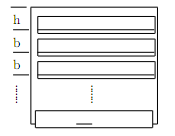
\includegraphics{./graphics/heightofpagebox.jpg}
\end{figure}
\end{comment}

\subsection{Dead cycles.} An execution of the OTR without shipping any material is called a \emph{dead cycle}. Dead cycles, have their uses and we will explain this a bit later on. However, long iterations that just return \textit{dead cycles} is an indication of an error somewhere. \tex counts the number of dead cycles in a counter named |\deadcycles| and stops the run if |\deadcycles >= \maxdeadcycles|.  In the \textit{plain} format |\maxdeadcycles| is set as 25 and in \latex as \the\deadcycles. |\maxdeadcycles = 100| is \the\maxdeadcycles. Each time |\shipout| is invoked, it resets |\deadcycles| to zero.

\begin{dispListing}
If the file is not included, reset \deadcycles, so that a long list of non-included
files does not generate an `Output loop' error.
115 \deadcycles\z@
116 \@nameuse{cp@#1}%
117 \fi
118 \let\@auxout\@mainaux}
\end{dispListing}


\subsection{\tex's Page Number.} The page number can come from any source. Salomon provides an example where the \textsc{OTR} typesets a page number from a |\count| variable. This is typeset centered below the printed area.

%\newpage
%
%Test
%\makeatletter
%
%\let\ltxxoutput\output
%\let\ltxlabel\label@name
%\output={{\let\label@name\@gobble
%  \shipout\vbox{
%  \box255\smallskip
%  \centerline{\thepage}}}
%}
%
%\vfill \penalty-10000
%
%\global\let\output\ltxxoutput
%\let\label@name\ltxlabel
%
%
%\makeatother


Notice that the output macro, just passes the contents of the box to |\shipout|. This is not actually a very good method, but is shown here to illustrate a point.

Note the |\tenrm| in the preceding example. It
is necessary because of the asynchronous nature of
the \otr. When the \otr is invoked, \tex can be
anywhere on the next page. Specifically, it could
be inside a group where a different font is used.
Without the |\tenrm|, that font (the current font)
would be used in the otr.
In the plain format, the |\count0| variable
serves as the page number, and the following two
macros are especially useful.




\subsection{The \texttt{\textbackslash vsplit} operation.} 

Supposed you have inserted the material required to go on a page on a big |\vbox|, but the material is a bit extra that what is required to fill a page exactly. You would need an operation to split the box in two. The |vsplit| operation does that. It is important to the understanding of OTR operations to have an intimate knowledge of |\vsplit|. Its syntax is: 

\begin{quote}
|\vsplit|\meta{box number} to \meta{dim}
\end{quote}

The result of the operation is a box. Most often it appears in an assignment such as: 

\begin{quote}
|\setbox1=\vsplit0 to2.6in| 
\end{quote}

This sets |\box1| to a
height of 2.6in, moves material from the top of
|\box0| to |\box1|, and keeps the remainder in |\box0|.

\begin{macro}{\loremlines}
It is important to remember that most of \tex's commands work with \latex as well. In Example~\ref{ex:loremlines}, we define a box to hold |lipsum| text in a two column layout. We want to define a macro that can split the box in as many lines as we require. 
\end{macro}

\begin{texexample}{Splitting a vbox}{ex:loremlines}
\newbox\one
\newbox\two
\long\gdef\loremlines#1#2{%
   \setbox\one=\vbox {#2}
   \setbox\two=\vsplit\one to #1\baselineskip
   \unvbox\two
   \gdef\boxone{#2}
}
\begin{multicols}{2}
\small
\loremlines{16}{\onepar}
\end{multicols}
\boxone

\setbox\one=\vbox{100}
\the\ht\one \\
\the\baselineskip
\the\splittopskip

\end{texexample}


\tex assumes that the new |\box1| may have to
be shipped out as part of the page. It therefore
places a glue similar to $h$ at the top of |\box1|.
This glue is called \docAuxCommand{splittopskip} and has a plain
format value of 10pt [348].

One important thing to note is that a box can only be split \textit{between} lines of text. 
If we split a box to another size, |\box1| will come out underfull.

Here is an \otr which splits the page, ships
out the top part and returns the rest to the MVL
(actually, to the recent contributions):

\begin{teXXX}
\output={\setbox0=\vsplit255 to1in
\shipout\box0 \unvbox255}
\end{teXXX}






\section{Communicating with the OTR: Marks}


The user can pass information to the output routine through \textit{marks}. Marks have the syntax

\begin{teX}
\mark{mark text}
\end{teX}

which is put in a mark item on the current vertical list. The mark text is subject to expansion
as in \cs{edef}.
If the mark is given in horizontal mode it migrates to the surrounding vertical lists like an
insertion item (see page Text By Topic 77); however, if this is not the external vertical list, the output routine
will not find the mark.

Marks are the main mechanism through which the output routine can obtain information
about the contents of the currently broken-off page, in particular its top and bottom. TEX sets
three variables:

{\obeylines
\cs{botmark} the last mark occurring on the current page;
\cs{firstmark} the first mark occurring on the current page;
\cs{topmark} the last mark of the previous page, that is, the value of \cs{botmark} on the previous
page.
}



If no marks have occurred yet, all three are empty; if no marks occured on the current page, all three variables are equal to the \cs{botmark} of the previous page. 

Marks can be used to get a section heading into the headline or footline of the page.

\begin{quote}
\begin{verbatim}
\def\section#1{ ... \mark{#1} ... }
\def\rightheadline{\hbox to \hsize
    {\headlinefont \botmark\hfil\pagenumber}}
\def\leftheadline{\hbox to \hsize
   {\headlinefont \pagenumber\hfil\firstmark}}
\end{verbatim}
\end{quote}

This places the title of the first section that starts on a left page in the left
headline, and the title of the last section that starts on the right page in
the right headline. Placing the headlines on the page is the job of the output
routine; see below.

It is important that no page breaks can occur in between the mark and the
box that places the title:

\emphasis{mark,nobreak}
\begin{teXXX}
\def\section#1{ ...
   \penalty\beforesectionpenalty
   \mark{#1}
   \hbox{ ... #1 ...}
   \nobreak
   \vskip\aftersectionskip
   \noindent}
\end{teXXX}

%%%%%%%%%%%% macro to put TeX references in right margin %%%%%%%% 
\newdimen\theight 
\def \TeXref#1{% 
             \vadjust{\setbox0=\hbox{\sevenrm\quad\quad\TeX book: #1}% 
             \theight=\ht0 
             \advance\theight by \dp0    \advance\theight by \lineskip 
             \kern -\theight \vbox to \theight{\rightline{\rlap{\box0}}% 
             \vss}% 
             }}% 
%%%%%%%%%%%%%%%%%%%%%%%%%%%%%%%%%%%%%%%%%%%%%%%%%%%%%%%%%%%%%%%%%%%%%%%%% 
 
However, useful these marks, sometimes an output routine (such as those found in \latexe needs to know why it was invoked. Knuth discusses in the \TeXref{396}  another method
that involves the value of the |\outputpenalty|. 
By testing for this value, it is possible to see what penalty occurred at a breakpoint;
any penalty of −10000, −10001, −10002, or less, forces the output routine to
act, hence different penalty values can be used to pass different messages. (When
the output routine puts material back on the list of contributions, it need not restore
the penalty at the breakpoint.) If output has been forced by a highly negative value
of |\outputpenalty|, the output routine can use |\vbox{\unvcopy255}| to discover how
full the page-so-far actually is. Underfull and overfull boxes are not reported when
|\box255| is packaged for use by the output routine, so there’s no harm in ejecting a
page prematurely if you want to pass a signal. (Set |\holdinginserts| positive to pass
a signal when the contents of |\box255| will be sent back through the page builder again,
if any insertions are present.)

Knuth also suggested another method that he called the \emph{dirtiest trick of all} that uses the depth 
of |\box255|. 

\section{Insertions}
Insertions are considered one of  the most  complex  topics in \tex. Many users master  topics  such 
as tokens,  file  I/O, macros,  and  even  OTRS  before they dare  tackle  insertions.  The  reason  is  that 
insertions  are  complex,  and  The \texbook, while 
covering all the relevant material, is somewhat cryptic regarding  insertions, and  lacks  simple examples. 
The  main  discussion  of  insertions takes  place  on 
[115-1251.  where \tex' s  registers  are also discussed. 
Examples  of  insertions are  shown, mostly  without 
explanations,  on  [363-364,  423-424].  A lot of what is described here is based on an article in TUGboat by David Salomon\footnote{\protect\url{http://www.tug.org/TUGboat/Articles/tb11-4/tb30salomon.pdf}}

Many users understand the idea of floats. Certain material to be typeset needs to be held in a buffer and inserted at different points on a page, for example a a figure that does not fit on a page it has to be inserted at the top of the next page. An \textit{insertion} is just a piece of a document that is generated at a certain point but appears at another point. Common examples are figures, footnotes and endnotes. Quoting Knuth:

\begin{quote}
  This  algorithm  is  admittedly  complicated, 
but  no  simpler  mechanism  seems  to  do  nearly 
as  much.
\end{quote}

\section{\protect\textbackslash shipout}

The primitive control sequence \docAuxCommand{shipout} is \tex's end game. It's syntax is quite simple:

\begin{quote}
|\shipout<box>|
\end{quote}

From TeXbook, Chapter 23: Output Routines, page 254:

\begin{quotation}
TeX’s primitive command |\shipout<box>| is what actually causes output. It sends the contents of the box to the dvi file, which is TeX’s main output file; after TeX has finished, the dvi file will contain a compact device-independent encoding of instructions that specify exactly what should be printed. When a box is shipped out, TeX displays the values of |\count0| through |\count9| on your terminal, as explained in Chapter 15; these ten counters are also recorded in the dvi file, where they can be used to identify the page. All of the |\openout, \closeout|, and |\write| commands that appear inside of the box are performed in their natural order as that box is being shipped out. Since a |\write| command expands macros, as explained in Chapter 21, TeX’s scanning mechanism might detect syntax errors while a |\shipout| is in progress. If  |\tracingoutput| is nonzero at the time of a \cs{shipout}, the contents of the box being shipped are written into your log file in symbolic form. You can say \cs{shipout} anywhere, not only in an output routine.
\end{quotation}


We can say:

\emphasize{shipout,vbox}
\begin{teXXX}
\shipout\vbox{%
  \hrule
  \medskip
  \lipsum[1-5]
  \medskip
  
  This is a Test for shipout
  
  \hrule
}
\end{teXXX}

\shipout\vbox{%
  \hrule
  \medskip
  \lipsum[1-5]
  \medskip
  \centering
  \textbf{Sample: }{This is a Test for shipout}
  \hrule
}

Since the output box handled by \tex still holds material the page is shown in the previous page. There is no page numbers or headers and it just shows he lorem-ipsum text and a primitive caption at the bottom. I have written the example to show the difference between the logical and actual pages. TeX does not care how the page will look, it will assemble it put headers, page numbers and pass it on to shipout. Shipout will then insert it to the dvi file, which will hold all teh instructions to print a real page.

We can modify the example to add our head and foot. 

\begin{texcode}{Shipout}{ex:ship2}
This will print by the normal routine

\long\gdef\boxit#1#2{\hbox{\vrule \vbox{\hrule\kern#2pt\hbox{%
\kern#2pt\vbox{#1}\kern#2pt}\kern#2pt\hrule}\vrule}}

\makeatletter
\shipout\vbox {%
  \vskip\topsep\relax
  \vskip\headsep
   \@thehead
   \vskip30pt
    \boxit{
      \lipsum[1-5]
      }{2}
   \vskip30pt
   \@thefoot   
}
\makeatother 
\end{texcode}

\latexe's output routine takes care of all the page geometry, the details to set up the headers and footers, but most importantly intercepts teh contents of the output box measure it, cuts it inserts the inserts such as footnotes and figures, margin notes, separates the text in two columns if necessary and so on. 

\long\gdef\boxit#1#2{\hbox{\vrule \vbox{\hrule\kern#2pt\hbox{%
\kern#2pt\vbox{#1}\kern#2pt}\kern#2pt\hrule}\vrule}}
\makeatletter
\shipout\vbox {%
  \vskip\topsep\relax
  \vskip\headsep
   \@thehead
   \vskip30pt
    \boxit{
      \lipsum[1-5]
      }{2}
   \vskip30pt
   \@thefoot   
}
\makeatother 



An output routine will prepare the virtual page and pass it onto a 

Here is an OTR for a \textit{framed} page. It surrounds the
page with double rules on all sides, and centers the
page number below the double box. Note that the
page shipped out is wider and taller than \cs{box255}.
The value of \cs{hsize} in this case is, therefore, not
the width of the final page shipped out, but the
width of the text lines in \cs{box255}.

Macro \cs{frameit} typesets text and surrounds it
with 4 rules (see [Ex. 21.3]). Parameter \#2 is the
space between the rules and the text. \#1 is a box
containing the text.

\emphasis{output,shipout}
\begin{texcode}{Example of simple output routine}{ex:output1}
\def\frameit#1#2{%
 \vbox{\hrule
  \hbox{%
    \vrule \kern#2pt
      \vbox{\kern#2pt #1
         \kern#2pt}%
      \kern#2pt\vrule}
\hrule}}

\output={
   \shipout\vbox{
   \boxit{\frameit{\box255}9}
      \medskip
      \centerline{Test Framed Page}}
  \advancepageno}
\end{texcode}

 

So far we did not care if the height of the page is right or not. In production code the shipout holds
a box, which has been produced by \tex. Any material we add to it, must not affect the dimensions of the box.
If we do and is too big the drivers will probably clip it.


Plain TeX has an output routine that takes care of  simple things like page numbering and insertions
using \cs{footnote} and \cs{topinsert}. 


So far we have examined the \tex OTR in detail. I hope it has given you enough understanding, not only to write your own output routine, but also to now be ready to study the \latex output routine, which is much more complicated. We have so far seen that  when \tex 
is typesetting pages of continuous text, it will gather material until it can find a least-cost page break intended to
make the gathered material fit the \cs{pagegoal} size. The
gathered material will then be placed into |\box255| and
the output routine stored in the token register \cs{output}
will be processed in a group of its own. 

Usually it will
arrange the gathered material in some way, add headers,
footlines and page numbers, and ship the gathered results out in typeset form with the \cs{shipout} command.
At the time of the \cs{shipout} command all \cs{open} and
\cs{write} commands stored in the box shipped out are expanded and written out. This is what makes it possible to have page labels corresponding to the actual page
numbers at the time of shipout: the corresponding info
is written to the |.aux| file at that time.
The output routine may decide to place material
back on the main vertical list instead of shipping it out. Its ob is to check if it can have a break, if it can it will ship the page out. If it cannot it will palce the material back on the main vertical list. 

\section{\LaTeX\  output routines}


\LaTeX\ output routine is described in \texttt{ltoutput.dtx}. You should also have a look at \texttt{ltfloat.dtx}. The algorithm is revisited i \latex3 and Frank Mittelbach, published a paper
\footnote{\protect\url{http://www.latex-project.org/papers/xo-pfloat.pdf}} in which he explains some of the problems facing the team, when dealing with the output routine.


Information on the output routine is rather scarce. Best source is a series of  articles in the TUGBoat by David Salomon.

\href{http://www.tug.org/TUGboat/Articles/tb11-1/tb27salomon.pdf}{Output Routines: Examples and Techniques. Part I: Introduction and Examples.}

\href{http://www.tug.org/TUGboat/Articles/tb11-2/tb28salomon.pdf}{Output Routines: Examples and Techniques. Part II: OTR Techniques}

\href{http://www.tug.org/TUGboat/Articles/tb11-4/tb30salomon.pdf}{Output Routines: Examples and Techniques. 
Part III: Insertions}

\href{http://www.tug.org/TUGboat/Articles/tb15-1/tb42salomon-output.pdf}{Output routines: Examples and techniques Part IV: Horizontal techniques}


David Kastrup's article \href{http://www.tug.org/TUGboat/Articles/tb24-3/kastrup.pdf}{Output Routine Requirements for Advanced Typesetting Tasks} (Proceedings of EuroTEX 2003) otlined some of the difficult areas and specifications for generic routines

The standard blocks are well described above and most tasks could be accomplished 
by rather working from
standard building blocks like \textit{insertion lists}, \textit{here points},
default mechanisms for \textit{margin notes} and so on.


%\section{Calling the output routine}
%
%The output routine is called either by TeX's normal page-breaking
%mechanism, or by a macro putting a penalty < or = -10000 in the output
%list. In the latter case, the penalty indicates why the output
%routine was called, using the following code.
%penalty reason
%
%\begin{longtable}{ll}
%\toprule
%penalty &reason\\
%\midrule
%-10000  &\ pagebreak\\
%~       &\ newpage\\
%-10001  &clearpage (\ penalty -10000 \ vbox{}| \ penalty -10001)|\\
%-10002  &float insertion, called from horizontal mode\\
%-10003 &float insertion, called from vertical mode.\\
%-10004 &float insertion.\\
%\bottomrule
%\end{longtable}
%\medskip
%
%Note: A |float| or |marginpar| puts the following sequence in the output
%list: 
%
%\begin{enumerate}
%\item a penalty of -10004,
%
%\item a null |\vbox|
%
%\item a penalty of -10002 or -10003.
%\end{enumerate}
%
%This solves two special problems:
%
%\begin{enumerate}
%\item If the float comes right after a |\newpage| or |\clearpage|,
%then the first penalty is ignored, but the second one
%invokes the output routine.
%
%\item If there is a split footnote on the page, the second 'page'
%puts out the rest of the footnote
%\end{enumerate}
%
%\latex first defines some helper routines and increase the \cs{maxdeadcycles}. The helper macros are for
%manipulating lisst.
%
%\begin{teX}
% \maxdeadcycles = 100
% \let\@elt\relax
% \def\@next#1#2#3#4{\ifx#2\@empty #4\else
%   \expandafter\@xnext #2\@@#1#2#3\fi}
%   \@next \CS \LIST {NONEMPTY}{EMPTY} == %% NOTE: ASSUME
%\@elt = \relax
% BEGIN assume that \LIST == \@elt \B1 ... \@elt \Bn
% if n = 0
% then EMPTY
% else 
%   \CS :=L \B1
%   \LIST :=G \@elt \B2 ... \@elt \Bn
%   NONEMPTY
% fi
%END
%\end{teX}
%
%
%\begin{teX}
%11 \def\@xnext \@elt #1#2\@@#3#4{\def#3{#1}\gdef#4{#2}}
%
%12 \def\@testfalse{\global\let\if@test\iffalse}
%13 \def\@testtrue {\global\let\if@test\iftrue}
%14 \@testfalse}
%   }
%
%15 \def\@bitor#1#2{\@testfalse {\let\@elt\@xbitor
%16   \@tempcnta #1\relax #2}}
%
%17 \def\@xbitor #1{\@tempcntb \count#1
%18    \ifnum \@tempcnta =\z@
%19    \else
%20      \divide\@tempcntb\@tempcnta
%21    \ifodd\@tempcntb \@testtrue\fi
%22   \fi}
%\end{teX}
%
%
%\subsection{Float boxes and lists.} 
%A \textit{float list} consisting of the 
%floats in boxes |\boxa ... \boxN| has
%the form:
%
%|\@elt \boxa ... \@elt \boxN|
%where |\boxI| is defined by
%
%|\newinsert\boxI|
%
%Normally, |\@elt| is |\let| to |\relax|. A test can be performed on the
%entire 
%oat list by locally |\def|'ing |\@elt| appropriately and
%executing the list.
%This is a lot more efficient than looping through the list.
%\LaTeX\ defines float boxes as |bx@A| to |bx@R| to make them available for 
%inserts. These will be used later to define the lists that hold these boxes. 
%
%\latex now defines the float boxes. Each one is defined as an \cmd{\newinsert.}
%
%\begin{teXXX}
%\newinsert\bx@A
%...
%\newinsert\bx@I
%\newinsert\bx@J
%\newinsert\bx@K
%\newinsert\bx@L
%\newinsert\bx@M
%\newinsert\bx@N
%\newinsert\bx@O
%\newinsert\bx@P
%\newinsert\bx@Q
%\newinsert\bx@R
%\end{teXXX}
%
%
%
%Once these boxes are defined they are inserted in the |@freelist|. At this point all the other lists are defined.
%
%\emphasis{@freelist,@toplist,@botlist,@midlist,@currlist}
%\begin{teXXX}
%41 \gdef\@freelist{\@elt\bx@A\@elt\bx@B\@elt\bx@C\@elt\bx@D
%         \@elt\bx@E
%42                 \@elt\bx@F\@elt\bx@G\@elt\bx@H\@elt\bx@I\@elt\bx@J
%43                 \@elt\bx@K\@elt\bx@L\@elt\bx@M\@elt\bx@N
%44                 \@elt\bx@O\@elt\bx@P\@elt\bx@Q\@elt\bx@R}
%\end{teXXX}
%
%\startlineat{45}
%All the lists are defined initially to be empty.
%\begin{teXXX}
%45 \gdef\@toplist{}
%46 \gdef\@botlist{}
%47 \gdef\@midlist{}
%48 \gdef\@currlist{}
%49 \gdef\@deferlist{}
%50 \gdef\@dbltoplist{}
%51 \gdef\@dbldeferlist{}
%\end{teXXX}
%
%
%The lists are similar to those defined in \texttt{plain}.
%
%\begin{description}
%\item[\cs{@freelist}] : List of empty boxes for placing new 
%floats.
%\item[\string\@toplist] : List of 
%floats to go at top of current column.
%\item[\string\@midlist] : List of 
%floats in middle of current column.
%\item[\string\@botlist] : List of 
%floats to go at bottom of current column.
%\item[\string\@deferlist] : List of 
%floats to go after current column.
%\item[\string\@dbltoplist] : List of double-col. 
%floats to go at top of current
%page.
%\item[\string\@dbldeferlist] : List of double-column 
%floats to go on subsequent
%pages.
%
%\end{description}
%
%\begin{multicols}{2}
%Check was prudent when defining the newinsert boxes in order to reserve space and memory. The package \docpkg{morefloats} can be used to add more floats to this list. This should have definitely been included here in a revision.
%
%\subsection{Defining Layout parameters} All the page layout parameters are defined next. 
%
%\begin{teXXX}
%52 \newdimen\topmargin
%53 \newdimen\oddsidemargin
%54 \newdimen\evensidemargin
%55 \let\@themargin=\oddsidemargin
%56 \newdimen\headheight
%57 \newdimen\headsep
%58 \newdimen\footskip
%59 \newdimen\textheight
%60 \newdimen\textwidth
%61 \newdimen\columnwidth
%62 \newdimen\columnsep
%63 \newdimen\columnseprule
%64 \newdimen\marginparwidth
%65 \newdimen\marginparsep
%66 \newdimen\marginparpush
%\end{teXXX}
%
%Remember  that TeX knows little about a page. The problem is that TEX has no idea how
%wide and tall the paper is. All it knows is the
%left and top offsets, and the dimensions of the
%printed area (|\hsize| and |\vsize|). All these dimensions need to be calculated and adjustments made within the \otr.
%
%A document normally  starts by specifying:
%
%\begin{teXXX}
%\newdimen\paperheight
%\newdimen\paperwidth
%\paperheight=..in \paperwidth=..in
%\end{teXXX}
%
%
%\end{multicols}
%
%
%\subsection*{The AtBeginDvi}
%A box register is used  to put stuff that must appear before anything else
%in the |.dvi| file.
%
%The stuff in the box should not add any typeset material to the page when it
%is unboxed.
%
%\emphasis{AtBeginDvi,@begindvibox}
%
%\begin{teXXX}
%67 \newbox\@begindvibox
%68 \def \AtBeginDvi #1{%
%69 \global \setbox \@begindvibox
%70 \vbox{\unvbox \@begindvibox #1}%
%71 }
%\end{teXXX}
%
%\begin{teXXX}
%72 \newdimen\@maxdepth
%73 \@maxdepth = \maxdepth
%\end{teXXX}
%
%
%Some new registers for paperheight and paperwidth are defined:
%
%\begin{teXXX}
%74 \newdimen\paperheight
%75 \newdimen\paperwidth
%76 \newif \if@insert
%These should definitely be global:
%77 \newif \if@fcolmade
%78 \newif \if@specialpage \@specialpagefalse
%These should be global but are not always set globally in other les.
%79 \newif \if@firstcolumn \@firstcolumntrue
%80 \newif \if@twocolumn \@twocolumnfalse
%Not sure about these: two questions. Should things which must apply to a whole
%doument be local or global (they probably should be `preamble only' commands)?
%Are these three such things?
%81 \newif \if@twoside \@twosidefalse
%82 \newif \if@reversemargin \@reversemarginfalse
%83 \newif \if@mparswitch \@mparswitchfalse
%This counter has been imported from `multicol'.
%84 \newcount \col@number
%85 \col@number \@ne
%\end{teXXX}
%
%and a lot of other internal registers
%
%\begin{teX}
%86 \newcount\@topnum
%87 \newdimen\@toproom
%88 \newcount\@dbltopnum
%89 \newdimen\@dbltoproom
%90 \newcount\@botnum
%91 \newdimen\@botroom
%92 \newcount\@colnum
%93 \newdimen\@textmin
%94 \newdimen\@fpmin
%95 \newdimen\@colht
%96 \newdimen\@colroom
%97 \newdimen\@pageht
%98 \newdimen\@pagedp
%99 \newdimen\@mparbottom \@mparbottom\z@
%100 \newcount\@currtype
%101 \newbox\@outputbox
%102 \newbox\@leftcolumn
%103 \newbox\@holdpg
%104 \def\@thehead{\@oddhead} % initialization
%105 \def\@thefoot{\@oddfoot}
%\end{teX}
%
%
%\subsection{\texttt{\textbackslash clearpage}}
%
%\begin{macro}{\clearpage}
%The clearpage macro is a bit complicated, as it needs to avoid a complete empty page after a |\twocolumn[..]|. This prevents the text from the argument
%vanishing into a  float box, never to be seen again. We hope that it does not
%produce wrong formatting in other cases.
%\end{macro}
%
%\begin{teXXX}
%106 \def\clearpage{%
%107   \ifvmode
%108   \ifnum \@dbltopnum =\m@ne
%109     \ifdim \pagetotal <\topskip
%110       \hbox{}%
%111     \fi
%112   \fi
%113  \fi
%114 \newpage
%115 \write\m@ne{}%
%116 \vbox{}%
%117 \penalty -\@Mi
%118 }
%\end{teXXX}
%
%\subsection{The \texttt{\textbackslash clearpagedoublepage} macro} 
%
%\begin{macro}{cleardoublepage}
%This checks for odd and even pages by using the
%page counter |c@page|.  It also provides switches of twoside printing. 
%
%\numberlineat{119}
%\begin{teXXX}
%\def\cleardoublepage{%
%   \clearpage
%   \if@twoside 
%     \ifodd\c@page
%     \else
%       \hbox{}
%       \newpage
%       \if@twocolumn\hbox{}\newpage
%       \fi
%     \fi
%  \fi}
%\end{teXXX}
%\end{macro}
%
%Note the |\newpage| is defined a bit further on. This is a fairly simple definition, since most of the code that follows only gets a bit complicated with the twocolumn option. It sets the dimensions and the booleans to those appropriate for the |onecolumn| option. An important note we back to \tex's |\hsize|. Both the linewidth as well as the columnwidth are set to this.
%
%\begin{teXXX}
%123 \def\onecolumn{%
%124   \clearpage
%125   \global\columnwidth\textwidth
%126   \global\hsize\columnwidth
%127   \global\linewidth\columnwidth
%128   \global\@twocolumnfalse
%129   \col@number \@ne
%130   \@floatplacement
%     }
%\end{teXXX}
%
%\subsection{\string newpage.} 
%
%The |\newpage| macro is programmed defensively. The two checks at the beginning ensure that an item label or run-in section title
%immediately before a |\newpage| get printed on the correct page, the one before
%the page break.
%All three tests are largely to make error processing more robust; that is why
%they all reset the 
%flags explicitly, even when it would appear that this would be
%done by a |\leavevmode|.
%
%\begin{teXXX}
%131 \def \newpage {%
%132  \if@noskipsec
%133    \ifx \@nodocument\relax
%134      \leavevmode
%135      \global \@noskipsecfalse
%136    \fi
%137 \fi
%138 \if@inlabel
%139   \leavevmode
%140   \global \@inlabelfalse
%141 \fi
%142 \if@nobreak \@nobreakfalse \everypar{}\fi
%143 \par
%144 \vfil
%145 \penalty -\@M}
%\end{teXXX}
%
%An empty cols is defined. There is a note here, that an invisible rule might have been a better idea.
%
%\begin{teXXX}
%146 \def \@emptycol {\vbox{}\penalty -\@M}
%\end{teXXX}
%
%\subsection{The \string twocolumn macro.} This is the longest definition so far. We will leave it for a while and then come back. There are several bug fixes to the two-column stuff here. Firstly, like the onecolumn the page parameters are set to the correct parameters.
%
%
%\begin{teXXX}
%147 \def \twocolumn {%
%148 \clearpage
%149 \global\columnwidth\textwidth
%150 \global\advance\columnwidth-\columnsep
%151 \global\divide\columnwidth\tw@
%152 \global\hsize\columnwidth
%153 \global\linewidth\columnwidth
%154 \global\@twocolumntrue
%155 \global\@firstcolumntrue
%156 \col@number \tw@
%\end{teXXX}
%
%
%
%\section{The output macro}
%
%The setting of the \cs{output} is quite short but it belies its complexity.
%After having checked verious parameters it redirects to |@specialoutput|. This is the heart of the routines. Notice that \latex just fills in the token list of \tex's |output| routine, it does not attempt to redefine it or save it. 
%Should some hooks be defined here, life might have been made easier, however, what one can do is to first save the \latex output routine and then redefine the output as one may wish. Return to it can happen after it. If you take this approach, you should be careful of packages that redefine output, such as |multicol| and |longtable|. An approach such as this is taken by \citeauthor{revtex} in the \pkgname{revtex} class.\footcite[][This is a document class of the American Physical Society. It enables submission to any of the APS journals. Its distribution point is \protect\url{http://publish.aps.org/revtex4/}]{revtex}
%
%\emphasis{ifnum,fi,else,ifdimen,@specialoutput}
%\begin{teX}
%204 \output {%
%205 \let \par \@@par
%206 \ifnum \outputpenalty<-\@M
%207    \@specialoutput
%208 \else
%209    \@makecol
%210    \@opcol
%211    \@startcolumn
%212    \@whilesw \if@fcolmade \fi
%213      {%
%218      \@opcol\@startcolumn}%
%219 \fi
%220 \ifnum \outputpenalty>-\@Miv
%221 \ifdim \@colroom<1.5\baselineskip
%222 \ifdim \@colroom<\textheight
%223 \@latex@warning@no@line {Text page \thepage\space
%224 contains only floats}%
%225 \@emptycol
%226 % \if@twocolumn
%227 % \if@firstcolumn
%228 % \else
%229 % \@emptycol
%230 % \fi
%231 % \fi
%232 \else
%  233 \global \vsize \@colroom
%234 \fi
%235 \else
%236   \global \vsize \@colroom
%237 \fi
%238 \else
%239   \global \vsize \maxdimen
%240 \fi
%241 }
%\end{teX}
%
%
%
%\begin{teXXX}
%244 \gdef\@specialoutput{%
%245   \ifnum \outputpenalty>-\@Mii
%246     \@doclearpage
%247   \else
%248     \ifnum \outputpenalty<-\@Miii
%249         \ifnum \outputpenalty<-\@MM \deadcycles \z@ \fi
%250                 \global \setbox\@holdpg \vbox {\unvbox\@cclv}%
%251         \else
%252         \global \setbox\@holdpg \vbox{%
%253                 \unvbox\@holdpg
%254                 \unvbox\@cclv
%We must now remove the box added by the 
%oat mechanism and the \topskip
%glue therefore added above it by TEX.
%255                \setbox\@tempboxa \lastbox
%256                \unskip
%257 }%
%These two are needed as separate dimensions only by \@addmarginpar; for other
%purposes we put the whole size into \@pageht (see below).
%258                \@pagedp \dp\@holdpg
%259                \@pageht \ht\@holdpg
%260                \unvbox \@holdpg
%
%261                \@next\@currbox\@currlist{%
%262                \ifnum \count\@currbox>\z@
%Putting the whole size into \@pageht (see above).
%263                  \advance \@pageht \@pagedp
%264                  \ifvoid\footins \else
%265                    \advance \@pageht \ht\footins
%266                    \advance \@pageht \skip\footins
%267                    \advance \@pageht \dp\footins
%268                \fi
%\end{teXXX}
%
%
%
%\subsection{The \string @doclearpage macro.} This is an emergency action. It dumps everything: footnotes first and then floats. 
%
%
%\section*{The Kludgeins}
%
%The kludgeins are simply inserts that fool \tex in enlarging a page by a small amount, normally used to allow one or two lines of text to go in the same page.
%
%The two kludgeins mentioned in the kernel are are \cs{enlargethisspace} and its star version.\footnote{The Oxford English Dictionary (2nd ed., 1989) kludge entry cites one source for this word's earliest recorded usage, definition, and etymology: Jackson W. Granholm's 1962 "How to Design a Kludge" article, which appeared in the American computer magazine Datamation
%kludge  Also kluge. [J. W. Granholm's jocular invention: see first quot.; cf. also bodge v., fudge v.]
%
%'An ill-assorted collection of poorly-matching parts, forming a distressing whole' (Granholm); esp. in Computing, a machine, system, or program that has been improvised or 'bodged' together; a hastily improvised and poorly thought-out solution to a fault or 'bug'.
%
%The word 'kludge' is...derived from the same root as the German Kluge..., originally meaning 'smart' or 'witty'.... 'Kludge' eventually came to mean 'not so smart' or 'pretty ridiculous'.}
%
%
%
%\begin{teXX}
%\gdef \enlargethispage{%
%1198 \@ifstar
%1199 {%
%1203   \@enlargepage{\hbox{\kern\p@}}}%
%1204 {%
%1208   \@enlargepage\@empty}%
%1209 }
%\end{teXX}
%
%Adds |<dim>| to the height of the current column only. On the printed page the
%bottom of this column is extended downwards by exactly |<dim>| without having
%any effect on the placement of the footer; this may result in an overprinting.
%\cs{enlargethispage}.
%
%Similar to |\enlargethispage| but it tries to squeeze the column to be printed
%in as small a space as possible, ie it uses any shrinkability in the column. If the
%column was not explicitly broken (e.g. with |\pagebreak|) this may result in an
%overfull box message but except for this it will come out as expected (if you know
%what to expect).
%The star form of this command is dedicated to Leslie Lamport, the other we
%need for ourselves (FMi, CAR).
%These commands may well have unwanted if used soon before a\ldots
%
% 




\section{Packages}

OTR routines are notoriously difficult to debug and define. Some of the available packages at CTAN
can make the programming job easier.

The \pkg{everypage} package by Sergio Callegari provides hooks into the \latex\ internal commands to
to do actions on every page or on the current page. Specifically, actions  are performed \emph{before} the page is shipped, so they can be used to put watermarks \emph{in the background} of a page, or to
set the page layout. 

The package provides two hooks:

\emphasis{AddEverypageHook,AddThisPageHook}
\begin{teXXX}
  \AddEverypageHook{Test}
  \AddThisPageHook
\end{teXXX}

The package reminds in some sense
\pkgname{bobhook} by Karsten Tinnefeld, but it differs in the way in
 which the hooks are implemented, as detailed in the following.
 In some sense it may also be related to the package
 \pkgname{everyshi} by Martin Schroeder, but again the implementation
 is different.

 
 This program adds two \LaTeX\ hooks that get run when document
 pages are finalized and output to the |.dvi| or |.pdf|
 file. Specifically, one hook gets executed on every page, while the
 other is executed for the current page. Hook actions are are performed
 \emph{before} the page is output on the medium, and this is
 important to be able to play with the page layout or to put things
 \emph{behind} the page contents (e.g., watermarks such as an image,
 framing, the ``DRAFT'' word, and the like).
 
 The package reminds in some sense \pkg{bobhook} by Karsten
 Tinnefeld, but it differs in the way in which the hooks are
 implemented:
 


 \begin{enumerate}
 \item there is no formatting inherent in the hooks. If one wants to
   put some watermark on a page, it is his own duty to put in the
   hook the code to place the watermark in the right position. Also
   note that the hooks code should \emph{eat up no space} in the
   page.  Again, if the hooks are meant to place some material on the
   page, it is the duty of the hook programmer to put code in the
   hooks to pretend that the material has zero width and zero height.
   The implementation is \emph{lighter} than the \Lpack{bobhook} one,
   and possibly more flexible, since one is not limited by any
   pre-coded formatting for the hooks. On the other hand it is
   possibly more difficult to use. Nonetheless, it is easy to think
   of other packages relying on \Lpack{everypage} to deliver more
   user-friendly and \emph{task specific} interfaces. Already there
   are a couple of them: the package \Lpack{flippdf} produces
   mirrored pages in a PDF document and \Lpack{draftwatermark}
   watermarks document pages.
 \item similarly to \Lpack{bobhook} and \Lpack{watermark}, the
   package relies on the manipolatoin of the internal \LaTeX\ macro
   |\@begindvi| to do the job. However, the redefinition of
   |\@begindvi| is here postponed as much as possible, striving to
   avoid interference with other packages using |\AtBeginDvi| or
   anyway manipulating |\@begindvi|. Specifically \Lpack{everypage}
   makes no special assumption on the initial code that |\@begindvi|
   might contain.
 \end{enumerate}



Also in some sense \pkgname{everypage} can be related to package
 \pkgname{everyshi} by Martin Schr\"oeder \cite{everyshi}, but it differs radically from
 it in the implementation. In fact,\pkgname{everypage} operates by
 manipulation of the |\@begindvi| macro, rather than at the
 lower level |\shipout| macro.

\section{hooking at shipout}

\begin{docCmd} {EveryShipout} {}
\begin{docCmd} {AtNextShipout} {}
This package provides the hooks \cs{EveryShipout} and 
  \cs{AtNextShipout} whose arguments are executed after the output 
  routine has constructed \cs{box255}, and before \cs{shipout} is 
  called.
\end{docCmd}
\end{docCmd}

An example application for this package would be a package for
 adding text to the bottom of each page.
 The  \pkgname{prelim2e} package adopts this method \citep{prelim2e}.\footcite{prelim2e}

The solution  uses is based on code developed in  |quire.tex| by
 Marcel R.~van der Goot.\footcite{quire}  

The \pkgname{prelim2e}  intercepts and modifies the |\box255|. 

\begin{teX}
44 \newcommand{\@Prelim@EveryShipout}{%
45 \bgroup
% First we save the dimensions of \box255: height, width and depth; and calculate
% the total height of \box255.
46 \dimen\z@=\wd\@cclv
47 \dimen\@ne=\ht\@cclv
48 \dimen\tw@=\dp\@cclv
49 \dimen\thr@@=\dimen1
50 \advance\dimen\thr@@ by \dimen\tw@
% Then we set \box255: A \vbox to the total height of \box255. In this a \hbox to
% the width of \box255 is included, in which \box255 is set.
51 \global\setbox\@cclv\vbox to \dimen\thr@@{%
52 \hb@xt@\dimen\z@{%
53 \box\@cclv%
54 \hss
55 }%
\end{teX}
To this we append the text produced by |\PrelimText|. It is put in a |\vbox to 0pt|
in which a |\hbox| to the width of |\box255| is included, in which |\PrelimText| is set.
We have to reset |\protect| because it is set to |\noexpand| by the output routine.

\begin{teXXX}
56 \vbox to \z@{%
57   \hb@xt@\dimen\z@{%
58     \let\protect\relax
59     \hfill\PrelimText\hfill
60   }%
61   \vss
62 }%
63   \vss
64 }%
\end{teXXX}

Finally we set the dimensions of |\box255| to the values they had before |\@Prelim@EveryShipout|.

\begin{teX}
65 \wd\@cclv=\dimen\z@
66 \ht\@cclv=\dimen\@ne
67 \dp\@cclv=\dimen\tw@
68 \egroup
69}
\end{teX}

Once the command is defined, it is hooked into the system via |\EveryShipout| when it is in draft mode. 

\begin{teX}
70 \if@prelim@draft
71 \EveryShipout{\@Prelim@EveryShipout}
72 \fi
\end{teX}

\section{How to place a background image}

One can use \tikzname to place a background image or some text on a page

First we define some utility macros:


\begin{teX}
\def\bg@contents{Draft}
\def\bg@color{red!45}
\def\bg@angle{60}
\def\bg@opacity{.5}
\def\bg@scale{15}
\def\bg@position{current page.center}
\def\bg@anchor{}
\def\bg@hshift{0}
\def\bg@vshift{0}
\end{teX}

A new command is then developed to describe the background material

\begin{teXXX}
\newcommand\bg@material{%
   \begin{tikzpicture}[remember picture,overlay]
   \node [rotate=\bg@angle,scale=\bg@scale,opacity=\bg@opacity,%
   xshift=\bg@hshift,yshift=\bg@vshift,color=\bg@color]
   at (\bg@position) [\bg@anchor] {\bg@contents};
  \end{tikzpicture}}%
\end{teXXX}


Once the background material has been defined we can place it on the page by simply calling:

\begin{teX}
\newcommand\BgThispage{\AddThispageHook{\bg@material}}
\end{teX}


The \pkgname{background}\footcite{background} package by \citeauthor has capitalized on two good packages the \tikzname and the \pkgname{everypage}.
\footcite{everypage} As most of modern
\tex programming works with |pdf| files, package developers prefer to use \tikzname methods for hooking directly into the pdf and thus avoid a trip into the output routine. If it is required then it hooks via the dvi or shipout commands.\footnote{These packages are loaded automatically by the \pkgname{phd-pkgmanager}.}



\vfill

\message{(total: \the\pagetotal
depth: \the\pagedepth
shrink: \the\pageshrink
stretch: \the\pagestretch}



 







































% 
%</driver>
% \fi
% 
%  \CheckSum{0}
%  \CharacterTable
%  {Upper-case    \A\B\C\D\E\F\G\H\I\J\K\L\M\N\O\P\Q\R\S\T\U\V\W\X\Y\Z
%   Lower-case    \a\b\c\d\e\f\g\h\i\j\k\l\m\n\o\p\q\r\s\t\u\v\w\x\y\z
%   Digits        \0\1\2\3\4\5\6\7\8\9
%   Exclamation   \!     Double quote  \"     Hash (number) \#
%   Dollar        \$     Percent       \%     Ampersand     \&
%   Acute accent  \'     Left paren    \(     Right paren   \)
%   Asterisk      \*     Plus          \+     Comma         \,
%   Minus         \-     Point         \.     Solidus       \/
%   Colon         \:     Semicolon     \;     Less than     \<
%   Equals        \=     Greater than  \>     Question mark \?
%   Commercial at \@     Left bracket  \[     Backslash     \\
%   Right bracket \]     Circumflex    \^     Underscore    \_
%   Grave accent  \`     Left brace    \{     Vertical bar  \|
%   Right brace   \}     Tilde         \~}
%
%
%
% \changes{1.0}{2013/01/26}{Converted to DTX file}
%
% \DoNotIndex{\newcommand,\newenvironment}
% \GetFileInfo{phd.dtx}
% 
%  \def\fileversion{v1.0}          
%  \def\filedate{2012/03/06}
% \title{The \textsf{phd} package.
% \thanks{This
%        file (\texttt{phd.dtx}) has version number \fileversion, last revised
%        \filedate.}
% }
% \author{Dr. Yiannis Lazarides \\ \url{yannislaz@gmail.com}}
% \date{\filedate}
%
%
% 
% ^^A\maketitle
% 
% ^^A\frontmatter
%  ^^A\coverpage{./images/hine02.jpg}{Book Design }{Camel Press}
%  \newpage
% ^^A\secondpage
% \pagestyle{empty}
%
%
% 
%
%
% \pagestyle{headings}
% \raggedbottom
% ^^A \StopEventually{}
%  \OnlyDescription
%
%  ^^A\StopEventually{\printindex}
%<*package>
% \CodelineNumbered
% \pagestyle{headings}
% 
%
% \part{IMPLEMENTATION}
% 

% \chapter{Implementation Strategy}
%
% The implementation is divided into different parts. 
% These parts are sometimes placed smaller packages 
% to make their maintenance easier and also to enable,
% partial deployment.
% 	
% \begin{description}
%
%  \item[The Package Manager] This section is responsible 
%       for pre-loading  packages, resolving conflicts and 
%       providing all interfacing commands (see \docFile{phd-pkgmanager}).
%
%  \item[The Headings Layouts Manager] This section manages 
%       the design of complex layouts for sectioning commands.
%
%  \item[The Table of Contents Manager] Manages the typesetting of
%       contents pages.
%
%  \item [Color Management] Color is managed in a consistent manner
%        through a concept of color palettes.
%
%  \item [The header and footer Manager] Manages the typesetting of 
%        headers and footers.
%
%  \item [lists] Formats lists.
%
%  \item [quote] Provides environments and keys for quotes and quotations.
%
%  \item [Indexing and Documentation] This is managed through the
%        package \pkgname{phd-documentation}.
%
%  \item [The Image Page Manager] This section manages the design of 
%       pages that consist primarily of images and complex
%		page layouts.
%
%  \item[Common Utilities] We provide a number of predefined commands
%		for macros that us and other people found useful.
%
%  \item [Handlers] The phd-handlers package provides handlers for managing
%    key definitions, in a consistent way.
%
%  \item[Scripts Manager] Manages the loading of scripts for the worlds 
%  laguages and scripts.
%
%  \item[Keys] Key values are managed through \pgfname. The package
%       \pkg{phd-handlers} provides some useful handlers, mostly used by
%       internally.
%
%  \item[Epigraphs] A small supplementary package for epigraphs.
%
%  \item[MWE] The package generates a large number
%		of Minimum Working Examples that we use for testing. 
%		Most of them can also used as examples for training 
%		or self-study.
%
%  \item[Counters] The package counters, is an extension to the current
%    \latexe package offering more functionality and close integration
%    with the rest of the |phd| packages.
%
% \end{description}
%
% \section{Preliminaries}
%
% The basic requirement for the Package Manager is to load
% an adequate number of packages to enable the typesetting
% of a diverse number of large documents without requiring
% additional packages to be loaded by typical groups of
% authors. This has its advantages, but of course it does 
% slow things down. A long term objective is to select
% packages depending as an option on the type of document
% being prepared.
%
% \subsection{Preliminaries}
%
%    Standard file identification. We first announce the package 
%	 and require that it be used with \LaTeX2e. RE
%
%    \begin{macrocode}
\NeedsTeXFormat{LaTeX2e}[2017/04/15]%
\ProvidesPackage{phd}[2015/1/13 v1.0 less preamble (YL)]%
\let\ltxtoday\today
\newcommand\U[1]{{\texttt{U+#1}}(\char"#1)\xspace}
\let\latexitemize\itemize
\let\latexenditemize\enditemize
\let\latexenumerate\enumerate
\let\latexendenumerate\endenumerate
%    \end{macrocode}

% Load the package \pkgname{fixltx2e} to update \LaTeX2e for various fixes. The package fixes a number things in the LaTeX2e kernel. Due to LaTeX's stability policy, these corrections have not been incorporated into the LaTeX2e kernel, but this package does things most people would agree are bugfixes. So to load this package is always recommended for newly created documents. The corrections have no commonalities, but the package's description has a nice summary:
%
%ensure one-column floats don't get ahead of two-column floats;
%correct page headers in twocolumn documents;
%stop spaces disappearing in moving arguments;
%allowing |\fnsymbol| to use text symbols;
%allow the first word after a float to hyphenate;
% cs{emph} can produce caps/small caps text;
%bugs in \cs{setlength} and \cs{flushbottom.}
% 
%    \begin{macrocode}
%\RequirePackage{fixltx2e}[2006/03/24]
% mock chapters where necessary
\@ifundefined{c@chapter}{%  
      \newcounter{chapter}
      \def\thechapter{\@arabic\c@chapter}
}{}
%    \end{macrocode}
% We load the \pkg{pgf} package early so we can use it for key management.
% We create a family for keys, unimaginatively named phd. 
% This might  change in the future.
% The macro \cmd{\cxset} is the workhorse of the package. It is used to define or to set options
% for styling documents and also offers other utilities.
%
% \section{Essential packages}
%
% Some packages are essential and we load them here. First we load all the \pkgname{expl3} packages,
% that we require. These are under continuous development, so please ensure you have the
% latest versions. 
%
%    \begin{macrocode}
\RequirePackage{expl3}
\RequirePackage{l3keys2e}
%\RequirePackage{xcoffins}
\RequirePackage{xtemplate}
%\RequirePackage{l3sort}
\RequirePackage{phd-logos}
%    \end{macrocode}
%
% We require the \pkgname{morewrites} to enable us to use in excess of 16 files.
%
%    \begin{macrocode} 
\RequirePackage{morewrites}
\RequirePackage{pgf}      
\usepgfmodule{parser}%for svg     
\usepgflibrary{svg.path}%for futurelet and parser demo 
%    \end{macrocode}
%
% All the bundled packages use the |/phd/| family for setting keys.
%    \begin{macrocode}      
\def\pkgfamilyname{phd}
\pgfkeys{/\pkgfamilyname/.is family} 
% 
\newcommand\cxset{\pgfqkeys{/\pkgfamilyname}} 

\def\cxkeydef#1#2{%
 \pgfkeyssetvalue{/\pkgfamilyname/#1}{#2}%
}
\def\cxvalueof#1{%
  \pgfkeysvalueof{/\pkgfamilyname/#1}%
}
%    \end{macrocode}
%
% We use handlers extensively when setting keys, they are all bundled
% in the package \pkgname{phd-handlers}.
% 
%    \begin{macrocode}
\RequirePackage{phd-handlers} 
%    \end{macrocode} 
%
% Minimize overrfull and undefull for the time being.
%
%    \begin{macrocode}
 \RequirePackage{silence} %gives errors with varwidth
 \hfuzz=999pt % reduce overfull hbox errors
 \hbadness=9999 % reduce underfull hbox errors
%    \end{macrocode}
%

% \section{Package Key Management}

% The package aims to be loaded with very few options, in order to minimize
% the learning curve and to improve on the User interface. It takes the approach
% that keys should remove functionality rather than add in order to allow the
% advanced user flexibility of use.
%    \begin{macrocode}
\newif\ifUNICODE \UNICODEfalse
\newif\ifASIANSCRIPTS\ASIANSCRIPTSfalse
\newif\ifMICROTYPE\MICROTYPEfalse
\newif\if@debug \@debugfalse

 \ExplSyntaxOn
 \bool_new:N \g_phd_microtype_bool
 \bool_set_false:N \g_phd_microtype_bool
 \bool_new:N \g_phd_unicodemath_bool
 \bool_set_false:N \g_phd_unicodemath_bool
 \bool_new:N \g_phd_asianscripts_bool
 \bool_set_false:N \g_phd_asianscripts_bool
 \bool_new:N \g_phd_debug_bool
 \bool_set_false:N \g_phd_debug_bool
 

 \cs_new:Nn \phd_tl_map_dbl:nN
   {
     \__phd_tl_map_dbl:Nnn #2 #1 \q_recursion_tail {}{} \q_recursion_stop
   }
 \cs_new:Nn \__phd_tl_map_dbl:Nnn
   {
     \quark_if_recursion_tail_stop:n {#2}
     \quark_if_recursion_tail_stop:n {#3}
     #1 {#2} {#3}
     \__phd_tl_map_dbl:Nnn #1
   }
 
 \cs_new:Nn \phd_keys_choices:nn
   {
     \cs_set:Npn \phd_keys_choices_fn:nn { \phd_keys_choices_aux:nnn {#1} }
     \use:x
     {
       \exp_not:N \keys_define:nn {phd}
      {
        #1 .choice: ,
        \phd_tl_map_dbl:nN {#2} \phd_keys_choices_fn:nn
     }
   }
 }
 
 \cs_new:Nn \phd_keys_choices_aux:nnn { #1 / #2 .code:n = { \exp_not:n {#3} } , }
 
 \phd_keys_choices:nn {microtype}
   {
     {on} {\bool_set_true:N \g_phd_microtype_bool  \MICROTYPEtrue}
     {off} {\bool_set_false:N \g_phd_microtype_bool  \MICROTYPEfalse}
     {true} {\bool_set_true:N \g_phd_microtype_bool  \MICROTYPEtrue}
     {false} {\bool_set_false:N \g_phd_microtype_bool  \MICROTYPEfalse}
   }
   
 \phd_keys_choices:nn {unicodemath}
   {
     {on} {\bool_set_true:N \g_phd_unicodemath_bool   \UNICODEtrue }
     {off} {\bool_set_false:N \g_phd_unicodemath_bool  \UNICODEfalse }
     {true} {\bool_set_true:N \g_phd_unicodemath_bool   \UNICODEtrue }
     {false} {\bool_set_false:N \g_phd_unicodemath_bool  \UNICODEfalse }
   }   
 
 \phd_keys_choices:nn {asianscripts}
   {
     {on} {\bool_set_true:N \g_phd_asianscripts_bool  \ASIANSCRIPTStrue}  
     {off} {\bool_set_false:N \g_phd_asianscripts_bool \ASIANSCRIPTSfalse}
     {true} {\bool_set_true:N \g_phd_asianscripts_bool  \ASIANSCRIPTStrue}  
     {false} {\bool_set_false:N \g_phd_asianscripts_bool \ASIANSCRIPTSfalse}
     
   }  
   
 \phd_keys_choices:nn {debug}
   {
     {on} {\bool_set_true:N \g_phd_debug_bool  \@debugtrue}  
     {off} {\bool_set_false:N \g_phd_debug_bool \@debugfalse}
     {true} {\bool_set_true:N \g_phd_debug_bool  \@debugtrue}  
     {false} {\bool_set_false:N \g_phd_debug_bool \@debugfalse}
   }       

 \phd_keys_choices:nn {bibpkg}
   {
     {biblatex} {\bool_set_true:N \g_phd_debug_bool  }  
     {natbib  } {\bool_set_false:N \g_phd_debug_bool \@debugfalse}
     {none    } {\bool_set_false:N \g_phd_debug_bool \@debugfalse}
   }       


\keys_define:nn {phd}   
 {
   languages .tl_gset:N = \phd_languages_tl 
 }
 
\keys_define:nn { phd }
  {
     asianscripts .default:n = on,
     debug        .default:n = on, 
     languages    .default:n = english,
     bibpkg       .default:n = biblatex,  
 }
   
\ProcessKeysOptions {phd}

\ExplSyntaxOff
%    \end{macrocode}
 
% 
%
%    \begin{macrocode}
\def\cx@optionlist{}
\def\cxuselibrary#1{\cxset{library/.cd,#1}}
%
% The library is added by inputting the file and setting the path accordingly.
\def\cx@add@library#1#2{%
  \cxset{library/#1/.code={\@ifundefined{cxlibrary@#1@loaded}{\input #2}{}}}%
  \DeclareOption{#1}{\edef\cx@optionlist{\cx@optionlist,#1}}%
}
%    \end{macrocode}
%

% Here is our attempt to play nice with the three
% main TeX engines.
%
%    \begin{macrocode}
\RequirePackage{phdsort}%% to check
%    \end{macrocode}
%    \begin{macrocode}
\RequirePackage{ifluatex}
\RequirePackage{ifxetex}
%    \end{macrocode}

% \begin{docCmd}{ifengine} { \marg{code for XeTeX} \marg{code for LuaTeX} \marg{code for LaTeX} }
%   This is a three way switch. Check for XeTeX and then for LuaTeX and insert code
%   as required.
% \end{docCmd}
%    \begin{macrocode}
\ExplSyntaxOn
\cs_set:Npn \ifengine #1 #2 #3
  {
    \ifxetex
      #1
    \else
      \ifluatex
        #2
      \else
        #3
      \fi
    \fi
  }
\ExplSyntaxOff
%    \end{macrocode}
%
% We use \pkgname{luacode} and luatextra only if we are using LuaTeX. Many of the
% packages we load ourselves later in any case. We need to check this. This loads 
% \pkg{luatexbase}.
%    \begin{macrocode}
\ifluatex
  \RequirePackage{luacode}
  %\RequirePackage{luatextra}
\fi
%    \end{macrocode}
%
% \section{Font management}
%
%    \begin{macrocode}
\RequirePackage{phd-fontmanager}
%    \end{macrocode}
%    \begin{macrocode}
\RequirePackage{phd-epigraphs}
%    \end{macrocode}
%
% \section{Color Management}
%
% Most classes load the |xcolor| package. Including
% it here, should either be able to check if it was 
% loaded by the class or to pass the options before
% the class itself. This package is a common source
% of errors, as classes load it with mostly different options.
% Because of this is also a good example to test our code
% in a number of minimal working examples. We also load our
% own \pkgname{phd-colorpalette} to setup all color codes.
%
%    \begin{macrocode}
\@ifpackageloaded{xcolor}{}%
 {\PassOptionsToPackage{\xcolorkeys@cx}{xcolor}
  \RequirePackage{xcolor}}
\RequirePackage{phd-colorpalette}  
%    \end{macrocode}
%
% \section{Language Manager} 
%
% We use the package \pkgname{polyglossia} for language management for the
% newer engines and \pkgname{babel} for pdfLaTeX.
% This is full of holes which need to be closed for cases where the
% bidi package is loaded. Be careful of babel shorthands! They corrupt
% the table
%

%
% \section{Scripts Management}
%
% Scripts for the worlds languages are handled through the \pkgname{phd-scriptsmanager}. 
% The package can assist in typesetting over 120 different scripts. I am also toying
% with the idea to extend it to include for language management.
%
%    \begin{macrocode}
\RequirePackage{phd-scriptsmanager}
%    \end{macrocode}
%
% \section{Date and Time}
%
%    \begin{macrocode}
\ifluatex 
\newcommand\printtime[5][0]{%
   \luadirect{
      local m =require("i18n.datetime")
      m:printDayTime(#2, #3, #4, #5, #1)
    }%
 }%

\newcommand\datetimetodecimal[4]{%
   \luadirect{
      local m =require("i18n.datetime")
      m:dayTimeToDecimal(#1, #2, #3, #4)
    }%
 }%
   \newcommand\datetimetofractional[2][0]{%
   \luadirect{
      local m =require("i18n.datetime")
      m:dayTimeToFractional(#2,#1)
    }}
    
\fi
\ExplSyntaxOn
 \DeclareDocumentCommand\printtimeinterval{ m m g g }
 {
  #1\textsuperscript{d}%
  #2\textsuperscript{h}%
  \IfNoValueTF {#3} {} {#3\textsuperscript{m}}
  \IfNoValueTF {#4} {} {#4\textsuperscript{s}}
 }
 \let\PrintTimeInterval\printtimeinterval
 \ExplSyntaxOff
%\usepackage{dateiliste}
%    \end{macrocode}
%
%  
% 
%


%
%
% \section{Logos and other common elements}
 %
% Here we define some of the most commonly used logos. Different
% authors preferences vary. Some like to type \cmd{\TeX}, others
% myself included prefer all lowercase typing, e.g., \cmd{\tex}
% and others uppercasing the commands. We provide as many variants
% as possible. There are two or three packages providing logos. In
% the end we provide our own.
%
% The package \pkgname{scalefnt} should not be used, with XeLaTeX or LuaTeX.
% It might have some uses with older schemes.
%    \begin{macrocode}
\ifengine{}{}{\RequirePackage{scalefnt}	}
%    \end{macrocode}
%
%    \begin{macrocode}
 \RequirePackage{phd-utils}
%    \end{macrocode}
%
% \section{Quotations}
% 
%    \begin{macrocode}
\RequirePackage{phd-quote}
%    \end{macrocode}


% 
% \subsection{Paragraph setting commands}
%
%    \begin{macrocode}
%
\providecommand*{\linenottooshort}[1][4em]{%
  \@tempdima=\hsize
 \advance\@tempdima-#1
 \leftskip0pt
 \rightskip\leftskip
\parfillskip\@tempdima\@minus\@tempdima
}
\providecommand*{\lastlineparrule}{%
  \hrule height 0.5ex depth \@tempdimb\relax}

\providecommand*{\lastlinerulefill}{%
  \let\\\@centercr
  \@tempdimb=-0.5ex \advance\@tempdimb 0.4pt
  \unskip\nobreak\space
  \leaders\lastlineparrule\hskip\@flushglue
  \vadjust{}{\parfillskip\z@\@@par}}
\newcommand{\hangleft}[1]{\makebox[0pt][r]{#1}}  
  
%    \end{macrocode}
%
% \section{documentation and indexing macros}
%
% We load the package \pkgname{phd-documentation}.
%
%    \begin{macrocode}
  \RequirePackage{phd-documentation}
%    \end{macrocode}

%  \section{Front matter Macros}
% Macros for front matter are defined  through the package \pkg{phd-frontmatter}.
%    \begin{macrocode}
\RequirePackage{phd-frontmatter}
%    \end{macrocode}


% 
% \section{Referencing}
%
% Most authors that use \LaTeXe\ develop shorthands for common tasks such as, typing
% |See figure~\ref{fig:myplot}|. The advantage of a macro is that one can be consistent
% with capitalization or abbreviations.
%
% At first I thought of providing two macros for example \cs{sref} and \cs{Sref}, however
% the problem with such an approach is internationalization. If we allow the user to
% load her language then we need to pick-up the name from the \LaTeX2e\ definitions. There
% is also the additional issue that for paragraphs and sections, sometimes people prefer
% using an abbreviation. So we stay with lowercase commands and rather set the names using
% keys in the style settings file.
% 
%    \begin{macrocode}
\cxset{ref sectionname/.store in =\refsectionname@cx,
       ref chaptername/.store in =\refchaptername@cx,
       ref appendixname/.store in = \refappendixname@cx,
       ref equationname/.store in = \refequationname@cx,
       ref figurename/.store in = \reffigurename@cx,
       ref tablename/.store in = \reftablename@cx,
       ref paragraphname/.store in =\refparagraphname@cx,
       ref examplename/.store in=\refexamplename@cx,
}
\cxset{ref sectionname = \thinspace,
       ref chaptername = Chapter,
       ref appendixname = \appendixname,
       ref equationname = Equation,
       ref figurename = \figurename,
       ref tablename  = \tablename,
       ref paragraphname = \P,
       ref examplename=Example,
}
\newcommand{\fref}[1]{\reffigurename@cx~\ref{#1}}
\newcommand{\tref}[1]{\tablename~\ref{#1}}
\newcommand{\eref}[1]{equation~\ref{#1}}
\@ifundefined{cref}{\newcommand{\cref}[1]{chapter~\ref{#1}}}{}
\newcommand{\sref}[1]{\refsectionname@cx\ref{#1}}
\newcommand{\aref}[1]{\refappendixname@cx~\ref{#1}}
\newcommand{\refPar}[1]{\refparagraphname@cx\ref{#1}} %clashes with genealogy!!
\newcommand\refSee[1]{\textit{see} \textbf{\ref{#1}}}
%    \end{macrocode}
%
%

%
% 

% \section{Floats settings} 
%                   
% We use Donald Arseneau's improved float parameters. I am not too sure when this was first referenced
% once I find it, will provide a citation and or a link.
% 
% For some of the rationale behind |topfraction| values see \ref{topfraction}.
%    \begin{macrocode}
\renewcommand{\topfraction}{.85}
\renewcommand{\bottomfraction}{.7} % .3 in kernel.
\renewcommand{\textfraction}{.15}
\renewcommand{\floatpagefraction}{.7}
\renewcommand{\dbltopfraction}{.66}
\renewcommand{\dblfloatpagefraction}{.66}
\setcounter{topnumber}{9}
\setcounter{bottomnumber}{9}
\setcounter{totalnumber}{20}
\setcounter{dbltopnumber}{9}
%    \end{macrocode}
%	

%
% We done with a very long and exhausting, preamble but hopefully
% will save countless hours for other people. If you use it in your
% publication send me a copy of it.  What follow is the special keys
% for formatting sectioning commands.
% 	
% \chapter{Section Formatting}
%
% \section{Introduction}
%
%  The code that follows deals exclusively with sectioning commands.
% The macros \cs{HUGE} and \cs{HHUGE} provide larger sizes than those
% provided by \LaTeXe that are used in the production of titles and
% chapter heads.
%
%
% \subsection{General Utility Environments}
%
%
%    \begin{macrocode}
\newenvironment{absolutequote}
               {\list{}{\listparindent 1.5em%
                \itemindent \listparindent
                \leftmargin2cm\rightmargin\leftmargin
                \parsep \z@ \@plus \p@%
                }%
                \item\relax\footnotesize}
               {\endlist}
               

\newenvironment{summary}
               {\list{}{\listparindent0pt %
                        \itemindent\listparindent
                        \leftmargin0pt
                        \rightmargin\leftmargin
                        \parsep\z@ \@plus\p@}%
                \item\relax\itshape}
               {\endlist}
%
\def\solution{%
   \everypar{}
   \parindent0pt
  \leavevmode\par
  \makebox{\llap{\bfseries\textit{Solution }:}\thinspace}%
  \parindent2em
  }
%    \end{macrocode}
%
% \subsection{Setting up the key system}
%
% We are going to use a few conditionals and we start by defining 
% them here:
%
%    \begin{macrocode}
\newif\if@left
\newif\if@right
\newif\if@center
\@leftfalse
\@rightfalse
\@centerfalse
% newifs for number position
\newif\if@lefttitle
\newif\if@righttitle
\newif\if@leftname
\newif\if@rightname
\newif\if@chapterspaceout\@chapterspaceoutfalse
\newif\if@soulspaceout\@soulspaceoutfalse
\newif\if@numberspaceout\@numberspaceoutfalse
\newif\if@titlespaceout\@chapterspaceoutfalse
\newif\if@sectionspaceout\@sectionspaceoutfalse
\newif\if@openanywhere\@openanywherefalse
%    \end{macrocode}
%
% The standard LaTeX2e settings does not allow for open left chapters.
% However, quite a few designs do have this incorporated so we add an
% openany boolean.
%    \begin{macrocode}
\newif\if@openleft\@openleftfalse
\newif\if@openany\@openanyfalse
%    \end{macrocode}
%
% Some publications allow chapters to be written by different authors
% we provide a conditional for this. This also makes the package more general.
% 
%    \begin{macrocode}
\newif\if@special\@specialfalse
\newif\if@chaptertitlespecial
\@chaptertitlespecialfalse

\newif\if@authorblock
%    \end{macrocode}
%
% We are going to allow the user to use a key to add a toc, also
% wea re allowing to incorporate images in such table of contents.
% We creating two conditionals to hold this information.
%
%    \begin{macrocode}
\newif\if@toc  \@toctrue
\newif\if@tocimage \@tocimagefalse
%    \end{macrocode}
%
% \subsection{Defining Document Keys}
%
% As we aim to make the package generic to be used with any base class
% we define some conditionals and keys.
%
%    \begin{macrocode}
\newif\if@book
\newif\if@report
\newif\if@article
\cxset{document type/.is choice,
  document type/book/.code        = {\@booktrue},
  document type/article/.code     = {\@reporttrue},
  document type/report/.code      = {\@articletrue}, 
}
%    \end{macrocode}
%
% {setfontparam@cx} 
% {setfont@cx} 
% This macro enables font setting keys to either
% be entered by an author as  a command e.g., |\Huge| or as a macro name |Huge|. It uses
% the \pkg{etoolbox} |\ifdef| macro.
%
%    \begin{macrocode}
\RequirePackage{phd-counters}
%    \end{macrocode}
%
%    \begin{macrocode}
\ExplSyntaxOn 
\gdef\setfontparam@cx #1;{%
  \ifdefmacro{#1}{#1}{
  \csname#1\endcsname
  }%
}
\cs_new:Npn \setfont@cx #1#2#3#4 
  {
    \expandafter\setfontparam@cx#1;
    \expandafter\setfontparam@cx#2;
    \expandafter\setfontparam@cx#3;
    \expandafter\setfontparam@cx#4;
  }
\let\bold\bfseries
\let\normal\mdseries
\let\serif\rmfamily
\ExplSyntaxOff
%    \end{macrocode}
% 
% \chapter{Handling Footnotes and Endnotes}
%
% Keeping up with the spirit of the package, we now
% have a go at footnotes and endnotes. This is a difficult
% topic, with many packages and a diverse way of handlingg
% things.
% TO DO STORE IN PREHOOKS
% AND POST HOOKS
%
%    \begin{macrocode}
\cxset{endnotes package/.code ={\gdef\endnotes@cs{#1}%
                   \RequirePackage{\endnotes@cs}%
                }%
}%
\cxset{endotes package/.default=pagenote}
\cxset{endnotes package=pagenote}%
%
%    \end{macrocode}
%

%    \begin{macrocode}
\ifUNICODE
    \RequirePackage{unicode-math}
    \setmathfont{xits-math.otf}
\fi    
%    \end{macrocode}
% 
%\iffalse
%</package>
%\fi
%
% \iffalse
%<*settings>
% \fi
%% Some settings
%    \begin{macrocode}
\cxset{nag keys = {l2tabu,%
                   orthodox}}
\cxset{onlyamsmath keys = {warning}}
%
%    \end{macrocode}
% \iffalse
%</settings>
% \fi
% \iffalse
%<*DEFAULTS>
% \fi
% void for the time being 
% \iffalse
%</DEFAULTS>
% \fi
%
% \printindex
% \Finale
\endinput
% \newpage
%
% \section{List of Packages and Usage Statistics}
%
% Table~\ref{tbl:listofpaks} provides a list of the packages loaded as default by |phd|.
% The column describing usage statistics
% is from \url{http://arxmliv.kwarc.info/package_usage.php}. It is by no means an
% indication of overall popularity, but I have used these statistics as an
% guide in selecting what packages to include here in order to at least cover
% the scientific side well.
%
% ^^A\input{packages-table}
% \label{tbl:listofpaks}
%
% \bibliography{phd}




